\documentclass[8pt]{beamer}

\usetheme{metropolis}

\usepackage[export]{adjustbox}
\usepackage{array}
\usepackage{emoji}
\usepackage{etoolbox}
\usepackage{graphicx}
\usepackage{hyperref}
\usepackage{listings}
\usepackage{pgfplots}
\usepackage{pgfplotstable}
\usepackage{tikz}
\usepackage{ulem}
\usepackage{xcolor}

\usepgfplotslibrary{fillbetween}
\usepgfplotslibrary{groupplots}

\usetikzlibrary{arrows.meta}
\usetikzlibrary{calc}
\usetikzlibrary{matrix}
\usetikzlibrary{patterns}

\hypersetup{
    colorlinks=true,
    linkcolor=white,
    urlcolor=blue!80
}

\definecolor{uiored}{HTML}{DD0000}
\definecolor{uiolightred}{HTML}{FB6666}
\definecolor{uioredtone}{HTML}{FEE0E0}
\definecolor{uioblue}{HTML}{3E31D6}
\definecolor{uiolightblue}{HTML}{86A4F7}
\definecolor{uioblueone}{HTML}{E6ECFF}
\definecolor{uiogreen}{HTML}{2EC483}
\definecolor{uiolightgreen}{HTML}{6CE1AB}
\definecolor{uiogreentone}{HTML}{CEFFDF}
\definecolor{uioorange}{HTML}{FEA11B}
\definecolor{uiolightorange}{HTML}{FDCB87}
\definecolor{uioorangetone}{HTML}{FFE8D4}
\definecolor{uioyellow}{HTML}{FFFEA7}
\definecolor{uiogray}{HTML}{B2B3B7}

\colorlet{mainbackground}{uiored}



\setbeamercolor{frametitle}{bg=mainbackground, fg=white}
\setbeamercolor{title separator}{fg=mainbackground}
\setbeamercolor{progress bar in section page}{fg=white, bg=uiogray}

\def\logowidth{4cm}

\makeatletter
\setbeamertemplate{section page}
{
  \begingroup

    \vspace{4.3cm}
    {\usebeamercolor[fg]{section title}\usebeamerfont{section title}\insertsectionhead}\\[-1ex]
    {\centering\color{white}\rule{\linewidth}{1pt}\par} % the horizontal line

    \vspace*{3.1cm}
    \begin{center}
        
\includegraphics[width=\logowidth,valign=c]{data/uio_logo_full_white.png} % Adjust width and path to your logo as needed
    \end{center}

  \endgroup
}
\makeatother

\AtBeginSection{
  {
    \setbeamercolor{background canvas}{bg=uiored}
    \setbeamercolor{section title}{fg=white}
    \frame[plain,c,noframenumbering]{\sectionpage}
    \setbeamercolor{background canvas}{bg=black!2}
  }
}

\setbeamertemplate{footline}{
    \ifnum\insertframenumber=1
        % Title page, no footer
    \else
        \begin{tikzpicture}[remember picture,overlay]
            \fill[mainbackground] (current page.south west) rectangle ([yshift=0.45cm]current page.south east); % Draw filled rectangle

            % Logo
            \node[anchor=west, yshift=0.225cm] at (current page.south west) {
\includegraphics[height=1.2cm]{data/uio_logo_white.png}};

            % Title and subtitle
            \node[align=center, yshift=0.225cm] at (current page.south) {\textcolor{white}{\textbf{\inserttitle}}\\[0.05cm]\textcolor{white}{\insertsubtitle}};

            % Page number
            \node[anchor=east, yshift=0.225cm, xshift=-0.2cm, align=right] at (current page.south east) {\textcolor{white}{\insertframenumber/\inserttotalframenumber}};
        \end{tikzpicture}
    \fi
}

\title{Kunstig intelligens som et verktøy for å forstå hjernesykdommer - med fokus på psykiatri}
\author{Esten H. Leonardsen}
\date{26.10.23}

\titlegraphic{
	\centering
	\vspace{7.6cm}
	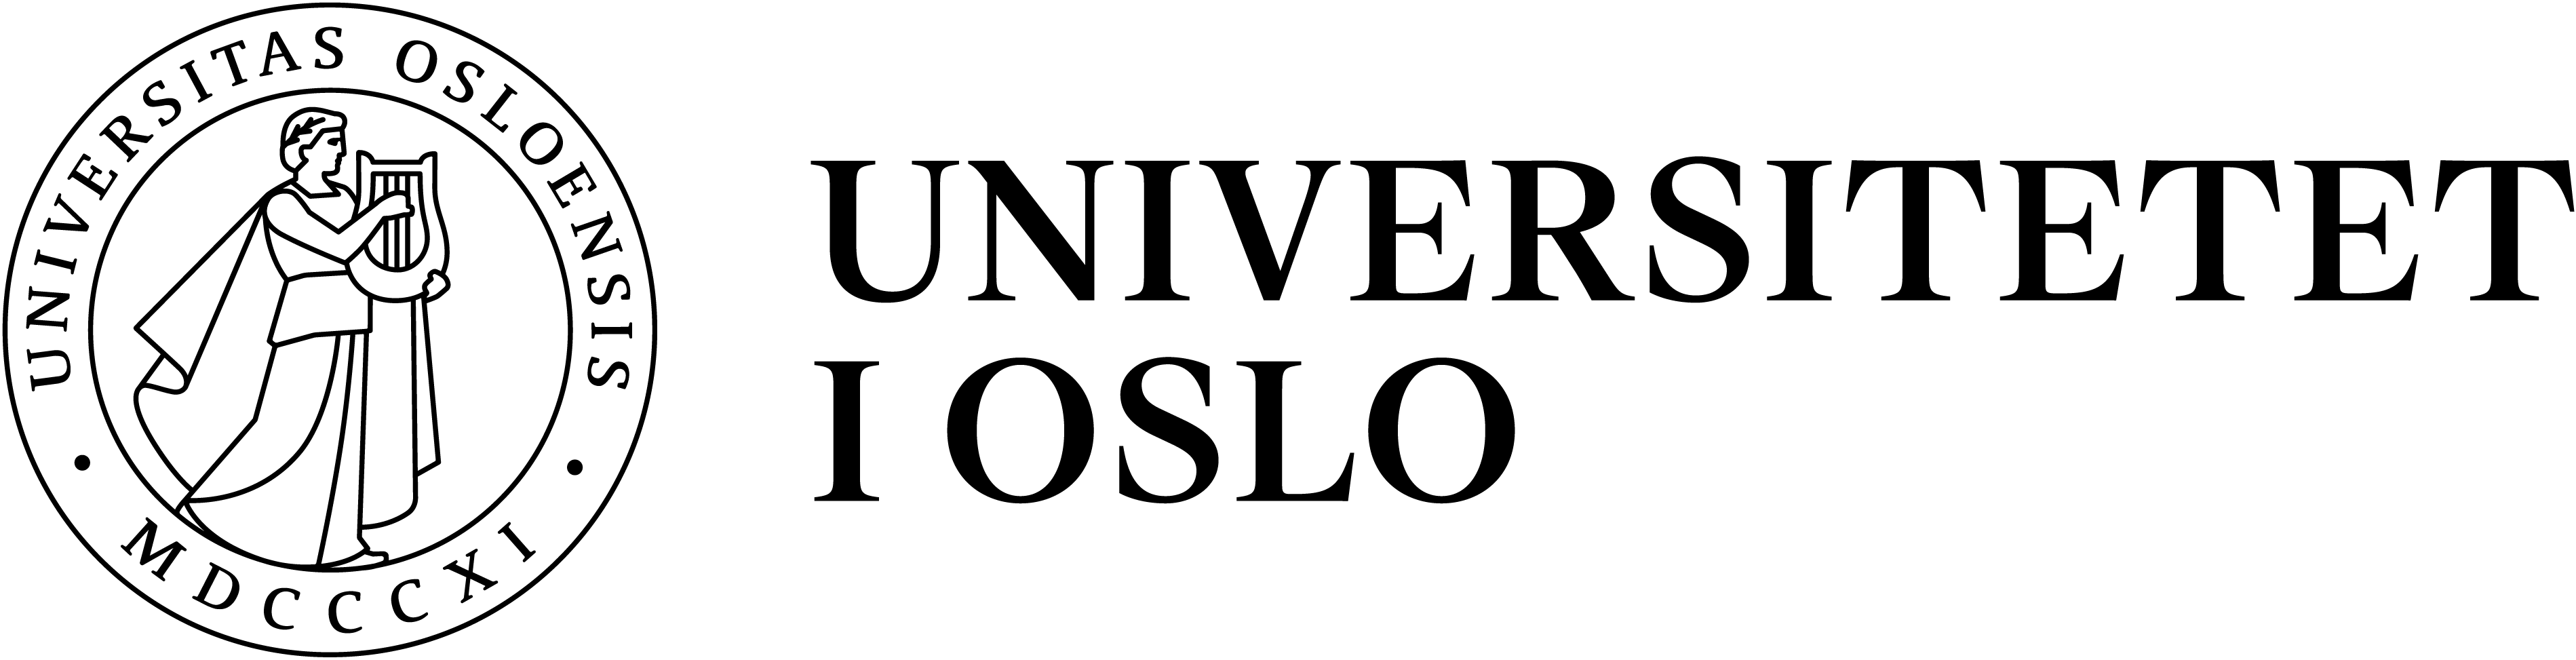
\includegraphics[width=\logowidth]{data/uio_logo_full.png}
}

\definecolor{ds002424}{HTML}{FF0028}
\definecolor{HBN}{HTML}{FF000E}
\definecolor{ABCD}{HTML}{FF0C00}
\definecolor{QTAB}{HTML}{FF2D00}
\definecolor{PING}{HTML}{FF4800}
\definecolor{ADHD200}{HTML}{FF6800}
\definecolor{PNC}{HTML}{FF8300}
\definecolor{ABIDE II}{HTML}{FFA400}
\definecolor{ds000119}{HTML}{FFBF00}
\definecolor{ABIDE I}{HTML}{FFDF00}
\definecolor{BRAINMINT}{HTML}{FFFA00}
\definecolor{SLIM}{HTML}{E8FF00}
\definecolor{QTIM}{HTML}{C7FF00}
\definecolor{Beijing}{HTML}{ACFF00}
\definecolor{AOMIC-PIOP2}{HTML}{8CFF00}
\definecolor{ds000202}{HTML}{71FF00}
\definecolor{AOMIC-PIOP1}{HTML}{51FF00}
\definecolor{AOMIC-ID1000}{HTML}{36FF00}
\definecolor{CoRR}{HTML}{15FF00}
\definecolor{HCP}{HTML}{00FF05}
\definecolor{FCON1000}{HTML}{00FF20}
\definecolor{ds000171}{HTML}{00FF40}
\definecolor{TOP}{HTML}{00FF5B}
\definecolor{SCZ-Z}{HTML}{00FF7B}
\definecolor{NIMH}{HTML}{00FF96}
\definecolor{NKI-RS}{HTML}{00FFB6}
\definecolor{MPI-LEMON}{HTML}{00FFD1}
\definecolor{ds003592}{HTML}{00FFF1}
\definecolor{ds004302}{HTML}{00F1FF}
\definecolor{ds000222}{HTML}{00D5FF}
\definecolor{SALD}{HTML}{00B5FF}
\definecolor{IXI}{HTML}{009AFF}
\definecolor{DLBS}{HTML}{0079FF}
\definecolor{Cam-CAN}{HTML}{005EFF}
\definecolor{StrokeMRI}{HTML}{003DFF}
\definecolor{PPMI}{HTML}{0022FF}
\definecolor{UKBB}{HTML}{0001FF}
\definecolor{Tao-Wu}{HTML}{1900FF}
\definecolor{ds000245}{HTML}{3400FF}
\definecolor{OASIS3}{HTML}{5500FF}
\definecolor{Demgen}{HTML}{7000FF}
\definecolor{NEUROCON}{HTML}{9000FF}
\definecolor{MIRIAD}{HTML}{AC00FF}
\definecolor{ds004392}{HTML}{CC00FF}
\definecolor{AIBL}{HTML}{E700FF}
\definecolor{ANM}{HTML}{FF00F5}
\definecolor{ADNI}{HTML}{FF00DA}

\begin{document}
	\begin{frame}
	 	\titlepage
	\end{frame}

    \begin{frame}{Oversikt}
        \begin{enumerate}
            \item Historien bak kunstig intelligens
            \item Hva er kunstig intelligens (og maskinlæring)
            \item Kunstig intelligens i hjerneforskning
        \end{enumerate}
    \end{frame}

	\section{Historien bak kunstig intelligens}

	\colorlet{activehistory}{uiored}
	\colorlet{passivehistory}{uiogray}
    \colorlet{nodefill}{yellow!75!red}

	\newcommand{\imagenetplot}[1]{
		\edef\stage{#1}
		\begin{tikzpicture}
			\begin{axis}[
				ylabel={Error rate},
				xlabel={År},
				xtick={2010, 2012, 2014, 2016, 2018, 2020},
				xticklabels={2010, 2012, 2014, 2016, 2018, 2020},
				ytick={0, 10, 20, 30},
				yticklabels={0\%, 10\%, 20\%, 30\%},
				ytick style={draw=none},
				ytick pos=left,
				xtick pos=bottom,
				ymajorgrids=true,
				ymax=29,
				ymin=0,
				xmin=2009,
				xmax=2021,
				width=8cm,
				height=5cm
			]
				\ifnum\stage=1
					\addplot[mark=*, cyan!60,thick] coordinates {
						(2010, 28.2)
						(2011, 25.8)
					};
				\fi
				\ifnum\stage=2
					\addplot[mark=*, cyan!60,thick] coordinates {
						(2010, 28.2)
						(2011, 25.8)
						(2012, 16.4)
					};
				\fi
				\ifnum\stage>2
					\addplot[mark=*, cyan!60,thick] coordinates {
						(2010, 28.2)
						(2011, 25.8)
						(2012, 16.4)
						(2013, 11.7)
						(2014, 7.3)
						(2015, 3.5)
						(2016, 3.0)
						(2017, 2.3)
						(2018, 1.8)
						(2019, 1.3)
						(2020, 0.9)
					};
				\fi

				\node[anchor=north, inner sep=5pt] at (axis cs: 2010, 28.2) {
					\small{28.2}
				};
				\node[anchor=north, inner sep=5pt] at (axis cs: 2011, 25.8) {
					\small{25.8}
				};

				\ifnum\stage>1
					\addplot[densely dotted] coordinates {
						(2011.5, 30)
						(2011.5, 0)
					};

					\node[anchor=north, inner sep=5pt] at (axis cs: 2012, 16.4) {
						\small{16.4}
					};
				\fi

				\ifnum\stage>2
					\node[anchor=north, inner sep=5pt] at (axis cs: 2013, 11.7) {
						\small{11.7}
					};
					\node[anchor=north, inner sep=5pt] at (axis cs: 2014, 7.3) {
						\small{7.3}
					};
					\node[anchor=north, inner sep=5pt] at (axis cs: 2015, 3.5) {
						\small{3.5}
					};
					\node[anchor=south, inner sep=5pt] at (axis cs: 2016, 3.0) {
						\small{3.0}
					};
					\node[anchor=south, inner sep=5pt] at (axis cs: 2017, 2.3) {
						\small{2.3}
					};
					\node[anchor=south, inner sep=5pt] at (axis cs: 2018, 1.8) {
						\small{1.8}
					};
					\node[anchor=south, inner sep=5pt] at (axis cs: 2019, 1.3) {
						\small{1.3}
					};
					\node[anchor=south, inner sep=5pt] at (axis cs: 2020, 0.9) {
						\small{\textbf{0.9}}
					};
				\fi

				\ifnum\stage>3
					\addplot[dashed, blue] coordinates {
						(2009, 5.1)
						(2021, 5.1)
					};

					\node[anchor=south east] at (axis cs: 2021, 5.1) {
						\textcolor{blue}{\small{Menneske}}
					};
				\fi

			\end{axis}
		\end{tikzpicture}
	}

	\newsavebox{\imagenetold}
	\sbox{\imagenetold}{%
		\imagenetplot{1}
	}

	\newsavebox{\imagenetcnn}
	\sbox{\imagenetcnn}{%
		\imagenetplot{2}
	}

	\newsavebox{\imagenetlatest}
	\sbox{\imagenetlatest}{%
		\imagenetplot{3}
	}

	\newsavebox{\imagenethuman}
	\sbox{\imagenethuman}{%
		\imagenetplot{4}
	}

    % \begin{frame}[t]{Historikk} % Turing
	% 	\newcommand{\historynode}[5]{
	% 		\node[
	% 			circle,
	% 			draw=####3,
	% 			fill=####3
	% 		] at (####1, -1) {};
	% 		\node[
	% 			anchor=####5,
	% 			####3,
	% 			align=center,
	% 			font=\small\linespread{0.95}\selectfont,
	% 			text height=9pt,
	% 			text depth=3pt,
	% 			inner sep=0pt,
	% 			align=center
	% 		] at (####1, ####2) {####4};
	% 	}

	% 	\begin{tikzpicture}
	% 		\node[] at (0, 0) {};
	% 		\node[] at (10.5, -7.5) {};

	% 		\draw[very thick, passivehistory] (0.5, -1)  -- (1.65, -1) {};
	% 		\onslide<3->{
	% 			\draw[very thick, passivehistory] (1.65, -1)  -- (2.35, -1) {};
	% 			\historynode{1.65}{-1.375}{passivehistory}{Turing\\(1950)}{north}
	% 		}
	% 		\onslide<5->{
	% 			\draw[very thick, passivehistory] (2.35, -1)  -- (2.68, -1) {};
	% 			\historynode{2.35}{-0.87}{passivehistory}{Dartmouth\\(1956)}{south}
	% 		}
	% 		\onslide<7->{
	% 			\draw[very thick, passivehistory] (2.68, -1)  -- (3.28, -1) {};
	% 			\historynode{2.68}{-1.375}{passivehistory}{Perceptron\\(1958)}{north}
	% 		}
	% 		\onslide<8->{
	% 			\draw[very thick, passivehistory] (3.28, -1)  -- (5.13, -1) {};
	% 			\historynode{3.28}{-0.87}{passivehistory}{Eliza\\(1964)}{south}
	% 		}
	% 		\onslide<9->{
	% 			\draw[very thick, passivehistory] (5.13, -1)  -- (5.82, -1) {};
	% 			\historynode{5.13}{-1.375}{passivehistory}{Ekspertsystemer\\(1980s)}{north}
	% 		}
	% 		\onslide<11->{
	% 			\draw[very thick, passivehistory] (5.82, -1)  -- (7.1, -1) {};
	% 			\historynode{5.82}{-0.87}{passivehistory}{Nevrale nettverk\\(1986)}{south}
	% 		}
	% 		\onslide<12->{
	% 			\draw[very thick, passivehistory] (7.1, -1)  -- (8.84, -1) {};
	% 			\historynode{7.10}{-1.372}{passivehistory}{Deep blue\\(1997)}{north}
	% 		}
	% 		\onslide<14->{
	% 			\draw[very thick, passivehistory] (8.84, -1)  -- (10, -1) {};
	% 			\historynode{8.84}{-0.87}{passivehistory}{Dyplæring\\(2012)}{south}
	% 		}

	% 		\only<1-2>{
	% 			\historynode{1.65}{-1.375}{activehistory}{Turing\\(1950)}{north}
	% 			\only<1>{
	% 				\node[inner sep=0pt, draw=black, label=below:{Alan Turing}] (patient) at (5.25, -4.25) {
	% 					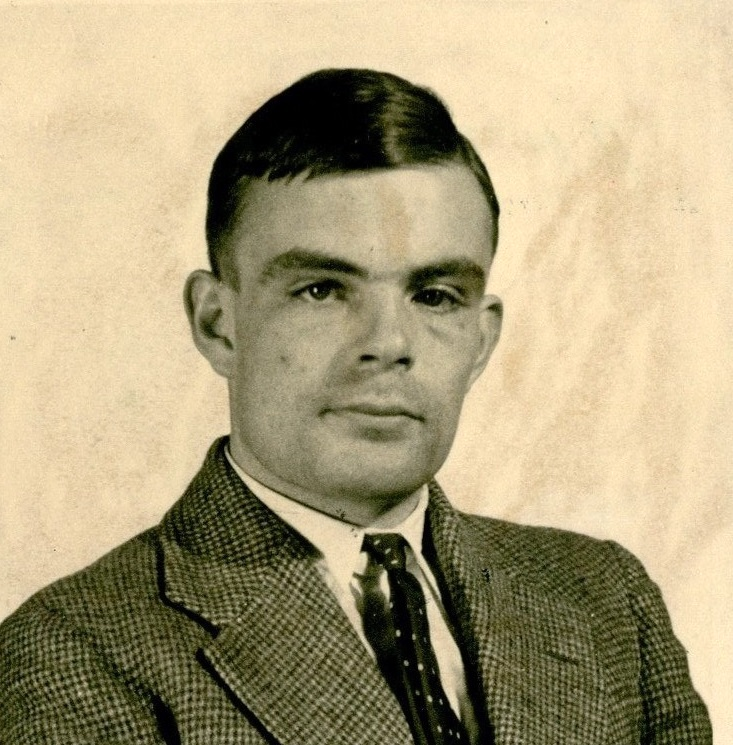
\includegraphics[width=4cm]{data/turing.jpeg}
	% 				};
	% 			}
	% 			\only<2>{
	% 				\node[inner sep=0pt, draw=black] (patient) at (5.25, -4.25) {
	% 					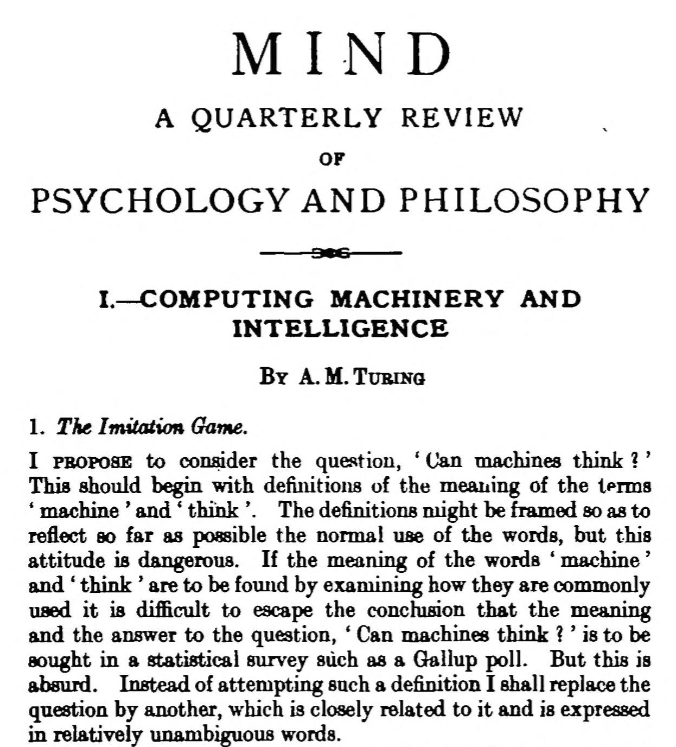
\includegraphics[width=4.5cm]{data/thinking.png}
	% 				};

	% 				\draw[uiored, thick] ($ (patient.east) - (0.2, 0.67) $) -- ($ (patient.east) - (1.75, 0.67) $);
	% 			}
	% 		}
	% 		\only<3-4>{
	% 			\historynode{2.35}{-0.87}{activehistory}{Dartmouth\\(1956)}{south}
	% 			\only<3>{
	% 				\node[inner sep=0pt] (patient) at (5.25, -4.75) {
	% 					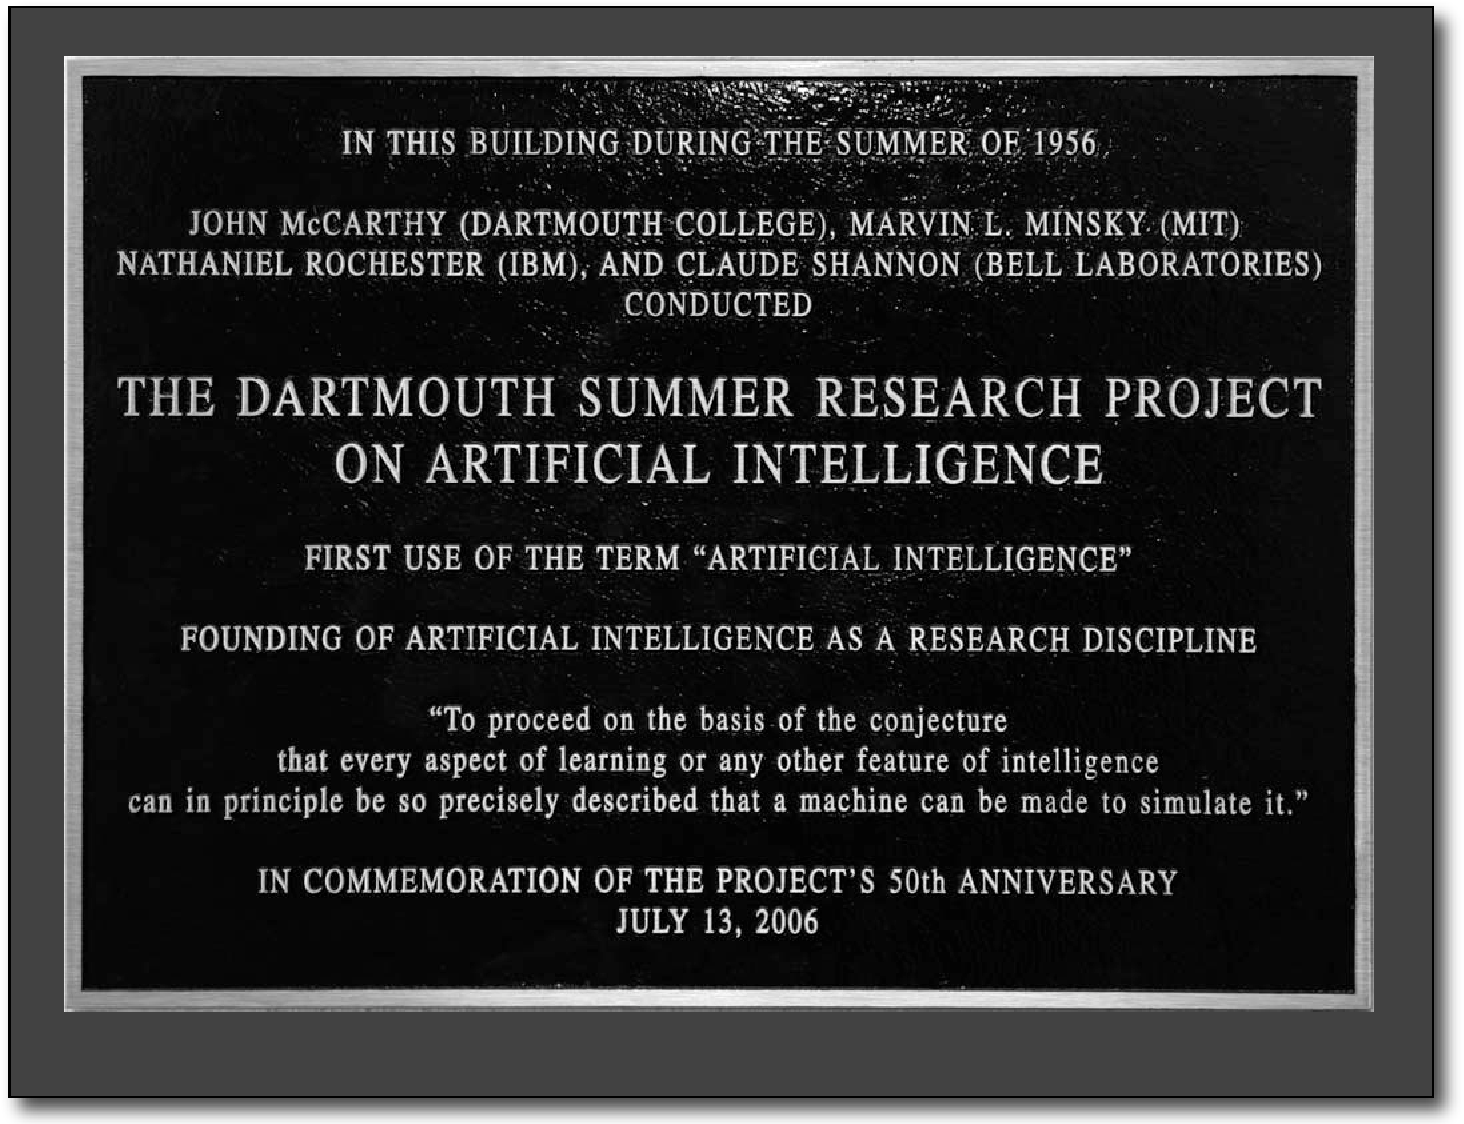
\includegraphics[width=6cm]{data/dartmouth.png}
	% 				};
	% 			}
	% 			\only<4>{
	% 				\node[inner sep=0pt, align=center] (patient) at (5.25, -4.75) {
	% 					"We propose that a 2-month, 10-man study of artificial intelligence\\
	% 					be carried out [...]. An attempt will be made to find how to make\\
	% 					machines use language, form abstractions and concepts, solve kinds\\
	% 					of problems now reserved for humans, and improve themselves. We think\\
	% 					that a significant advance can be made in [...] a summer."\\
	% 					\textbf{- Proposal, Dartmouth summer school (1956)}
	% 				};
	% 			}
	% 		}
	% 		\only<5-6>{
	% 			\historynode{2.68}{-1.375}{activehistory}{Perceptron\\(1958)}{north}
	% 			\node[draw=black, inner sep=5pt, fill=white] (patient) at (2.875, -4.75) {
	% 				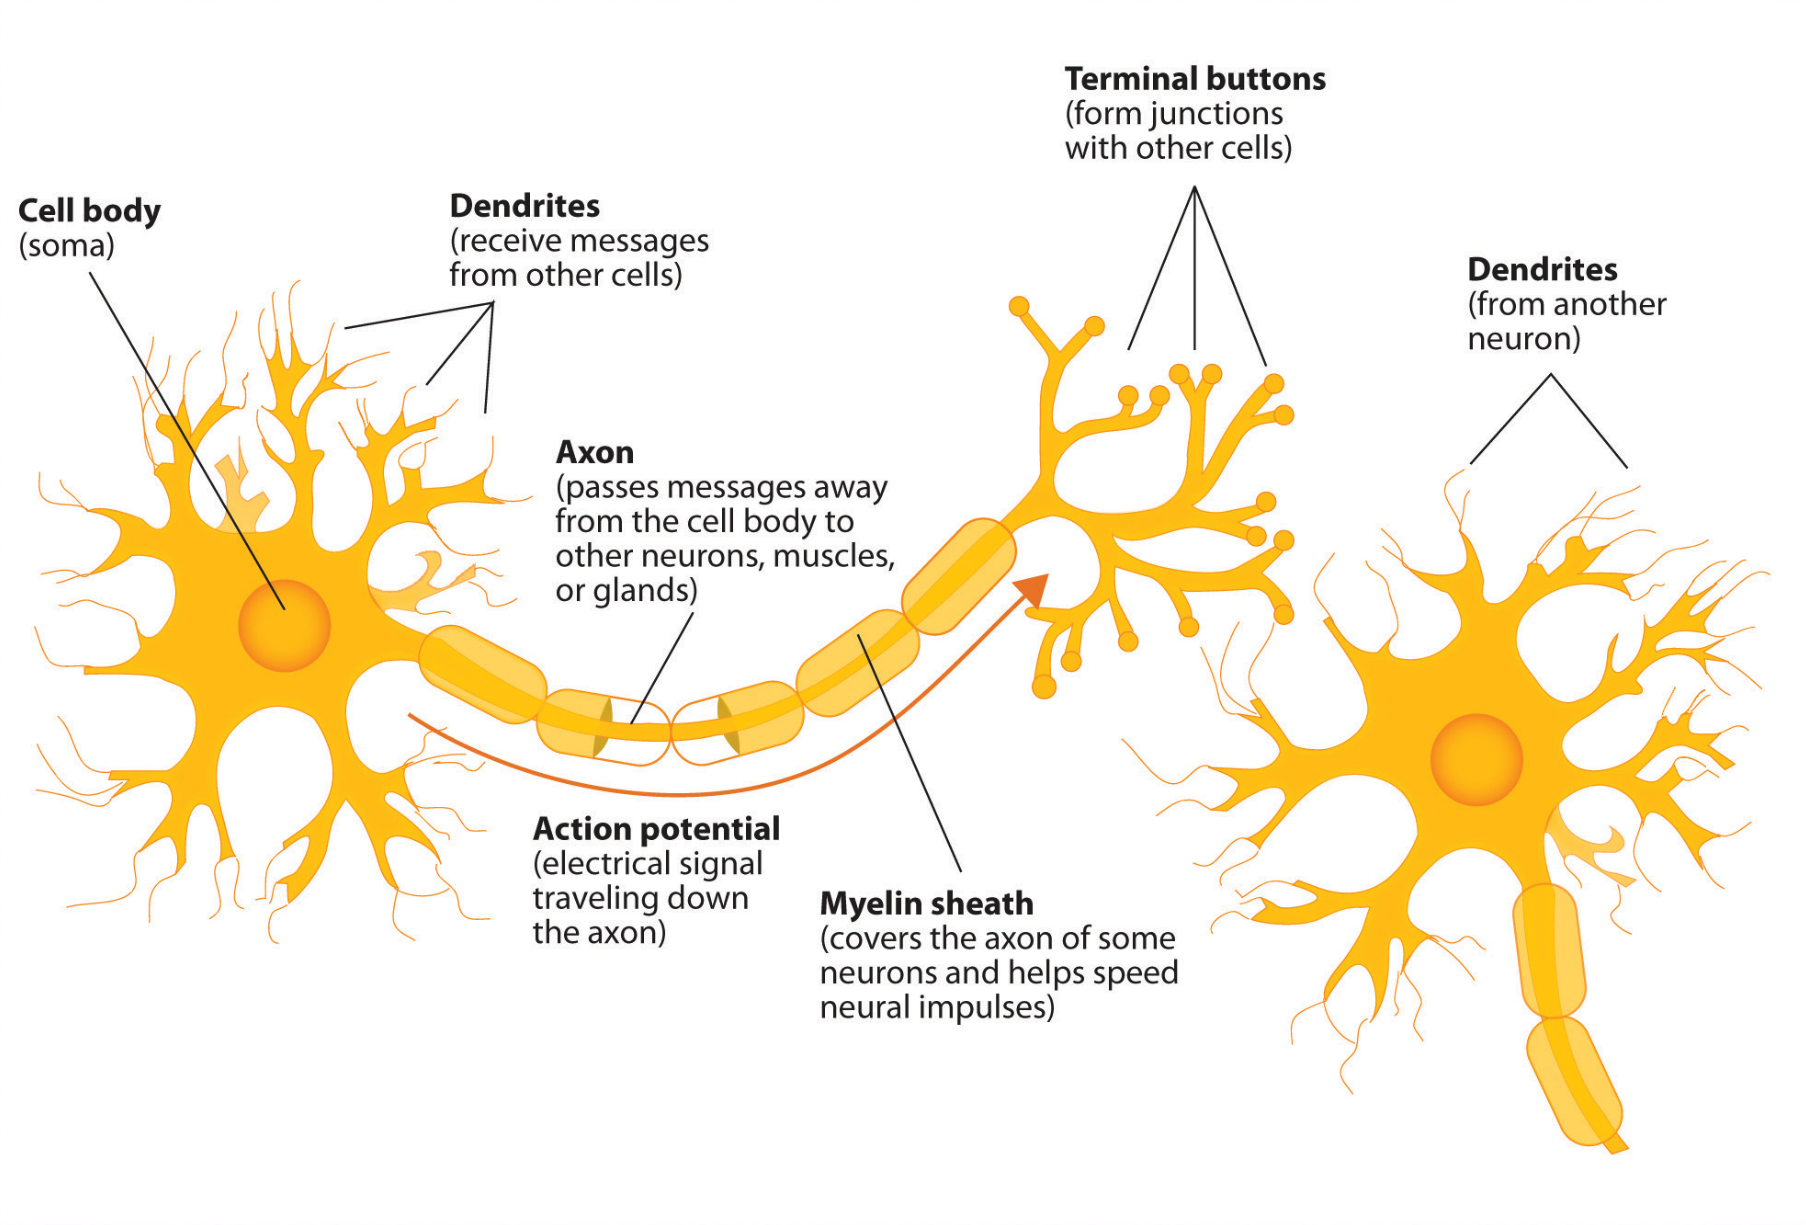
\includegraphics[width=4cm]{data/neuron.png}
	% 			};

	% 			\only<6>{
	% 				\node[draw=black, inner sep=5pt, fill=white] (patient) at (2.875, -4.75) {
	% 					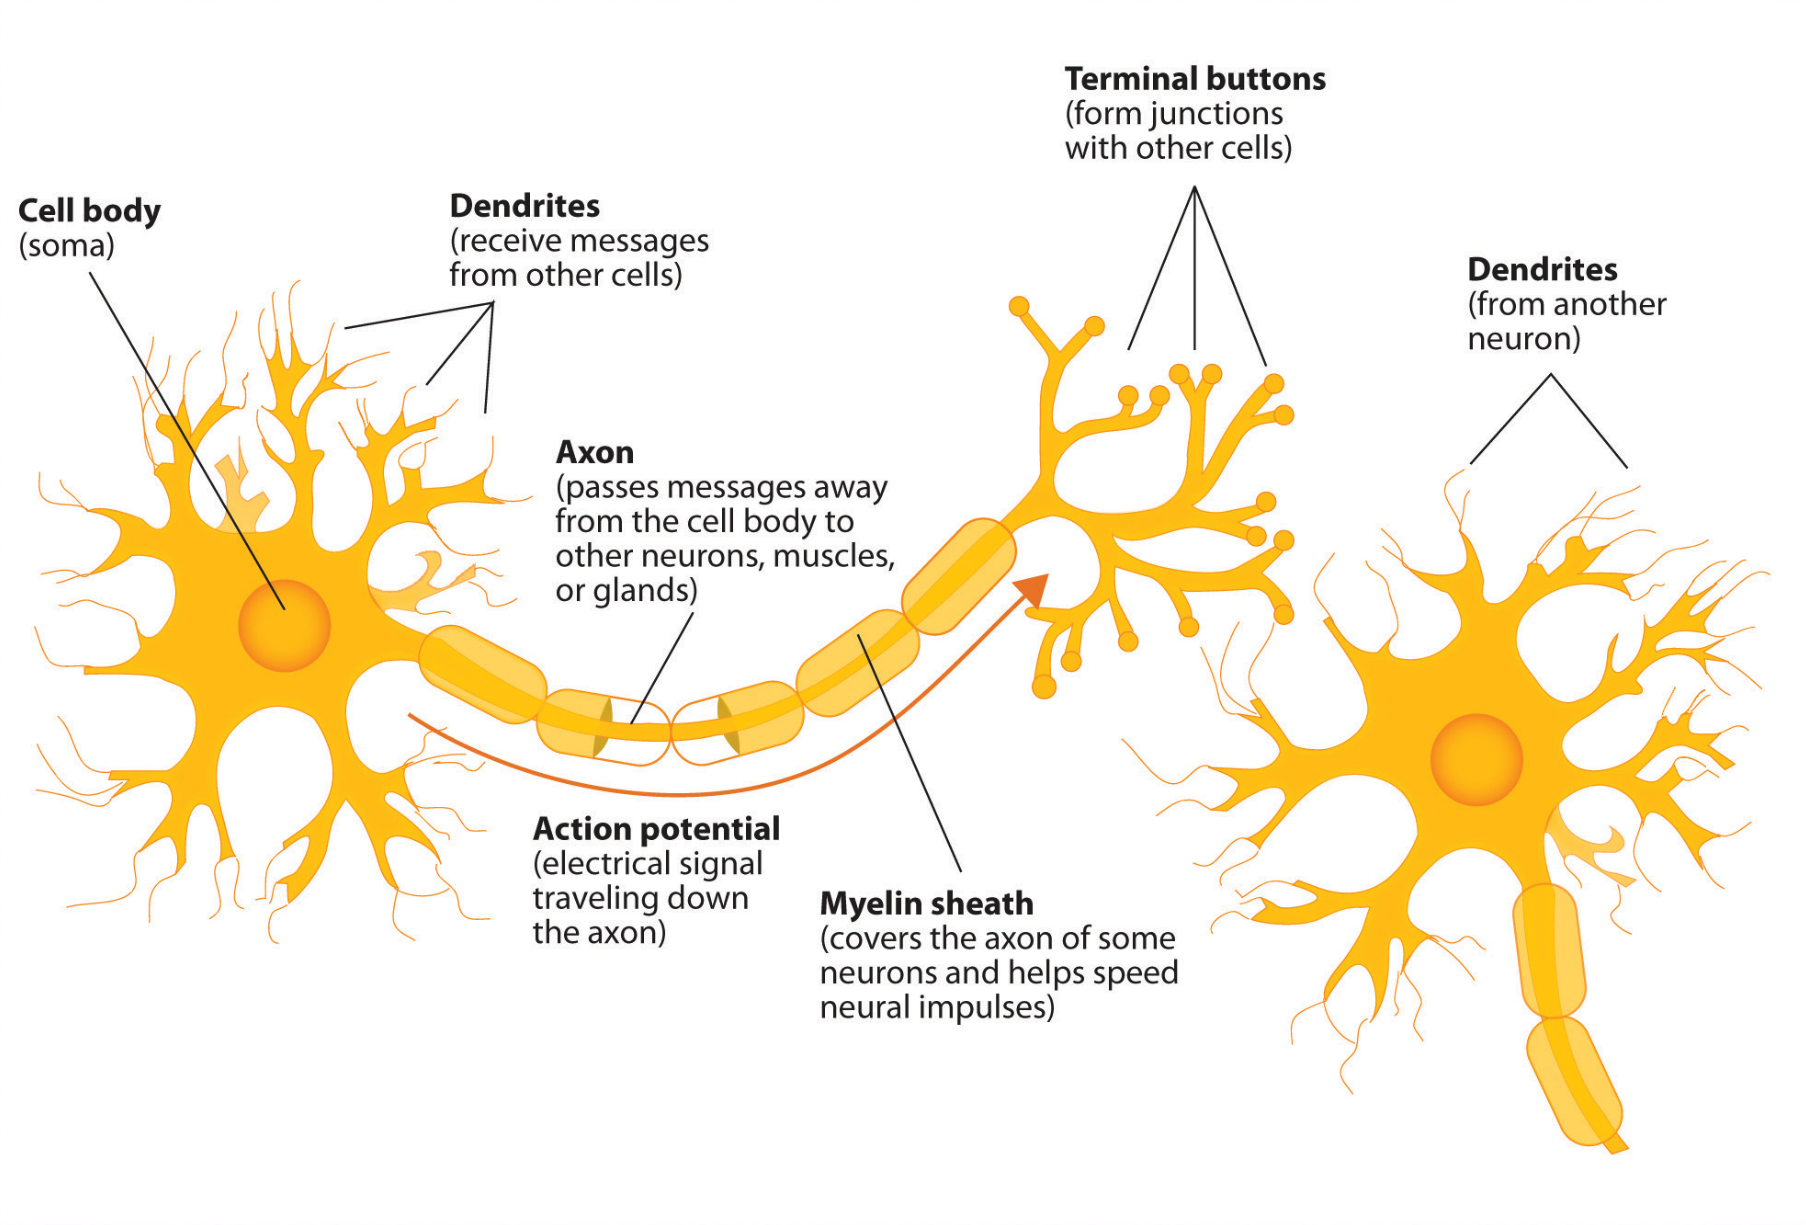
\includegraphics[width=4cm]{data/neuron.png}
	% 				};

	% 				\node[circle, draw=black, fill=nodefill, inner sep=2pt, text depth=0] (node) at (7.625, -4.75) {+};

	% 				\node[] (x0) at (6.375, -3.75) {$\mathrm{input}_0$};
	% 				\node[] (x1) at (6.375, -4.75) {$\mathrm{input}_1$};
	% 				\node[] (x2) at (6.375, -5.75) {$\mathrm{input}_2$};

	% 				\node[align=center] (out) at (8.875, -4.75) {$\mathrm{output}$\\$\mathrm{(0/1)}$};

	% 				\draw[-Latex] (x0) -- (node) node [midway, above] {\small{$w_0$}};
	% 				\draw[-Latex] (x1) -- (node) node [midway, below] {\small{$w_1$}};;
	% 				\draw[-Latex] (x2) -- (node) node [midway, below] {\small{$w_2$}};;
	% 				\draw[-Latex] (node) -- (out);
	% 			}
	% 		}
	% 		\only<7>{
	% 			\historynode{3.28}{-0.87}{activehistory}{Eliza\\(1964)}{south}
	% 			\node[draw=black, inner sep=5pt, fill=white, label=below:\small{https://web.njit.edu/\~ronkowit/eliza.html}] (patient) at (5.25, -4.75) {
	% 				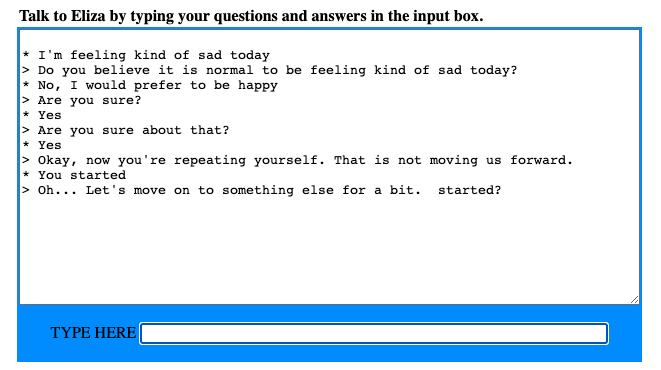
\includegraphics[width=7cm]{data/eliza.png}
	% 			};
	% 		}
	% 		\only<8>{
	% 			\historynode{5.13}{-1.375}{activehistory}{Ekspertsystemer\\(1980s)}{north}
	% 			\node[inner sep=0pt, draw=black, label=below:\small{MYCIN (1972)}] (patient) at (5.25, -4.75) {
	% 				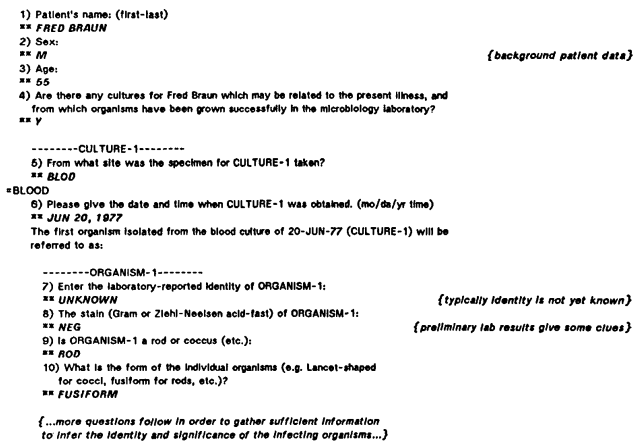
\includegraphics[width=6cm]{data/mycin.png}
	% 			};
	% 		}
	% 		\only<9-10>{
	% 			\historynode{5.82}{-0.87}{activehistory}{Nevrale nettverk\\(1986)}{south}


	% 			\only<9>{
	% 				\node[inner sep=0pt, minimum size=0.4cm, draw=black, circle, fill=nodefill] (n00) at (5.25, -4.75) {};

	% 				\node[] (x0) at (4, -4) {$\mathrm{input}_0$};
	% 				\node[] (x1) at (4, -4.75) {$\mathrm{input}_1$};
	% 				\node[] (x2) at (4, -5.5) {$\mathrm{input}_2$};

	% 				\node[] (out) at (6.5, -4.75) {$\mathrm{output}$};
	% 				\draw[-] (x0.east) -- (n00);
	% 				\draw[-] (x1.east) -- (n00);
	% 				\draw[-] (x2.east) -- (n00);

	% 				\draw[->] (n00) -- (out);
	% 			}
	% 			\only<10>{
	% 				\node[] (x0) at (2.5, -4) {$\mathrm{input}_0$};
	% 				\node[] (x1) at (2.5, -4.75) {$\mathrm{input}_1$};
	% 				\node[] (x2) at (2.5, -5.5) {$\mathrm{input}_2$};

	% 				\node[inner sep=0pt, minimum size=0.4cm, draw=black, circle, fill=nodefill] (n00) at (3.75, -3.75) {};
	% 				\node[inner sep=0pt, minimum size=0.4cm, draw=black, circle, fill=nodefill] (n01) at (3.75, -4.25) {};
	% 				\node[inner sep=0pt, minimum size=0.4cm, draw=black, circle, fill=nodefill] (n02) at (3.75, -4.75) {};
	% 				\node[inner sep=0pt, minimum size=0.4cm, draw=black, circle, fill=nodefill] (n03) at (3.75, -5.25) {};
	% 				\node[inner sep=0pt, minimum size=0.4cm, draw=black, circle, fill=nodefill] (n04) at (3.75, -5.75) {};

	% 				\node[inner sep=0pt, minimum size=0.4cm, draw=black, circle, fill=nodefill] (n10) at (4.5, -4) {};
	% 				\node[inner sep=0pt, minimum size=0.4cm, draw=black, circle, fill=nodefill] (n11) at (4.5, -4.5) {};
	% 				\node[inner sep=0pt, minimum size=0.4cm, draw=black, circle, fill=nodefill] (n12) at (4.5, -5) {};
	% 				\node[inner sep=0pt, minimum size=0.4cm, draw=black, circle, fill=nodefill] (n13) at (4.5, -5.5) {};

	% 				\node[inner sep=0pt, minimum size=0.4cm, draw=black, circle, fill=nodefill] (n20) at (5.25, -4.25) {};
	% 				\node[inner sep=0pt, minimum size=0.4cm, draw=black, circle, fill=nodefill] (n21) at (5.25, -4.75) {};
	% 				\node[inner sep=0pt, minimum size=0.4cm, draw=black, circle, fill=nodefill] (n22) at (5.25, -5.25) {};

	% 				\node[inner sep=0pt, minimum size=0.4cm, draw=black, circle, fill=nodefill] (n30) at (6, -4.5) {};
	% 				\node[inner sep=0pt, minimum size=0.4cm, draw=black, circle, fill=nodefill] (n31) at (6, -5) {};

	% 				\node[inner sep=0pt, minimum size=0.4cm, draw=black, circle, fill=nodefill, text depth=0] (n40) at (6.75, -4.75) {};
	% 				\node[] (out) at (8, -4.75) {$\mathrm{output}$};

	% 				\draw[-] (x0.east) -- (n00);
	% 				\draw[-] (x0.east) -- (n01);
	% 				\draw[-] (x0.east) -- (n02);
	% 				\draw[-] (x0.east) -- (n03);
	% 				\draw[-] (x0.east) -- (n04);
	% 				\draw[-] (x1.east) -- (n00);
	% 				\draw[-] (x1.east) -- (n01);
	% 				\draw[-] (x1.east) -- (n02);
	% 				\draw[-] (x1.east) -- (n03);
	% 				\draw[-] (x1.east) -- (n04);
	% 				\draw[-] (x2.east) -- (n00);
	% 				\draw[-] (x2.east) -- (n01);
	% 				\draw[-] (x2.east) -- (n02);
	% 				\draw[-] (x2.east) -- (n03);
	% 				\draw[-] (x2.east) -- (n04);

	% 				\draw[-] (n00) -- (n10);
	% 				\draw[-] (n00) -- (n11);
	% 				\draw[-] (n00) -- (n12);
	% 				\draw[-] (n00) -- (n13);
	% 				\draw[-] (n01) -- (n10);
	% 				\draw[-] (n01) -- (n11);
	% 				\draw[-] (n01) -- (n12);
	% 				\draw[-] (n01) -- (n13);
	% 				\draw[-] (n02) -- (n10);
	% 				\draw[-] (n02) -- (n11);
	% 				\draw[-] (n02) -- (n12);
	% 				\draw[-] (n02) -- (n13);
	% 				\draw[-] (n03) -- (n10);
	% 				\draw[-] (n03) -- (n11);
	% 				\draw[-] (n03) -- (n12);
	% 				\draw[-] (n03) -- (n13);
	% 				\draw[-] (n04) -- (n10);
	% 				\draw[-] (n04) -- (n11);
	% 				\draw[-] (n04) -- (n12);
	% 				\draw[-] (n04) -- (n13);

	% 				\draw[-] (n10) -- (n20);
	% 				\draw[-] (n10) -- (n21);
	% 				\draw[-] (n10) -- (n22);
	% 				\draw[-] (n11) -- (n20);
	% 				\draw[-] (n11) -- (n21);
	% 				\draw[-] (n11) -- (n22);
	% 				\draw[-] (n12) -- (n20);
	% 				\draw[-] (n12) -- (n21);
	% 				\draw[-] (n12) -- (n22);
	% 				\draw[-] (n13) -- (n20);
	% 				\draw[-] (n13) -- (n21);
	% 				\draw[-] (n13) -- (n22);

	% 				\draw[-] (n20) -- (n30);
	% 				\draw[-] (n20) -- (n31);
	% 				\draw[-] (n21) -- (n30);
	% 				\draw[-] (n21) -- (n31);
	% 				\draw[-] (n22) -- (n30);
	% 				\draw[-] (n22) -- (n31);

	% 				\draw[-] (n30) -- (n40);
	% 				\draw[-] (n31) -- (n40);

	% 				\draw[->] (n40) -- (out);
	% 			}
	% 		}
	% 		\only<11>{
	% 			\historynode{7.10}{-1.372}{activehistory}{Deep blue\\(1997)}{north}

	% 			\node[inner sep=0pt, draw=black, label=below:{\small{DALL-E: "A robot playing chess"}}] (img) at (2.75, -4.75) {
	% 				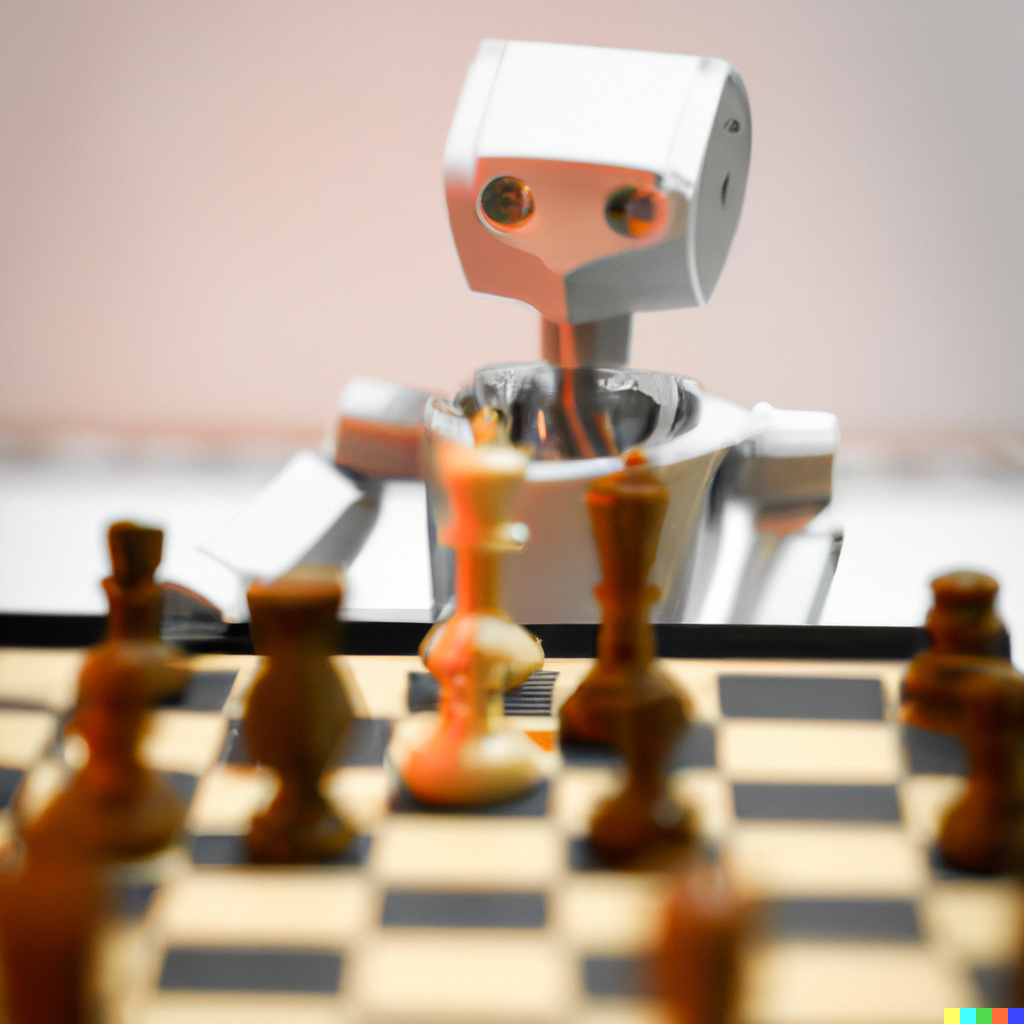
\includegraphics[width=4.3cm]{data/chess.png}
	% 			};
	% 			\node[anchor=north west, align=left] at ($ (img.north east)  + (0.1, 0) $) {
	% 				\bullet\hspace{0.1cm}IBMs Deep Blue ble den første\\datamaskinen som slo sittende\\verdensmester i sjakk.\\
	% 				\bullet\hspace{0.1cm}Deep blue vant med 3\textonehalf { }poeng mot\\Garry Kasparovs 2\textonehalf{ } etter seks spill.\\
	% 				\bullet\hspace{0.1cm}Kasparov har uttalt at "Deep Blue\\was intelligent the way your programmable\\alarm clock is intelligent."\\
	% 				\bullet\hspace{0.1cm}Avanserte søkealgoritmer og\\preprogrammert kunnskap fra\\sjakkeksperter.
	% 			};
	% 		}
	% 		\only<12-17>{
	% 			\historynode{8.84}{-0.87}{activehistory}{Dyplæring\\(2012)}{south}
	% 			\only<12-13>{
	% 				\node[inner sep=0pt, label=below:\small{Katt}] (img3) at (5.25, -4.75) {
	% 					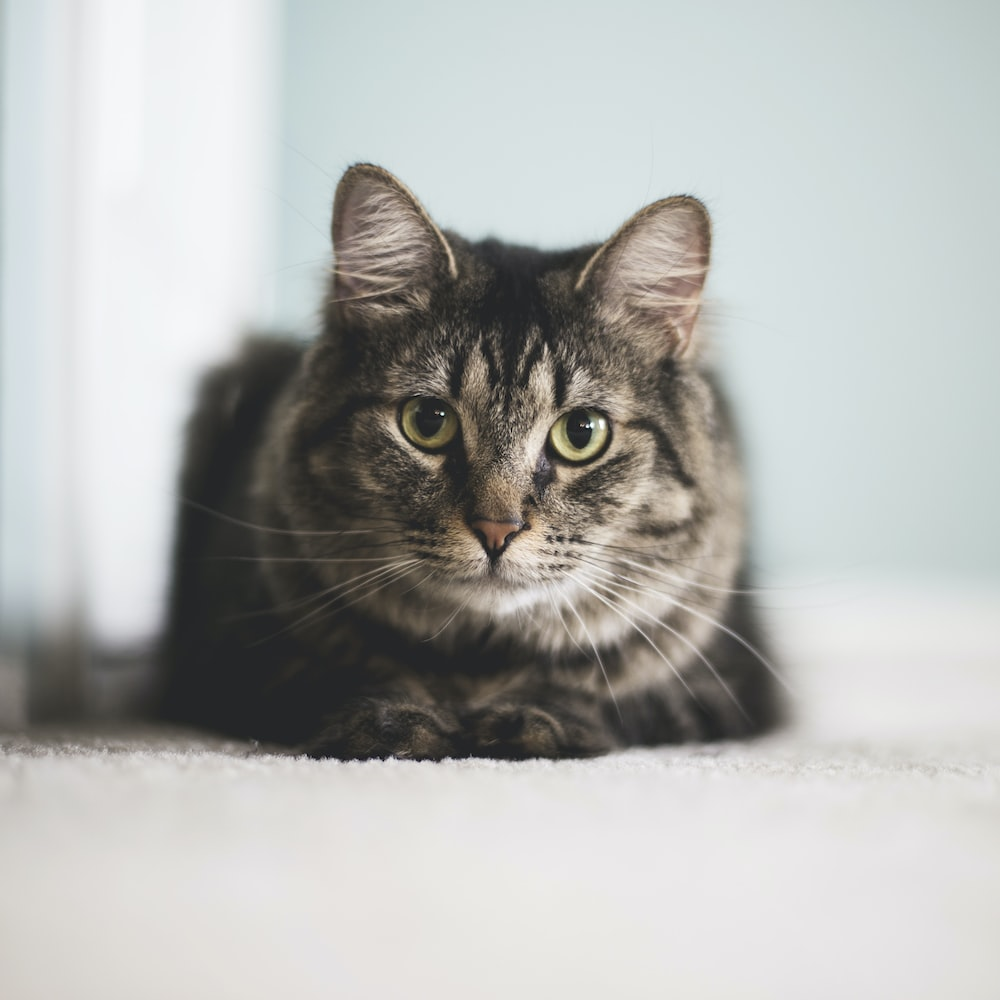
\includegraphics[width=1.5cm]{data/cat.jpeg}
	% 				};

	% 				\only<13>{
	% 					\node[inner sep=0pt, label=below:\small{Fly}, anchor=west] (img4) at ($ (img3.east) + (0.1, 0) $) {
	% 						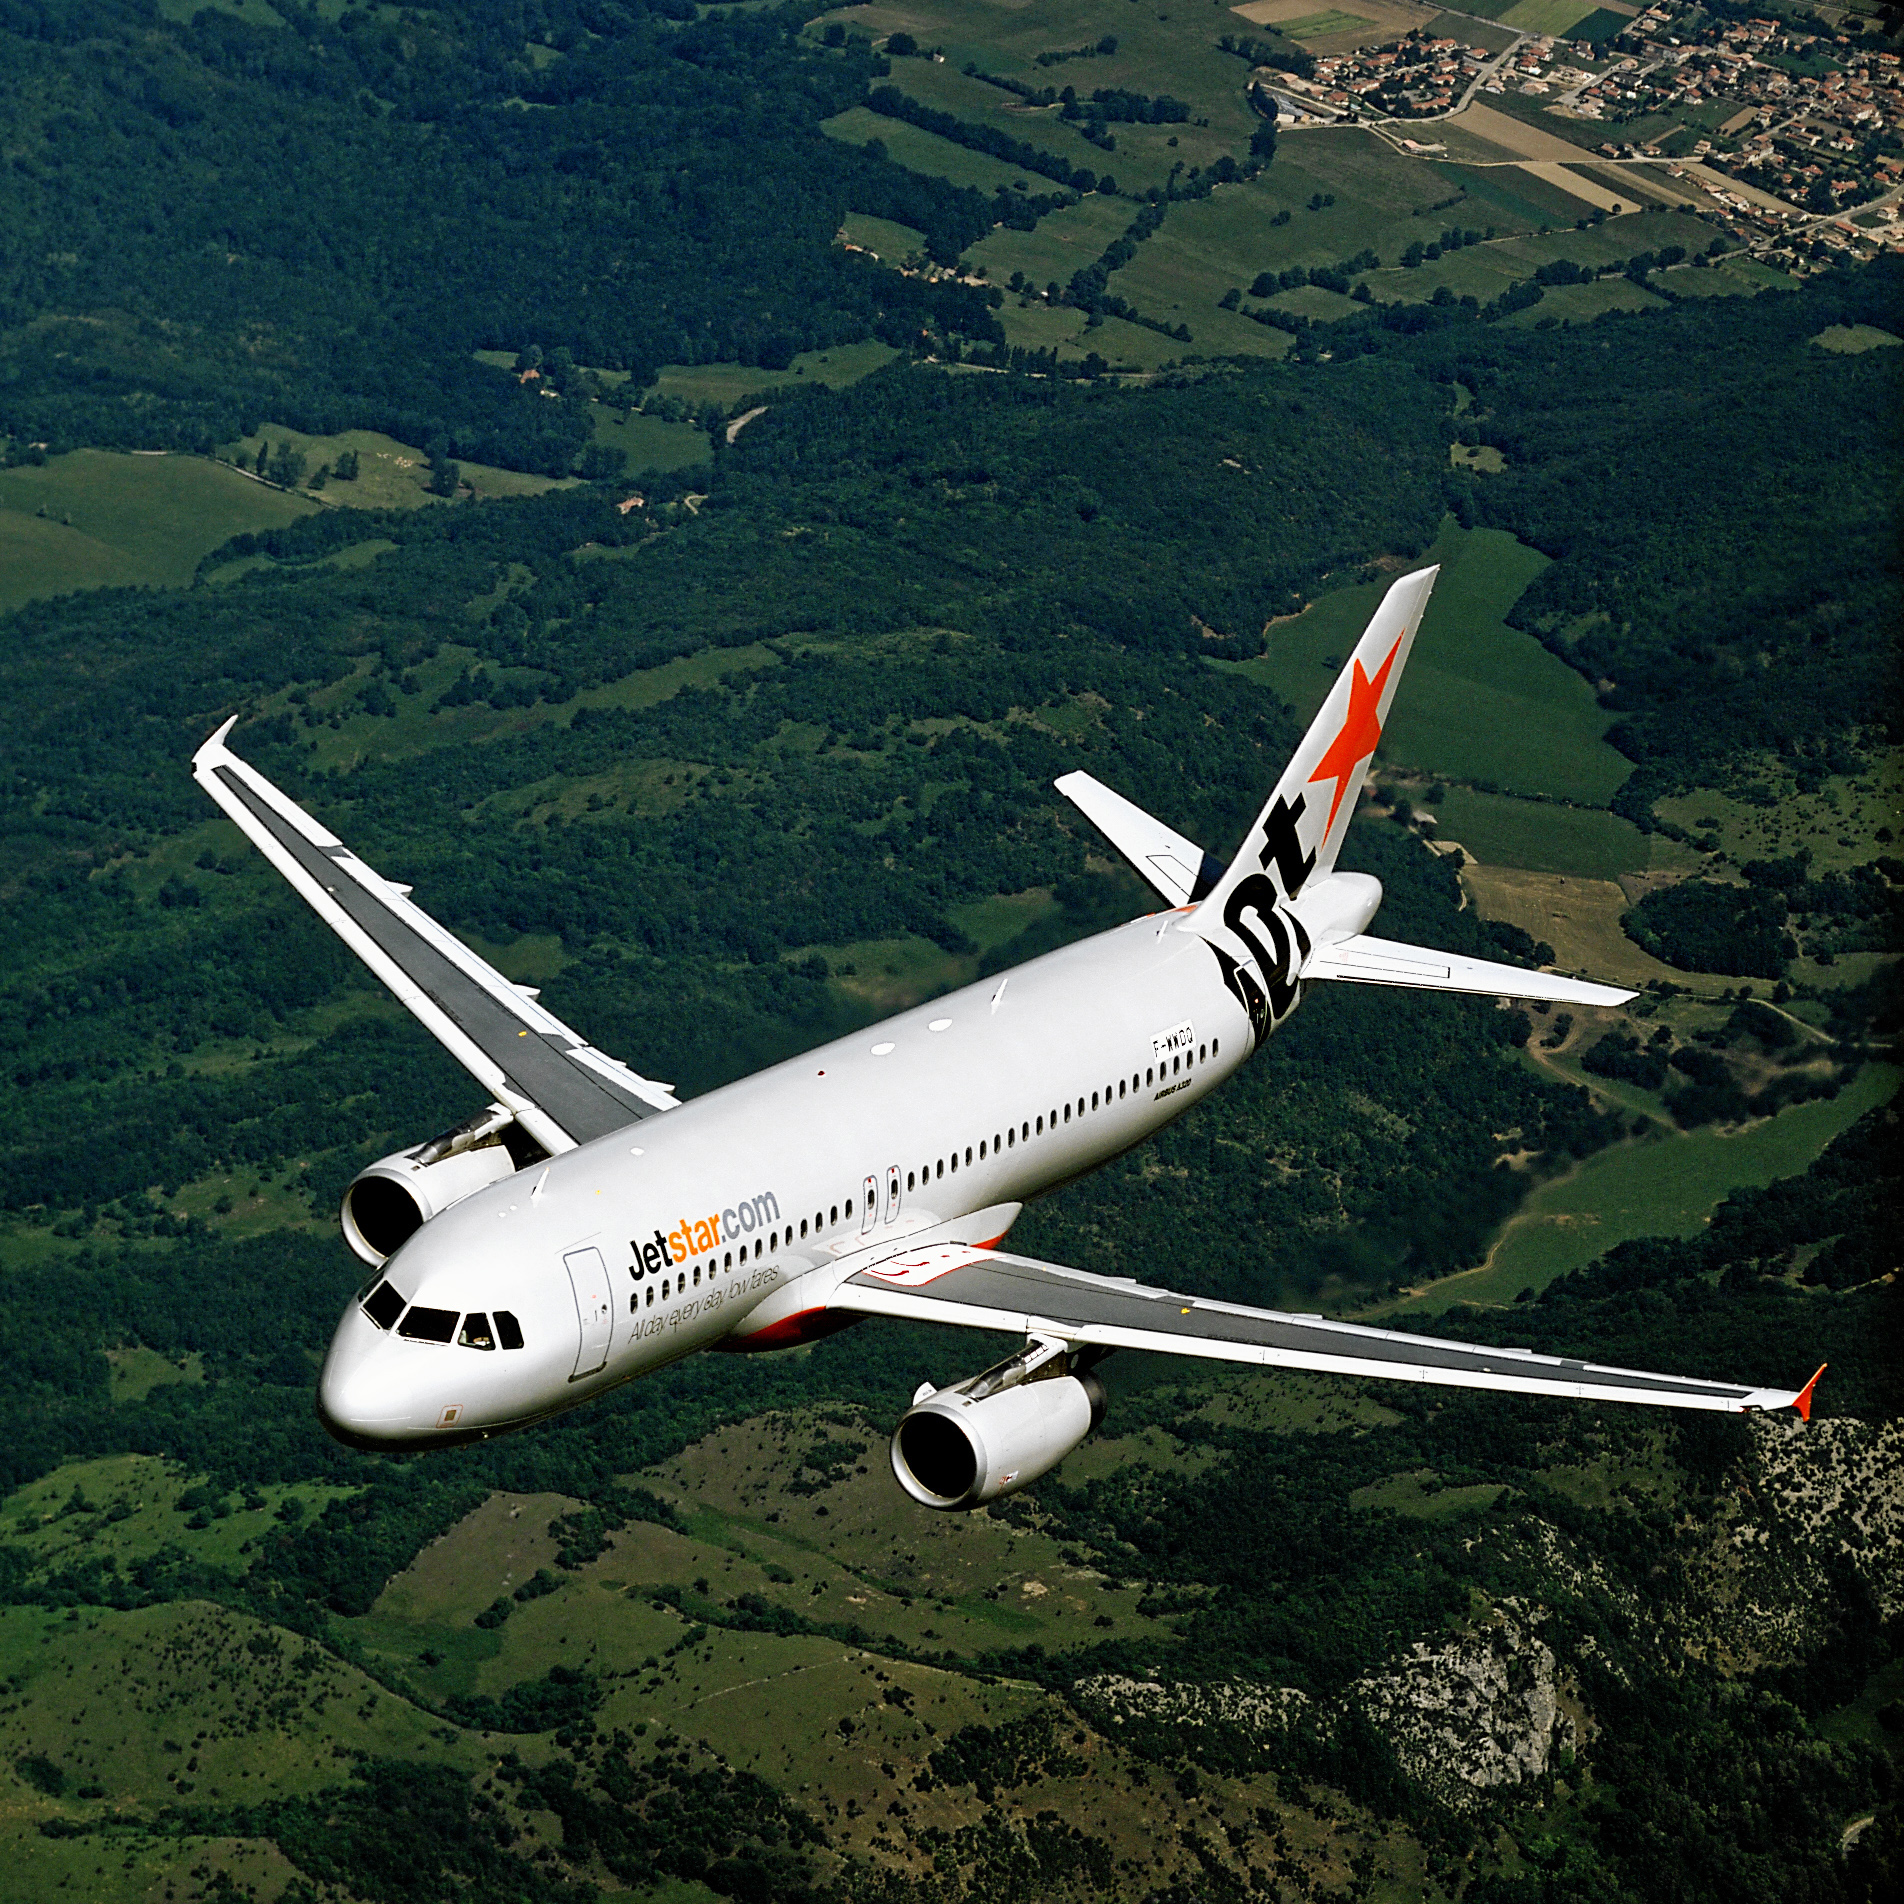
\includegraphics[width=1.5cm]{data/airplane.jpeg}
	% 					};
	% 					\node[inner sep=0pt, label=below:\small{Hvithai}, anchor=west] (img5) at ($ (img4.east) + (0.1, 0) $) {
	% 						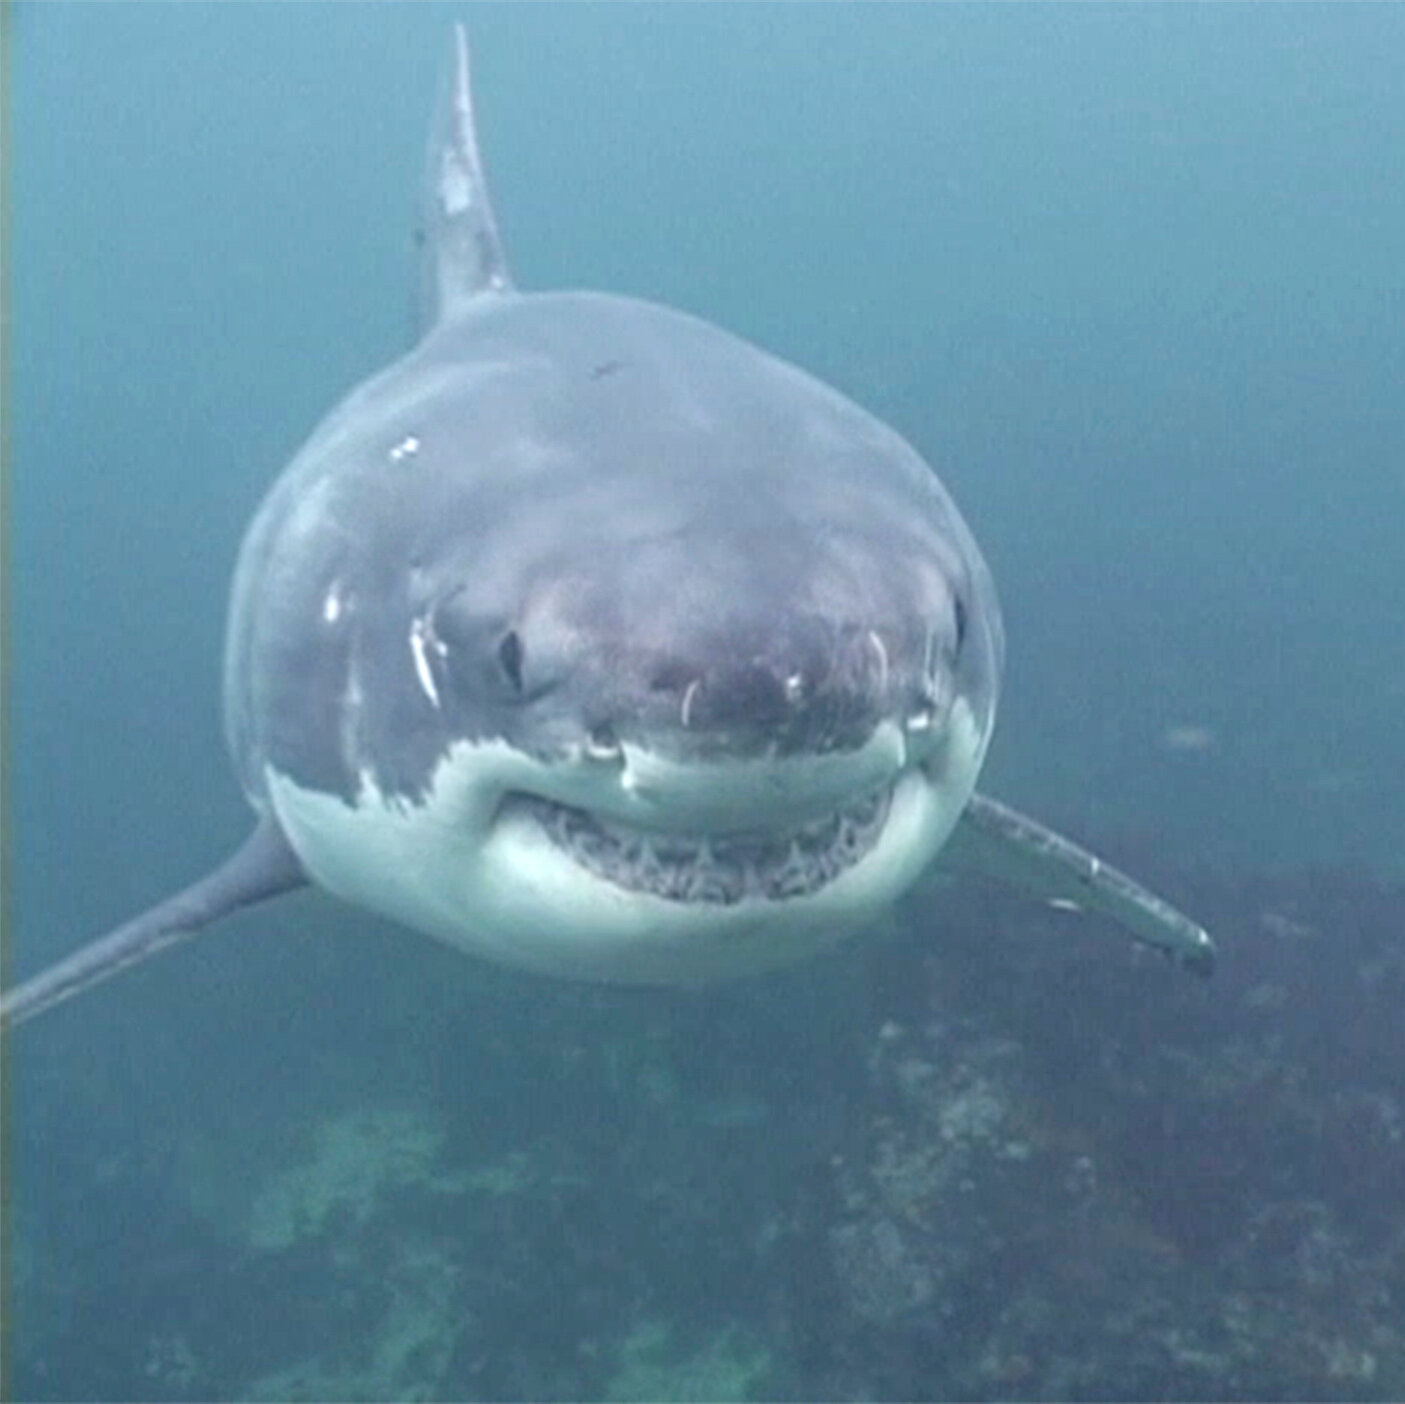
\includegraphics[width=1.5cm]{data/shark.jpeg}
	% 					};
	% 					\node[inner sep=0pt, label=below:\small{Marihøne}, anchor=east] (img2) at ($ (img3.west) - (0.1, 0) $) {
	% 						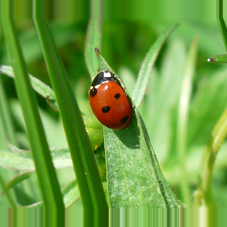
\includegraphics[width=1.5cm]{data/ladybug.png}
	% 					};
	% 					\node[inner sep=0pt, label=below:\small{Solsikke}, anchor=east] (img1) at ($ (img2.west) - (0.1, 0) $) {
	% 						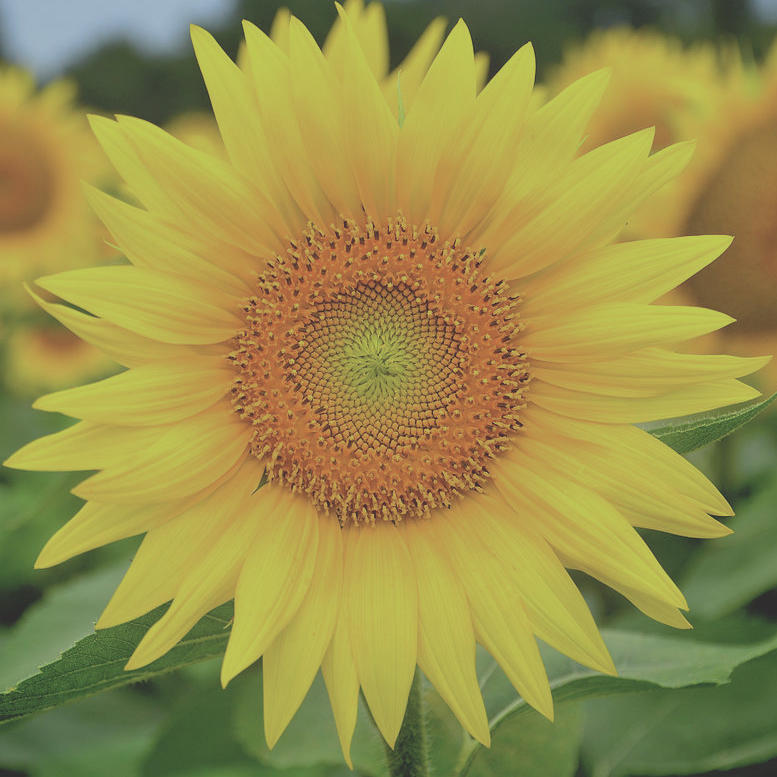
\includegraphics[width=1.5cm]{data/sunflower.jpeg}
	% 					};
	% 					\node[] at (5.25, -6.5) {
	% 						ImageNet: $\sim$14m bilder fra $\sim$22k kategorier
	% 					};
	% 				}
	% 			}
	% 			\only<14>{
	% 				\node[inner sep=0pt] at (5.25, -4.75) {
	% 					\usebox{\imagenetold}
	% 				};
	% 			}
	% 			\only<15>{
	% 				\node[inner sep=0pt] at (5.25, -4.75) {
	% 					\usebox{\imagenetcnn}
	% 				};
	% 			}
	% 			\only<16>{
	% 				\node[inner sep=0pt] at (5.25, -4.75) {
	% 					\usebox{\imagenetlatest}
	% 				};
	% 			}
	% 			\only<17>{
	% 				\node[inner sep=0pt] at (5.25, -4.75) {
	% 					\usebox{\imagenethuman}
	% 				};
	% 			}
	% 		}
	% 		\only<18>{
	% 			\historynode{10}{-1.33}{activehistory}{ChatGPT\\(2022)}{north}
	% 			\node[inner sep=0pt, draw=black] at (5.25, -4.75) {
	% 				
\includegraphics[width=5cm]{data/chatgpt.png}
	% 			};
	% 		}
	% 	\end{tikzpicture}
	% \end{frame}

    \section{Hva er egentlig kunstig intelligens (og maskinlæring)?}

    \begin{frame}{Hva er kunstig intelligens?} % Taxonomy, CNNs and LLMs
		\centering
		\vfill
		\begin{tikzpicture}
			\node[circle, fill=blue!60, minimum size=6cm] (ai) at (0, 0) {};
			\node[text=white, anchor=north] at ($ (ai.north) - (0, 0.3) $) {\textbf{Kunstig intelligens}};

			\only<2,12>{
				\node[text=white] at ($ (ai.north) - (-1.1, 1.2) $) {Symbolsk AI};
			}
			\onslide<13->{
				\node[circle, fill=purple!60, minimum size=4.5cm, anchor=south] (ml) at ($ (ai.south) + (0, 0.05) $) {};
				\node[text=white, anchor=north] at ($ (ml.north) - (0, 0.3) $) {\textbf{Maskinlæring}};
			}
			\onslide<14->{
				\node[text=white, align=center, font=\linespread{0.5}\selectfont] at ($ (ml.north) - (1, 1.1) $) {Lineær\\regresjon};
			}
			\onslide<15->{
				\node[circle, fill=red!60, minimum size=3cm, anchor=south] (dl) at ($ (ai.south) + (0, 0.1) $) {};
				\node[text=white, anchor=north] at ($ (dl.north) - (0, 0.3) $) {\textbf{Dyplæring}};
			}
			\onslide<16->{
				\node[align=center, text=white, font=\linespread{0.5}\selectfont] at ($ (dl.north) - (-0.2, 1.2) $) {Konvolusjonelle\\nevral nettverk};
				\node[align=center, text=white, font=\linespread{0.5}\selectfont] at ($ (dl.north) - (0.2, 2.1) $) {Store\\språkmodeller};
			}
			\only<1-2,12-16>{
				\only<1>{
					\node[anchor=north west, align=left, font=\small] (ai-text) at ($ (ai.north) + (3.5, 0.0) $) {\textbf{Kunstig intelligens (AI):}\\Maskiner som løser problemer\\som krever intelligens};
				}
				\onslide<2->{
					\node[anchor=north west, align=left, font=\small, text=gray!40] (ai-text) at ($ (ai.north) + (3.5, 0.0) $) {\textbf{Kunstig intelligens (AI):}\\Maskiner som løser problemer\\som krever intelligens};
				}
				\only<12>{
					\node[anchor=north west, align=left, font=\small] (ml-text) at ($ (ai-text.south west) - (0, 0) $) {\textbf{Symbolsk AI:}\\Tradisjonell AI der problemer\\løses gjennom oppslag mot regler,\\gjerne definert av menneskelige\\eksperter};
				}
				\only<13>{
					\node[anchor=north west, align=left, font=\small] (ml-text) at ($ (ai-text.south west) - (0, 0) $) {\textbf{Maskinlæring:}\\Maskiner som lærer å løse problemer\\gjennom å finne mønster i data på\\egenhånd};
				}
				\onslide<14->{
					\node[anchor=north west, align=left, font=\small, text=gray!40] (ml-text) at ($ (ai-text.south west) - (0, 0) $) {\textbf{Maskinlæring (ML):}\\Maskiner som lærer å løse problemer\\gjennom å finne mønster i data på\\egenhånd};
				}
				\only<14>{
					\node[anchor=north west, align=left, font=\small] (dl-text) at ($ (ml-text.south west) - (0, 0) $) {\textbf{Lineær regresion:}\\Maskinlæringsmodeller som \\finner lineære (m.a.o. enkle) mønstre};
				}
				\only<15>{
					\node[anchor=north west, align=left, font=\small] (dl-text) at ($ (ml-text.south west) - (0, 0) $) {\textbf{Dyplæring:}\\Maskinlæringsmodeller som er\\hierarkisk organisert ($\approx$ dype\\nevrale nettverk), inspirert av\\hjernens struktur};
				}
				\onslide<16->{
					\node[anchor=north west, align=left, font=\small, text=gray!40] (dl-text) at ($ (ml-text.south west) - (0, 0) $) {\textbf{Dyplæring:}\\Maskinlæringsmodeller som er\\hierarkisk organisert ($\approx$ dype\\nevrale nettverk), inspirert av\\hjernens struktur};
				}
				\only<16>{
					\node[anchor=north west, align=left, font=\small] (cnn-text) at ($ (dl-text.south west) - (0, 0) $) {\textbf{Konvolusjonelle nevrale nettverk:}\\Nevrale nettverk for prosessering\\av bildedata};
					\node[anchor=north west, align=left, font=\small] at ($ (cnn-text.south west) - (0, 0) $) {\textbf{Store språkmodeller:}\\(Store) nevrale nettverk\\for språkprosessering (f.eks. ChatGPT)};
				}
			}

			\only<3-11>{
				\def\outerwidth{2pt}
				\def\outercolour{gray!80}
				\def\offset{0.6}
				\colorlet{systemcolour}{gray!10}
				\colorlet{rulescolour}{blue!20}
				\colorlet{rulecolour}{cyan!20}

				\node[
					minimum width=3.8cm,
					minimum height=2.8cm,
					draw=black,
					fill=systemcolour,
					label=above:{\textbf{\small{PSYCIN}}}
				] (system) at (5.5, -1) {};

				\onslide<4->{
					\node[] (doctor) at (5.5, 2.5) {
						\Huge{\emoji{woman-health-worker}}
					};
				}
				\onslide<5->{
					\node[] (notes) at (5.5 - \offset, 1.25) {
						\Huge{\emoji{spiral-notepad}}
					};
					\draw[-stealth, line width=\outerwidth, \outercolour]
						(doctor) to [out=270, in=90]
						(notes) --
						($ (system.north) - (\offset, 0) $);
				}

				\onslide<6->{
					\node[
						minimum width=2.4cm,
						minimum height=1.6cm,
						draw=black,
						fill=rulescolour,
						label=above:{\textbf{\footnotesize{Regelmotor}}}
					] (rules) at ($ (system) - (0, 0.5) $) {};
					\draw[-stealth, line width=\outerwidth, \outercolour]
						($ (system.north) - (\offset, 0) $) to [in=0, out=270]
						($ (rules.north west) + (-0.2, 0.2) $) to [in=180, out=180]
						($ (rules.west) - (0.2, 0) $) --
						(rules.west);
				}
				\onslide<7->{
					\node[
						minimum width=1.5cm,
						minimum height=0.3cm,
						draw=black,
						fill=rulecolour
					] (rule1) at ($ (rules) + (0, 0.5) $) {
						\small{Nedstemt}
					};
					\node[
						minimum width=1.5cm,
						minimum height=0.3cm,
						draw=black,
						fill=rulecolour
					] (rule2) at ($ (rules) + (0, 0.0) $) {
						\small{Søvnløshet}
					};
					\node[
						minimum width=1.5cm,
						minimum height=0.3cm,
						draw=black,
						fill=rulecolour
					] (rule3) at ($ (rules) + (0, -0.5) $) {
						\small{Tretthet}
					};
					\draw[] (rules.west) to [in=180, out=0] (rule1.west);
					\draw[] (rules.west) to [in=180, out=0] (rule2.west);
					\draw[] (rules.west) to [in=180, out=0] (rule3.west);

					\draw[] (rule1.east) to [in=180, out=0] (rules.east);
					\draw[] (rule2.east) to [in=180, out=0] (rules.east);
					\draw[] (rule3.east) to [in=180, out=0] (rules.east);
				}

				\onslide<8->{
					\draw[-stealth, line width=\outerwidth, \outercolour]
						(rules.east) --
						($ (rules.east) + (0.2, 0) $) to [out=0, in=0]
						($ (rules.north east) + (0.2, 0.2) $) to [out=180, in=270]
						($ (system.north) + (\offset, 0) $);

					\node[minimum height=0.75cm] (diagnosis) at (5.5 + \offset, 1.25) {
						\small{Depresjon}
					};

					\draw[line width=\outerwidth, \outercolour]
						($ (system.north) + (\offset, 0) $) --
						(diagnosis) to [out=90, in=270]
						(doctor);
				}
				\only<9>{
					\draw[red, thick] (system.north east) -- (system.north west) -- (system.south west) -- (system.south east) -- cycle;
					\draw[red, thick] (rules.north east) -- (rules.north west) -- (rules.south west) -- (rules.south east) -- cycle;
				}
				\onslide<10->{
					\draw[red!20, thick] (system.north east) -- (system.north west) -- (system.south west) -- (system.south east) -- cycle;
					\draw[red!20, thick] (rules.north east) -- (rules.north west) -- (rules.south west) -- (rules.south east) -- cycle;
				}
				\only<10>{
					\draw[red, thick] (notes.north east) -- (notes.north west) -- (notes.south west) -- (notes.south east) -- cycle;
				}
				\onslide<11->{
					\draw[red!20, thick] (notes.north east) -- (notes.north west) -- (notes.south west) -- (notes.south east) -- cycle;
				}
				\only<11>{
					\node[] (scientist) at ($ (system.south) - (0, 1) $) {
						\Huge{\emoji{man-scientist}}
					};

					\draw[red, thick] (rule1.north east) -- (rule1.north west) -- (rule1.south west) -- (rule1.south east) -- cycle;
					\draw[red, thick] (rule2.north east) -- (rule2.north west) -- (rule2.south west) -- (rule2.south east) -- cycle;
					\draw[red, thick] (rule3.north east) -- (rule3.north west) -- (rule3.south west) -- (rule3.south east) -- cycle;
					\draw[-stealth, red, thick, dashed] (scientist) -- (rule3);
				}
			}



			%\node[anchor=north west, align=left, font=\small, text=gray!40] (dl-text) at ($ (ml-text.south west) - (0, 0) $) {\textbf{Dyplæring:}\\Maskinlæringsmodeller som er\\hierarkisk organisert ($\approx$ dype\\nevrale nettverk), inspirert av\\hjernens struktur};
			%\node[anchor=north west, align=left, font=\small] (cnn-text) at ($ (dl-text.south west) - (0, 0) $) {\textbf{Konvolusjonelle nevrale nettverk:}\\Nevrale nettverk for prosessering\\av bildedata};
			%\node[anchor=north west, align=left, font=\small] at ($ (cnn-text.south west) - (0, 0) $) {\textbf{Store språkmodeller:}\\(Store) nevrale nettverk\\for språkprosessering (ChatGPT)};
			\node[] at (-3, 3) {};
			\node[] at (7.7, -4) {};
		\end{tikzpicture}
		\vfill
	\end{frame}

    \begin{frame}{Hva er kunstig intelligens?} % Taxonomy, CNNs and LLMs
		\centering
		\vfill
		\begin{tikzpicture}
			\node[circle, fill=blue!60, minimum size=6cm] (ai) at (0, 0) {};
			\node[text=white, anchor=north] at ($ (ai.north) - (0, 0.3) $) {\textbf{Kunstig intelligens}};
			\node[anchor=north west, align=left, font=\small] (ai-text) at ($ (ai.north) + (3.5, 0.0) $) {\textbf{Kunstig intelligens (AI):}\\Maskiner som løser problemer\\som krever intelligens};
			\node[] at (-3, 3) {};
			\node[] at (7.7, -3.2) {};
		\end{tikzpicture}
		\vfill
	\end{frame}

    \begin{frame}{Hva er kunstig intelligens?} % Taxonomy, CNNs and LLMs
		\centering
		\vfill
		\begin{tikzpicture}
			\node[circle, fill=blue!60, minimum size=6cm] (ai) at (0, 0) {};
			\node[text=white, anchor=north] at ($ (ai.north) - (0, 0.3) $) {\textbf{Kunstig intelligens}};
			\node[text=white] at ($ (ai.north) - (-1.1, 1.2) $) {Symbolsk AI};
			\node[anchor=north west, align=left, font=\small] (ai-text) at ($ (ai.north) + (3.5, 0.0) $) {\textbf{Kunstig intelligens (AI):}\\Maskiner som løser problemer\\som krever intelligens};
			\node[] at (-3, 3) {};
			\node[] at (7.7, -3.2) {};
		\end{tikzpicture}
		\vfill
	\end{frame}

    \begin{frame}{Hva er kunstig intelligens?} % Symbolic: Setup
        \centering
        \begin{tikzpicture}
            \node[draw=black, minimum height=4.6cm, minimum width=7cm, fill=blue!10] (mycin) at (0, 0) {};

            \node[inner sep=0pt, draw=black] (interface) at (mycin.north) {
                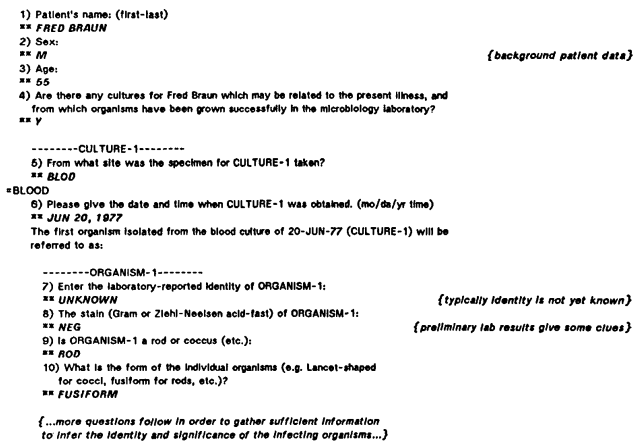
\includegraphics[width=4cm, trim={0 11cm 5.5cm 0},clip]{data/mycin.png}
            };
            \node[anchor=south east] at (mycin.north east) {MYCIN};

            \node[] (patient) at ($ (interface.north) + (0, 1.2) $) {
               \Huge{\emoji{face-with-thermometer}}
            };

            \draw[gray, very thick, Latex-Latex] (patient) -- (interface);
             \node[] at (-4, 4.3) {};
             \node[] at (4, -3.45) {};

        \end{tikzpicture}
	\end{frame}

    \begin{frame}{Hva er kunstig intelligens?} % Symbolic: Brain
        \centering
        \begin{tikzpicture}
            \node[draw=black, minimum height=4.6cm, minimum width=7cm, fill=blue!10] (mycin) at (0, 0) {};
            \node[draw=black, minimum height=2.2cm, minimum width=4cm, dashed] (db) at ($ (mycin) - (0, 0.7) $) {};
            \node[anchor=south, font=\small] at (db.north) {Prediktiv modell};

            \node[inner sep=0pt, draw=black] (interface) at (mycin.north) {
                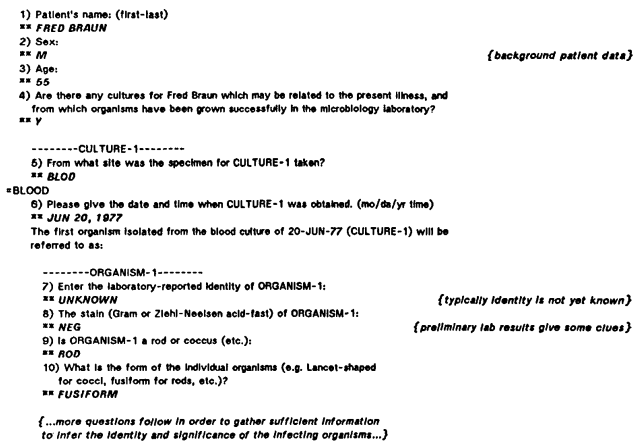
\includegraphics[width=4cm, trim={0 11cm 5.5cm 0},clip]{data/mycin.png}
            };
            \node[anchor=south east] at (mycin.north east) {MYCIN};

            \draw[gray, very thick, -Latex] ($ (interface.south) - (0.2, 0) $) to [out=270,in=0] ($ (db.west) + (0, 1.8) $) to [out=180,in=180] (db.west) {};
            \draw[gray, very thick, Latex-] ($ (interface.south) + (0.2, 0) $) to [out=270,in=180] ($ (db.east) + (0, 1.8) $) to [out=0,in=0] (db.east) {};

            \node[] (patient) at ($ (interface.north) + (0, 1.2) $) {
               \Huge{\emoji{face-with-thermometer}}
            };

            \draw[gray, very thick, Latex-Latex] (patient) -- (interface);

             \node[anchor=south, text depth=0] at ($ (db.west) + (0.6, 1.8) $) {\small{Data}};
             \node[anchor=south, text depth=0] at ($ (db.east) + (-0.6, 1.8) $) {\small{Prediksjon}};
             \node[] at (-4, 4.3) {};
             \node[] at (4, -3.45) {};

        \end{tikzpicture}
	\end{frame}

    \begin{frame}{Hva er kunstig intelligens?} % Symbolic: Rules
        \centering
        \begin{tikzpicture}
            \node[draw=black, minimum height=4.6cm, minimum width=7cm, fill=blue!10] (mycin) at (0, 0) {};
            \node[draw=black, minimum height=2.2cm, minimum width=4cm, dashed] (db) at ($ (mycin) - (0, 0.7) $) {};
            \node[anchor=south, font=\small] at (db.north) {Kunnskapsdatabase};

            \node[draw=black, minimum width=2.4cm, anchor=south, fill=cyan!10] (fever) at ($ (db) + (0, 0.6) $) {FEBER > 39};
            \node[anchor=north] (and1) at (fever.south) {OG};
            \node[draw=black, anchor=north, minimum width=2.4cm, fill=cyan!10] (rod) at (and1.south) {BAKTERIE=STAV};
            \node[anchor=north] (and2) at (rod.south) {OG IKKE};
            \node[draw=black, anchor=north, minimum width=2.4cm, fill=cyan!10] (aerob) at (and2.south) {BAKTERIE=AEROB};

            \draw[gray, thick, -Latex] (db.west) to [out=0,in=180] (fever.west);
            \draw[gray, thick, -Latex] (db.west) to [out=0,in=180] (rod.west);
            \draw[gray, thick, -Latex] (db.west) to [out=0,in=180] (aerob.west);

            \draw[gray, thick, -Latex] (fever.east) to [out=0,in=180] (db.east);
            \draw[gray, thick, -Latex] (rod.east) to [out=0,in=180] (db.east);
            \draw[gray, thick, -Latex] (aerob.east) to [out=0,in=180] (db.east);

            \node[inner sep=0pt, draw=black] (interface) at (mycin.north) {
                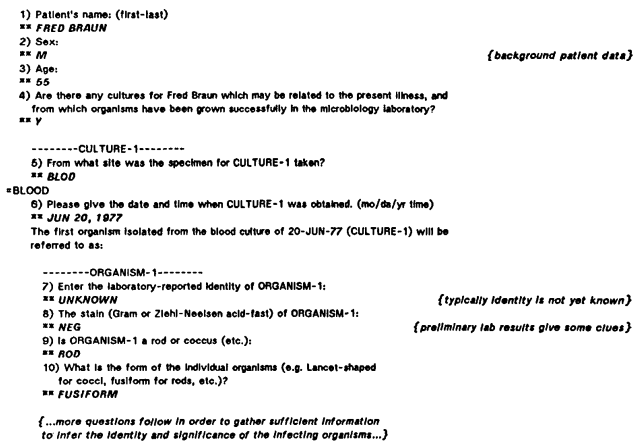
\includegraphics[width=4cm, trim={0 11cm 5.5cm 0},clip]{data/mycin.png}
            };
            \node[anchor=south east] at (mycin.north east) {MYCIN};

            \draw[gray, very thick, -Latex] ($ (interface.south) - (0.2, 0) $) to [out=270,in=0] ($ (db.west) + (0, 1.8) $) to [out=180,in=180] (db.west) {};
            \draw[gray, very thick, Latex-] ($ (interface.south) + (0.2, 0) $) to [out=270,in=180] ($ (db.east) + (0, 1.8) $) to [out=0,in=0] (db.east) {};

            \node[] (patient) at ($ (interface.north) + (0, 1.2) $) {
               \Huge{\emoji{face-with-thermometer}}
            };

            \draw[gray, very thick, Latex-Latex] (patient) -- (interface);

             \node[anchor=south, text depth=0] at ($ (db.west) + (0.6, 1.8) $) {\small{Data}};
             \node[anchor=south, text depth=0] at ($ (db.east) + (-0.6, 1.8) $) {\small{Prediksjon}};
             \node[] at (-4, 4.3) {};
             \node[] at (4, -3.45) {};

        \end{tikzpicture}
	\end{frame}

    \begin{frame}{Hva er kunstig intelligens?} % Symbolic: Doctor
        \centering
        \begin{tikzpicture}
            \node[draw=black, minimum height=4.6cm, minimum width=7cm, fill=blue!10] (mycin) at (0, 0) {};
            \node[draw=black, minimum height=2.2cm, minimum width=4cm, dashed] (db) at ($ (mycin) - (0, 0.7) $) {};
            \node[anchor=south, font=\small] at (db.north) {Kunnskapsdatabase};

            \node[draw=black, minimum width=2.4cm, anchor=south, fill=cyan!10] (fever) at ($ (db) + (0, 0.6) $) {FEBER > 39};
            \node[anchor=north] (and1) at (fever.south) {OG};
            \node[draw=black, anchor=north, minimum width=2.4cm, fill=cyan!10] (rod) at (and1.south) {BAKTERIE=STAV};
            \node[anchor=north] (and2) at (rod.south) {OG IKKE};
            \node[draw=black, anchor=north, minimum width=2.4cm, fill=cyan!10] (aerob) at (and2.south) {BAKTERIE=AEROB};

            \draw[gray, thick, -Latex] (db.west) to [out=0,in=180] (fever.west);
            \draw[gray, thick, -Latex] (db.west) to [out=0,in=180] (rod.west);
            \draw[gray, thick, -Latex] (db.west) to [out=0,in=180] (aerob.west);

            \draw[gray, thick, -Latex] (fever.east) to [out=0,in=180] (db.east);
            \draw[gray, thick, -Latex] (rod.east) to [out=0,in=180] (db.east);
            \draw[gray, thick, -Latex] (aerob.east) to [out=0,in=180] (db.east);

            \node[inner sep=0pt, draw=black] (interface) at (mycin.north) {
                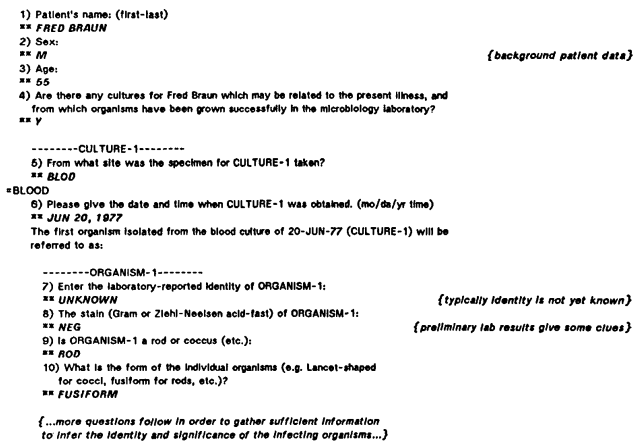
\includegraphics[width=4cm, trim={0 11cm 5.5cm 0},clip]{data/mycin.png}
            };
            \node[anchor=south east] at (mycin.north east) {MYCIN};

            \draw[gray, very thick, -Latex] ($ (interface.south) - (0.2, 0) $) to [out=270,in=0] ($ (db.west) + (0, 1.8) $) to [out=180,in=180] (db.west) {};
            \draw[gray, very thick, Latex-] ($ (interface.south) + (0.2, 0) $) to [out=270,in=180] ($ (db.east) + (0, 1.8) $) to [out=0,in=0] (db.east) {};

            \node[] (patient) at ($ (interface.north) + (0, 1.2) $) {
               \Huge{\emoji{face-with-thermometer}}
            };

            \draw[gray, very thick, Latex-Latex] (patient) -- (interface);

            \node[] (doctor) at ($ (mycin.south) - (0, 0.8) $) {
                \Huge{\emoji{health-worker}}
             };

             \node[anchor=south, text depth=0] at ($ (db.west) + (0.6, 1.8) $) {\small{Data}};
             \node[anchor=south, text depth=0] at ($ (db.east) + (-0.6, 1.8) $) {\small{Prediksjon}};

             \draw[gray, very thick, -Latex, dotted] (doctor) -- (db);
             \node[] at (-4, 4.3) {};
             \node[] at (4, -3.45) {};

        \end{tikzpicture}
	\end{frame}

    \begin{frame}{Hva er kunstig intelligens?} % Taxonomy: Symbolic
		\centering
		\vfill
		\begin{tikzpicture}
			\node[circle, fill=blue!60, minimum size=6cm] (ai) at (0, 0) {};
			\node[text=white, anchor=north] at ($ (ai.north) - (0, 0.3) $) {\textbf{Kunstig intelligens}};
			\node[text=white] at ($ (ai.north) - (-1.1, 1.2) $) {Symbolsk AI};
			\node[anchor=north west, align=left, font=\small] (ai-text) at ($ (ai.north) + (3.5, 0.0) $) {\textbf{Kunstig intelligens (AI):}\\Maskiner som løser problemer\\som krever intelligens};
			\node[] at (-3, 3) {};
			\node[] at (7.7, -3.2) {};
		\end{tikzpicture}
		\vfill
	\end{frame}

    \begin{frame}{Hva er kunstig intelligens?} % Taxonomy: ML
		\centering
		\vfill
		\begin{tikzpicture}
			\node[circle, fill=blue!60, minimum size=6cm] (ai) at (0, 0) {};
			\node[text=white, anchor=north] at ($ (ai.north) - (0, 0.3) $) {\textbf{Kunstig intelligens}};
			\node[text=white] at ($ (ai.north) - (-1.1, 1.2) $) {Symbolsk AI};
			\node[circle, fill=purple!60, minimum size=4.5cm, anchor=south] (ml) at ($ (ai.south) + (0, 0.05) $) {};
			\node[text=white, anchor=north] at ($ (ml.north) - (0, 0.3) $) {\textbf{Maskinlæring}};
			\node[anchor=north west, align=left, font=\small, text=gray!40] (ai-text) at ($ (ai.north) + (3.5, 0.0) $) {\textbf{Kunstig intelligens (AI):}\\Maskiner som løser problemer\\som krever intelligens};
			\node[anchor=north west, align=left, font=\small] (ml-text) at ($ (ai-text.south west) - (0, 0) $) {\textbf{Maskinlæring:}\\Maskiner som lærer å løse problemer\\gjennom å finne mønster i data};
			\node[] at (-3, 3) {};
			\node[] at (7.7, -3.2) {};
		\end{tikzpicture}
		\vfill
	\end{frame}

    \begin{frame}[t]{Hva er kunstig intelligens?} % ML: Symbolic
        \centering
        \begin{tikzpicture}
            \node[draw=black, minimum height=4.6cm, minimum width=7cm, fill=blue!10] (mycin) at (0, 0) {};
            \node[draw=black, minimum height=2.2cm, minimum width=4cm, dashed] (db) at ($ (mycin) - (0, 0.7) $) {};
            \node[anchor=south, font=\small] at (db.north) {Kunnskapsdatabase};

            \node[draw=black, minimum width=2.4cm, anchor=south, fill=cyan!10] (fever) at ($ (db) + (0, 0.6) $) {FEBER > 39};
            \node[anchor=north] (and1) at (fever.south) {OG};
            \node[draw=black, anchor=north, minimum width=2.4cm, fill=cyan!10] (rod) at (and1.south) {BAKTERIE=STAV};
            \node[anchor=north] (and2) at (rod.south) {OG IKKE};
            \node[draw=black, anchor=north, minimum width=2.4cm, fill=cyan!10] (aerob) at (and2.south) {BAKTERIE=AEROB};

            \draw[gray, thick, -Latex] (db.west) to [out=0,in=180] (fever.west);
            \draw[gray, thick, -Latex] (db.west) to [out=0,in=180] (rod.west);
            \draw[gray, thick, -Latex] (db.west) to [out=0,in=180] (aerob.west);

            \draw[gray, thick, -Latex] (fever.east) to [out=0,in=180] (db.east);
            \draw[gray, thick, -Latex] (rod.east) to [out=0,in=180] (db.east);
            \draw[gray, thick, -Latex] (aerob.east) to [out=0,in=180] (db.east);

            \node[inner sep=0pt, draw=black] (interface) at (mycin.north) {
                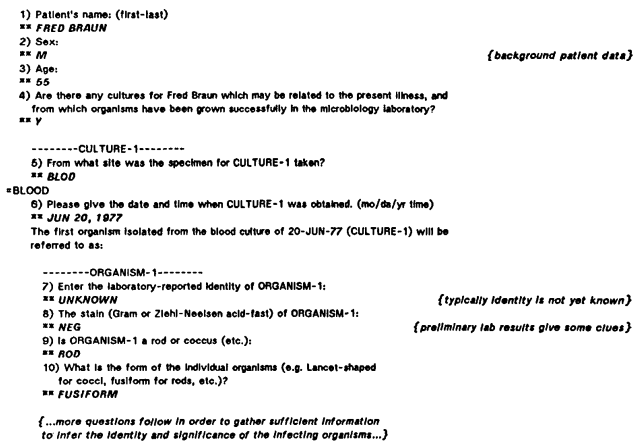
\includegraphics[width=4cm, trim={0 11cm 5.5cm 0},clip]{data/mycin.png}
            };
            \node[anchor=south east] at (mycin.north east) {MYCIN};

            \draw[gray, very thick, -Latex] ($ (interface.south) - (0.2, 0) $) to [out=270,in=0] ($ (db.west) + (0, 1.8) $) to [out=180,in=180] (db.west) {};
            \draw[gray, very thick, Latex-] ($ (interface.south) + (0.2, 0) $) to [out=270,in=180] ($ (db.east) + (0, 1.8) $) to [out=0,in=0] (db.east) {};

            \node[] (patient) at ($ (interface.north) + (0, 1.2) $) {
               \Huge{\emoji{face-with-thermometer}}
            };

            \draw[gray, very thick, Latex-Latex] (patient) -- (interface);

             \node[anchor=south, text depth=0] (input) at ($ (db.west) + (0.6, 1.8) $) {\small{Data}};
             \node[anchor=south, text depth=0] (output) at ($ (db.east) + (-0.6, 1.8) $) {\small{Prediksjon}};

             \node[] at (-5, 4.5) {};
             \node[] at (5, -2.6) {};

        \end{tikzpicture}
	\end{frame}

    \begin{frame}[t]{Hva er kunstig intelligens?} % ML: Predictive
        \centering
        \begin{tikzpicture}
            \node[minimum height=4.6cm, minimum width=7cm] (mycin) at (0, 0) {};
            \node[draw=black, minimum height=2.2cm, minimum width=4cm, fill=blue!10] (db) at ($ (mycin) - (0, 0.7) $) {};
            \node[anchor=south, font=\small] at (db.north) {Kunnskapsdatabase};

            \node[draw=black, minimum width=2.4cm, anchor=south, fill=cyan!10] (fever) at ($ (db) + (0, 0.6) $) {FEBER > 39};
            \node[anchor=north] (and1) at (fever.south) {OG};
            \node[draw=black, anchor=north, minimum width=2.4cm, fill=cyan!10] (rod) at (and1.south) {BAKTERIE=STAV};
            \node[anchor=north] (and2) at (rod.south) {OG IKKE};
            \node[draw=black, anchor=north, minimum width=2.4cm, fill=cyan!10] (aerob) at (and2.south) {BAKTERIE=AEROB};

            \draw[gray, thick, -Latex] (db.west) to [out=0,in=180] (fever.west);
            \draw[gray, thick, -Latex] (db.west) to [out=0,in=180] (rod.west);
            \draw[gray, thick, -Latex] (db.west) to [out=0,in=180] (aerob.west);

            \draw[gray, thick, -Latex] (fever.east) to [out=0,in=180] (db.east);
            \draw[gray, thick, -Latex] (rod.east) to [out=0,in=180] (db.east);
            \draw[gray, thick, -Latex] (aerob.east) to [out=0,in=180] (db.east);

             \node[anchor=east, text depth=0] (input) at ($ (db.west) - (1, 0) $) {\small{Data}};
             \node[anchor=west, text depth=0] (output) at ($ (db.east) + (1, 0) $) {\small{Prediksjon}};
             \node[] at (-5, 4.5) {};
             \node[] at (5, -2.6) {};

             \draw[gray, thick, -Latex] (input) -- (db.west);
             \draw[gray, thick, -Latex] (db.east) -- (output);

        \end{tikzpicture}
	\end{frame}

    \begin{frame}[t]{Hva er kunstig intelligens?} % ML: Model
        \centering
        \begin{tikzpicture}
            \node[minimum height=4.6cm, minimum width=7cm] (mycin) at (0, 0) {};
            \node[draw=black, minimum height=2.2cm, minimum width=4cm, fill=blue!10] (db) at ($ (mycin) - (0, 0.7) $) {};
            \node[anchor=south, font=\small] at (db.north) {Maskinlæringsmodell};

             \node[anchor=east, text depth=0] (input) at ($ (db.west) - (1, 0) $) {\small{Data}};
             \node[anchor=west, text depth=0] (output) at ($ (db.east) + (1, 0) $) {\small{Prediksjon}};
             \node[] at (-5, 4.5) {};
             \node[] at (5, -2.6) {};

             \draw[gray, thick, -Latex] (input) -- (db.west);
             \draw[gray, thick, -Latex] (db.east) -- (output);

        \end{tikzpicture}
	\end{frame}

    \begin{frame}[t]{Hva er kunstig intelligens?} % ML: Rules?
        \centering
        \begin{tikzpicture}
            \node[minimum height=4.6cm, minimum width=7cm] (mycin) at (0, 0) {};
            \node[draw=black, minimum height=2.2cm, minimum width=4cm, fill=blue!10] (db) at ($ (mycin) - (0, 0.7) $) {\Huge{?}};
            \node[anchor=south, font=\small] at (db.north) {Maskinlæringsmodell};

             \node[anchor=east, text depth=0] (input) at ($ (db.west) - (1, 0) $) {\small{Data}};
             \node[anchor=west, text depth=0] (output) at ($ (db.east) + (1, 0) $) {\small{Prediksjon}};
             \node[] at (-5, 4.5) {};
             \node[] at (5, -2.6) {};

             \draw[gray, thick, -Latex] (input) -- (db.west);
             \draw[gray, thick, -Latex] (db.east) -- (output);

        \end{tikzpicture}
	\end{frame}

    \begin{frame}[t]{Hva er kunstig intelligens?} % ML: Trees
        \centering
        \begin{tikzpicture}
            % Tree 1
            \node[] at (-3, 1) {
                {\fontsize{40}{48}\selectfont\emoji{deciduous-tree}}
            };
            % Tree 2
            \node[] at (-2, -1) {
                {\fontsize{50}{60}\selectfont\emoji{evergreen-tree}}
            };
            % Tree 3
            \node[] at (-1, 2) {
                {\fontsize{45}{54}\selectfont\emoji{deciduous-tree}}
            };
            % Tree 4
            \node[] at (0, -2) {
                {\fontsize{35}{42}\selectfont\emoji{evergreen-tree}}
            };
            % Tree 5
            \node[] at (1, 1) {
                {\fontsize{30}{36}\selectfont\emoji{deciduous-tree}}
            };
            % Tree 6
            \node[] at (2, -1) {
                {\fontsize{55}{66}\selectfont\emoji{evergreen-tree}}
            };
            % Tree 7
            \node[] at (3, 2) {
                {\fontsize{60}{72}\selectfont\emoji{deciduous-tree}}
            };
            % Tree 8
            \node[] at (-2.5, 0) {
                {\fontsize{38}{46}\selectfont\emoji{evergreen-tree}}
            };
            % Tree 9
            \node[] at (-1.5, -2) {
                {\fontsize{42}{50}\selectfont\emoji{deciduous-tree}}
            };
            % Tree 10
            \node[] at (0.5, 2) {
                {\fontsize{47}{56}\selectfont\emoji{evergreen-tree}}
            };
            % Tree 11
            \node[] at (1.5, -2.5) {
                {\fontsize{52}{62}\selectfont\emoji{deciduous-tree}}
            };
            % Tree 12
            \node[] at (2.5, 0) {
                {\fontsize{37}{44}\selectfont\emoji{evergreen-tree}}
            };
            % Tree 13
            \node[] at (-3, -2) {
                {\fontsize{43}{51}\selectfont\emoji{deciduous-tree}}
            };
            % Tree 14
            \node[] at (0, 0) {
                {\fontsize{48}{58}\selectfont\emoji{evergreen-tree}}
            };
            % Tree 15
            \node[] at (3, -2) {
                {\fontsize{33}{39}\selectfont\emoji{deciduous-tree}}
            };
        \end{tikzpicture}
	\end{frame}

    \begin{frame}[t]{Hva er kunstig intelligens?} % ML: Tree with age
        \centering
        \begin{tikzpicture}
            % Tree 1
            \node[] at (-3, 1) {
                {\fontsize{40}{48}\selectfont\emoji{deciduous-tree}}
            };
            % Tree 2
            \node[] at (-2, -1) {
                {\fontsize{50}{60}\selectfont\emoji{evergreen-tree}}
            };
            % Tree 3
            \node[label={[draw=black,fill=white]below:3.7 år}] at (-1, 2) {
                {\fontsize{45}{54}\selectfont\emoji{deciduous-tree}}
            };
            % Tree 4
            \node[] at (0, -2) {
                {\fontsize{35}{42}\selectfont\emoji{evergreen-tree}}
            };
            % Tree 5
            \node[] at (1, 1) {
                {\fontsize{30}{36}\selectfont\emoji{deciduous-tree}}
            };
            % Tree 6
            \node[] at (2, -1) {
                {\fontsize{55}{66}\selectfont\emoji{evergreen-tree}}
            };
            % Tree 7
            \node[] at (3, 2) {
                {\fontsize{60}{72}\selectfont\emoji{deciduous-tree}}
            };
            % Tree 8
            \node[] at (-2.5, 0) {
                {\fontsize{38}{46}\selectfont\emoji{evergreen-tree}}
            };
            % Tree 9
            \node[] at (-1.5, -2) {
                {\fontsize{42}{50}\selectfont\emoji{deciduous-tree}}
            };
            % Tree 10
            \node[] at (0.5, 2) {
                {\fontsize{47}{56}\selectfont\emoji{evergreen-tree}}
            };
            % Tree 11
            \node[] at (1.5, -2.5) {
                {\fontsize{52}{62}\selectfont\emoji{deciduous-tree}}
            };
            % Tree 12
            \node[] at (2.5, 0) {
                {\fontsize{37}{44}\selectfont\emoji{evergreen-tree}}
            };
            % Tree 13
            \node[] at (-3, -2) {
                {\fontsize{43}{51}\selectfont\emoji{deciduous-tree}}
            };
            % Tree 14
            \node[] at (0, 0) {
                {\fontsize{48}{58}\selectfont\emoji{evergreen-tree}}
            };
            % Tree 15
            \node[] at (3, -2) {
                {\fontsize{33}{39}\selectfont\emoji{deciduous-tree}}
            };
        \end{tikzpicture}
	\end{frame}

    \begin{frame}[t]{Hva er kunstig intelligens?} % ML: Ages
        \centering
        \begin{tikzpicture}
            % Tree 1
            \node[label={[draw=black,fill=white]below:3.3 år}] at (-3, 1) {
                {\fontsize{40}{48}\selectfont\emoji{deciduous-tree}}
            };
            % Tree 2
            \node[label={[draw=black,fill=white]below:4.1 år}] at (-2, -1) {
                {\fontsize{50}{60}\selectfont\emoji{evergreen-tree}}
            };
            % Tree 3
            \node[label={[draw=black,fill=white]below:3.7 år}] at (-1, 2) {
                {\fontsize{45}{54}\selectfont\emoji{deciduous-tree}}
            };
            % Tree 4
            \node[label={[draw=black,fill=white]below:2.9 år}] at (0, -2) {
                {\fontsize{35}{42}\selectfont\emoji{evergreen-tree}}
            };
            % Tree 5
            \node[label={[draw=black,fill=white]below:2.5 år}] at (1, 1) {
                {\fontsize{30}{36}\selectfont\emoji{deciduous-tree}}
            };
            % Tree 6
            \node[label={[draw=black,fill=white]below:4.5 år}] at (2, -1) {
                {\fontsize{55}{66}\selectfont\emoji{evergreen-tree}}
            };
            % Tree 7
            \node[label={[draw=black,fill=white]below:5 år}] at (3, 2) {
                {\fontsize{60}{72}\selectfont\emoji{deciduous-tree}}
            };
            % Tree 8
            \node[label={[draw=black,fill=white]below:3.1 år}] at (-2.5, 0) {
                {\fontsize{38}{46}\selectfont\emoji{evergreen-tree}}
            };
            % Tree 9
            \node[label={[draw=black,fill=white]below:3.5 år}] at (-1.5, -2) {
                {\fontsize{42}{50}\selectfont\emoji{deciduous-tree}}
            };
            % Tree 10
            \node[label={[draw=black,fill=white]below:3.9 år}] at (0.5, 2) {
                {\fontsize{47}{56}\selectfont\emoji{evergreen-tree}}
            };
            % Tree 11
            \node[label={[draw=black,fill=white]below:4.3 år}] at (1.5, -2.5) {
                {\fontsize{52}{62}\selectfont\emoji{deciduous-tree}}
            };
            % Tree 12
            \node[label={[draw=black,fill=white]below:3.0 år}] at (2.5, 0) {
                {\fontsize{37}{44}\selectfont\emoji{evergreen-tree}}
            };
            % Tree 13
            \node[label={[draw=black,fill=white]below:3.5 år}] at (-3, -2) {
                {\fontsize{43}{51}\selectfont\emoji{deciduous-tree}}
            };
            % Tree 14
            \node[label={[draw=black,fill=white]below:4 år}] at (0, 0) {
                {\fontsize{48}{58}\selectfont\emoji{evergreen-tree}}
            };
            % Tree 15
            \node[label={[draw=black,fill=white]below:2.7 år}] at (3, -2) {
                {\fontsize{33}{39}\selectfont\emoji{deciduous-tree}}
            };
        \end{tikzpicture}
	\end{frame}

    \begin{frame}{Hva er kunstig intelligens?} % ML: Ages
        \def\factor{30}
        \centering
        \begin{tikzpicture}
            % Tree 1
            \node[anchor=south, inner sep=0pt] at (0.4*\factor, 0) {
                {\fontsize{40}{48}\selectfont\emoji{deciduous-tree}}
            };
            % Tree 2
            \node[anchor=south, inner sep=0pt] at (0.5*\factor, 0) {
                {\fontsize{50}{60}\selectfont\emoji{evergreen-tree}}
            };
            % Tree 3
            \node[anchor=south, inner sep=0pt] at (0.45*\factor, 0) {
                {\fontsize{45}{54}\selectfont\emoji{deciduous-tree}}
            };
            % Tree 4
            \node[anchor=south, inner sep=0pt] at (0.35*\factor, 0) {
                {\fontsize{35}{42}\selectfont\emoji{evergreen-tree}}
            };
            % Tree 5
            \node[anchor=south, inner sep=0pt] at (0.3*\factor, 0) {
                {\fontsize{30}{36}\selectfont\emoji{deciduous-tree}}
            };
            % Tree 6
            \node[anchor=south, inner sep=0pt] at (0.55*\factor, 0) {
                {\fontsize{55}{66}\selectfont\emoji{evergreen-tree}}
            };
            % Tree 7
            \node[anchor=south, inner sep=0pt] at (0.6*\factor, 0) {
                {\fontsize{60}{72}\selectfont\emoji{deciduous-tree}}
            };
            % Tree 8
            \node[anchor=south, inner sep=0pt] at (0.38*\factor, 0) {
                {\fontsize{38}{46}\selectfont\emoji{evergreen-tree}}
            };
            % Tree 9
            \node[anchor=south, inner sep=0pt] at (0.42*\factor, 0) {
                {\fontsize{42}{50}\selectfont\emoji{deciduous-tree}}
            };
            % Tree 10
            \node[anchor=south, inner sep=0pt] at (0.47*\factor, 0) {
                {\fontsize{47}{56}\selectfont\emoji{evergreen-tree}}
            };
            % Tree 11
            \node[anchor=south, inner sep=0pt] at (0.52*\factor, 0) {
                {\fontsize{52}{62}\selectfont\emoji{deciduous-tree}}
            };
            % Tree 12
            \node[anchor=south, inner sep=0pt] at (0.37*\factor, 0) {
                {\fontsize{37}{44}\selectfont\emoji{evergreen-tree}}
            };
            % Tree 13
            \node[anchor=south, inner sep=0pt] at (0.43*\factor, 0) {
                {\fontsize{43}{51}\selectfont\emoji{deciduous-tree}}
            };
            % Tree 14
            \node[anchor=south, inner sep=0pt] at (0.48*\factor, 0) {
                {\fontsize{48}{58}\selectfont\emoji{evergreen-tree}}
            };
            % Tree 15
            \node[anchor=south, inner sep=0pt] at (0.33*\factor, 0) {
                {\fontsize{33}{39}\selectfont\emoji{deciduous-tree}}
            };

            \draw[thick] (0.28*\factor, -0.3) -- (0.62*\factor, -0.3);

            \node[anchor=north] at (0.45*\factor, -0.3) {Alder};
            \node[inner sep=1pt, fill=black, circle] at (0.4*\factor, -0.3) {};
            \node[inner sep=1pt, fill=black, circle] at (0.5*\factor, -0.3) {};
            \node[inner sep=1pt, fill=black, circle] at (0.45*\factor, -0.3) {};
            \node[inner sep=1pt, fill=black, circle] at (0.35*\factor, -0.3) {};
            \node[inner sep=1pt, fill=black, circle] at (0.3*\factor, -0.3) {};
            \node[inner sep=1pt, fill=black, circle] at (0.55*\factor, -0.3) {};
            \node[inner sep=1pt, fill=black, circle] at (0.6*\factor, -0.3) {};
            \node[inner sep=1pt, fill=black, circle] at (0.38*\factor, -0.3) {};
            \node[inner sep=1pt, fill=black, circle] at (0.42*\factor, -0.3) {};
            \node[inner sep=1pt, fill=black, circle] at (0.47*\factor, -0.3) {};
            \node[inner sep=1pt, fill=black, circle] at (0.52*\factor, -0.3) {};
            \node[inner sep=1pt, fill=black, circle] at (0.37*\factor, -0.3) {};
            \node[inner sep=1pt, fill=black, circle] at (0.43*\factor, -0.3) {};
            \node[inner sep=1pt, fill=black, circle] at (0.48*\factor, -0.3) {};
            \node[inner sep=1pt, fill=black, circle] at (0.33*\factor, -0.3) {};

            \node[] at (8, 3) {};
            \node[] at (19, -2) {};

        \end{tikzpicture}
	\end{frame}

    \begin{frame}{Hva er kunstig intelligens?} % ML: Ages
        \def\factor{30}
        \centering
        \begin{tikzpicture}
            % Tree 1
            \node[anchor=south, opacity=0.25, inner sep=0pt] (t0) at (0.4*\factor, 0) {
                {\fontsize{40}{48}\selectfont\emoji{deciduous-tree}}
            };
            % Tree 2
            \node[anchor=south, opacity=0.25, inner sep=0pt] (t1) at (0.5*\factor, 0) {
                {\fontsize{50}{60}\selectfont\emoji{evergreen-tree}}
            };
            % Tree 3
            \node[anchor=south, opacity=0.25, inner sep=0pt] (t2) at (0.45*\factor, 0) {
                {\fontsize{45}{54}\selectfont\emoji{deciduous-tree}}
            };
            % Tree 4
            \node[anchor=south, opacity=0.25, inner sep=0pt] (t3) at (0.35*\factor, 0) {
                {\fontsize{35}{42}\selectfont\emoji{evergreen-tree}}
            };
            % Tree 5
            \node[anchor=south, opacity=0.25, inner sep=0pt] (t4) at (0.3*\factor, 0) {
                {\fontsize{30}{36}\selectfont\emoji{deciduous-tree}}
            };
            % Tree 6
            \node[anchor=south, opacity=0.25, inner sep=0pt] (t5) at (0.55*\factor, 0) {
                {\fontsize{55}{66}\selectfont\emoji{evergreen-tree}}
            };
            % Tree 7
            \node[anchor=south, opacity=0.25, inner sep=0pt] (t6) at (0.6*\factor, 0) {
                {\fontsize{60}{72}\selectfont\emoji{deciduous-tree}}
            };
            % Tree 8
            \node[anchor=south, opacity=0.25, inner sep=0pt] (t7) at (0.38*\factor, 0) {
                {\fontsize{38}{46}\selectfont\emoji{evergreen-tree}}
            };
            % Tree 9
            \node[anchor=south, opacity=0.25, inner sep=0pt] (t8) at (0.42*\factor, 0) {
                {\fontsize{42}{50}\selectfont\emoji{deciduous-tree}}
            };
            % Tree 10
            \node[anchor=south, opacity=0.25, inner sep=0pt] (t9) at (0.47*\factor, 0) {
                {\fontsize{47}{56}\selectfont\emoji{evergreen-tree}}
            };
            % Tree 11
            \node[anchor=south, opacity=0.25, inner sep=0pt] (t10) at (0.52*\factor, 0) {
                {\fontsize{52}{62}\selectfont\emoji{deciduous-tree}}
            };
            % Tree 12
            \node[anchor=south, opacity=0.25, inner sep=0pt] (t11) at (0.37*\factor, 0) {
                {\fontsize{37}{44}\selectfont\emoji{evergreen-tree}}
            };
            % Tree 13
            \node[anchor=south, opacity=0.25, inner sep=0pt] (t12) at (0.43*\factor, 0) {
                {\fontsize{43}{51}\selectfont\emoji{deciduous-tree}}
            };
            % Tree 14
            \node[anchor=south, opacity=0.25, inner sep=0pt] (t13) at (0.48*\factor, 0) {
                {\fontsize{48}{58}\selectfont\emoji{evergreen-tree}}
            };
            % Tree 15
            \node[anchor=south, opacity=0.25, inner sep=0pt] (t14) at (0.33*\factor, 0) {
                {\fontsize{33}{39}\selectfont\emoji{deciduous-tree}}
            };

            \draw[thick] (0.28*\factor, -0.3) -- (0.62*\factor, -0.3);
            \draw[thick] (0.28*\factor, -0.3) -- (0.28*\factor, 2.5);

            \draw[gray] (t4.north) -- (t6.north);

            \node[anchor=north] at (0.45*\factor, -0.3) {Alder};
            \node[inner sep=1pt, fill=black, circle] at (t0.north) {};
            \node[inner sep=1pt, fill=black, circle] at (t1.north) {};
            \node[inner sep=1pt, fill=black, circle] at (t2.north) {};
            \node[inner sep=1pt, fill=black, circle] at (t3.north) {};
            \node[inner sep=1pt, fill=black, circle] at (t4.north) {};
            \node[inner sep=1pt, fill=black, circle] at (t5.north) {};
            \node[inner sep=1pt, fill=black, circle] at (t6.north) {};
            \node[inner sep=1pt, fill=black, circle] at (t7.north) {};
            \node[inner sep=1pt, fill=black, circle] at (t8.north) {};
            \node[inner sep=1pt, fill=black, circle] at (t9.north) {};
            \node[inner sep=1pt, fill=black, circle] at (t10.north) {};
            \node[inner sep=1pt, fill=black, circle] at (t11.north) {};
            \node[inner sep=1pt, fill=black, circle] at (t12.north) {};
            \node[inner sep=1pt, fill=black, circle] at (t13.north) {};
            \node[inner sep=1pt, fill=black, circle] at (t14.north) {};

            \node[rotate=90, anchor=south] at (0.28*\factor, 1.1) {Høyde};

            \node[] at (8, 3) {};
            \node[] at (19, -2) {};

        \end{tikzpicture}
	\end{frame}

    \begin{frame}{Hva er kunstig intelligens?} % ML: Ages
        \def\factor{30}
        \centering
        \begin{tikzpicture}
            % Tree 1
            \node[anchor=south, opacity=0.25, inner sep=0pt] (t0) at (0.4*\factor, 0) {
                {\fontsize{40}{48}\selectfont\emoji{deciduous-tree}}
            };
            % Tree 2
            \node[anchor=south, opacity=0.25, inner sep=0pt] (t1) at (0.5*\factor, 0) {
                {\fontsize{50}{60}\selectfont\emoji{evergreen-tree}}
            };
            % Tree 3
            \node[anchor=south, opacity=0.25, inner sep=0pt] (t2) at (0.45*\factor, 0) {
                {\fontsize{45}{54}\selectfont\emoji{deciduous-tree}}
            };
            % Tree 4
            \node[anchor=south, opacity=0.25, inner sep=0pt] (t3) at (0.35*\factor, 0) {
                {\fontsize{35}{42}\selectfont\emoji{evergreen-tree}}
            };
            % Tree 5
            \node[anchor=south, opacity=0.25, inner sep=0pt] (t4) at (0.3*\factor, 0) {
                {\fontsize{30}{36}\selectfont\emoji{deciduous-tree}}
            };
            % Tree 6
            \node[anchor=south, opacity=0.25, inner sep=0pt] (t5) at (0.55*\factor, 0) {
                {\fontsize{55}{66}\selectfont\emoji{evergreen-tree}}
            };
            % Tree 7
            \node[anchor=south, opacity=0.25, inner sep=0pt] (t6) at (0.6*\factor, 0) {
                {\fontsize{60}{72}\selectfont\emoji{deciduous-tree}}
            };
            % Tree 8
            \node[anchor=south, opacity=0.25, inner sep=0pt] (t7) at (0.38*\factor, 0) {
                {\fontsize{38}{46}\selectfont\emoji{evergreen-tree}}
            };
            % Tree 9
            \node[anchor=south, opacity=0.25, inner sep=0pt] (t8) at (0.42*\factor, 0) {
                {\fontsize{42}{50}\selectfont\emoji{deciduous-tree}}
            };
            % Tree 10
            \node[anchor=south, opacity=0.25, inner sep=0pt] (t9) at (0.47*\factor, 0) {
                {\fontsize{47}{56}\selectfont\emoji{evergreen-tree}}
            };
            % Tree 11
            \node[anchor=south, opacity=0.25, inner sep=0pt] (t10) at (0.52*\factor, 0) {
                {\fontsize{52}{62}\selectfont\emoji{deciduous-tree}}
            };
            % Tree 12
            \node[anchor=south, opacity=0.25, inner sep=0pt] (t11) at (0.37*\factor, 0) {
                {\fontsize{37}{44}\selectfont\emoji{evergreen-tree}}
            };
            % Tree 13
            \node[anchor=south, opacity=0.25, inner sep=0pt] (t12) at (0.43*\factor, 0) {
                {\fontsize{43}{51}\selectfont\emoji{deciduous-tree}}
            };
            % Tree 14
            \node[anchor=south, opacity=0.25, inner sep=0pt] (t13) at (0.48*\factor, 0) {
                {\fontsize{48}{58}\selectfont\emoji{evergreen-tree}}
            };
            % Tree 15
            \node[anchor=south, opacity=0.25, inner sep=0pt] (t14) at (0.33*\factor, 0) {
                {\fontsize{33}{39}\selectfont\emoji{deciduous-tree}}
            };

            \draw[thick] (0.28*\factor, -0.3) -- (0.62*\factor, -0.3);
            \draw[thick] (0.28*\factor, -0.3) -- (0.28*\factor, 2.5);

            \draw[gray] (t4.north) -- (t6.north);

            \node[anchor=north] at (0.45*\factor, -0.3) {Alder};
            \node[inner sep=1pt, fill=black, circle] at (t0.north) {};
            \node[inner sep=1pt, fill=black, circle] at (t1.north) {};
            \node[inner sep=1pt, fill=black, circle] at (t2.north) {};
            \node[inner sep=1pt, fill=black, circle] at (t3.north) {};
            \node[inner sep=1pt, fill=black, circle] at (t4.north) {};
            \node[inner sep=1pt, fill=black, circle] at (t5.north) {};
            \node[inner sep=1pt, fill=black, circle] at (t6.north) {};
            \node[inner sep=1pt, fill=black, circle] at (t7.north) {};
            \node[inner sep=1pt, fill=black, circle] at (t8.north) {};
            \node[inner sep=1pt, fill=black, circle] at (t9.north) {};
            \node[inner sep=1pt, fill=black, circle] at (t10.north) {};
            \node[inner sep=1pt, fill=black, circle] at (t11.north) {};
            \node[inner sep=1pt, fill=black, circle] at (t12.north) {};
            \node[inner sep=1pt, fill=black, circle] at (t13.north) {};
            \node[inner sep=1pt, fill=black, circle] at (t14.north) {};

            \node[rotate=90, anchor=south] at (0.28*\factor, 1.1) {Høyde};

            \node[] at (0.45*\factor, -1.5) {høyde$=0.5 + 1.2 *$alder};

            \node[] at (8, 3) {};
            \node[] at (19, -2) {};

        \end{tikzpicture}
	\end{frame}

    \begin{frame}[t]{Hva er kunstig intelligens?} % ML: Model math
        \centering
        \begin{tikzpicture}
            \node[minimum height=4.6cm, minimum width=7cm] (mycin) at (0, 0) {};
            \node[draw=black, minimum height=2.2cm, minimum width=4cm, fill=blue!10] (db) at ($ (mycin) - (0, 0.7) $) {$y=0.5+1.2*x$};
            \node[anchor=south, font=\small] at (db.north) {Maskinlæringsmodell};

             \node[anchor=east, text depth=0] (input) at ($ (db.west) - (1, 0) $) {\small{Data}};
             \node[anchor=west, text depth=0] (output) at ($ (db.east) + (1, 0) $) {\small{Prediksjon}};
             \node[] at (-5, 4.5) {};
             \node[] at (5, -2.6) {};

             \draw[gray, thick, -Latex] (input) -- (db.west);
             \draw[gray, thick, -Latex] (db.east) -- (output);

        \end{tikzpicture}
	\end{frame}

    \begin{frame}[t]{Hva er kunstig intelligens?} % Taxonomy: ML
		\centering
		\vfill
		\begin{tikzpicture}
			\node[circle, fill=blue!60, minimum size=6cm] (ai) at (0, 0) {};
			\node[text=white, anchor=north] at ($ (ai.north) - (0, 0.3) $) {\textbf{Kunstig intelligens}};
			\node[text=white] at ($ (ai.north) - (-1.1, 1.2) $) {Symbolsk AI};
			\node[circle, fill=purple!60, minimum size=4.5cm, anchor=south] (ml) at ($ (ai.south) + (0, 0.05) $) {};
			\node[text=white, anchor=north] at ($ (ml.north) - (0, 0.3) $) {\textbf{Maskinlæring}};
			\node[text=white, align=center, font=\linespread{0.5}\selectfont] at ($ (ml.north) - (1, 1.1) $) {Lineær\\regresjon};
			\node[anchor=north west, align=left, font=\small, text=gray!40] (ai-text) at ($ (ai.north) + (3.5, 0.0) $) {\textbf{Kunstig intelligens (AI):}\\Maskiner som løser problemer\\som krever intelligens};
			\node[anchor=north west, align=left, font=\small] (ml-text) at ($ (ai-text.south west) - (0, 0) $) {\textbf{Maskinlæring:}\\Maskiner som lærer å løse problemer\\gjennom å finne mønster i data};
			\node[] at (-3, 3) {};
			\node[] at (7.7, -3.2) {};
		\end{tikzpicture}
		\vfill
	\end{frame}

    \begin{frame}[t]{Hva er kunstig intelligens?} % Taxonomy: DL
		\centering
		\vfill
		\begin{tikzpicture}
			\node[circle, fill=blue!60, minimum size=6cm] (ai) at (0, 0) {};
			\node[text=white, anchor=north] at ($ (ai.north) - (0, 0.3) $) {\textbf{Kunstig intelligens}};
			\node[text=white] at ($ (ai.north) - (-1.1, 1.2) $) {Symbolsk AI};
			\node[circle, fill=purple!60, minimum size=4.5cm, anchor=south] (ml) at ($ (ai.south) + (0, 0.05) $) {};
			\node[text=white, anchor=north] at ($ (ml.north) - (0, 0.3) $) {\textbf{Maskinlæring}};
			\node[text=white, align=center, font=\linespread{0.5}\selectfont] at ($ (ml.north) - (1, 1.1) $) {Lineær\\regresjon};
			\node[circle, fill=red!60, minimum size=3cm, anchor=south] (dl) at ($ (ai.south) + (0, 0.1) $) {};
			\node[text=white, anchor=north] at ($ (dl.north) - (0, 0.3) $) {\textbf{Dyplæring}};
			\node[anchor=north west, align=left, font=\small, text=gray!40] (ai-text) at ($ (ai.north) + (3.5, 0.0) $) {\textbf{Kunstig intelligens (AI):}\\Maskiner som løser problemer\\som krever intelligens};
			\node[anchor=north west, align=left, font=\small, text=gray!40] (ml-text) at ($ (ai-text.south west) - (0, 0) $) {\textbf{Maskinlæring:}\\Maskiner som lærer å løse problemer\\gjennom å finne mønster i data};
			\node[anchor=north west, align=left, font=\small] (dl-text) at ($ (ml-text.south west) - (0, 0) $) {\textbf{Dyplæring:}\\Maskinlæringsmodeller som er\\hierarkisk organisert ($\approx$ dype\\nevrale nettverk), inspirert av\\hjernens struktur};
			\node[] at (-3, 3) {};
			\node[] at (7.7, -3.2) {};
		\end{tikzpicture}
		\vfill
	\end{frame}

    \begin{frame}[t]{Hva er kunstig intelligens?} % DL: ML
        \centering
        \begin{tikzpicture}
            \node[minimum height=4.6cm, minimum width=7cm] (mycin) at (0, 0) {};
            \node[draw=black, minimum height=2.5cm, minimum width=4cm, fill=blue!10] (db) at ($ (mycin) - (0, 0.7) $) {$y=0.5+1.2*x$};
            \node[anchor=south, font=\small] at (db.north) {Maskinlæringsmodell};

             \node[anchor=east, text depth=0] (input) at ($ (db.west) - (1, 0) $) {\small{Data}};
             \node[anchor=west, text depth=0] (output) at ($ (db.east) + (1, 0) $) {\small{Prediksjon}};
             \node[] at (-5, 4.5) {};
             \node[] at (5, -2.6) {};

             \draw[gray, thick, -Latex] (input) -- (db.west);
             \draw[gray, thick, -Latex] (db.east) -- (output);

        \end{tikzpicture}
	\end{frame}

    \begin{frame}[t]{Hva er kunstig intelligens?} % DL: DNN
        \centering
        \begin{tikzpicture}
            \node[minimum height=4.6cm, minimum width=7cm] (mycin) at (0, 0) {};
            \node[draw=black, minimum height=2.5cm, minimum width=4cm, fill=blue!10] (db) at ($ (mycin) - (0, 0.7) $) {};
            \node[anchor=south, font=\small] at (db.north) {Maskinlæringsmodell};

             \node[anchor=east, text depth=0] (input) at ($ (db.west) - (1, 0) $) {\small{Data}};
             \node[anchor=west, text depth=0] (output) at ($ (db.east) + (1, 0) $) {\small{Prediksjon}};


             \draw[gray, thick, -Latex] (input) -- (db.west);
             \draw[gray, thick, -Latex] (db.east) -- (output);

             \node[] at (-5, 4.5) {};
             \node[] at (5, -2.6) {};
             \node[inner sep=0pt, minimum size=0.4cm, draw=black, circle, fill=nodefill] (n00) at ($ (db) + (-1.5, -1) $) {};
             \node[inner sep=0pt, minimum size=0.4cm, draw=black, circle, fill=nodefill] (n01) at ($ (n00) + (0, 0.5) $) {};
             \node[inner sep=0pt, minimum size=0.4cm, draw=black, circle, fill=nodefill] (n02) at ($ (n00) + (0, 1.0) $) {};
             \node[inner sep=0pt, minimum size=0.4cm, draw=black, circle, fill=nodefill] (n03) at ($ (n00) + (0, 1.5) $) {};
             \node[inner sep=0pt, minimum size=0.4cm, draw=black, circle, fill=nodefill] (n04) at ($ (n00) + (0, 2.0) $) {};

             \node[inner sep=0pt, minimum size=0.4cm, draw=black, circle, fill=nodefill] (n10) at ($ (n00) + (0.75, 0.25) $) {};
             \node[inner sep=0pt, minimum size=0.4cm, draw=black, circle, fill=nodefill] (n11) at ($ (n00) + (0.75, 0.75) $) {};
             \node[inner sep=0pt, minimum size=0.4cm, draw=black, circle, fill=nodefill] (n12) at ($ (n00) + (0.75, 1.25) $) {};
             \node[inner sep=0pt, minimum size=0.4cm, draw=black, circle, fill=nodefill] (n13) at ($ (n00) + (0.75, 1.75) $) {};

             \node[inner sep=0pt, minimum size=0.4cm, draw=black, circle, fill=nodefill] (n20) at ($ (n00) + (1.5, 0.5) $) {};
             \node[inner sep=0pt, minimum size=0.4cm, draw=black, circle, fill=nodefill] (n21) at ($ (n00) + (1.5, 1.0) $) {};
             \node[inner sep=0pt, minimum size=0.4cm, draw=black, circle, fill=nodefill] (n22) at ($ (n00) + (1.5, 1.5) $) {};

             \node[inner sep=0pt, minimum size=0.4cm, draw=black, circle, fill=nodefill] (n30) at ($ (n00) + (2.25, 0.75) $) {};
             \node[inner sep=0pt, minimum size=0.4cm, draw=black, circle, fill=nodefill] (n31) at ($ (n00) + (2.25, 1.25) $) {};

             \node[inner sep=0pt, minimum size=0.4cm, draw=black, circle, fill=nodefill, text depth=0] (n40) at ($ (n00) + (3, 1.0) $) {};

             \draw[-] (db.west) -- (n00);
             \draw[-] (db.west) -- (n01);
             \draw[-] (db.west) -- (n02);
             \draw[-] (db.west) -- (n03);
             \draw[-] (db.west) -- (n04);
             \draw[-] (db.west) -- (n00);
             \draw[-] (db.west) -- (n01);
             \draw[-] (db.west) -- (n02);
             \draw[-] (db.west) -- (n03);
             \draw[-] (db.west) -- (n04);
             \draw[-] (db.west) -- (n00);
             \draw[-] (db.west) -- (n01);
             \draw[-] (db.west) -- (n02);
             \draw[-] (db.west) -- (n03);
             \draw[-] (db.west) -- (n04);

             \draw[-] (n00) -- (n10);
             \draw[-] (n00) -- (n11);
             \draw[-] (n00) -- (n12);
             \draw[-] (n00) -- (n13);
             \draw[-] (n01) -- (n10);
             \draw[-] (n01) -- (n11);
             \draw[-] (n01) -- (n12);
             \draw[-] (n01) -- (n13);
             \draw[-] (n02) -- (n10);
             \draw[-] (n02) -- (n11);
             \draw[-] (n02) -- (n12);
             \draw[-] (n02) -- (n13);
             \draw[-] (n03) -- (n10);
             \draw[-] (n03) -- (n11);
             \draw[-] (n03) -- (n12);
             \draw[-] (n03) -- (n13);
             \draw[-] (n04) -- (n10);
             \draw[-] (n04) -- (n11);
             \draw[-] (n04) -- (n12);
             \draw[-] (n04) -- (n13);

             \draw[-] (n10) -- (n20);
             \draw[-] (n10) -- (n21);
             \draw[-] (n10) -- (n22);
             \draw[-] (n11) -- (n20);
             \draw[-] (n11) -- (n21);
             \draw[-] (n11) -- (n22);
             \draw[-] (n12) -- (n20);
             \draw[-] (n12) -- (n21);
             \draw[-] (n12) -- (n22);
             \draw[-] (n13) -- (n20);
             \draw[-] (n13) -- (n21);
             \draw[-] (n13) -- (n22);

             \draw[-] (n20) -- (n30);
             \draw[-] (n20) -- (n31);
             \draw[-] (n21) -- (n30);
             \draw[-] (n21) -- (n31);
             \draw[-] (n22) -- (n30);
             \draw[-] (n22) -- (n31);

             \draw[-] (n30) -- (n40);
             \draw[-] (n31) -- (n40);

             \draw[-] (n40) -- (db.east);

        \end{tikzpicture}
	\end{frame}

    \begin{frame}{Hva er kunstig intelligens?} % Taxonomy, CNNs and LLMs
		\centering
		\vfill
		\begin{tikzpicture}
			\node[circle, fill=blue!60, minimum size=6cm] (ai) at (0, 0) {};
			\node[text=white, anchor=north] at ($ (ai.north) - (0, 0.3) $) {\textbf{Kunstig intelligens}};
			\node[text=white] at ($ (ai.north) - (-1.1, 1.2) $) {Symbolsk AI};
			\node[circle, fill=purple!60, minimum size=4.5cm, anchor=south] (ml) at ($ (ai.south) + (0, 0.05) $) {};
			\node[text=white, anchor=north] at ($ (ml.north) - (0, 0.3) $) {\textbf{Maskinlæring}};
			\node[text=white, align=center, font=\linespread{0.5}\selectfont] at ($ (ml.north) - (1, 1.1) $) {Lineær\\regresjon};
			\node[circle, fill=red!60, minimum size=3cm, anchor=south] (dl) at ($ (ai.south) + (0, 0.1) $) {};
			\node[text=white, anchor=north] at ($ (dl.north) - (0, 0.3) $) {\textbf{Dyplæring}};
			\node[anchor=north west, align=left, font=\small, text=gray!40] (ai-text) at ($ (ai.north) + (3.5, 0.0) $) {\textbf{Kunstig intelligens (AI):}\\Maskiner som løser problemer\\som krever intelligens};
			\node[anchor=north west, align=left, font=\small, text=gray!40] (ml-text) at ($ (ai-text.south west) - (0, 0) $) {\textbf{Maskinlæring:}\\Maskiner som lærer å løse problemer\\gjennom å finne mønster i data};
			\node[anchor=north west, align=left, font=\small] (dl-text) at ($ (ml-text.south west) - (0, 0) $) {\textbf{Dyplæring:}\\Maskinlæringsmodeller som er\\hierarkisk organisert ($\approx$ dype\\nevrale nettverk), inspirert av\\hjernens struktur};
			\node[] at (-3, 3) {};
			\node[] at (7.7, -3.2) {};
		\end{tikzpicture}
		\vfill
	\end{frame}

    \begin{frame}{Hva er kunstig intelligens?} % Taxonomy, CNNs and LLMs
		\centering
		\vfill
		\begin{tikzpicture}
			\node[circle, fill=blue!60, minimum size=6cm] (ai) at (0, 0) {};
			\node[text=white, anchor=north] at ($ (ai.north) - (0, 0.3) $) {\textbf{Kunstig intelligens}};
			\node[text=white] at ($ (ai.north) - (-1.1, 1.2) $) {Symbolsk AI};
			\node[circle, fill=purple!60, minimum size=4.5cm, anchor=south] (ml) at ($ (ai.south) + (0, 0.05) $) {};
			\node[text=white, anchor=north] at ($ (ml.north) - (0, 0.3) $) {\textbf{Maskinlæring}};
			\node[text=white, align=center, font=\linespread{0.5}\selectfont] at ($ (ml.north) - (1, 1.1) $) {Lineær\\regresjon};
			\node[circle, fill=red!60, minimum size=3cm, anchor=south] (dl) at ($ (ai.south) + (0, 0.1) $) {};
			\node[text=white, anchor=north] at ($ (dl.north) - (0, 0.3) $) {\textbf{Dyplæring}};
			\node[align=center, text=white, font=\linespread{0.5}\selectfont] at ($ (dl.north) - (-0.2, 1.2) $) {Konvolusjonelle\\nevral nettverk};
			\node[align=center, text=white, font=\linespread{0.5}\selectfont] at ($ (dl.north) - (0.2, 2.1) $) {Store\\språkmodeller};
			\node[anchor=north west, align=left, font=\small, text=gray!40] (ai-text) at ($ (ai.north) + (3.5, 0.0) $) {\textbf{Kunstig intelligens (AI):}\\Maskiner som løser problemer\\som krever intelligens};
			\node[anchor=north west, align=left, font=\small, text=gray!40] (ml-text) at ($ (ai-text.south west) - (0, 0) $) {\textbf{Maskinlæring:}\\Maskiner som lærer å løse problemer\\gjennom å finne mønster i data};
			\node[anchor=north west, align=left, font=\small, text=gray!40] (dl-text) at ($ (ml-text.south west) - (0, 0) $) {\textbf{Dyplæring:}\\Maskinlæringsmodeller som er\\hierarkisk organisert ($\approx$ dype\\nevrale nettverk), inspirert av\\hjernens struktur};
			\node[anchor=north west, align=left, font=\small] (cnn-text) at ($ (dl-text.south west) - (0, 0) $) {\textbf{Konvolusjonelle nevrale nettverk:}\\Nevrale nettverk for prosessering\\av bildedata};
			\node[anchor=north west, align=left, font=\small] at ($ (cnn-text.south west) - (0, 0) $) {\textbf{Store språkmodeller:}\\(Store) nevrale nettverk\\for språkprosessering (ChatGPT)};
			\node[] at (-3, 3) {};
			\node[] at (7.7, -3.2) {};
		\end{tikzpicture}
		\vfill
	\end{frame}

    \begin{frame}{Terminologi: Veiledet vs ikke-veiledet læring} % Supervised vs unsupervised
		\centering
		\vfill
		\begin{tikzpicture}
			\node[align=center, anchor=north] (supervised) at (0, 0) {Veiledet læring\\(Supervised learning)};
			\node[align=center, anchor=north] (unsupervised) at (7, 0) {Ikke-veiledet læring\\(Unsupervised learning)};
			\draw[] (3.5, 0) -- (3.5, -7.5);
			\node[] (cat1) at ($ (supervised.south) + (-1, -0.8) $) {
				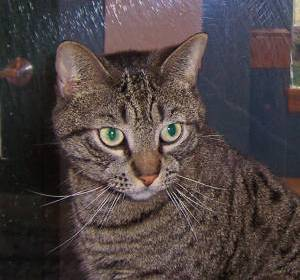
\includegraphics[width=1.2cm]{data/cat.1.jpg}
			};
			\node[anchor=west] (cattext1) at ($ (cat1.east) + (1.2, 0) $) {Katt};
			\draw[->] (cat1) -- (cattext1);
			\node[anchor=north] (dog1) at ($ (cat1.south) + (0, -0.1) $) {
				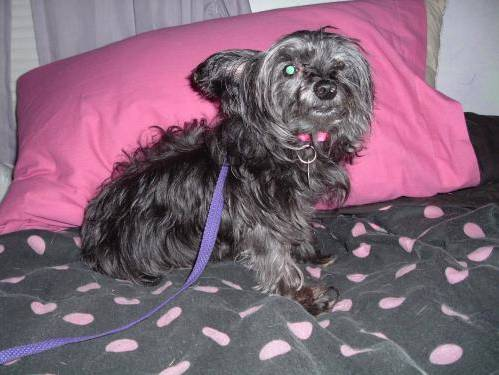
\includegraphics[width=1.2cm]{data/dog.0.jpg}
			};
			\node[anchor=west] (dogtext1) at ($ (dog1.east) + (1.2, 0) $) {Hund};
			\draw[->] (dog1) -- (dogtext1);
			\node[anchor=north] (cat2) at ($ (dog1.south) + (0, -0.1) $) {
				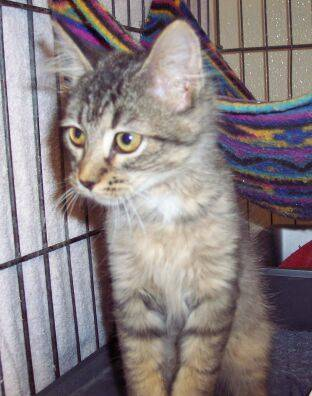
\includegraphics[width=1.2cm]{data/cat.2.jpg}
			};
			\node[anchor=west] (cattext2) at ($ (cat2.east) + (1.2, 0) $) {Katt};
			\draw[->] (cat2) -- (cattext2);
			\node[anchor=north] (dog2) at ($ (cat2.south) + (0, -0.1) $) {
				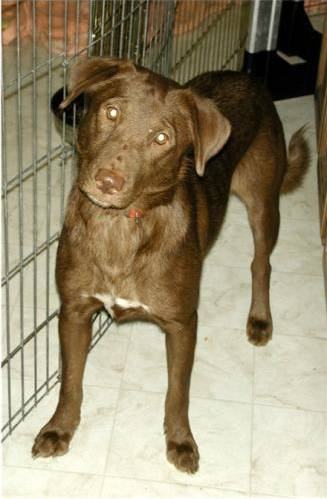
\includegraphics[width=1.2cm]{data/dog.1.jpg}
			};
			\node[anchor=west] (dogtext2) at ($ (dog2.east) + (1.2, 0) $) {Hund};
			\draw[->] (dog2) -- (dogtext2);

			\node[] (cat1) at ($ (unsupervised.south) + (-1.2, -1.1) $) {
				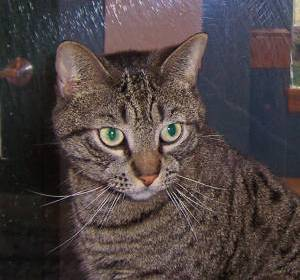
\includegraphics[width=0.8cm]{data/cat.1.jpg}
			};
			\node[] (cat2) at ($ (cat1) + (-0.9, 0.2) $) {
				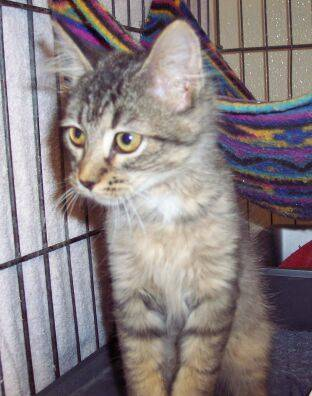
\includegraphics[width=0.8cm]{data/cat.2.jpg}
			};
			\node[] (cat3) at ($ (cat1) + (-0.5, -0.8) $) {
				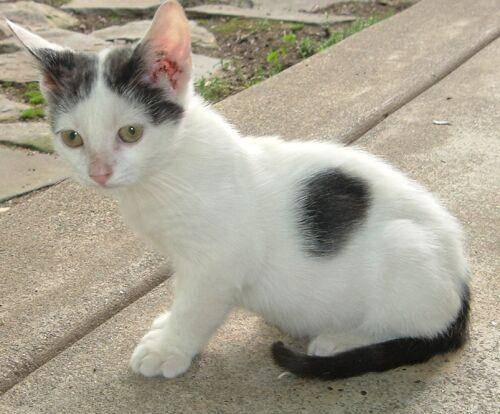
\includegraphics[width=0.8cm]{data/cat.3.jpg}
			};
			\node[] (cat4) at ($ (cat1) + (0.9, -0.1) $) {
				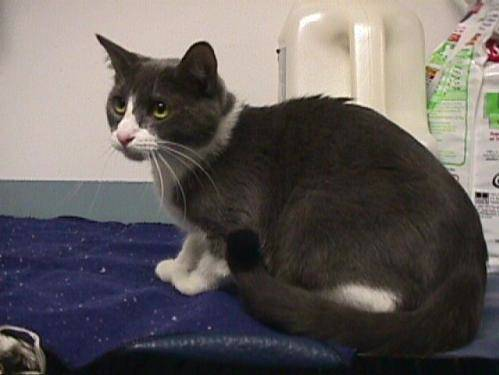
\includegraphics[width=0.8cm]{data/cat.4.jpg}
			};

			\node[] (dog1) at ($ (cat1) + (1.8, -1.5) $) {
				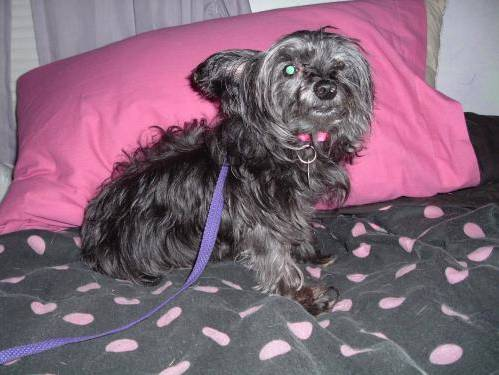
\includegraphics[width=0.8cm]{data/dog.0.jpg}
			};
			\node[] (dog2) at ($ (dog1) + (0.9, 0.1) $) {
				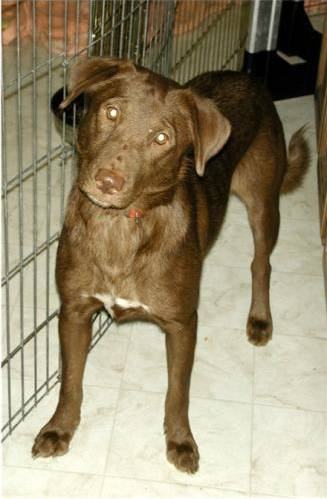
\includegraphics[width=0.8cm]{data/dog.1.jpg}
			};
			\node[] (dog3) at ($ (dog1) + (0.3, -0.8) $) {
				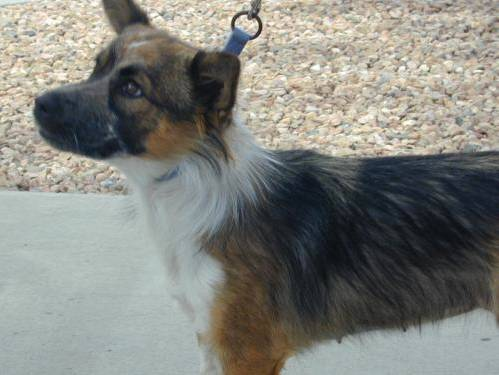
\includegraphics[width=0.8cm]{data/dog.3.jpg}
			};
			\node[] (dog4) at ($ (dog1) + (-0.9, -0.3) $) {
				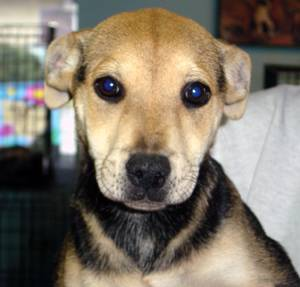
\includegraphics[width=0.8cm]{data/dog.4.jpg}
			};
			\draw[dashed, thick, red] ($ (cat1) + (-0.9, -1.7) $) -- ($ (dog1) + (1.2, 1.7) $);
		\end{tikzpicture}
		\vfill
	\end{frame}

    % \section{Kunstig intelligens i medisinsk forskning}

    % \begin{frame}{AI i medisinsk forskning}
    %     \centering
    %     \begin{tikzpicture}
    %         \node[] {
    %             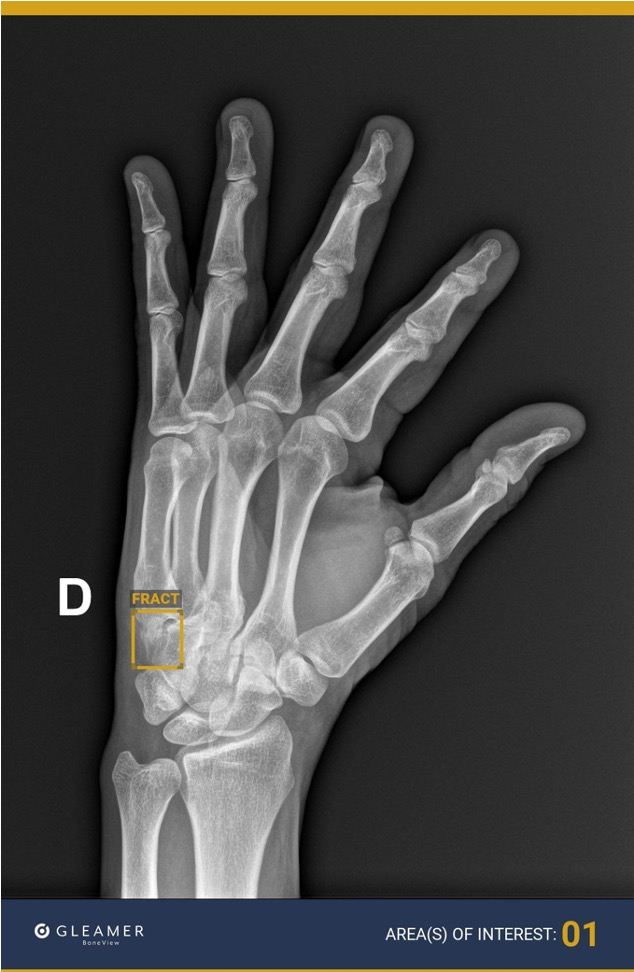
\includegraphics[width=4cm]{data/gleamer.jpeg}
    %         };
    %     \end{tikzpicture}
    % \end{frame}

    % \begin{frame}{AI i hjerneforskning: Presisjonsdiagnostikk} % MRI
    %     \centering
    %     \begin{tikzpicture}
    %         \node[inner sep=0pt] (c0) at (-1.6, 0) {
    %             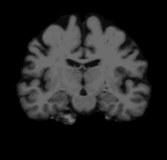
\includegraphics[width=3cm]{data/control_0.png}
    %         };

    %         \node[] at (-3, 2.1) {};
    %         \node[] at (7, -5.6) {};
    %         \node[anchor=east] at (8.7, -5.6) {
    %             \footnotesize{Data fra Open Access Series of Imaging Studies 3 (OASIS-3)}
    %         };
    %     \end{tikzpicture}
    % \end{frame}

    % \begin{frame}{AI i hjerneforskning: Presisjonsdiagnostikk} % Case-control
    %     \centering
    %     \begin{tikzpicture}
    %         \node[inner sep=0pt, draw=green, very thick] (c0) at (-1.6, 0) {
    %             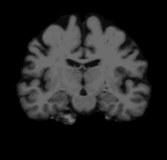
\includegraphics[width=3cm]{data/control_0.png}
    %         };
    %         \node[inner sep=0pt, draw=green, very thick] (c1) at (4, 0) {
    %             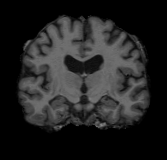
\includegraphics[width=3cm]{data/control_1.png}
    %         };
    %         \node[inner sep=0pt, draw=red, very thick] (p0) at (-1.6, -3.5) {
    %             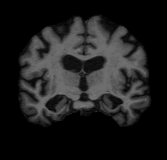
\includegraphics[width=3cm]{data/patient_0.png}
    %         };
    %         \node[inner sep=0pt, draw=red, very thick] (p1) at (4, -3.5) {
    %             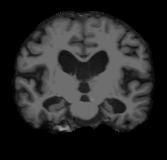
\includegraphics[width=3cm]{data/patient_1.png}
    %         };

    %         \node[anchor=south west, align=left] at (p0.south east) {
    %             Pasient
    %         };

    %         \node[anchor=south west, align=left] at (p1.south east) {
    %             Pasient
    %         };

    %         \node[anchor=south west, align=left] at (c0.south east) {
    %             Frisk
    %         };

    %         \node[anchor=south west, align=left] at (c1.south east) {
    %             Frisk
    %         };

    %         \node[] at (-3, 2.1) {};
    %         \node[] at (7, -5.6) {};
    %         \node[anchor=east] at (8.7, -5.6) {
    %             \footnotesize{Data fra Open Access Series of Imaging Studies 3 (OASIS-3)}
    %         };
    %     \end{tikzpicture}
    % \end{frame}

    % \begin{frame}{AI i hjerneforskning: Presisjonsdiagnostikk} % Hippocampus
    %     \centering
    %     \begin{tikzpicture}
    %         \node[inner sep=0pt, draw=green, very thick] (c0) at (-1.6, 0) {
    %             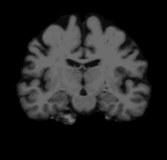
\includegraphics[width=3cm]{data/control_0.png}
    %         };
    %         \node[inner sep=0pt, draw=green, very thick] (c1) at (4, 0) {
    %             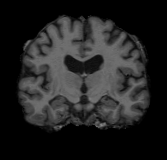
\includegraphics[width=3cm]{data/control_1.png}
    %         };
    %         \node[inner sep=0pt, draw=red, very thick] (p0) at (-1.6, -3.5) {
    %             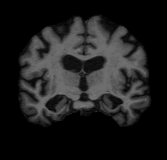
\includegraphics[width=3cm]{data/patient_0.png}
    %         };
    %         \node[inner sep=0pt, draw=red, very thick] (p1) at (4, -3.5) {
    %             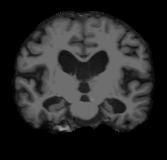
\includegraphics[width=3cm]{data/patient_1.png}
    %         };

    %         \node[anchor=south west, align=left] at (p0.south east) {
    %             Pasient
    %         };

    %         \node[anchor=south west, align=left] at (p1.south east) {
    %             Pasient
    %         };

    %         \node[anchor=south west, align=left] at (c0.south east) {
    %             Frisk
    %         };

    %         \node[anchor=south west, align=left] at (c1.south east) {
    %             Frisk
    %         };

    %         \draw[red, thick] ($ (p0.south east) + (-1.05, 1.07) $) circle (0.26cm);
    %         \draw[red, thick] ($ (p0.south east) + (-1.98, 1.03) $) circle (0.27cm);

    %         \draw[red, thick] ($ (p1.south east) + (-1.02, 1) $) circle (0.29cm);
    %         \draw[red, thick] ($ (p1.south east) + (-2.02, 1.04) $) circle (0.29cm);

    %         \draw[green, thick] ($ (c1.south east) + (-1.07, 1.05) $) circle (0.25cm);
    %         \draw[green, thick] ($ (c1.south east) + (-1.97, 1.05) $) circle (0.25cm);

    %         \draw[green, thick] ($ (c0.south east) + (-1.07, 1.15) $) circle (0.25cm);
    %         \draw[green, thick] ($ (c0.south east) + (-1.97, 1.15) $) circle (0.25cm);

    %         \node[] at (-3, 2.1) {};
    %         \node[] at (7, -5.6) {};
    %         \node[anchor=east] at (8.7, -5.6) {
    %             \footnotesize{Data fra Open Access Series of Imaging Studies 3 (OASIS-3)}
    %         };
    %     \end{tikzpicture}
    % \end{frame}

    % \begin{frame}{AI i hjerneforskning: Presisjonsdiagnostikk} % Nuances
    %     \centering
    %     \begin{tikzpicture}
    %         \node[inner sep=0pt, draw=green, very thick] (c0) at (-1.6, 0) {
    %             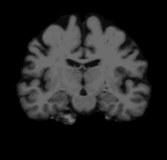
\includegraphics[width=3cm]{data/control_0.png}
    %         };
    %         \node[inner sep=0pt, draw=green, very thick] (c1) at (4, 0) {
    %             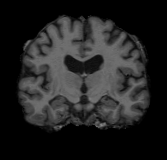
\includegraphics[width=3cm]{data/control_1.png}
    %         };
    %         \node[inner sep=0pt, draw=red, very thick] (p0) at (-1.6, -3.5) {
    %             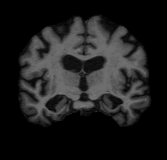
\includegraphics[width=3cm]{data/patient_0.png}
    %         };
    %         \node[inner sep=0pt, draw=red, very thick] (p1) at (4, -3.5) {
    %             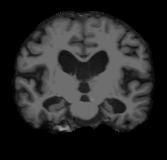
\includegraphics[width=3cm]{data/patient_1.png}
    %         };

    %         \node[anchor=south west, align=left] at (p0.south east) {
    %             \textcolor{gray!50}{Ikke effektivt}\\
    %             Talevansker\\
    %             Pasient
    %         };

    %         \node[anchor=south west, align=left] at (p1.south east) {
    %             \textcolor{gray!50}{Effektivt}\\
    %             Hukommelsessvikt\\
    %             Pasient
    %         };

    %         \node[anchor=south west, align=left] at (c0.south east) {
    %             Frisk
    %         };

    %         \node[anchor=south west, align=left] at (c1.south east) {
    %             Frisk
    %         };

    %         \draw[red, thick] ($ (p0.south east) + (-1.05, 1.07) $) circle (0.26cm);
    %         \draw[red, thick] ($ (p0.south east) + (-1.98, 1.03) $) circle (0.27cm);

    %         \draw[red, thick] ($ (p1.south east) + (-1.02, 1) $) circle (0.29cm);
    %         \draw[red, thick] ($ (p1.south east) + (-2.02, 1.04) $) circle (0.29cm);

    %         \draw[green, thick] ($ (c1.south east) + (-1.07, 1.05) $) circle (0.25cm);
    %         \draw[green, thick] ($ (c1.south east) + (-1.97, 1.05) $) circle (0.25cm);

    %         \draw[green, thick] ($ (c0.south east) + (-1.07, 1.15) $) circle (0.25cm);
    %         \draw[green, thick] ($ (c0.south east) + (-1.97, 1.15) $) circle (0.25cm);

    %         \node[] at (-3, 2.1) {};
    %         \node[] at (7, -5.6) {};
    %         \node[anchor=east] at (8.7, -5.6) {
    %             \footnotesize{Data fra Open Access Series of Imaging Studies 3 (OASIS-3)}
    %         };
    %     \end{tikzpicture}
    % \end{frame}

    % \begin{frame}{AI i hjerneforskning: Presisjonsdiagnostikk} % Patient ventricles
    %     \centering
    %     \begin{tikzpicture}
    %         \node[inner sep=0pt, draw=green, very thick] (c0) at (-1.6, 0) {
    %             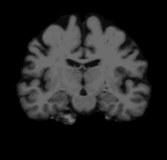
\includegraphics[width=3cm]{data/control_0.png}
    %         };
    %         \node[inner sep=0pt, draw=green, very thick] (c1) at (4, 0) {
    %             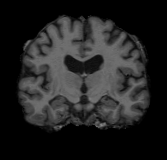
\includegraphics[width=3cm]{data/control_1.png}
    %         };
    %         \node[inner sep=0pt, draw=red, very thick] (p0) at (-1.6, -3.5) {
    %             \includegraphics[width=3cm]{data/patient_0.png}
    %         };
    %         \node[inner sep=0pt, draw=red, very thick] (p1) at (4, -3.5) {
    %             \includegraphics[width=3cm]{data/patient_1.png}
    %         };

    %         \node[anchor=south west, align=left] at (p0.south east) {
    %             \textcolor{gray!50}{Ikke effektivt}\\
    %             Talevansker\\
    %             Pasient
    %         };

    %         \node[anchor=south west, align=left] at (p1.south east) {
    %             \textcolor{gray!50}{Effektivt}\\
    %             Hukommelsessvikt\\
    %             Pasient
    %         };

    %         \node[anchor=south west, align=left] at (c0.south east) {
    %             Frisk
    %         };

    %         \node[anchor=south west, align=left] at (c1.south east) {
    %             Frisk
    %         };

    %         \draw[red, thick, opacity=0.25] ($ (p0.south east) + (-1.05, 1.07) $) circle (0.26cm);
    %         \draw[red, thick, opacity=0.25] ($ (p0.south east) + (-1.98, 1.03) $) circle (0.27cm);

    %         \draw[red, thick, opacity=0.25] ($ (p1.south east) + (-1.02, 1) $) circle (0.29cm);
    %         \draw[red, thick, opacity=0.25] ($ (p1.south east) + (-2.02, 1.04) $) circle (0.29cm);

    %         \draw[green, thick, opacity=0.25] ($ (c1.south east) + (-1.07, 1.05) $) circle (0.25cm);
    %         \draw[green, thick, opacity=0.25] ($ (c1.south east) + (-1.97, 1.05) $) circle (0.25cm);

    %         \draw[green, thick, opacity=0.25] ($ (c0.south east) + (-1.07, 1.15) $) circle (0.25cm);
    %         \draw[green, thick, opacity=0.25] ($ (c0.south east) + (-1.97, 1.15) $) circle (0.25cm);

    %         \draw[orange, thick] ($ (p0.north west) + (1, -0.95) $) rectangle ($ (p0.north east) - (1, 1.4) $);
    %         \draw[orange, thick] ($ (p1.north west) + (0.95, -0.85) $) rectangle ($ (p1.north east) - (0.95, 1.5) $);

    %         \node[] at (-3, 2.1) {};
    %         \node[] at (7, -5.6) {};
    %         \node[anchor=east] at (8.7, -5.6) {
    %             \footnotesize{Data fra Open Access Series of Imaging Studies 3 (OASIS-3)}
    %         };
    %     \end{tikzpicture}
    % \end{frame}

    % \begin{frame}{AI i hjerneforskning: Presisjonsdiagnostikk} % Healthy ventricles
    %     \centering
    %     \begin{tikzpicture}
    %         \node[inner sep=0pt, draw=green, very thick] (c0) at (-1.6, 0) {
    %             \includegraphics[width=3cm]{data/control_0.png}
    %         };
    %         \node[inner sep=0pt, draw=green, very thick] (c1) at (4, 0) {
    %             \includegraphics[width=3cm]{data/control_1.png}
    %         };
    %         \node[inner sep=0pt, draw=red, very thick] (p0) at (-1.6, -3.5) {
    %             \includegraphics[width=3cm]{data/patient_0.png}
    %         };
    %         \node[inner sep=0pt, draw=red, very thick] (p1) at (4, -3.5) {
    %             \includegraphics[width=3cm]{data/patient_1.png}
    %         };

    %         \node[anchor=south west, align=left] at (p0.south east) {
    %             \textcolor{gray!50}{Ikke effektivt}\\
    %             Talevansker\\
    %             Pasient
    %         };

    %         \node[anchor=south west, align=left] at (p1.south east) {
    %             \textcolor{gray!50}{Effektivt}\\
    %             Hukommelsessvikt\\
    %             Pasient
    %         };

    %         \node[anchor=south west, align=left] at (c0.south east) {
    %             Frisk
    %         };

    %         \node[anchor=south west, align=left] at (c1.south east) {
    %             Frisk
    %         };

    %         \draw[red, thick, opacity=0.25] ($ (p0.south east) + (-1.05, 1.07) $) circle (0.26cm);
    %         \draw[red, thick, opacity=0.25] ($ (p0.south east) + (-1.98, 1.03) $) circle (0.27cm);

    %         \draw[red, thick, opacity=0.25] ($ (p1.south east) + (-1.02, 1) $) circle (0.29cm);
    %         \draw[red, thick, opacity=0.25] ($ (p1.south east) + (-2.02, 1.04) $) circle (0.29cm);

    %         \draw[green, thick, opacity=0.25] ($ (c1.south east) + (-1.07, 1.05) $) circle (0.25cm);
    %         \draw[green, thick, opacity=0.25] ($ (c1.south east) + (-1.97, 1.05) $) circle (0.25cm);

    %         \draw[green, thick, opacity=0.25] ($ (c0.south east) + (-1.07, 1.15) $) circle (0.25cm);
    %         \draw[green, thick, opacity=0.25] ($ (c0.south east) + (-1.97, 1.15) $) circle (0.25cm);

    %         \draw[orange, thick] ($ (p0.north west) + (1, -0.95) $) rectangle ($ (p0.north east) - (1, 1.4) $);
    %         \draw[orange, thick] ($ (p1.north west) + (0.95, -0.85) $) rectangle ($ (p1.north east) - (0.95, 1.5) $);
    %         \draw[orange, thick] ($ (c1.north west) + (1.1, -0.95) $) rectangle ($ (c1.north east) - (1.1, 1.45) $);

    %         \node[] at (-3, 2.1) {};
    %         \node[] at (7, -5.6) {};
    %         \node[anchor=east] at (8.7, -5.6) {
    %             \footnotesize{Data fra Open Access Series of Imaging Studies 3 (OASIS-3)}
    %         };
    %     \end{tikzpicture}
    % \end{frame}

    % \begin{frame}{AI i hjerneforskning: Presisjonsdiagnostikk} % Cortex
    %     \centering
    %     \begin{tikzpicture}
    %         \node[inner sep=0pt, draw=green, very thick] (c0) at (-1.6, 0) {
    %             \includegraphics[width=3cm]{data/control_0.png}
    %         };
    %         \node[inner sep=0pt, draw=green, very thick] (c1) at (4, 0) {
    %             \includegraphics[width=3cm]{data/control_1.png}
    %         };
    %         \node[inner sep=0pt, draw=red, very thick] (p0) at (-1.6, -3.5) {
    %             \includegraphics[width=3cm]{data/patient_0.png}
    %         };
    %         \node[inner sep=0pt, draw=red, very thick] (p1) at (4, -3.5) {
    %             \includegraphics[width=3cm]{data/patient_1.png}
    %         };

    %         \node[anchor=south west, align=left] at (p0.south east) {
    %             \textcolor{gray!50}{Ikke effektivt}\\
    %             Talevansker\\
    %             Pasient
    %         };

    %         \node[anchor=south west, align=left] at (p1.south east) {
    %             \textcolor{gray!50}{Effektivt}\\
    %             Hukommelsessvikt\\
    %             Pasient
    %         };

    %         \node[anchor=south west, align=left] at (c0.south east) {
    %             Frisk
    %         };

    %         \node[anchor=south west, align=left] at (c1.south east) {
    %             Frisk
    %         };

    %         \draw[red, thick, opacity=0.25] ($ (p0.south east) + (-1.05, 1.07) $) circle (0.26cm);
    %         \draw[red, thick, opacity=0.25] ($ (p0.south east) + (-1.98, 1.03) $) circle (0.27cm);

    %         \draw[red, thick, opacity=0.25] ($ (p1.south east) + (-1.02, 1) $) circle (0.29cm);
    %         \draw[red, thick, opacity=0.25] ($ (p1.south east) + (-2.02, 1.04) $) circle (0.29cm);

    %         \draw[green, thick, opacity=0.25] ($ (c1.south east) + (-1.07, 1.05) $) circle (0.25cm);
    %         \draw[green, thick, opacity=0.25] ($ (c1.south east) + (-1.97, 1.05) $) circle (0.25cm);

    %         \draw[green, thick, opacity=0.25] ($ (c0.south east) + (-1.07, 1.15) $) circle (0.25cm);
    %         \draw[green, thick, opacity=0.25] ($ (c0.south east) + (-1.97, 1.15) $) circle (0.25cm);

    %         \draw[orange, thick, opacity=0.25] ($ (p0.north west) + (1, -0.95) $) rectangle ($ (p0.north east) - (1, 1.4) $);
    %         \draw[orange, thick, opacity=0.25] ($ (p1.north west) + (0.95, -0.85) $) rectangle ($ (p1.north east) - (0.95, 1.5) $);
    %         \draw[orange, thick, opacity=0.25] ($ (c1.north west) + (1.1, -0.95) $) rectangle ($ (c1.north east) - (1.1, 1.45) $);

    %         \draw[->, orange, thick] ($ (p0.north west) + (0.35, -0.35) $) -- ($ (p0.north west) + (0.7, -0.6) $);
    %         \draw[->, orange, thick] ($ (p0.north east) - (0.35, 0.35) $) -- ($ (p0.north east) - (0.65, 0.65) $);

    %         \draw[->, orange, thick] ($ (p1.north west) + (0.35, -0.35) $) -- ($ (p1.north west) + (0.7, -0.6) $);
    %         \draw[->, orange, thick] ($ (p1.north east) - (0.35, 0.27) $) -- ($ (p1.north east) - (0.7, 0.57) $);

    %         \node[] at (-3, 2.1) {};
    %         \node[] at (7, -5.6) {};
    %         \node[anchor=east] at (8.7, -5.6) {
    %             \footnotesize{Data fra Open Access Series of Imaging Studies 3 (OASIS-3)}
    %         };
    %     \end{tikzpicture}
    % \end{frame}

    % \begin{frame}{AI i hjerneforskning: Presisjonsdiagnostikk} % Everything
    %     \centering
    %     \begin{tikzpicture}
    %         \node[inner sep=0pt, draw=green, very thick] (c0) at (-1.6, 0) {
    %             \includegraphics[width=3cm]{data/control_0.png}
    %         };
    %         \node[inner sep=0pt, draw=green, very thick] (c1) at (4, 0) {
    %             \includegraphics[width=3cm]{data/control_1.png}
    %         };
    %         \node[inner sep=0pt, draw=red, very thick] (p0) at (-1.6, -3.5) {
    %             \includegraphics[width=3cm]{data/patient_0.png}
    %         };
    %         \node[inner sep=0pt, draw=red, very thick] (p1) at (4, -3.5) {
    %             \includegraphics[width=3cm]{data/patient_1.png}
    %         };

    %         \node[anchor=south west, align=left] at (p0.south east) {
    %             84 år\\
    %             Mann\\
    %             \textcolor{gray!50}{Ikke effektivt}\\
    %             Talevansker\\
    %             Pasient
    %         };

    %         \node[anchor=south west, align=left] at (p1.south east) {
    %             81 år\\
    %             Kvinne\\
    %             \textcolor{gray!50}{Effektivt}\\
    %             Hukommelsessvikt\\
    %             Pasient
    %         };

    %         \node[anchor=south west, align=left] at (c0.south east) {
    %             74 år\\
    %             Kvinne\\
    %             Frisk
    %         };

    %         \node[anchor=south west, align=left] at (c1.south east) {
    %             75 år\\
    %             Mann\\
    %             Frisk
    %         };

    %         \draw[red, thick] ($ (p0.south east) + (-1.05, 1.07) $) circle (0.26cm);
    %         \draw[red, thick] ($ (p0.south east) + (-1.98, 1.03) $) circle (0.27cm);

    %         \draw[red, thick] ($ (p1.south east) + (-1.02, 1) $) circle (0.29cm);
    %         \draw[red, thick] ($ (p1.south east) + (-2.02, 1.04) $) circle (0.29cm);

    %         \draw[green, thick] ($ (c1.south east) + (-1.07, 1.05) $) circle (0.25cm);
    %         \draw[green, thick] ($ (c1.south east) + (-1.97, 1.05) $) circle (0.25cm);

    %         \draw[green, thick] ($ (c0.south east) + (-1.07, 1.15) $) circle (0.25cm);
    %         \draw[green, thick] ($ (c0.south east) + (-1.97, 1.15) $) circle (0.25cm);

    %         \draw[orange, thick] ($ (p0.north west) + (1, -0.95) $) rectangle ($ (p0.north east) - (1, 1.4) $);
    %         \draw[orange, thick] ($ (p1.north west) + (0.95, -0.85) $) rectangle ($ (p1.north east) - (0.95, 1.5) $);
    %         \draw[orange, thick] ($ (c1.north west) + (1.1, -0.95) $) rectangle ($ (c1.north east) - (1.1, 1.45) $);

    %         \draw[->, orange, thick] ($ (p0.north west) + (0.35, -0.35) $) -- ($ (p0.north west) + (0.7, -0.6) $);
    %         \draw[->, orange, thick] ($ (p0.north east) - (0.35, 0.35) $) -- ($ (p0.north east) - (0.65, 0.65) $);

    %         \draw[->, orange, thick] ($ (p1.north west) + (0.35, -0.35) $) -- ($ (p1.north west) + (0.7, -0.6) $);
    %         \draw[->, orange, thick] ($ (p1.north east) - (0.35, 0.27) $) -- ($ (p1.north east) - (0.7, 0.57) $);

    %         \node[] at (-3, 2.1) {};
    %         \node[] at (7, -5.6) {};
    %         \node[anchor=east] at (8.7, -5.6) {
    %             \footnotesize{Data fra Open Access Series of Imaging Studies 3 (OASIS-3)}
    %         };
    %     \end{tikzpicture}
    % \end{frame}

    % \begin{frame}{AI i hjerneforskning: Presisjonsdiagnostikk} % Striked out
    %     \centering
    %     \begin{tikzpicture}
    %         \node[inner sep=0pt, draw=green, very thick] (c0) at (-1.6, 0) {
    %             \includegraphics[width=3cm]{data/control_0.png}
    %         };
    %         \node[inner sep=0pt, draw=green, very thick] (c1) at (4, 0) {
    %             \includegraphics[width=3cm]{data/control_1.png}
    %         };
    %         \node[inner sep=0pt, draw=red, very thick] (p0) at (-1.6, -3.5) {
    %             \includegraphics[width=3cm]{data/patient_0.png}
    %         };
    %         \node[inner sep=0pt, draw=red, very thick] (p1) at (4, -3.5) {
    %             \includegraphics[width=3cm]{data/patient_1.png}
    %         };

    %         \node[anchor=south west, align=left] at (p0.south east) {
    %             \sout{84 år}\\
    %             \sout{Mann}\\
    %             \textcolor{gray!50}{Ikke effektivt}\\
    %             Talevansker\\
    %             \sout{Pasient}
    %         };

    %         \node[anchor=south west, align=left] at (p1.south east) {
    %             \sout{81 år}\\
    %             \sout{Kvinne}\\
    %             \textcolor{gray!50}{Effektivt}\\
    %             Hukommelsessvikt\\
    %             \sout{Pasient}
    %         };

    %         \node[anchor=south west, align=left] at (c0.south east) {
    %             \sout{74 år}\\
    %             \sout{Kvinne}\\
    %             \sout{Frisk}
    %         };

    %         \node[anchor=south west, align=left] at (c1.south east) {
    %             \sout{75 år}\\
    %             \sout{Mann}\\
    %             \sout{Frisk}
    %         };

    %         \draw[red, thick] ($ (p0.south east) + (-1.05, 1.07) $) circle (0.26cm);
    %         \draw[red, thick] ($ (p0.south east) + (-1.98, 1.03) $) circle (0.27cm);

    %         \draw[red, thick] ($ (p1.south east) + (-1.02, 1) $) circle (0.29cm);
    %         \draw[red, thick] ($ (p1.south east) + (-2.02, 1.04) $) circle (0.29cm);

    %         \draw[green, thick] ($ (c1.south east) + (-1.07, 1.05) $) circle (0.25cm);
    %         \draw[green, thick] ($ (c1.south east) + (-1.97, 1.05) $) circle (0.25cm);

    %         \draw[green, thick] ($ (c0.south east) + (-1.07, 1.15) $) circle (0.25cm);
    %         \draw[green, thick] ($ (c0.south east) + (-1.97, 1.15) $) circle (0.25cm);

    %         \draw[orange, thick] ($ (p0.north west) + (1, -0.95) $) rectangle ($ (p0.north east) - (1, 1.4) $);
    %         \draw[orange, thick] ($ (p1.north west) + (0.95, -0.85) $) rectangle ($ (p1.north east) - (0.95, 1.5) $);
    %         \draw[orange, thick] ($ (c1.north west) + (1.1, -0.95) $) rectangle ($ (c1.north east) - (1.1, 1.45) $);

    %         \draw[->, orange, thick] ($ (p0.north west) + (0.35, -0.35) $) -- ($ (p0.north west) + (0.7, -0.6) $);
    %         \draw[->, orange, thick] ($ (p0.north east) - (0.35, 0.35) $) -- ($ (p0.north east) - (0.65, 0.65) $);

    %         \draw[->, orange, thick] ($ (p1.north west) + (0.35, -0.35) $) -- ($ (p1.north west) + (0.7, -0.6) $);
    %         \draw[->, orange, thick] ($ (p1.north east) - (0.35, 0.27) $) -- ($ (p1.north east) - (0.7, 0.57) $);

    %         \node[] at (-3, 2.1) {};
    %         \node[] at (7, -5.6) {};
    %         \node[anchor=east] at (8.7, -5.6) {
    %             \footnotesize{Data fra Open Access Series of Imaging Studies 3 (OASIS-3)}
    %         };
    %     \end{tikzpicture}
    % \end{frame}

    % \begin{frame}{AI i hjerneforskning: Presisjonsdiagnostikk} % Binary model
    %     \centering
    %     \vfill
	% 	\begin{tikzpicture}[scale=0.9]
    %         \newcommand{\mrivsep}{0.52}
	% 		\newcommand{\mrihsep}{0.44}
	% 		\def\plotwidth{11.68}

	% 		\newcommand{\nodesize}{11pt}
	% 		\newcommand{\hsep}{28pt}
	% 		\newcommand{\vsep}{14pt}

	% 		\newcommand{\arrowwidth}{0.05cm}
	% 		\newcommand{\innerarrow}{{Latex[length=0.1cm, width=0.15cm]}}
	% 		\newcommand{\outerarrow}{{Latex[length=0.2cm, width=0.3cm]}}

	% 		\definecolor{cb-green}{HTML}{4dac93}
	% 		\definecolor{cb-blue}{HTML}{3594d6}
	% 		\definecolor{outercolor}{RGB}{128, 128, 128}
	% 		\colorlet{train-fill}{cb-blue}

	% 		\newcommand{\patientlocation}[1]{($ (1, -1.6) + ####1 $)}
	% 		\newcommand{\controllocation}[1]{($ (1, -2.8) + ####1 $)}
	% 		\newcommand{\modellocation}[1]{($ (0.5 * \plotwidth, -2.2) + ####1 $)}

    %         \node[thick, draw=green, inner sep=0pt] (p0) at (2, -1.1) {
    %             \includegraphics[width=0.6cm]{data/samples/control_0.png}
    %         };

    %         \node[thick, draw=green, inner sep=0pt] (p0) at (1.1, -0.7) {
    %             \includegraphics[width=0.6cm]{data/samples/control_1.png}
    %         };

    %         \node[thick, draw=green, inner sep=0pt] (p0) at (1.25, -1.9) {
    %             \includegraphics[width=0.6cm]{data/samples/control_2.png}
    %         };

    %         \node[thick, draw=green, inner sep=0pt] (p0) at (0.3, -1.4) {
    %             \includegraphics[width=0.6cm]{data/samples/control_3.png}
    %         };

    %         \node[thick, draw=red, inner sep=0pt] (p0) at (2.2, -3.1) {
    %             \includegraphics[width=0.6cm]{data/samples/control_4.png}
    %         };

    %         \node[thick, draw=red, inner sep=0pt] (p0) at (1.4, -3.2) {
    %             \includegraphics[width=0.6cm]{data/samples/control_5.png}
    %         };

    %         \node[thick, draw=red, inner sep=0pt] (p0) at (0.4, -2.7) {
    %             \includegraphics[width=0.6cm]{data/samples/dementia_0.png}
    %         };

	% 		\node[circle, inner sep=0pt, fill=none, outer sep=0pt, line width=0pt, draw=none] (n00) at \modellocation{(-3 * \hsep, 0)} {};

	% 		\node[circle, minimum size=\nodesize, inner sep=0pt, fill=train-fill!35, outer sep=0pt, line width=0pt, draw=train-fill!35] (n10) at \modellocation{(-2 * \hsep, 2 * \vsep)} {};
	% 		\node[circle, minimum size=\nodesize, inner sep=0pt, fill=train-fill, outer sep=0pt, line width=0pt, draw=train-fill] (n11) at \modellocation{(-2 * \hsep, 1 * \vsep)} {};
	% 		\node[circle, minimum size=\nodesize, inner sep=0pt, fill=train-fill!15, outer sep=0pt, line width=0pt, draw=train-fill!15] (n12) at \modellocation{(-2 * \hsep, 0)} {};
	% 		\node[circle, minimum size=\nodesize, inner sep=0pt, fill=train-fill!85, outer sep=0pt, line width=0pt, draw=train-fill!85] (n13) at \modellocation{(-2 * \hsep, -1 * \vsep)} {};
	% 		\node[circle, minimum size=\nodesize, inner sep=0pt, fill=train-fill!90, outer sep=0pt, line width=0pt, draw=train-fill!90] (n14) at \modellocation{(-2 * \hsep, -2 * \vsep)} {};

	% 		\node[circle, minimum size=\nodesize, inner sep=0pt, fill=train-fill!55, outer sep=0pt, line width=0pt, draw=train-fill!55] (n20) at \modellocation{(-1 * \hsep, 1.5 * \vsep)} {};
	% 		\node[circle, minimum size=\nodesize, inner sep=0pt, fill=train-fill!20, outer sep=0pt, line width=0pt, draw=train-fill!20] (n21) at \modellocation{(-1 * \hsep, 0.5 * \vsep)} {};
	% 		\node[circle, minimum size=\nodesize, inner sep=0pt, fill=train-fill!90, outer sep=0pt, line width=0pt, draw=train-fill!50] (n22) at \modellocation{(-1 * \hsep, -0.5 * \vsep)} {};
	% 		\node[circle, minimum size=\nodesize, inner sep=0pt, fill=train-fill!35, outer sep=0pt, line width=0pt, draw=train-fill!35] (n23) at \modellocation{(-1 * \hsep, -1.5 * \vsep)} {};

	% 		\node[circle, minimum size=\nodesize, inner sep=0pt, fill=train-fill!95, outer sep=0pt, line width=0pt, draw=train-fill!65] (n30) at \modellocation{(0 * \hsep, 1.5 * \vsep)} {};
	% 		\node[circle, minimum size=\nodesize, inner sep=0pt, fill=train-fill!20, outer sep=0pt, line width=0pt, draw=train-fill!20] (n31) at \modellocation{(0 * \hsep, 0.5 * \vsep)} {};
	% 		\node[circle, minimum size=\nodesize, inner sep=0pt, fill=train-fill!90, outer sep=0pt, line width=0pt, draw=train-fill!90] (n32) at \modellocation{(0 * \hsep, -0.5 * \vsep)} {};
	% 		\node[circle, minimum size=\nodesize, inner sep=0pt, fill=train-fill!80, outer sep=0pt, line width=0pt, draw=train-fill!80] (n33) at \modellocation{(0 * \hsep, -1.5 * \vsep)} {};

	% 		\node[circle, minimum size=\nodesize, inner sep=0pt, fill=train-fill!50, outer sep=0pt, line width=0pt, draw=train-fill!50] (n40) at \modellocation{(1 * \hsep, 1*\vsep)} {};
	% 		\node[circle, minimum size=\nodesize, inner sep=0pt, fill=train-fill!90, outer sep=0pt, line width=0pt, draw=train-fill!70] (n41) at \modellocation{(1 * \hsep, 0*\vsep)} {};
	% 		\node[circle, minimum size=\nodesize, inner sep=0pt, fill=train-fill!70, outer sep=0pt, line width=0pt, draw=train-fill!30] (n42) at \modellocation{(1 * \hsep, -1*\vsep)} {};

	% 		\node[circle, minimum size=\nodesize, inner sep=0pt, fill=train-fill, outer sep=0pt, line width=0pt, draw=train-fill] (n50) at \modellocation{(2 * \hsep, 1*\vsep)} {};
	% 		\node[circle, minimum size=\nodesize, inner sep=0pt, fill=train-fill!70, outer sep=0pt, line width=0pt, draw=train-fill!70] (n51) at \modellocation{(2 * \hsep, 0*\vsep)} {};
	% 		\node[circle, minimum size=\nodesize, inner sep=0pt, fill=train-fill!30, outer sep=0pt, line width=0pt, draw=train-fill!30] (n52) at \modellocation{(2 * \hsep, -1*\vsep)} {};

	% 		\node[circle, minimum size=\nodesize, inner sep=0pt, fill=train-fill!80, outer sep=0pt, line width=0pt, draw=train-fill!65] (n60) at \modellocation{(3 * \hsep, 0)} {};

	% 		\draw[
	% 			color=train-fill!35,
	% 			-\innerarrow,
	% 			line width=\arrowwidth
	% 		] (n00) to [out=20,in=200] (n10) {};
	% 		\draw[
	% 			color=train-fill,
	% 			-\innerarrow,
	% 			line width=\arrowwidth
	% 		] (n00) to [out=10,in=190] (n11) {};
	% 		\draw[
	% 			color=train-fill!15,
	% 			-\innerarrow,
	% 			line width=\arrowwidth
	% 		] (n00) to [out=0,in=180] (n12) {};
	% 		\draw[
	% 			color=train-fill!85,
	% 			-\innerarrow,
	% 			line width=\arrowwidth
	% 		] (n00) to [out=-10,in=170] (n13) {};
	% 		\draw[
	% 			color=train-fill!90,
	% 			-\innerarrow,
	% 			line width=\arrowwidth
	% 		] (n00) to [out=-20,in=160] (n14) {};

	% 		\draw[
	% 			color=train-fill!35,
	% 			-\innerarrow,
	% 			line width=\arrowwidth
	% 		] (n10) to [out=-5,in=175] (n20) {};
	% 		\draw[
	% 			color=train-fill!10,
	% 			-\innerarrow,
	% 			line width=\arrowwidth
	% 		] (n10) to [out=-15,in=165] (n21) {};
	% 		\draw[
	% 			color=train-fill!70,
	% 			-\innerarrow,
	% 			line width=\arrowwidth
	% 		] (n10) to [out=-25,in=155] (n22) {};
	% 		\draw[
	% 			color=train-fill!50,
	% 			-\innerarrow,
	% 			line width=\arrowwidth
	% 		] (n10) to [out=-35,in=145] (n23) {};

	% 		\draw[
	% 			color=train-fill!30,
	% 			-\innerarrow,
	% 			line width=\arrowwidth
	% 		] (n11) to [out=5,in=185] (n20) {};
	% 		\draw[
	% 			color=train-fill!25,
	% 			-\innerarrow,
	% 			line width=\arrowwidth
	% 		] (n11) to [out=-5,in=175] (n21) {};
	% 		\draw[
	% 			color=train-fill!95,
	% 			-\innerarrow,
	% 			line width=\arrowwidth
	% 		] (n11) to [out=-15,in=165] (n22) {};
	% 		\draw[
	% 			color=train-fill!35,
	% 			-\innerarrow,
	% 			line width=\arrowwidth
	% 		] (n11) to [out=-25,in=155] (n23) {};

	% 		\draw[
	% 			color=train-fill!70,
	% 			-\innerarrow,
	% 			line width=\arrowwidth
	% 		] (n12) to [out=15,in=195] (n20) {};
	% 		\draw[
	% 			color=train-fill!20,
	% 			-\innerarrow,
	% 			line width=\arrowwidth
	% 		] (n12) to [out=5,in=185] (n21) {};
	% 		\draw[
	% 			color=train-fill!80,
	% 			-\innerarrow,
	% 			line width=\arrowwidth
	% 		] (n12) to [out=-5,in=175] (n22) {};
	% 		\draw[
	% 			color=train-fill,
	% 			-\innerarrow,
	% 			line width=\arrowwidth
	% 		] (n12) to [out=-15,in=165] (n23) {};

	% 		\draw[
	% 			color=train-fill!40,
	% 			-\innerarrow,
	% 			line width=\arrowwidth
	% 		] (n13) to [out=25,in=205] (n20) {};
	% 		\draw[
	% 			color=train-fill!35,
	% 			-\innerarrow,
	% 			line width=\arrowwidth
	% 		] (n13) to [out=15,in=195] (n21) {};
	% 		\draw[
	% 			color=train-fill!20,
	% 			-\innerarrow,
	% 			line width=\arrowwidth
	% 		] (n13) to [out=5,in=185] (n22) {};
	% 		\draw[
	% 			color=white,
	% 			-\innerarrow,
	% 			line width=\arrowwidth
	% 		] (n13) to [out=-5,in=175] (n23) {};

	% 		\draw[
	% 			color=train-fill!40,
	% 			-\innerarrow,
	% 			line width=\arrowwidth
	% 		] (n14) to [out=35,in=215] (n20) {};
	% 		\draw[
	% 			color=train-fill!85,
	% 			-\innerarrow,
	% 			line width=\arrowwidth
	% 		] (n14) to [out=25,in=205] (n21) {};
	% 		\draw[
	% 			color=train-fill!35,
	% 			-\innerarrow,
	% 			line width=\arrowwidth
	% 		] (n14) to [out=15,in=195] (n22) {};
	% 		\draw[
	% 			color=train-fill,
	% 			-\innerarrow,
	% 			line width=\arrowwidth
	% 		] (n14) to [out=5,in=185] (n23) {};

	% 		\draw[
	% 			color=train-fill!85,
	% 			-\innerarrow,
	% 			line width=\arrowwidth
	% 		] (n20) to [out=0,in=180] (n30) {};
	% 		\draw[
	% 			color=train-fill!50,
	% 			-\innerarrow,
	% 			line width=\arrowwidth
	% 		] (n20) to [out=-10,in=170] (n31) {};
	% 		\draw[
	% 			color=train-fill!75,
	% 			-\innerarrow,
	% 			line width=\arrowwidth
	% 		] (n20) to [out=-20,in=160] (n32) {};
	% 		\draw[
	% 			color=white,
	% 			-\innerarrow,
	% 			line width=\arrowwidth
	% 		] (n20) to [out=-30,in=150] (n33) {};

	% 		\draw[
	% 			color=train-fill,
	% 			-\innerarrow,
	% 			line width=\arrowwidth
	% 		] (n21) to [out=10,in=190] (n30) {};
	% 		\draw[
	% 			color=train-fill!30,
	% 			-\innerarrow,
	% 			line width=\arrowwidth
	% 		] (n21) to [out=0,in=180] (n31) {};
	% 		\draw[
	% 			color=train-fill!25,
	% 			-\innerarrow,
	% 			line width=\arrowwidth
	% 		] (n21) to [out=-10,in=170] (n32) {};
	% 		\draw[
	% 			color=white,
	% 			-\innerarrow,
	% 			line width=\arrowwidth
	% 		] (n21) to [out=-20,in=160] (n33) {};

	% 		\draw[
	% 			color=train-fill!35,
	% 			-\innerarrow,
	% 			line width=\arrowwidth
	% 		] (n22) to [out=20,in=200] (n30) {};
	% 		\draw[
	% 			color=train-fill!95,
	% 			-\innerarrow,
	% 			line width=\arrowwidth
	% 		] (n22) to [out=10,in=190] (n31) {};
	% 		\draw[
	% 			color=train-fill!80,
	% 			-\innerarrow,
	% 			line width=\arrowwidth
	% 		] (n22) to [out=0,in=180] (n32) {};
	% 		\draw[
	% 			color=white,
	% 			-\innerarrow,
	% 			line width=\arrowwidth
	% 		] (n22) to [out=-10,in=170] (n33) {};

	% 		\draw[
	% 			color=train-fill!45,
	% 			-\innerarrow,
	% 			line width=\arrowwidth
	% 		] (n23) to [out=30,in=210] (n30) {};
	% 		\draw[
	% 			color=train-fill!70,
	% 			-\innerarrow,
	% 			line width=\arrowwidth
	% 		] (n23) to [out=20,in=200] (n31) {};
	% 		\draw[
	% 			color=train-fill!10,
	% 			-\innerarrow,
	% 			line width=\arrowwidth
	% 		] (n23) to [out=10,in=190] (n32) {};
	% 		\draw[
	% 			color=train-fill!20,
	% 			-\innerarrow,
	% 			line width=\arrowwidth
	% 		] (n23) to [out=0,in=180] (n33) {};

	% 		\draw[
	% 			color=train-fill!50,
	% 			-\innerarrow,
	% 			line width=\arrowwidth
	% 		] (n30) to [out=-5,in=175] (n40) {};
	% 		\draw[
	% 			color=train-fill!30,
	% 			-\innerarrow,
	% 			line width=\arrowwidth
	% 		] (n30) to [out=-15,in=165] (n41) {};
	% 		\draw[
	% 			color=train-fill,
	% 			-\innerarrow,
	% 			line width=\arrowwidth
	% 		] (n30) to [out=-25,in=155] (n42) {};

	% 		\draw[
	% 			color=train-fill!45,
	% 			-\innerarrow,
	% 			line width=\arrowwidth
	% 		] (n31) to [out=5,in=185] (n40) {};
	% 		\draw[
	% 			color=train-fill!90,
	% 			-\innerarrow,
	% 			line width=\arrowwidth
	% 		] (n31) to [out=-5,in=175] (n41) {};
	% 		\draw[
	% 			color=train-fill!45,
	% 			-\innerarrow,
	% 			line width=\arrowwidth
	% 		] (n31) to [out=-15,in=165] (n42) {};

	% 		\draw[
	% 			color=train-fill!15,
	% 			-\innerarrow,
	% 			line width=\arrowwidth
	% 		] (n32) to [out=15,in=195] (n40) {};
	% 		\draw[
	% 			color=train-fill!70,
	% 			-\innerarrow,
	% 			line width=\arrowwidth
	% 		] (n32) to [out=5,in=185] (n41) {};
	% 		\draw[
	% 			color=train-fill!50,
	% 			-\innerarrow,
	% 			line width=\arrowwidth
	% 		] (n32) to [out=-5,in=175] (n42) {};

	% 		\draw[
	% 			color=train-fill!40,
	% 			-\innerarrow,
	% 			line width=\arrowwidth
	% 		] (n33) to [out=25,in=205] (n40) {};
	% 		\draw[
	% 			color=train-fill!20,
	% 			-\innerarrow,
	% 			line width=\arrowwidth
	% 		] (n33) to [out=15,in=195] (n41) {};
	% 		\draw[
	% 			color=train-fill!90,
	% 			-\innerarrow,
	% 			line width=\arrowwidth
	% 		] (n33) to [out=5,in=185] (n42) {};

	% 		\draw[
	% 			color=train-fill!25,
	% 			-\innerarrow,
	% 			line width=\arrowwidth
	% 		] (n40) to [out=0,in=180] (n50) {};
	% 		\draw[
	% 			color=train-fill!15,
	% 			-\innerarrow,
	% 			line width=\arrowwidth
	% 		] (n40) to [out=-10,in=170] (n51) {};
	% 		\draw[
	% 			color=train-fill,
	% 			-\innerarrow,
	% 			line width=\arrowwidth
	% 		] (n40) to [out=-20,in=160] (n52) {};

	% 		\draw[
	% 			color=train-fill!35,
	% 			-\innerarrow,
	% 			line width=\arrowwidth
	% 		] (n41) to [out=10,in=190] (n50) {};
	% 		\draw[
	% 			color=train-fill!10,
	% 			-\innerarrow,
	% 			line width=\arrowwidth
	% 		] (n41) to [out=0,in=180] (n51) {};
	% 		\draw[
	% 			color=train-fill!90,
	% 			-\innerarrow,
	% 			line width=\arrowwidth
	% 		] (n41) to [out=-10,in=170] (n52) {};

	% 		\draw[
	% 			color=train-fill!50,
	% 			-\innerarrow,
	% 			line width=\arrowwidth
	% 		] (n42) to [out=20,in=200] (n50) {};
	% 		\draw[
	% 			color=train-fill!40,
	% 			-\innerarrow,
	% 			line width=\arrowwidth
	% 		] (n42) to [out=10,in=190] (n51) {};
	% 		\draw[
	% 			color=train-fill!20,
	% 			-\innerarrow,
	% 			line width=\arrowwidth
	% 		] (n42) to [out=0,in=180] (n52) {};

	% 		\draw[
	% 			color=train-fill!80,
	% 			-\innerarrow,
	% 			line width=\arrowwidth,
	% 		] (n50) to [out=-10,in=170] (n60) {};
	% 		\draw[
	% 			color=train-fill!90,
	% 			-\innerarrow,
	% 			line width=\arrowwidth,
	% 		] (n51) to [out=0,in=180] (n60) {};
	% 		\draw[
	% 			color=train-fill!30,
	% 			-\innerarrow,
	% 			line width=\arrowwidth,
	% 		] (n52) to [out=10,in=190] (n60) {};

	% 		\draw[black] (n00.center) --
	% 						($ (n00) + (0, 2*\vsep+0.5*\nodesize+2pt) $) --
	% 						($ (n00) + (6*\hsep+0.5*\nodesize+2pt, 2*\vsep+0.5*\nodesize+2pt) $) --
	% 						($ (n00) + (6*\hsep+0.5*\nodesize+2pt, -2*\vsep-0.5*\nodesize-2pt) $) --
	% 						($ (n00) + (0, -2*\vsep-0.5*\nodesize-2pt) $) --
	% 						(n00.center);

	% 		\node[] at ($ (n30) + (0, \vsep+0.5*\nodesize) $) {Konvolusjonelt nevralt nett};

	% 		\draw[
	% 			color=outercolor,
	% 			-\outerarrow,
	% 			line width=0.1cm
	% 		] ($ (n00.west) - (1, 0) $) to [out=0,in=180] (n00) {};

    %         \draw[
	% 			color=outercolor,
	% 			-\outerarrow,
	% 			line width=0.1cm
	% 		] ($ (n00.west) - (0.9, 0.35) $) to [out=90,in=180] (n00) {};
    %         \draw[
	% 			color=outercolor,
	% 			-\outerarrow,
	% 			line width=0.1cm
	% 		] ($ (n00.west) - (0.9, -0.35) $) to [out=270,in=180] (n00) {};



    %         \node[anchor=west, font=\linespread{0.8}\selectfont] (pos) at (-0.3+2.1*4.85, -1.8) {Pasient};
    %         \node[anchor=west, font=\linespread{0.8}\selectfont] (neg) at (-0.3+2.1*4.85, -2.6) {Frisk};

    %         \draw[
	% 			color=outercolor,
	% 			-\outerarrow,
	% 			line width=0.1cm
	% 		] (n60.east) to [out=0,in=180] (pos.west) {};
    %         \draw[
	% 			color=outercolor,
	% 			-\outerarrow,
	% 			line width=0.1cm
	% 		] (n60.east) to [out=0,in=180] (neg.west) {};
    %         \node[] at (1+2.1*4.85, -2.2) {};
	% 	\end{tikzpicture}
    %     \vfill
	% \end{frame}

    % \begin{frame}{AI i hjerneforskning: Presisjonsdiagnostikk} % Lacking data
    %     \centering
    %     \vfill
	% 	\begin{tikzpicture}[scale=0.9]
    %         \newcommand{\mrivsep}{0.52}
	% 		\newcommand{\mrihsep}{0.44}
	% 		\def\plotwidth{11.68}

	% 		\newcommand{\nodesize}{11pt}
	% 		\newcommand{\hsep}{28pt}
	% 		\newcommand{\vsep}{14pt}

	% 		\newcommand{\arrowwidth}{0.05cm}
	% 		\newcommand{\innerarrow}{{Latex[length=0.1cm, width=0.15cm]}}
	% 		\newcommand{\outerarrow}{{Latex[length=0.2cm, width=0.3cm]}}

	% 		\definecolor{cb-green}{HTML}{4dac93}
	% 		\definecolor{cb-blue}{HTML}{3594d6}
	% 		\definecolor{outercolor}{RGB}{128, 128, 128}
	% 		\colorlet{train-fill}{cb-blue}

	% 		\newcommand{\patientlocation}[1]{($ (1, -1.6) + ####1 $)}
	% 		\newcommand{\controllocation}[1]{($ (1, -2.8) + ####1 $)}
	% 		\newcommand{\modellocation}[1]{($ (0.5 * \plotwidth, -2.2) + ####1 $)}

    %         \node[thick, draw=green, inner sep=0pt] (p0) at (2, -1.1) {
    %             \includegraphics[width=0.6cm]{data/samples/control_0.png}
    %         };

    %         \node[thick, draw=green, inner sep=0pt] (p0) at (1.1, -0.7) {
    %             \includegraphics[width=0.6cm]{data/samples/control_1.png}
    %         };

    %         \node[thick, draw=green, inner sep=0pt] (p0) at (1.25, -1.9) {
    %             \includegraphics[width=0.6cm]{data/samples/control_2.png}
    %         };

    %         \node[thick, draw=green, inner sep=0pt] (p0) at (0.3, -1.4) {
    %             \includegraphics[width=0.6cm]{data/samples/control_3.png}
    %         };

    %         \node[thick, draw=red, inner sep=0pt] (p0) at (2.2, -3.1) {
    %             \includegraphics[width=0.6cm]{data/samples/control_4.png}
    %         };

    %         \node[thick, draw=red, inner sep=0pt] (p0) at (1.4, -3.2) {
    %             \includegraphics[width=0.6cm]{data/samples/control_5.png}
    %         };

    %         \node[thick, draw=red, inner sep=0pt] (p0) at (0.4, -2.7) {
    %             \includegraphics[width=0.6cm]{data/samples/dementia_0.png}
    %         };

	% 		\node[circle, inner sep=0pt, fill=none, outer sep=0pt, line width=0pt, draw=none] (n00) at \modellocation{(-3 * \hsep, 0)} {};

	% 		\node[circle, minimum size=\nodesize, inner sep=0pt, fill=train-fill!35, outer sep=0pt, line width=0pt, draw=train-fill!35] (n10) at \modellocation{(-2 * \hsep, 2 * \vsep)} {};
	% 		\node[circle, minimum size=\nodesize, inner sep=0pt, fill=train-fill, outer sep=0pt, line width=0pt, draw=train-fill] (n11) at \modellocation{(-2 * \hsep, 1 * \vsep)} {};
	% 		\node[circle, minimum size=\nodesize, inner sep=0pt, fill=train-fill!15, outer sep=0pt, line width=0pt, draw=train-fill!15] (n12) at \modellocation{(-2 * \hsep, 0)} {};
	% 		\node[circle, minimum size=\nodesize, inner sep=0pt, fill=train-fill!85, outer sep=0pt, line width=0pt, draw=train-fill!85] (n13) at \modellocation{(-2 * \hsep, -1 * \vsep)} {};
	% 		\node[circle, minimum size=\nodesize, inner sep=0pt, fill=train-fill!90, outer sep=0pt, line width=0pt, draw=train-fill!90] (n14) at \modellocation{(-2 * \hsep, -2 * \vsep)} {};

	% 		\node[circle, minimum size=\nodesize, inner sep=0pt, fill=train-fill!55, outer sep=0pt, line width=0pt, draw=train-fill!55] (n20) at \modellocation{(-1 * \hsep, 1.5 * \vsep)} {};
	% 		\node[circle, minimum size=\nodesize, inner sep=0pt, fill=train-fill!20, outer sep=0pt, line width=0pt, draw=train-fill!20] (n21) at \modellocation{(-1 * \hsep, 0.5 * \vsep)} {};
	% 		\node[circle, minimum size=\nodesize, inner sep=0pt, fill=train-fill!90, outer sep=0pt, line width=0pt, draw=train-fill!50] (n22) at \modellocation{(-1 * \hsep, -0.5 * \vsep)} {};
	% 		\node[circle, minimum size=\nodesize, inner sep=0pt, fill=train-fill!35, outer sep=0pt, line width=0pt, draw=train-fill!35] (n23) at \modellocation{(-1 * \hsep, -1.5 * \vsep)} {};

	% 		\node[circle, minimum size=\nodesize, inner sep=0pt, fill=train-fill!95, outer sep=0pt, line width=0pt, draw=train-fill!65] (n30) at \modellocation{(0 * \hsep, 1.5 * \vsep)} {};
	% 		\node[circle, minimum size=\nodesize, inner sep=0pt, fill=train-fill!20, outer sep=0pt, line width=0pt, draw=train-fill!20] (n31) at \modellocation{(0 * \hsep, 0.5 * \vsep)} {};
	% 		\node[circle, minimum size=\nodesize, inner sep=0pt, fill=train-fill!90, outer sep=0pt, line width=0pt, draw=train-fill!90] (n32) at \modellocation{(0 * \hsep, -0.5 * \vsep)} {};
	% 		\node[circle, minimum size=\nodesize, inner sep=0pt, fill=train-fill!80, outer sep=0pt, line width=0pt, draw=train-fill!80] (n33) at \modellocation{(0 * \hsep, -1.5 * \vsep)} {};

	% 		\node[circle, minimum size=\nodesize, inner sep=0pt, fill=train-fill!50, outer sep=0pt, line width=0pt, draw=train-fill!50] (n40) at \modellocation{(1 * \hsep, 1*\vsep)} {};
	% 		\node[circle, minimum size=\nodesize, inner sep=0pt, fill=train-fill!90, outer sep=0pt, line width=0pt, draw=train-fill!70] (n41) at \modellocation{(1 * \hsep, 0*\vsep)} {};
	% 		\node[circle, minimum size=\nodesize, inner sep=0pt, fill=train-fill!70, outer sep=0pt, line width=0pt, draw=train-fill!30] (n42) at \modellocation{(1 * \hsep, -1*\vsep)} {};

	% 		\node[circle, minimum size=\nodesize, inner sep=0pt, fill=train-fill, outer sep=0pt, line width=0pt, draw=train-fill] (n50) at \modellocation{(2 * \hsep, 1*\vsep)} {};
	% 		\node[circle, minimum size=\nodesize, inner sep=0pt, fill=train-fill!70, outer sep=0pt, line width=0pt, draw=train-fill!70] (n51) at \modellocation{(2 * \hsep, 0*\vsep)} {};
	% 		\node[circle, minimum size=\nodesize, inner sep=0pt, fill=train-fill!30, outer sep=0pt, line width=0pt, draw=train-fill!30] (n52) at \modellocation{(2 * \hsep, -1*\vsep)} {};

	% 		\node[circle, minimum size=\nodesize, inner sep=0pt, fill=train-fill!80, outer sep=0pt, line width=0pt, draw=train-fill!65] (n60) at \modellocation{(3 * \hsep, 0)} {};

	% 		\draw[
	% 			color=train-fill!35,
	% 			-\innerarrow,
	% 			line width=\arrowwidth
	% 		] (n00) to [out=20,in=200] (n10) {};
	% 		\draw[
	% 			color=train-fill,
	% 			-\innerarrow,
	% 			line width=\arrowwidth
	% 		] (n00) to [out=10,in=190] (n11) {};
	% 		\draw[
	% 			color=train-fill!15,
	% 			-\innerarrow,
	% 			line width=\arrowwidth
	% 		] (n00) to [out=0,in=180] (n12) {};
	% 		\draw[
	% 			color=train-fill!85,
	% 			-\innerarrow,
	% 			line width=\arrowwidth
	% 		] (n00) to [out=-10,in=170] (n13) {};
	% 		\draw[
	% 			color=train-fill!90,
	% 			-\innerarrow,
	% 			line width=\arrowwidth
	% 		] (n00) to [out=-20,in=160] (n14) {};

	% 		\draw[
	% 			color=train-fill!35,
	% 			-\innerarrow,
	% 			line width=\arrowwidth
	% 		] (n10) to [out=-5,in=175] (n20) {};
	% 		\draw[
	% 			color=train-fill!10,
	% 			-\innerarrow,
	% 			line width=\arrowwidth
	% 		] (n10) to [out=-15,in=165] (n21) {};
	% 		\draw[
	% 			color=train-fill!70,
	% 			-\innerarrow,
	% 			line width=\arrowwidth
	% 		] (n10) to [out=-25,in=155] (n22) {};
	% 		\draw[
	% 			color=train-fill!50,
	% 			-\innerarrow,
	% 			line width=\arrowwidth
	% 		] (n10) to [out=-35,in=145] (n23) {};

	% 		\draw[
	% 			color=train-fill!30,
	% 			-\innerarrow,
	% 			line width=\arrowwidth
	% 		] (n11) to [out=5,in=185] (n20) {};
	% 		\draw[
	% 			color=train-fill!25,
	% 			-\innerarrow,
	% 			line width=\arrowwidth
	% 		] (n11) to [out=-5,in=175] (n21) {};
	% 		\draw[
	% 			color=train-fill!95,
	% 			-\innerarrow,
	% 			line width=\arrowwidth
	% 		] (n11) to [out=-15,in=165] (n22) {};
	% 		\draw[
	% 			color=train-fill!35,
	% 			-\innerarrow,
	% 			line width=\arrowwidth
	% 		] (n11) to [out=-25,in=155] (n23) {};

	% 		\draw[
	% 			color=train-fill!70,
	% 			-\innerarrow,
	% 			line width=\arrowwidth
	% 		] (n12) to [out=15,in=195] (n20) {};
	% 		\draw[
	% 			color=train-fill!20,
	% 			-\innerarrow,
	% 			line width=\arrowwidth
	% 		] (n12) to [out=5,in=185] (n21) {};
	% 		\draw[
	% 			color=train-fill!80,
	% 			-\innerarrow,
	% 			line width=\arrowwidth
	% 		] (n12) to [out=-5,in=175] (n22) {};
	% 		\draw[
	% 			color=train-fill,
	% 			-\innerarrow,
	% 			line width=\arrowwidth
	% 		] (n12) to [out=-15,in=165] (n23) {};

	% 		\draw[
	% 			color=train-fill!40,
	% 			-\innerarrow,
	% 			line width=\arrowwidth
	% 		] (n13) to [out=25,in=205] (n20) {};
	% 		\draw[
	% 			color=train-fill!35,
	% 			-\innerarrow,
	% 			line width=\arrowwidth
	% 		] (n13) to [out=15,in=195] (n21) {};
	% 		\draw[
	% 			color=train-fill!20,
	% 			-\innerarrow,
	% 			line width=\arrowwidth
	% 		] (n13) to [out=5,in=185] (n22) {};
	% 		\draw[
	% 			color=white,
	% 			-\innerarrow,
	% 			line width=\arrowwidth
	% 		] (n13) to [out=-5,in=175] (n23) {};

	% 		\draw[
	% 			color=train-fill!40,
	% 			-\innerarrow,
	% 			line width=\arrowwidth
	% 		] (n14) to [out=35,in=215] (n20) {};
	% 		\draw[
	% 			color=train-fill!85,
	% 			-\innerarrow,
	% 			line width=\arrowwidth
	% 		] (n14) to [out=25,in=205] (n21) {};
	% 		\draw[
	% 			color=train-fill!35,
	% 			-\innerarrow,
	% 			line width=\arrowwidth
	% 		] (n14) to [out=15,in=195] (n22) {};
	% 		\draw[
	% 			color=train-fill,
	% 			-\innerarrow,
	% 			line width=\arrowwidth
	% 		] (n14) to [out=5,in=185] (n23) {};

	% 		\draw[
	% 			color=train-fill!85,
	% 			-\innerarrow,
	% 			line width=\arrowwidth
	% 		] (n20) to [out=0,in=180] (n30) {};
	% 		\draw[
	% 			color=train-fill!50,
	% 			-\innerarrow,
	% 			line width=\arrowwidth
	% 		] (n20) to [out=-10,in=170] (n31) {};
	% 		\draw[
	% 			color=train-fill!75,
	% 			-\innerarrow,
	% 			line width=\arrowwidth
	% 		] (n20) to [out=-20,in=160] (n32) {};
	% 		\draw[
	% 			color=white,
	% 			-\innerarrow,
	% 			line width=\arrowwidth
	% 		] (n20) to [out=-30,in=150] (n33) {};

	% 		\draw[
	% 			color=train-fill,
	% 			-\innerarrow,
	% 			line width=\arrowwidth
	% 		] (n21) to [out=10,in=190] (n30) {};
	% 		\draw[
	% 			color=train-fill!30,
	% 			-\innerarrow,
	% 			line width=\arrowwidth
	% 		] (n21) to [out=0,in=180] (n31) {};
	% 		\draw[
	% 			color=train-fill!25,
	% 			-\innerarrow,
	% 			line width=\arrowwidth
	% 		] (n21) to [out=-10,in=170] (n32) {};
	% 		\draw[
	% 			color=white,
	% 			-\innerarrow,
	% 			line width=\arrowwidth
	% 		] (n21) to [out=-20,in=160] (n33) {};

	% 		\draw[
	% 			color=train-fill!35,
	% 			-\innerarrow,
	% 			line width=\arrowwidth
	% 		] (n22) to [out=20,in=200] (n30) {};
	% 		\draw[
	% 			color=train-fill!95,
	% 			-\innerarrow,
	% 			line width=\arrowwidth
	% 		] (n22) to [out=10,in=190] (n31) {};
	% 		\draw[
	% 			color=train-fill!80,
	% 			-\innerarrow,
	% 			line width=\arrowwidth
	% 		] (n22) to [out=0,in=180] (n32) {};
	% 		\draw[
	% 			color=white,
	% 			-\innerarrow,
	% 			line width=\arrowwidth
	% 		] (n22) to [out=-10,in=170] (n33) {};

	% 		\draw[
	% 			color=train-fill!45,
	% 			-\innerarrow,
	% 			line width=\arrowwidth
	% 		] (n23) to [out=30,in=210] (n30) {};
	% 		\draw[
	% 			color=train-fill!70,
	% 			-\innerarrow,
	% 			line width=\arrowwidth
	% 		] (n23) to [out=20,in=200] (n31) {};
	% 		\draw[
	% 			color=train-fill!10,
	% 			-\innerarrow,
	% 			line width=\arrowwidth
	% 		] (n23) to [out=10,in=190] (n32) {};
	% 		\draw[
	% 			color=train-fill!20,
	% 			-\innerarrow,
	% 			line width=\arrowwidth
	% 		] (n23) to [out=0,in=180] (n33) {};

	% 		\draw[
	% 			color=train-fill!50,
	% 			-\innerarrow,
	% 			line width=\arrowwidth
	% 		] (n30) to [out=-5,in=175] (n40) {};
	% 		\draw[
	% 			color=train-fill!30,
	% 			-\innerarrow,
	% 			line width=\arrowwidth
	% 		] (n30) to [out=-15,in=165] (n41) {};
	% 		\draw[
	% 			color=train-fill,
	% 			-\innerarrow,
	% 			line width=\arrowwidth
	% 		] (n30) to [out=-25,in=155] (n42) {};

	% 		\draw[
	% 			color=train-fill!45,
	% 			-\innerarrow,
	% 			line width=\arrowwidth
	% 		] (n31) to [out=5,in=185] (n40) {};
	% 		\draw[
	% 			color=train-fill!90,
	% 			-\innerarrow,
	% 			line width=\arrowwidth
	% 		] (n31) to [out=-5,in=175] (n41) {};
	% 		\draw[
	% 			color=train-fill!45,
	% 			-\innerarrow,
	% 			line width=\arrowwidth
	% 		] (n31) to [out=-15,in=165] (n42) {};

	% 		\draw[
	% 			color=train-fill!15,
	% 			-\innerarrow,
	% 			line width=\arrowwidth
	% 		] (n32) to [out=15,in=195] (n40) {};
	% 		\draw[
	% 			color=train-fill!70,
	% 			-\innerarrow,
	% 			line width=\arrowwidth
	% 		] (n32) to [out=5,in=185] (n41) {};
	% 		\draw[
	% 			color=train-fill!50,
	% 			-\innerarrow,
	% 			line width=\arrowwidth
	% 		] (n32) to [out=-5,in=175] (n42) {};

	% 		\draw[
	% 			color=train-fill!40,
	% 			-\innerarrow,
	% 			line width=\arrowwidth
	% 		] (n33) to [out=25,in=205] (n40) {};
	% 		\draw[
	% 			color=train-fill!20,
	% 			-\innerarrow,
	% 			line width=\arrowwidth
	% 		] (n33) to [out=15,in=195] (n41) {};
	% 		\draw[
	% 			color=train-fill!90,
	% 			-\innerarrow,
	% 			line width=\arrowwidth
	% 		] (n33) to [out=5,in=185] (n42) {};

	% 		\draw[
	% 			color=train-fill!25,
	% 			-\innerarrow,
	% 			line width=\arrowwidth
	% 		] (n40) to [out=0,in=180] (n50) {};
	% 		\draw[
	% 			color=train-fill!15,
	% 			-\innerarrow,
	% 			line width=\arrowwidth
	% 		] (n40) to [out=-10,in=170] (n51) {};
	% 		\draw[
	% 			color=train-fill,
	% 			-\innerarrow,
	% 			line width=\arrowwidth
	% 		] (n40) to [out=-20,in=160] (n52) {};

	% 		\draw[
	% 			color=train-fill!35,
	% 			-\innerarrow,
	% 			line width=\arrowwidth
	% 		] (n41) to [out=10,in=190] (n50) {};
	% 		\draw[
	% 			color=train-fill!10,
	% 			-\innerarrow,
	% 			line width=\arrowwidth
	% 		] (n41) to [out=0,in=180] (n51) {};
	% 		\draw[
	% 			color=train-fill!90,
	% 			-\innerarrow,
	% 			line width=\arrowwidth
	% 		] (n41) to [out=-10,in=170] (n52) {};

	% 		\draw[
	% 			color=train-fill!50,
	% 			-\innerarrow,
	% 			line width=\arrowwidth
	% 		] (n42) to [out=20,in=200] (n50) {};
	% 		\draw[
	% 			color=train-fill!40,
	% 			-\innerarrow,
	% 			line width=\arrowwidth
	% 		] (n42) to [out=10,in=190] (n51) {};
	% 		\draw[
	% 			color=train-fill!20,
	% 			-\innerarrow,
	% 			line width=\arrowwidth
	% 		] (n42) to [out=0,in=180] (n52) {};

	% 		\draw[
	% 			color=train-fill!80,
	% 			-\innerarrow,
	% 			line width=\arrowwidth,
	% 		] (n50) to [out=-10,in=170] (n60) {};
	% 		\draw[
	% 			color=train-fill!90,
	% 			-\innerarrow,
	% 			line width=\arrowwidth,
	% 		] (n51) to [out=0,in=180] (n60) {};
	% 		\draw[
	% 			color=train-fill!30,
	% 			-\innerarrow,
	% 			line width=\arrowwidth,
	% 		] (n52) to [out=10,in=190] (n60) {};

	% 		\draw[black] (n00.center) --
	% 						($ (n00) + (0, 2*\vsep+0.5*\nodesize+2pt) $) --
	% 						($ (n00) + (6*\hsep+0.5*\nodesize+2pt, 2*\vsep+0.5*\nodesize+2pt) $) --
	% 						($ (n00) + (6*\hsep+0.5*\nodesize+2pt, -2*\vsep-0.5*\nodesize-2pt) $) --
	% 						($ (n00) + (0, -2*\vsep-0.5*\nodesize-2pt) $) --
	% 						(n00.center);

	% 		\node[] at ($ (n30) + (0, \vsep+0.5*\nodesize) $) {Konvolusjonelt nevralt nett};

	% 		\draw[
	% 			color=outercolor,
	% 			-\outerarrow,
	% 			line width=0.1cm
	% 		] ($ (n00.west) - (1, 0) $) to [out=0,in=180] (n00) {};

    %         \draw[
	% 			color=outercolor,
	% 			-\outerarrow,
	% 			line width=0.1cm
	% 		] ($ (n00.west) - (0.9, 0.35) $) to [out=90,in=180] (n00) {};
    %         \draw[
	% 			color=outercolor,
	% 			-\outerarrow,
	% 			line width=0.1cm
	% 		] ($ (n00.west) - (0.9, -0.35) $) to [out=270,in=180] (n00) {};

    %         \node[anchor=west, font=\linespread{0.8}\selectfont] (pos) at (-0.3+2.1*4.85, -2.2) {\Huge\emoji{page-with-curl}};
    %         \draw[
	% 			color=outercolor,
	% 			-\outerarrow,
	% 			line width=0.1cm
	% 		] (n60.east)--(pos.west);
    %         \node[] at (1+2.1*4.85, -2.2) {};

	% 	\end{tikzpicture}
    %     \vfill
	% \end{frame}

    % \begin{frame}{AI i hjerneforskning: Hjernealder} % Concept
    % \end{frame}

    % \begin{frame}{AI i hjerneforskning: Hjernealder} % Concept Cole
    %     \centering
    %     \begin{tikzpicture}
    %         \node[inner sep=0pt, draw=black] (plot) at (0, 0) {
    %             \includegraphics[width=7cm]{data/cole.jpg}
    %         };
    %         \node[anchor=north, align=center] at ($ (plot.south) + (0, -0.1) $) {
    %             \footnotesize{Brain age and other bodily 'ages': implications for neuropsychiatry}\\
    %             \footnotesize{Cole et al., \textit{Molecular Psychiatry} (2019)}
    %         };
    %     \end{tikzpicture}
    % \end{frame}

    % \begin{frame}{AI i hjerneforskning: Hjernealder}
    %     \centering
    %     \vfill
	% 	\begin{tikzpicture}
	% 		\pgfplotstableread[col sep=comma]{/Users/esten/phd/papers/2023-explainable-brain-age/data/full_data_distributions.csv}\data
	% 		\begin{axis}[
	% 			width=1\textwidth,
	% 			height=0.85\textwidth,
	% 			xmin=0,
	% 			xmax=100,
	% 			ytick=\empty,
	% 			axis x line=middle,
	% 			axis y line=none,
	% 			xtick={10,20,30,40,50,60,70,80},
	% 			x axis line style={|-stealth},
	% 			clip=false
	% 		]
	% 			\addplot[
	% 				name path=zero,
	% 			] coordinates {(0,0) (100,0)};
	% 			\addplot [
	% 				draw=none,
	% 				line width=0pt,
	% 				name path={female_ds002424},
	% 			] table [
	% 				x=age,
	% 				y expr=1 * \thisrow{female_ds002424}
	% 			]{\data};
	% 			\addplot [
	% 				draw=none,
	% 				line width=0pt,
	% 				name path={female_HBN},
	% 			] table [
	% 				x=age,
	% 				y expr=1 * \thisrow{female_HBN}
	% 			]{\data};
	% 			\addplot [
	% 				draw=none,
	% 				line width=0pt,
	% 				name path={female_ABCD},
	% 			] table [
	% 				x=age,
	% 				y expr=1 * \thisrow{female_ABCD}
	% 			]{\data};
	% 			\addplot [
	% 				draw=none,
	% 				line width=0pt,
	% 				name path={female_QTAB},
	% 			] table [
	% 				x=age,
	% 				y expr=1 * \thisrow{female_QTAB}
	% 			]{\data};
	% 			\addplot [
	% 				draw=none,
	% 				line width=0pt,
	% 				name path={female_PING},
	% 			] table [
	% 				x=age,
	% 				y expr=1 * \thisrow{female_PING}
	% 			]{\data};
	% 			\addplot [
	% 				draw=none,
	% 				line width=0pt,
	% 				name path={female_ADHD200},
	% 			] table [
	% 				x=age,
	% 				y expr=1 * \thisrow{female_ADHD200}
	% 			]{\data};
	% 			\addplot [
	% 				draw=none,
	% 				line width=0pt,
	% 				name path={female_PNC},
	% 			] table [
	% 				x=age,
	% 				y expr=1 * \thisrow{female_PNC}
	% 			]{\data};
	% 			\addplot [
	% 				draw=none,
	% 				line width=0pt,
	% 				name path={female_ABIDE II},
	% 			] table [
	% 				x=age,
	% 				y expr=1 * \thisrow{female_ABIDE II}
	% 			]{\data};
	% 			\addplot [
	% 				draw=none,
	% 				line width=0pt,
	% 				name path={female_ds000119},
	% 			] table [
	% 				x=age,
	% 				y expr=1 * \thisrow{female_ds000119}
	% 			]{\data};
	% 			\addplot [
	% 				draw=none,
	% 				line width=0pt,
	% 				name path={female_ABIDE I},
	% 			] table [
	% 				x=age,
	% 				y expr=1 * \thisrow{female_ABIDE I}
	% 			]{\data};
	% 			\addplot [
	% 				draw=none,
	% 				line width=0pt,
	% 				name path={female_BRAINMINT},
	% 			] table [
	% 				x=age,
	% 				y expr=1 * \thisrow{female_BRAINMINT}
	% 			]{\data};
	% 			\addplot [
	% 				draw=none,
	% 				line width=0pt,
	% 				name path={female_SLIM},
	% 			] table [
	% 				x=age,
	% 				y expr=1 * \thisrow{female_SLIM}
	% 			]{\data};
	% 			\addplot [
	% 				draw=none,
	% 				line width=0pt,
	% 				name path={female_QTIM},
	% 			] table [
	% 				x=age,
	% 				y expr=1 * \thisrow{female_QTIM}
	% 			]{\data};
	% 			\addplot [
	% 				draw=none,
	% 				line width=0pt,
	% 				name path={female_Beijing},
	% 			] table [
	% 				x=age,
	% 				y expr=1 * \thisrow{female_Beijing}
	% 			]{\data};
	% 			\addplot [
	% 				draw=none,
	% 				line width=0pt,
	% 				name path={female_AOMIC-PIOP2},
	% 			] table [
	% 				x=age,
	% 				y expr=1 * \thisrow{female_AOMIC-PIOP2}
	% 			]{\data};
	% 			\addplot [
	% 				draw=none,
	% 				line width=0pt,
	% 				name path={female_ds000202},
	% 			] table [
	% 				x=age,
	% 				y expr=1 * \thisrow{female_ds000202}
	% 			]{\data};
	% 			\addplot [
	% 				draw=none,
	% 				line width=0pt,
	% 				name path={female_AOMIC-PIOP1},
	% 			] table [
	% 				x=age,
	% 				y expr=1 * \thisrow{female_AOMIC-PIOP1}
	% 			]{\data};
	% 			\addplot [
	% 				draw=none,
	% 				line width=0pt,
	% 				name path={female_AOMIC-ID1000},
	% 			] table [
	% 				x=age,
	% 				y expr=1 * \thisrow{female_AOMIC-ID1000}
	% 			]{\data};
	% 			\addplot [
	% 				draw=none,
	% 				line width=0pt,
	% 				name path={female_CoRR},
	% 			] table [
	% 				x=age,
	% 				y expr=1 * \thisrow{female_CoRR}
	% 			]{\data};
	% 			\addplot [
	% 				draw=none,
	% 				line width=0pt,
	% 				name path={female_HCP},
	% 			] table [
	% 				x=age,
	% 				y expr=1 * \thisrow{female_HCP}
	% 			]{\data};
	% 			\addplot [
	% 				draw=none,
	% 				line width=0pt,
	% 				name path={female_FCON1000},
	% 			] table [
	% 				x=age,
	% 				y expr=1 * \thisrow{female_FCON1000}
	% 			]{\data};
	% 			\addplot [
	% 				draw=none,
	% 				line width=0pt,
	% 				name path={female_ds000171},
	% 			] table [
	% 				x=age,
	% 				y expr=1 * \thisrow{female_ds000171}
	% 			]{\data};
	% 			\addplot [
	% 				draw=none,
	% 				line width=0pt,
	% 				name path={female_TOP},
	% 			] table [
	% 				x=age,
	% 				y expr=1 * \thisrow{female_TOP}
	% 			]{\data};
	% 			\addplot [
	% 				draw=none,
	% 				line width=0pt,
	% 				name path={female_SCZ-Z},
	% 			] table [
	% 				x=age,
	% 				y expr=1 * \thisrow{female_SCZ-Z}
	% 			]{\data};
	% 			\addplot [
	% 				draw=none,
	% 				line width=0pt,
	% 				name path={female_NIMH},
	% 			] table [
	% 				x=age,
	% 				y expr=1 * \thisrow{female_NIMH}
	% 			]{\data};
	% 			\addplot [
	% 				draw=none,
	% 				line width=0pt,
	% 				name path={female_NKI-RS},
	% 			] table [
	% 				x=age,
	% 				y expr=1 * \thisrow{female_NKI-RS}
	% 			]{\data};
	% 			\addplot [
	% 				draw=none,
	% 				line width=0pt,
	% 				name path={female_MPI-LEMON},
	% 			] table [
	% 				x=age,
	% 				y expr=1 * \thisrow{female_MPI-LEMON}
	% 			]{\data};
	% 			\addplot [
	% 				draw=none,
	% 				line width=0pt,
	% 				name path={female_ds003592},
	% 			] table [
	% 				x=age,
	% 				y expr=1 * \thisrow{female_ds003592}
	% 			]{\data};
	% 			\addplot [
	% 				draw=none,
	% 				line width=0pt,
	% 				name path={female_ds004302},
	% 			] table [
	% 				x=age,
	% 				y expr=1 * \thisrow{female_ds004302}
	% 			]{\data};
	% 			\addplot [
	% 				draw=none,
	% 				line width=0pt,
	% 				name path={female_ds000222},
	% 			] table [
	% 				x=age,
	% 				y expr=1 * \thisrow{female_ds000222}
	% 			]{\data};
	% 			\addplot [
	% 				draw=none,
	% 				line width=0pt,
	% 				name path={female_SALD},
	% 			] table [
	% 				x=age,
	% 				y expr=1 * \thisrow{female_SALD}
	% 			]{\data};
	% 			\addplot [
	% 				draw=none,
	% 				line width=0pt,
	% 				name path={female_IXI},
	% 			] table [
	% 				x=age,
	% 				y expr=1 * \thisrow{female_IXI}
	% 			]{\data};
	% 			\addplot [
	% 				draw=none,
	% 				line width=0pt,
	% 				name path={female_DLBS},
	% 			] table [
	% 				x=age,
	% 				y expr=1 * \thisrow{female_DLBS}
	% 			]{\data};
	% 			\addplot [
	% 				draw=none,
	% 				line width=0pt,
	% 				name path={female_Cam-CAN},
	% 			] table [
	% 				x=age,
	% 				y expr=1 * \thisrow{female_Cam-CAN}
	% 			]{\data};
	% 			\addplot [
	% 				draw=none,
	% 				line width=0pt,
	% 				name path={female_StrokeMRI},
	% 			] table [
	% 				x=age,
	% 				y expr=1 * \thisrow{female_StrokeMRI}
	% 			]{\data};
	% 			\addplot [
	% 				draw=none,
	% 				line width=0pt,
	% 				name path={female_PPMI},
	% 			] table [
	% 				x=age,
	% 				y expr=1 * \thisrow{female_PPMI}
	% 			]{\data};
	% 			\addplot [
	% 				draw=none,
	% 				line width=0pt,
	% 				name path={female_UKBB},
	% 			] table [
	% 				x=age,
	% 				y expr=1 * \thisrow{female_UKBB}
	% 			]{\data};
	% 			\addplot [
	% 				draw=none,
	% 				line width=0pt,
	% 				name path={female_Tao-Wu},
	% 			] table [
	% 				x=age,
	% 				y expr=1 * \thisrow{female_Tao-Wu}
	% 			]{\data};
	% 			\addplot [
	% 				draw=none,
	% 				line width=0pt,
	% 				name path={female_ds000245},
	% 			] table [
	% 				x=age,
	% 				y expr=1 * \thisrow{female_ds000245}
	% 			]{\data};
	% 			\addplot [
	% 				draw=none,
	% 				line width=0pt,
	% 				name path={female_OASIS3},
	% 			] table [
	% 				x=age,
	% 				y expr=1 * \thisrow{female_OASIS3}
	% 			]{\data};
	% 			\addplot [
	% 				draw=none,
	% 				line width=0pt,
	% 				name path={female_Demgen},
	% 			] table [
	% 				x=age,
	% 				y expr=1 * \thisrow{female_Demgen}
	% 			]{\data};
	% 			\addplot [
	% 				draw=none,
	% 				line width=0pt,
	% 				name path={female_NEUROCON},
	% 			] table [
	% 				x=age,
	% 				y expr=1 * \thisrow{female_NEUROCON}
	% 			]{\data};
	% 			\addplot [
	% 				draw=none,
	% 				line width=0pt,
	% 				name path={female_MIRIAD},
	% 			] table [
	% 				x=age,
	% 				y expr=1 * \thisrow{female_MIRIAD}
	% 			]{\data};
	% 			\addplot [
	% 				draw=none,
	% 				line width=0pt,
	% 				name path={female_ds004392},
	% 			] table [
	% 				x=age,
	% 				y expr=1 * \thisrow{female_ds004392}
	% 			]{\data};
	% 			\addplot [
	% 				draw=none,
	% 				line width=0pt,
	% 				name path={female_AIBL},
	% 			] table [
	% 				x=age,
	% 				y expr=1 * \thisrow{female_AIBL}
	% 			]{\data};
	% 			\addplot [
	% 				draw=none,
	% 				line width=0pt,
	% 				name path={female_ANM},
	% 			] table [
	% 				x=age,
	% 				y expr=1 * \thisrow{female_ANM}
	% 			]{\data};
	% 			\addplot [
	% 				draw=none,
	% 				line width=0pt,
	% 				name path={female_ADNI},
	% 			] table [
	% 				x=age,
	% 				y expr=1 * \thisrow{female_ADNI}
	% 			]{\data};
	% 			\addplot [
	% 				draw=none,
	% 				line width=0pt,
	% 				name path={male_ds002424},
	% 			] table [
	% 				x=age,
	% 				y expr=-1 * \thisrow{male_ds002424}
	% 			]{\data};
	% 			\addplot [
	% 				draw=none,
	% 				line width=0pt,
	% 				name path={male_HBN},
	% 			] table [
	% 				x=age,
	% 				y expr=-1 * \thisrow{male_HBN}
	% 			]{\data};
	% 			\addplot [
	% 				draw=none,
	% 				line width=0pt,
	% 				name path={male_ABCD},
	% 			] table [
	% 				x=age,
	% 				y expr=-1 * \thisrow{male_ABCD}
	% 			]{\data};
	% 			\addplot [
	% 				draw=none,
	% 				line width=0pt,
	% 				name path={male_QTAB},
	% 			] table [
	% 				x=age,
	% 				y expr=-1 * \thisrow{male_QTAB}
	% 			]{\data};
	% 			\addplot [
	% 				draw=none,
	% 				line width=0pt,
	% 				name path={male_PING},
	% 			] table [
	% 				x=age,
	% 				y expr=-1 * \thisrow{male_PING}
	% 			]{\data};
	% 			\addplot [
	% 				draw=none,
	% 				line width=0pt,
	% 				name path={male_ADHD200},
	% 			] table [
	% 				x=age,
	% 				y expr=-1 * \thisrow{male_ADHD200}
	% 			]{\data};
	% 			\addplot [
	% 				draw=none,
	% 				line width=0pt,
	% 				name path={male_PNC},
	% 			] table [
	% 				x=age,
	% 				y expr=-1 * \thisrow{male_PNC}
	% 			]{\data};
	% 			\addplot [
	% 				draw=none,
	% 				line width=0pt,
	% 				name path={male_ABIDE II},
	% 			] table [
	% 				x=age,
	% 				y expr=-1 * \thisrow{male_ABIDE II}
	% 			]{\data};
	% 			\addplot [
	% 				draw=none,
	% 				line width=0pt,
	% 				name path={male_ds000119},
	% 			] table [
	% 				x=age,
	% 				y expr=-1 * \thisrow{male_ds000119}
	% 			]{\data};
	% 			\addplot [
	% 				draw=none,
	% 				line width=0pt,
	% 				name path={male_ABIDE I},
	% 			] table [
	% 				x=age,
	% 				y expr=-1 * \thisrow{male_ABIDE I}
	% 			]{\data};
	% 			\addplot [
	% 				draw=none,
	% 				line width=0pt,
	% 				name path={male_BRAINMINT},
	% 			] table [
	% 				x=age,
	% 				y expr=-1 * \thisrow{male_BRAINMINT}
	% 			]{\data};
	% 			\addplot [
	% 				draw=none,
	% 				line width=0pt,
	% 				name path={male_SLIM},
	% 			] table [
	% 				x=age,
	% 				y expr=-1 * \thisrow{male_SLIM}
	% 			]{\data};
	% 			\addplot [
	% 				draw=none,
	% 				line width=0pt,
	% 				name path={male_QTIM},
	% 			] table [
	% 				x=age,
	% 				y expr=-1 * \thisrow{male_QTIM}
	% 			]{\data};
	% 			\addplot [
	% 				draw=none,
	% 				line width=0pt,
	% 				name path={male_Beijing},
	% 			] table [
	% 				x=age,
	% 				y expr=-1 * \thisrow{male_Beijing}
	% 			]{\data};
	% 			\addplot [
	% 				draw=none,
	% 				line width=0pt,
	% 				name path={male_AOMIC-PIOP2},
	% 			] table [
	% 				x=age,
	% 				y expr=-1 * \thisrow{male_AOMIC-PIOP2}
	% 			]{\data};
	% 			\addplot [
	% 				draw=none,
	% 				line width=0pt,
	% 				name path={male_ds000202},
	% 			] table [
	% 				x=age,
	% 				y expr=-1 * \thisrow{male_ds000202}
	% 			]{\data};
	% 			\addplot [
	% 				draw=none,
	% 				line width=0pt,
	% 				name path={male_AOMIC-PIOP1},
	% 			] table [
	% 				x=age,
	% 				y expr=-1 * \thisrow{male_AOMIC-PIOP1}
	% 			]{\data};
	% 			\addplot [
	% 				draw=none,
	% 				line width=0pt,
	% 				name path={male_AOMIC-ID1000},
	% 			] table [
	% 				x=age,
	% 				y expr=-1 * \thisrow{male_AOMIC-ID1000}
	% 			]{\data};
	% 			\addplot [
	% 				draw=none,
	% 				line width=0pt,
	% 				name path={male_CoRR},
	% 			] table [
	% 				x=age,
	% 				y expr=-1 * \thisrow{male_CoRR}
	% 			]{\data};
	% 			\addplot [
	% 				draw=none,
	% 				line width=0pt,
	% 				name path={male_HCP},
	% 			] table [
	% 				x=age,
	% 				y expr=-1 * \thisrow{male_HCP}
	% 			]{\data};
	% 			\addplot [
	% 				draw=none,
	% 				line width=0pt,
	% 				name path={male_FCON1000},
	% 			] table [
	% 				x=age,
	% 				y expr=-1 * \thisrow{male_FCON1000}
	% 			]{\data};
	% 			\addplot [
	% 				draw=none,
	% 				line width=0pt,
	% 				name path={male_ds000171},
	% 			] table [
	% 				x=age,
	% 				y expr=-1 * \thisrow{male_ds000171}
	% 			]{\data};
	% 			\addplot [
	% 				draw=none,
	% 				line width=0pt,
	% 				name path={male_TOP},
	% 			] table [
	% 				x=age,
	% 				y expr=-1 * \thisrow{male_TOP}
	% 			]{\data};
	% 			\addplot [
	% 				draw=none,
	% 				line width=0pt,
	% 				name path={male_SCZ-Z},
	% 			] table [
	% 				x=age,
	% 				y expr=-1 * \thisrow{male_SCZ-Z}
	% 			]{\data};
	% 			\addplot [
	% 				draw=none,
	% 				line width=0pt,
	% 				name path={male_NIMH},
	% 			] table [
	% 				x=age,
	% 				y expr=-1 * \thisrow{male_NIMH}
	% 			]{\data};
	% 			\addplot [
	% 				draw=none,
	% 				line width=0pt,
	% 				name path={male_NKI-RS},
	% 			] table [
	% 				x=age,
	% 				y expr=-1 * \thisrow{male_NKI-RS}
	% 			]{\data};
	% 			\addplot [
	% 				draw=none,
	% 				line width=0pt,
	% 				name path={male_MPI-LEMON},
	% 			] table [
	% 				x=age,
	% 				y expr=-1 * \thisrow{male_MPI-LEMON}
	% 			]{\data};
	% 			\addplot [
	% 				draw=none,
	% 				line width=0pt,
	% 				name path={male_ds003592},
	% 			] table [
	% 				x=age,
	% 				y expr=-1 * \thisrow{male_ds003592}
	% 			]{\data};
	% 			\addplot [
	% 				draw=none,
	% 				line width=0pt,
	% 				name path={male_ds004302},
	% 			] table [
	% 				x=age,
	% 				y expr=-1 * \thisrow{male_ds004302}
	% 			]{\data};
	% 			\addplot [
	% 				draw=none,
	% 				line width=0pt,
	% 				name path={male_ds000222},
	% 			] table [
	% 				x=age,
	% 				y expr=-1 * \thisrow{male_ds000222}
	% 			]{\data};
	% 			\addplot [
	% 				draw=none,
	% 				line width=0pt,
	% 				name path={male_SALD},
	% 			] table [
	% 				x=age,
	% 				y expr=-1 * \thisrow{male_SALD}
	% 			]{\data};
	% 			\addplot [
	% 				draw=none,
	% 				line width=0pt,
	% 				name path={male_IXI},
	% 			] table [
	% 				x=age,
	% 				y expr=-1 * \thisrow{male_IXI}
	% 			]{\data};
	% 			\addplot [
	% 				draw=none,
	% 				line width=0pt,
	% 				name path={male_DLBS},
	% 			] table [
	% 				x=age,
	% 				y expr=-1 * \thisrow{male_DLBS}
	% 			]{\data};
	% 			\addplot [
	% 				draw=none,
	% 				line width=0pt,
	% 				name path={male_Cam-CAN},
	% 			] table [
	% 				x=age,
	% 				y expr=-1 * \thisrow{male_Cam-CAN}
	% 			]{\data};
	% 			\addplot [
	% 				draw=none,
	% 				line width=0pt,
	% 				name path={male_StrokeMRI},
	% 			] table [
	% 				x=age,
	% 				y expr=-1 * \thisrow{male_StrokeMRI}
	% 			]{\data};
	% 			\addplot [
	% 				draw=none,
	% 				line width=0pt,
	% 				name path={male_PPMI},
	% 			] table [
	% 				x=age,
	% 				y expr=-1 * \thisrow{male_PPMI}
	% 			]{\data};
	% 			\addplot [
	% 				draw=none,
	% 				line width=0pt,
	% 				name path={male_UKBB},
	% 			] table [
	% 				x=age,
	% 				y expr=-1 * \thisrow{male_UKBB}
	% 			]{\data};
	% 			\addplot [
	% 				draw=none,
	% 				line width=0pt,
	% 				name path={male_Tao-Wu},
	% 			] table [
	% 				x=age,
	% 				y expr=-1 * \thisrow{male_Tao-Wu}
	% 			]{\data};
	% 			\addplot [
	% 				draw=none,
	% 				line width=0pt,
	% 				name path={male_ds000245},
	% 			] table [
	% 				x=age,
	% 				y expr=-1 * \thisrow{male_ds000245}
	% 			]{\data};
	% 			\addplot [
	% 				draw=none,
	% 				line width=0pt,
	% 				name path={male_OASIS3},
	% 			] table [
	% 				x=age,
	% 				y expr=-1 * \thisrow{male_OASIS3}
	% 			]{\data};
	% 			\addplot [
	% 				draw=none,
	% 				line width=0pt,
	% 				name path={male_Demgen},
	% 			] table [
	% 				x=age,
	% 				y expr=-1 * \thisrow{male_Demgen}
	% 			]{\data};
	% 			\addplot [
	% 				draw=none,
	% 				line width=0pt,
	% 				name path={male_NEUROCON},
	% 			] table [
	% 				x=age,
	% 				y expr=-1 * \thisrow{male_NEUROCON}
	% 			]{\data};
	% 			\addplot [
	% 				draw=none,
	% 				line width=0pt,
	% 				name path={male_MIRIAD},
	% 			] table [
	% 				x=age,
	% 				y expr=-1 * \thisrow{male_MIRIAD}
	% 			]{\data};
	% 			\addplot [
	% 				draw=none,
	% 				line width=0pt,
	% 				name path={male_ds004392},
	% 			] table [
	% 				x=age,
	% 				y expr=-1 * \thisrow{male_ds004392}
	% 			]{\data};
	% 			\addplot [
	% 				draw=none,
	% 				line width=0pt,
	% 				name path={male_AIBL},
	% 			] table [
	% 				x=age,
	% 				y expr=-1 * \thisrow{male_AIBL}
	% 			]{\data};
	% 			\addplot [
	% 				draw=none,
	% 				line width=0pt,
	% 				name path={male_ANM},
	% 			] table [
	% 				x=age,
	% 				y expr=-1 * \thisrow{male_ANM}
	% 			]{\data};
	% 			\addplot [
	% 				draw=none,
	% 				line width=0pt,
	% 				name path={male_ADNI},
	% 			] table [
	% 				x=age,
	% 				y expr=-1 * \thisrow{male_ADNI}
	% 			]{\data};
	% 			\addplot[
	% 				ds002424!50
	% 			] fill between [
	% 				of=zero and female_ds002424
	% 			];
	% 			\addplot[
	% 				ds002424!50
	% 			] fill between [
	% 				of=zero and male_ds002424
	% 			];
	% 			\addplot[
	% 				HBN!50
	% 			] fill between [
	% 				of=female_ds002424 and female_HBN
	% 			];
	% 			\addplot[
	% 				HBN!50
	% 			] fill between [
	% 				of=male_ds002424 and male_HBN
	% 			];
	% 			\addplot[
	% 				ABCD!50
	% 			] fill between [
	% 				of=zero and female_ABCD
	% 			];
	% 			\addplot[
	% 				ABCD!50
	% 			] fill between [
	% 				of=zero and male_ABCD
	% 			];
	% 			\addplot[
	% 				QTAB!50
	% 			] fill between [
	% 				of=female_ABCD and female_QTAB
	% 			];
	% 			\addplot[
	% 				QTAB!50
	% 			] fill between [
	% 				of=male_ABCD and male_QTAB
	% 			];
	% 			\addplot[
	% 				PING!50
	% 			] fill between [
	% 				of=female_QTAB and female_PING
	% 			];
	% 			\addplot[
	% 				PING!50
	% 			] fill between [
	% 				of=male_QTAB and male_PING
	% 			];
	% 			\addplot[
	% 				ADHD200!50
	% 			] fill between [
	% 				of=female_PING and female_ADHD200
	% 			];
	% 			\addplot[
	% 				ADHD200!50
	% 			] fill between [
	% 				of=male_PING and male_ADHD200
	% 			];
	% 			\addplot[
	% 				PNC!50
	% 			] fill between [
	% 				of=female_ADHD200 and female_PNC
	% 			];
	% 			\addplot[
	% 				PNC!50
	% 			] fill between [
	% 				of=male_ADHD200 and male_PNC
	% 			];
	% 			\addplot[
	% 				ABIDE II!50
	% 			] fill between [
	% 				of=female_PNC and female_ABIDE II
	% 			];
	% 			\addplot[
	% 				ABIDE II!50
	% 			] fill between [
	% 				of=male_PNC and male_ABIDE II
	% 			];
	% 			\addplot[
	% 				ds000119!50
	% 			] fill between [
	% 				of=female_ABIDE II and female_ds000119
	% 			];
	% 			\addplot[
	% 				ds000119!50
	% 			] fill between [
	% 				of=male_ABIDE II and male_ds000119
	% 			];
	% 			\addplot[
	% 				ABIDE I!50
	% 			] fill between [
	% 				of=female_ds000119 and female_ABIDE I
	% 			];
	% 			\addplot[
	% 				ABIDE I!50
	% 			] fill between [
	% 				of=male_ds000119 and male_ABIDE I
	% 			];
	% 			\addplot[
	% 				BRAINMINT!50
	% 			] fill between [
	% 				of=female_ABIDE I and female_BRAINMINT
	% 			];
	% 			\addplot[
	% 				BRAINMINT!50
	% 			] fill between [
	% 				of=male_ABIDE I and male_BRAINMINT
	% 			];
	% 			\addplot[
	% 				SLIM!50
	% 			] fill between [
	% 				of=female_BRAINMINT and female_SLIM
	% 			];
	% 			\addplot[
	% 				SLIM!50
	% 			] fill between [
	% 				of=male_BRAINMINT and male_SLIM
	% 			];
	% 			\addplot[
	% 				QTIM!50
	% 			] fill between [
	% 				of=female_SLIM and female_QTIM
	% 			];
	% 			\addplot[
	% 				QTIM!50
	% 			] fill between [
	% 				of=male_SLIM and male_QTIM
	% 			];
	% 			\addplot[
	% 				Beijing!50
	% 			] fill between [
	% 				of=female_QTIM and female_Beijing
	% 			];
	% 			\addplot[
	% 				Beijing!50
	% 			] fill between [
	% 				of=male_QTIM and male_Beijing
	% 			];
	% 			\addplot[
	% 				AOMIC-PIOP2!50
	% 			] fill between [
	% 				of=female_Beijing and female_AOMIC-PIOP2
	% 			];
	% 			\addplot[
	% 				AOMIC-PIOP2!50
	% 			] fill between [
	% 				of=male_Beijing and male_AOMIC-PIOP2
	% 			];
	% 			\addplot[
	% 				ds000202!50
	% 			] fill between [
	% 				of=female_AOMIC-PIOP2 and female_ds000202
	% 			];
	% 			\addplot[
	% 				ds000202!50
	% 			] fill between [
	% 				of=male_AOMIC-PIOP2 and male_ds000202
	% 			];
	% 			\addplot[
	% 				AOMIC-PIOP1!50
	% 			] fill between [
	% 				of=female_ds000202 and female_AOMIC-PIOP1
	% 			];
	% 			\addplot[
	% 				AOMIC-PIOP1!50
	% 			] fill between [
	% 				of=male_ds000202 and male_AOMIC-PIOP1
	% 			];
	% 			\addplot[
	% 				AOMIC-ID1000!50
	% 			] fill between [
	% 				of=female_AOMIC-PIOP1 and female_AOMIC-ID1000
	% 			];
	% 			\addplot[
	% 				AOMIC-ID1000!50
	% 			] fill between [
	% 				of=male_AOMIC-PIOP1 and male_AOMIC-ID1000
	% 			];
	% 			\addplot[
	% 				CoRR!50
	% 			] fill between [
	% 				of=female_AOMIC-ID1000 and female_CoRR
	% 			];
	% 			\addplot[
	% 				CoRR!50
	% 			] fill between [
	% 				of=male_AOMIC-ID1000 and male_CoRR
	% 			];
	% 			\addplot[
	% 				HCP!50
	% 			] fill between [
	% 				of=female_CoRR and female_HCP
	% 			];
	% 			\addplot[
	% 				HCP!50
	% 			] fill between [
	% 				of=male_CoRR and male_HCP
	% 			];
	% 			\addplot[
	% 				FCON1000!50
	% 			] fill between [
	% 				of=female_HCP and female_FCON1000
	% 			];
	% 			\addplot[
	% 				FCON1000!50
	% 			] fill between [
	% 				of=male_HCP and male_FCON1000
	% 			];
	% 			\addplot[
	% 				ds000171!50
	% 			] fill between [
	% 				of=female_FCON1000 and female_ds000171
	% 			];
	% 			\addplot[
	% 				ds000171!50
	% 			] fill between [
	% 				of=male_FCON1000 and male_ds000171
	% 			];
	% 			\addplot[
	% 				TOP!50
	% 			] fill between [
	% 				of=female_ds000171 and female_TOP
	% 			];
	% 			\addplot[
	% 				TOP!50
	% 			] fill between [
	% 				of=male_ds000171 and male_TOP
	% 			];
	% 			\addplot[
	% 				SCZ-Z!50
	% 			] fill between [
	% 				of=female_TOP and female_SCZ-Z
	% 			];
	% 			\addplot[
	% 				SCZ-Z!50
	% 			] fill between [
	% 				of=male_TOP and male_SCZ-Z
	% 			];
	% 			\addplot[
	% 				NIMH!50
	% 			] fill between [
	% 				of=female_SCZ-Z and female_NIMH
	% 			];
	% 			\addplot[
	% 				NIMH!50
	% 			] fill between [
	% 				of=male_SCZ-Z and male_NIMH
	% 			];
	% 			\addplot[
	% 				NKI-RS!50
	% 			] fill between [
	% 				of=female_NIMH and female_NKI-RS
	% 			];
	% 			\addplot[
	% 				NKI-RS!50
	% 			] fill between [
	% 				of=male_NIMH and male_NKI-RS
	% 			];
	% 			\addplot[
	% 				MPI-LEMON!50
	% 			] fill between [
	% 				of=female_NKI-RS and female_MPI-LEMON
	% 			];
	% 			\addplot[
	% 				MPI-LEMON!50
	% 			] fill between [
	% 				of=male_NKI-RS and male_MPI-LEMON
	% 			];
	% 			\addplot[
	% 				ds003592!50
	% 			] fill between [
	% 				of=female_MPI-LEMON and female_ds003592
	% 			];
	% 			\addplot[
	% 				ds003592!50
	% 			] fill between [
	% 				of=male_MPI-LEMON and male_ds003592
	% 			];
	% 			\addplot[
	% 				ds004302!50
	% 			] fill between [
	% 				of=female_ds003592 and female_ds004302
	% 			];
	% 			\addplot[
	% 				ds004302!50
	% 			] fill between [
	% 				of=male_ds003592 and male_ds004302
	% 			];
	% 			\addplot[
	% 				ds000222!50
	% 			] fill between [
	% 				of=female_ds004302 and female_ds000222
	% 			];
	% 			\addplot[
	% 				ds000222!50
	% 			] fill between [
	% 				of=male_ds004302 and male_ds000222
	% 			];
	% 			\addplot[
	% 				SALD!50
	% 			] fill between [
	% 				of=female_ds000222 and female_SALD
	% 			];
	% 			\addplot[
	% 				SALD!50
	% 			] fill between [
	% 				of=male_ds000222 and male_SALD
	% 			];
	% 			\addplot[
	% 				IXI!50
	% 			] fill between [
	% 				of=female_SALD and female_IXI
	% 			];
	% 			\addplot[
	% 				IXI!50
	% 			] fill between [
	% 				of=male_SALD and male_IXI
	% 			];
	% 			\addplot[
	% 				DLBS!50
	% 			] fill between [
	% 				of=female_IXI and female_DLBS
	% 			];
	% 			\addplot[
	% 				DLBS!50
	% 			] fill between [
	% 				of=male_IXI and male_DLBS
	% 			];
	% 			\addplot[
	% 				Cam-CAN!50
	% 			] fill between [
	% 				of=female_DLBS and female_Cam-CAN
	% 			];
	% 			\addplot[
	% 				Cam-CAN!50
	% 			] fill between [
	% 				of=male_DLBS and male_Cam-CAN
	% 			];
	% 			\addplot[
	% 				StrokeMRI!50
	% 			] fill between [
	% 				of=female_Cam-CAN and female_StrokeMRI
	% 			];
	% 			\addplot[
	% 				StrokeMRI!50
	% 			] fill between [
	% 				of=male_Cam-CAN and male_StrokeMRI
	% 			];
	% 			\addplot[
	% 				PPMI!50
	% 			] fill between [
	% 				of=female_StrokeMRI and female_PPMI
	% 			];
	% 			\addplot[
	% 				PPMI!50
	% 			] fill between [
	% 				of=male_StrokeMRI and male_PPMI
	% 			];
	% 			\addplot[
	% 				UKBB!50
	% 			] fill between [
	% 				of=female_PPMI and female_UKBB
	% 			];
	% 			\addplot[
	% 				UKBB!50
	% 			] fill between [
	% 				of=male_PPMI and male_UKBB
	% 			];
	% 			\addplot[
	% 				Tao-Wu!50
	% 			] fill between [
	% 				of=female_UKBB and female_Tao-Wu
	% 			];
	% 			\addplot[
	% 				Tao-Wu!50
	% 			] fill between [
	% 				of=male_UKBB and male_Tao-Wu
	% 			];
	% 			\addplot[
	% 				ds000245!50
	% 			] fill between [
	% 				of=female_Tao-Wu and female_ds000245
	% 			];
	% 			\addplot[
	% 				ds000245!50
	% 			] fill between [
	% 				of=male_Tao-Wu and male_ds000245
	% 			];
	% 			\addplot[
	% 				OASIS3!50
	% 			] fill between [
	% 				of=female_ds000245 and female_OASIS3
	% 			];
	% 			\addplot[
	% 				OASIS3!50
	% 			] fill between [
	% 				of=male_ds000245 and male_OASIS3
	% 			];
	% 			\addplot[
	% 				Demgen!50
	% 			] fill between [
	% 				of=female_OASIS3 and female_Demgen
	% 			];
	% 			\addplot[
	% 				Demgen!50
	% 			] fill between [
	% 				of=male_OASIS3 and male_Demgen
	% 			];
	% 			\addplot[
	% 				NEUROCON!50
	% 			] fill between [
	% 				of=female_Demgen and female_NEUROCON
	% 			];
	% 			\addplot[
	% 				NEUROCON!50
	% 			] fill between [
	% 				of=male_Demgen and male_NEUROCON
	% 			];
	% 			\addplot[
	% 				MIRIAD!50
	% 			] fill between [
	% 				of=female_NEUROCON and female_MIRIAD
	% 			];
	% 			\addplot[
	% 				MIRIAD!50
	% 			] fill between [
	% 				of=male_NEUROCON and male_MIRIAD
	% 			];
	% 			\addplot[
	% 				ds004392!50
	% 			] fill between [
	% 				of=female_MIRIAD and female_ds004392
	% 			];
	% 			\addplot[
	% 				ds004392!50
	% 			] fill between [
	% 				of=male_MIRIAD and male_ds004392
	% 			];
	% 			\addplot[
	% 				AIBL!50
	% 			] fill between [
	% 				of=female_ds004392 and female_AIBL
	% 			];
	% 			\addplot[
	% 				AIBL!50
	% 			] fill between [
	% 				of=male_ds004392 and male_AIBL
	% 			];
	% 			\addplot[
	% 				ANM!50
	% 			] fill between [
	% 				of=female_AIBL and female_ANM
	% 			];
	% 			\addplot[
	% 				ANM!50
	% 			] fill between [
	% 				of=male_AIBL and male_ANM
	% 			];
	% 			\addplot[
	% 				ADNI!50
	% 			] fill between [
	% 				of=female_ANM and female_ADNI
	% 			];
	% 			\addplot[
	% 				ADNI!50
	% 			] fill between [
	% 				of=male_ANM and male_ADNI
	% 			];
	% 			\node[
	% 				anchor=south east
	% 			] at (axis cs: 99, 0.0){KVINNER};
	% 			\node[
	% 				anchor=north east
	% 			] at (axis cs: 99, -0.0){MENN};
    %             \node[] at (axis cs: 50, -0.7) {114,289 scans, 83,401 deltakere};
	% 		\end{axis}
	% 	\end{tikzpicture}
    %     \vfill
	% \end{frame}

    % \begin{frame}{AI i hjerneforskning: Hjernealder} % Modelling
    %     \newsavebox{\normbox}
    %     \sbox{\normbox}{%
    %         \begin{tikzpicture}
    %             \begin{axis}[
    %                 width=3cm,
    %                 height=3cm,
    %                 ymajorticks=false,
    %                 xmajorticks=false,
    %                 xmin=0,
    %                 ymin=3,
    %                 xmax=1,
    %                 ymax=6
    %             ]
    %                 \addplot[domain=0:1, samples=100]  {
    %                     5 + ln(x+0.15)
    %                 };
    %                 \addplot[domain=0:1, samples=100, dashed]  {
    %                     6.5 + ln(0.4*x+0.05)
    %                 };
    %                 \addplot[domain=0:1, samples=100, dashed]  {
    %                     4.25 + ln(x+0.225)
    %                 };
    %             \end{axis}
    %         \end{tikzpicture}
    %     }
    %     \centering
    %     \vfill
	% 	\begin{tikzpicture}[scale=0.9]
    %         \newcommand{\mrivsep}{0.52}
	% 		\newcommand{\mrihsep}{0.44}
	% 		\def\plotwidth{11.68}

	% 		\newcommand{\nodesize}{11pt}
	% 		\newcommand{\hsep}{28pt}
	% 		\newcommand{\vsep}{14pt}

	% 		\newcommand{\arrowwidth}{0.05cm}
	% 		\newcommand{\innerarrow}{{Latex[length=0.1cm, width=0.15cm]}}
	% 		\newcommand{\outerarrow}{{Latex[length=0.2cm, width=0.3cm]}}

	% 		\definecolor{cb-green}{HTML}{4dac93}
	% 		\definecolor{cb-blue}{HTML}{3594d6}
	% 		\definecolor{outercolor}{RGB}{128, 128, 128}
	% 		\colorlet{train-fill}{cb-blue}

	% 		\newcommand{\patientlocation}[1]{($ (1, -1.6) + ####1 $)}
	% 		\newcommand{\controllocation}[1]{($ (1, -2.8) + ####1 $)}
	% 		\newcommand{\modellocation}[1]{($ (0.5 * \plotwidth, -2.2) + ####1 $)}

    %         \node[label={[label distance=-0.1cm]below:\footnotesize{75}}] (p0) at (2, -1.1) {
    %             \includegraphics[width=0.6cm]{data/samples/control_0.png}
    %         };

    %         \node[label={[label distance=-0.1cm]below:\footnotesize{32}}] (p0) at (1.1, -0.7) {
    %             \includegraphics[width=0.6cm]{data/samples/control_1.png}
    %         };

    %         \node[label={[label distance=-0.1cm]below:\footnotesize{49}}] (p0) at (1.25, -1.9) {
    %             \includegraphics[width=0.6cm]{data/samples/control_2.png}
    %         };

    %         \node[label={[label distance=-0.1cm]below:\footnotesize{51}}] (p0) at (0.4, -1.4) {
    %             \includegraphics[width=0.6cm]{data/samples/control_3.png}
    %         };

    %         \node[label={[label distance=-0.1cm]below:\footnotesize{83}}] (p0) at (2.2, -3) {
    %             \includegraphics[width=0.6cm]{data/samples/control_4.png}
    %         };

    %         \node[label={[label distance=-0.1cm]below:\footnotesize{27}}] (p0) at (1.4, -3.2) {
    %             \includegraphics[width=0.6cm]{data/samples/control_5.png}
    %         };

    %         \node[label={[label distance=-0.1cm]below:\footnotesize{92}}] (p0) at (0.4, -2.7) {
    %             \includegraphics[width=0.6cm]{data/samples/dementia_0.png}
    %         };

	% 		\node[circle, inner sep=0pt, fill=none, outer sep=0pt, line width=0pt, draw=none] (n00) at \modellocation{(-3 * \hsep, 0)} {};

	% 		\node[circle, minimum size=\nodesize, inner sep=0pt, fill=train-fill!35, outer sep=0pt, line width=0pt, draw=train-fill!35] (n10) at \modellocation{(-2 * \hsep, 2 * \vsep)} {};
	% 		\node[circle, minimum size=\nodesize, inner sep=0pt, fill=train-fill, outer sep=0pt, line width=0pt, draw=train-fill] (n11) at \modellocation{(-2 * \hsep, 1 * \vsep)} {};
	% 		\node[circle, minimum size=\nodesize, inner sep=0pt, fill=train-fill!15, outer sep=0pt, line width=0pt, draw=train-fill!15] (n12) at \modellocation{(-2 * \hsep, 0)} {};
	% 		\node[circle, minimum size=\nodesize, inner sep=0pt, fill=train-fill!85, outer sep=0pt, line width=0pt, draw=train-fill!85] (n13) at \modellocation{(-2 * \hsep, -1 * \vsep)} {};
	% 		\node[circle, minimum size=\nodesize, inner sep=0pt, fill=train-fill!90, outer sep=0pt, line width=0pt, draw=train-fill!90] (n14) at \modellocation{(-2 * \hsep, -2 * \vsep)} {};

	% 		\node[circle, minimum size=\nodesize, inner sep=0pt, fill=train-fill!55, outer sep=0pt, line width=0pt, draw=train-fill!55] (n20) at \modellocation{(-1 * \hsep, 1.5 * \vsep)} {};
	% 		\node[circle, minimum size=\nodesize, inner sep=0pt, fill=train-fill!20, outer sep=0pt, line width=0pt, draw=train-fill!20] (n21) at \modellocation{(-1 * \hsep, 0.5 * \vsep)} {};
	% 		\node[circle, minimum size=\nodesize, inner sep=0pt, fill=train-fill!90, outer sep=0pt, line width=0pt, draw=train-fill!50] (n22) at \modellocation{(-1 * \hsep, -0.5 * \vsep)} {};
	% 		\node[circle, minimum size=\nodesize, inner sep=0pt, fill=train-fill!35, outer sep=0pt, line width=0pt, draw=train-fill!35] (n23) at \modellocation{(-1 * \hsep, -1.5 * \vsep)} {};

	% 		\node[circle, minimum size=\nodesize, inner sep=0pt, fill=train-fill!95, outer sep=0pt, line width=0pt, draw=train-fill!65] (n30) at \modellocation{(0 * \hsep, 1.5 * \vsep)} {};
	% 		\node[circle, minimum size=\nodesize, inner sep=0pt, fill=train-fill!20, outer sep=0pt, line width=0pt, draw=train-fill!20] (n31) at \modellocation{(0 * \hsep, 0.5 * \vsep)} {};
	% 		\node[circle, minimum size=\nodesize, inner sep=0pt, fill=train-fill!90, outer sep=0pt, line width=0pt, draw=train-fill!90] (n32) at \modellocation{(0 * \hsep, -0.5 * \vsep)} {};
	% 		\node[circle, minimum size=\nodesize, inner sep=0pt, fill=train-fill!80, outer sep=0pt, line width=0pt, draw=train-fill!80] (n33) at \modellocation{(0 * \hsep, -1.5 * \vsep)} {};

	% 		\node[circle, minimum size=\nodesize, inner sep=0pt, fill=train-fill!50, outer sep=0pt, line width=0pt, draw=train-fill!50] (n40) at \modellocation{(1 * \hsep, 1*\vsep)} {};
	% 		\node[circle, minimum size=\nodesize, inner sep=0pt, fill=train-fill!90, outer sep=0pt, line width=0pt, draw=train-fill!70] (n41) at \modellocation{(1 * \hsep, 0*\vsep)} {};
	% 		\node[circle, minimum size=\nodesize, inner sep=0pt, fill=train-fill!70, outer sep=0pt, line width=0pt, draw=train-fill!30] (n42) at \modellocation{(1 * \hsep, -1*\vsep)} {};

	% 		\node[circle, minimum size=\nodesize, inner sep=0pt, fill=train-fill, outer sep=0pt, line width=0pt, draw=train-fill] (n50) at \modellocation{(2 * \hsep, 1*\vsep)} {};
	% 		\node[circle, minimum size=\nodesize, inner sep=0pt, fill=train-fill!70, outer sep=0pt, line width=0pt, draw=train-fill!70] (n51) at \modellocation{(2 * \hsep, 0*\vsep)} {};
	% 		\node[circle, minimum size=\nodesize, inner sep=0pt, fill=train-fill!30, outer sep=0pt, line width=0pt, draw=train-fill!30] (n52) at \modellocation{(2 * \hsep, -1*\vsep)} {};

	% 		\node[circle, minimum size=\nodesize, inner sep=0pt, fill=train-fill!80, outer sep=0pt, line width=0pt, draw=train-fill!65] (n60) at \modellocation{(3 * \hsep, 0)} {};

	% 		\node[align=left, font=\linespread{0.8}\selectfont] (loss) at (0.5+2.1*4.85, -2.2) {\usebox{\normbox}};

	% 		\draw[
	% 			color=train-fill!35,
	% 			-\innerarrow,
	% 			line width=\arrowwidth
	% 		] (n00) to [out=20,in=200] (n10) {};
	% 		\draw[
	% 			color=train-fill,
	% 			-\innerarrow,
	% 			line width=\arrowwidth
	% 		] (n00) to [out=10,in=190] (n11) {};
	% 		\draw[
	% 			color=train-fill!15,
	% 			-\innerarrow,
	% 			line width=\arrowwidth
	% 		] (n00) to [out=0,in=180] (n12) {};
	% 		\draw[
	% 			color=train-fill!85,
	% 			-\innerarrow,
	% 			line width=\arrowwidth
	% 		] (n00) to [out=-10,in=170] (n13) {};
	% 		\draw[
	% 			color=train-fill!90,
	% 			-\innerarrow,
	% 			line width=\arrowwidth
	% 		] (n00) to [out=-20,in=160] (n14) {};

	% 		\draw[
	% 			color=train-fill!35,
	% 			-\innerarrow,
	% 			line width=\arrowwidth
	% 		] (n10) to [out=-5,in=175] (n20) {};
	% 		\draw[
	% 			color=train-fill!10,
	% 			-\innerarrow,
	% 			line width=\arrowwidth
	% 		] (n10) to [out=-15,in=165] (n21) {};
	% 		\draw[
	% 			color=train-fill!70,
	% 			-\innerarrow,
	% 			line width=\arrowwidth
	% 		] (n10) to [out=-25,in=155] (n22) {};
	% 		\draw[
	% 			color=train-fill!50,
	% 			-\innerarrow,
	% 			line width=\arrowwidth
	% 		] (n10) to [out=-35,in=145] (n23) {};

	% 		\draw[
	% 			color=train-fill!30,
	% 			-\innerarrow,
	% 			line width=\arrowwidth
	% 		] (n11) to [out=5,in=185] (n20) {};
	% 		\draw[
	% 			color=train-fill!25,
	% 			-\innerarrow,
	% 			line width=\arrowwidth
	% 		] (n11) to [out=-5,in=175] (n21) {};
	% 		\draw[
	% 			color=train-fill!95,
	% 			-\innerarrow,
	% 			line width=\arrowwidth
	% 		] (n11) to [out=-15,in=165] (n22) {};
	% 		\draw[
	% 			color=train-fill!35,
	% 			-\innerarrow,
	% 			line width=\arrowwidth
	% 		] (n11) to [out=-25,in=155] (n23) {};

	% 		\draw[
	% 			color=train-fill!70,
	% 			-\innerarrow,
	% 			line width=\arrowwidth
	% 		] (n12) to [out=15,in=195] (n20) {};
	% 		\draw[
	% 			color=train-fill!20,
	% 			-\innerarrow,
	% 			line width=\arrowwidth
	% 		] (n12) to [out=5,in=185] (n21) {};
	% 		\draw[
	% 			color=train-fill!80,
	% 			-\innerarrow,
	% 			line width=\arrowwidth
	% 		] (n12) to [out=-5,in=175] (n22) {};
	% 		\draw[
	% 			color=train-fill,
	% 			-\innerarrow,
	% 			line width=\arrowwidth
	% 		] (n12) to [out=-15,in=165] (n23) {};

	% 		\draw[
	% 			color=train-fill!40,
	% 			-\innerarrow,
	% 			line width=\arrowwidth
	% 		] (n13) to [out=25,in=205] (n20) {};
	% 		\draw[
	% 			color=train-fill!35,
	% 			-\innerarrow,
	% 			line width=\arrowwidth
	% 		] (n13) to [out=15,in=195] (n21) {};
	% 		\draw[
	% 			color=train-fill!20,
	% 			-\innerarrow,
	% 			line width=\arrowwidth
	% 		] (n13) to [out=5,in=185] (n22) {};
	% 		\draw[
	% 			color=white,
	% 			-\innerarrow,
	% 			line width=\arrowwidth
	% 		] (n13) to [out=-5,in=175] (n23) {};

	% 		\draw[
	% 			color=train-fill!40,
	% 			-\innerarrow,
	% 			line width=\arrowwidth
	% 		] (n14) to [out=35,in=215] (n20) {};
	% 		\draw[
	% 			color=train-fill!85,
	% 			-\innerarrow,
	% 			line width=\arrowwidth
	% 		] (n14) to [out=25,in=205] (n21) {};
	% 		\draw[
	% 			color=train-fill!35,
	% 			-\innerarrow,
	% 			line width=\arrowwidth
	% 		] (n14) to [out=15,in=195] (n22) {};
	% 		\draw[
	% 			color=train-fill,
	% 			-\innerarrow,
	% 			line width=\arrowwidth
	% 		] (n14) to [out=5,in=185] (n23) {};

	% 		\draw[
	% 			color=train-fill!85,
	% 			-\innerarrow,
	% 			line width=\arrowwidth
	% 		] (n20) to [out=0,in=180] (n30) {};
	% 		\draw[
	% 			color=train-fill!50,
	% 			-\innerarrow,
	% 			line width=\arrowwidth
	% 		] (n20) to [out=-10,in=170] (n31) {};
	% 		\draw[
	% 			color=train-fill!75,
	% 			-\innerarrow,
	% 			line width=\arrowwidth
	% 		] (n20) to [out=-20,in=160] (n32) {};
	% 		\draw[
	% 			color=white,
	% 			-\innerarrow,
	% 			line width=\arrowwidth
	% 		] (n20) to [out=-30,in=150] (n33) {};

	% 		\draw[
	% 			color=train-fill,
	% 			-\innerarrow,
	% 			line width=\arrowwidth
	% 		] (n21) to [out=10,in=190] (n30) {};
	% 		\draw[
	% 			color=train-fill!30,
	% 			-\innerarrow,
	% 			line width=\arrowwidth
	% 		] (n21) to [out=0,in=180] (n31) {};
	% 		\draw[
	% 			color=train-fill!25,
	% 			-\innerarrow,
	% 			line width=\arrowwidth
	% 		] (n21) to [out=-10,in=170] (n32) {};
	% 		\draw[
	% 			color=white,
	% 			-\innerarrow,
	% 			line width=\arrowwidth
	% 		] (n21) to [out=-20,in=160] (n33) {};

	% 		\draw[
	% 			color=train-fill!35,
	% 			-\innerarrow,
	% 			line width=\arrowwidth
	% 		] (n22) to [out=20,in=200] (n30) {};
	% 		\draw[
	% 			color=train-fill!95,
	% 			-\innerarrow,
	% 			line width=\arrowwidth
	% 		] (n22) to [out=10,in=190] (n31) {};
	% 		\draw[
	% 			color=train-fill!80,
	% 			-\innerarrow,
	% 			line width=\arrowwidth
	% 		] (n22) to [out=0,in=180] (n32) {};
	% 		\draw[
	% 			color=white,
	% 			-\innerarrow,
	% 			line width=\arrowwidth
	% 		] (n22) to [out=-10,in=170] (n33) {};

	% 		\draw[
	% 			color=train-fill!45,
	% 			-\innerarrow,
	% 			line width=\arrowwidth
	% 		] (n23) to [out=30,in=210] (n30) {};
	% 		\draw[
	% 			color=train-fill!70,
	% 			-\innerarrow,
	% 			line width=\arrowwidth
	% 		] (n23) to [out=20,in=200] (n31) {};
	% 		\draw[
	% 			color=train-fill!10,
	% 			-\innerarrow,
	% 			line width=\arrowwidth
	% 		] (n23) to [out=10,in=190] (n32) {};
	% 		\draw[
	% 			color=train-fill!20,
	% 			-\innerarrow,
	% 			line width=\arrowwidth
	% 		] (n23) to [out=0,in=180] (n33) {};

	% 		\draw[
	% 			color=train-fill!50,
	% 			-\innerarrow,
	% 			line width=\arrowwidth
	% 		] (n30) to [out=-5,in=175] (n40) {};
	% 		\draw[
	% 			color=train-fill!30,
	% 			-\innerarrow,
	% 			line width=\arrowwidth
	% 		] (n30) to [out=-15,in=165] (n41) {};
	% 		\draw[
	% 			color=train-fill,
	% 			-\innerarrow,
	% 			line width=\arrowwidth
	% 		] (n30) to [out=-25,in=155] (n42) {};

	% 		\draw[
	% 			color=train-fill!45,
	% 			-\innerarrow,
	% 			line width=\arrowwidth
	% 		] (n31) to [out=5,in=185] (n40) {};
	% 		\draw[
	% 			color=train-fill!90,
	% 			-\innerarrow,
	% 			line width=\arrowwidth
	% 		] (n31) to [out=-5,in=175] (n41) {};
	% 		\draw[
	% 			color=train-fill!45,
	% 			-\innerarrow,
	% 			line width=\arrowwidth
	% 		] (n31) to [out=-15,in=165] (n42) {};

	% 		\draw[
	% 			color=train-fill!15,
	% 			-\innerarrow,
	% 			line width=\arrowwidth
	% 		] (n32) to [out=15,in=195] (n40) {};
	% 		\draw[
	% 			color=train-fill!70,
	% 			-\innerarrow,
	% 			line width=\arrowwidth
	% 		] (n32) to [out=5,in=185] (n41) {};
	% 		\draw[
	% 			color=train-fill!50,
	% 			-\innerarrow,
	% 			line width=\arrowwidth
	% 		] (n32) to [out=-5,in=175] (n42) {};

	% 		\draw[
	% 			color=train-fill!40,
	% 			-\innerarrow,
	% 			line width=\arrowwidth
	% 		] (n33) to [out=25,in=205] (n40) {};
	% 		\draw[
	% 			color=train-fill!20,
	% 			-\innerarrow,
	% 			line width=\arrowwidth
	% 		] (n33) to [out=15,in=195] (n41) {};
	% 		\draw[
	% 			color=train-fill!90,
	% 			-\innerarrow,
	% 			line width=\arrowwidth
	% 		] (n33) to [out=5,in=185] (n42) {};

	% 		\draw[
	% 			color=train-fill!25,
	% 			-\innerarrow,
	% 			line width=\arrowwidth
	% 		] (n40) to [out=0,in=180] (n50) {};
	% 		\draw[
	% 			color=train-fill!15,
	% 			-\innerarrow,
	% 			line width=\arrowwidth
	% 		] (n40) to [out=-10,in=170] (n51) {};
	% 		\draw[
	% 			color=train-fill,
	% 			-\innerarrow,
	% 			line width=\arrowwidth
	% 		] (n40) to [out=-20,in=160] (n52) {};

	% 		\draw[
	% 			color=train-fill!35,
	% 			-\innerarrow,
	% 			line width=\arrowwidth
	% 		] (n41) to [out=10,in=190] (n50) {};
	% 		\draw[
	% 			color=train-fill!10,
	% 			-\innerarrow,
	% 			line width=\arrowwidth
	% 		] (n41) to [out=0,in=180] (n51) {};
	% 		\draw[
	% 			color=train-fill!90,
	% 			-\innerarrow,
	% 			line width=\arrowwidth
	% 		] (n41) to [out=-10,in=170] (n52) {};

	% 		\draw[
	% 			color=train-fill!50,
	% 			-\innerarrow,
	% 			line width=\arrowwidth
	% 		] (n42) to [out=20,in=200] (n50) {};
	% 		\draw[
	% 			color=train-fill!40,
	% 			-\innerarrow,
	% 			line width=\arrowwidth
	% 		] (n42) to [out=10,in=190] (n51) {};
	% 		\draw[
	% 			color=train-fill!20,
	% 			-\innerarrow,
	% 			line width=\arrowwidth
	% 		] (n42) to [out=0,in=180] (n52) {};

	% 		\draw[
	% 			color=train-fill!80,
	% 			-\innerarrow,
	% 			line width=\arrowwidth,
	% 		] (n50) to [out=-10,in=170] (n60) {};
	% 		\draw[
	% 			color=train-fill!90,
	% 			-\innerarrow,
	% 			line width=\arrowwidth,
	% 		] (n51) to [out=0,in=180] (n60) {};
	% 		\draw[
	% 			color=train-fill!30,
	% 			-\innerarrow,
	% 			line width=\arrowwidth,
	% 		] (n52) to [out=10,in=190] (n60) {};

	% 		\draw[black] (n00.center) --
	% 						($ (n00) + (0, 2*\vsep+0.5*\nodesize+2pt) $) --
	% 						($ (n00) + (6*\hsep+0.5*\nodesize+2pt, 2*\vsep+0.5*\nodesize+2pt) $) --
	% 						($ (n00) + (6*\hsep+0.5*\nodesize+2pt, -2*\vsep-0.5*\nodesize-2pt) $) --
	% 						($ (n00) + (0, -2*\vsep-0.5*\nodesize-2pt) $) --
	% 						(n00.center);

	% 		\node[] at ($ (n30) + (0, \vsep+0.5*\nodesize) $) {Konvolusjonelt nevralt nett};

	% 		\draw[
	% 			color=outercolor,
	% 			-\outerarrow,
	% 			line width=0.1cm
	% 		] ($ (n00.west) - (1, 0) $) to [out=0,in=180] (n00) {};

    %         \draw[
	% 			color=outercolor,
	% 			-\outerarrow,
	% 			line width=0.1cm
	% 		] ($ (n00.west) - (0.9, 0.35) $) to [out=90,in=180] (n00) {};
    %         \draw[
	% 			color=outercolor,
	% 			-\outerarrow,
	% 			line width=0.1cm
	% 		] ($ (n00.west) - (0.9, -0.35) $) to [out=270,in=180] (n00) {};
	% 		\draw[
	% 			color=outercolor,
	% 			-\outerarrow,
	% 			line width=0.1cm
	% 		] (n60) to [out=0,in=180] (loss) {};
	% 	\end{tikzpicture}
    %     \vfill
	% \end{frame}

    % \begin{frame}{AI i hjerneforskning: Hjernealder} % Predictions
	% 	\def\N{1}
	% 	\centering
	% 	\vfill
	% 	\begin{tikzpicture}
	% 		\begin{groupplot}[
	% 			group style={
	% 				group size=2 by 1,
	% 				horizontal sep=1.2cm,
	% 				vertical sep=0.8cm
	% 			},
	% 			width=0.7\linewidth,
	% 			height=0.7\linewidth
	% 		]

	% 			\nextgroupplot[
	% 				xmin=0,
	% 				xmax=100,
	% 				ymin=0,
	% 				ymax=100,
	% 				xtick pos=bottom,
	% 				ytick pos=left,
	% 				ticklabel style = {font=\footnotesize}
	% 			]
	% 				\addplot [red] coordinates {(0,0) (100,100)};
	% 				\addplot [
	% 					only marks,
	% 					mark size=1.5pt,
	% 					color=black,
	% 					opacity=0.35
	% 				] table [
	% 					x=regression,
	% 					y=age,
	% 					each nth point={\N},
	% 					col sep=comma
	% 				] {data/external_predictions.csv};
	% 				\node [anchor=south east,inner sep=0pt,outer sep=0pt] (outofsample) at (rel axis cs:0.92,0.08) {\textcolor{red}{MAE=3.90}};
	% 		\end{groupplot}
	%   \end{tikzpicture}
	%   \vfill
	% \end{frame}

	% \begin{frame}{AI i hjerneforskning: Hjernealder} % Associations
	% 	\definecolor{pwas}{HTML}{70F3FF}
	% 	\definecolor{neg}{HTML}{AAFF99}
	% 	\definecolor{pos}{HTML}{FF8585}
	% 	\definecolor{bars}{HTML}{A899FF}

    %     \centering
    %     \vfill

  	% 	\begin{columns}[T]
    % 		\column{0.6\textwidth}
	% 			\begin{tikzpicture}
	% 				\begin{axis}[
	% 						width=1.15\textwidth,
	% 						height=\textwidth,
	% 						ylabel=$-\mathrm{log}_{10}(p)$,
	% 						y label style={at={(-0.06, 0.5)}},
	% 						ymin=0,
	% 						ymax=11.5,
	% 						xmin=-1,
	% 						xmax=395,
	% 						ytick={2,4,6,8,10},
	% 						yticklabels={-2,-4,-6,-8,-10},
	% 						axis x line*=bottom,
	% 						axis y line=left,
	% 						xtick={32.5,102.5,149.5,177.5,208.5,
	% 							233,254.5,275.5,301.5,334.5,
	% 							358,372,388},
	% 						xticklabels={1,2,3,4,5,6,7,8,9,10,
	% 									11,12,13},
	% 						tick label style={font=\scriptsize},
	% 						clip=false,
	% 						xlabel={Categories}
	% 					]
	% 					\addplot[draw=black, only marks, mark size=1.5pt, fill=pwas] table [x=x,y=y,col sep=comma] {data/pwas.csv};
	% 					\addplot[draw=black,dashed] coordinates {(-1, 3.896) (395, 3.896)};
	% 					\addplot[draw=black,dotted] coordinates {(65,0) (65,11.5)};
	% 					\addplot[draw=black,dotted] coordinates {(140,0) (140,11.5)};
	% 					\addplot[draw=black,dotted] coordinates {(159,0) (159,11.5)};
	% 					\addplot[draw=black,dotted] coordinates {(196,0) (196,11.5)};
	% 					\addplot[draw=black,dotted] coordinates {(221,0) (221,11.5)};
	% 					\addplot[draw=black,dotted] coordinates {(245,0) (245,11.5)};
	% 					\addplot[draw=black,dotted] coordinates {(264,0) (264,11.5)};
	% 					\addplot[draw=black,dotted] coordinates {(287,0) (287,11.5)};
	% 					\addplot[draw=black,dotted] coordinates {(316,0) (316,11.5)};
	% 					\addplot[draw=black,dotted] coordinates {(353,0) (353,11.5)};
	% 					\addplot[draw=black,dotted] coordinates {(363,0) (363,11.5)};
	% 					\addplot[draw=black,dotted] coordinates {(381,0) (381,11.5)};
	% 					\addplot[draw=black,dotted] coordinates {(395,0) (395,11.5)};
	% 					\node[anchor=south] at (axis cs:12,6.09) {\tiny{HbA1c}};
	% 					\node[anchor=south] at (axis cs:18,10.49) {\tiny{Glucose}};
	% 					\node[anchor=north] at (axis cs:26,10.23) {\tiny{IGF-1}};
	% 					\node[anchor=south] at (axis cs:49,4.47) {\tiny{Corpuscular volume}};
	% 					\node[anchor=south, align=center] at (axis cs:65,6.72) {\tiny{Vascular/heart}\\[-1.5ex] \tiny{problem}};
	% 					\node[anchor=south, align=center] at (axis cs:89,9.93) {\tiny{Blood pressure}\\[-1.5ex] \tiny{medication}};
	% 					\node[anchor=south] at (axis cs:128,6.64) {\tiny{Diabetes}};
	% 					\node[anchor=south] at (axis cs:254,6.94) {\tiny{Weekly beer/cider intake}};
	% 					\node[anchor=south, align=center] at (axis cs:303,4.61) {\tiny{Total cigarette}\\[-1.5ex] \tiny{packs}};
	% 					\node[anchor=south, align=center] at (axis cs:376,5.33) {\tiny{Non-UK country}\\[-1.5ex] \tiny{of birth}};
	% 				\end{axis}
	% 			\end{tikzpicture}

	% 		\column{0.4\textwidth} % Adjust the width of the second column
	% 			%\vspace*{-0.35cm}
	% 			\begin{tikzpicture}
	% 				\begin{groupplot}[
	% 					group style={
	% 								group size=2 by 1,
	% 								horizontal sep=2cm
	% 							},
	% 							width=0.6\textwidth,
	% 							height=1.5\textwidth,
	% 					]
	% 					\nextgroupplot[
	% 						yticklabels={,,},
	% 						xmin=-2,
	% 						xmax=0,
	% 						xtick={0, -1, -2},
	% 						ymin=0,
	% 						ymax=19,
	% 						axis x line=bottom,
	% 						axis y line*=right,
	% 						x axis line style={stealth-},
	% 						ymajorticks=false,
	% 						tick label style={font=\scriptsize}
	% 					]
	% 						\addplot[fill=neg] coordinates {
	% 							(0,0.1)
	% 							(0,0.9)
	% 							(-0.627,0.9)
	% 							(-0.627,0.1)
	% 							(0,0.1)
	% 						};

	% 						\addplot[fill=neg] coordinates {
	% 							(0,1.1)
	% 							(0,1.9)
	% 							(-0.272,1.9)
	% 							(-0.272,1.1)
	% 							(0,1.1)
	% 						};

	% 						\addplot[fill=neg] coordinates {
	% 							(0,2.1)
	% 							(0,2.9)
	% 							(-0.225,2.9)
	% 							(-0.225,2.1)
	% 							(0,2.1)
	% 						};

	% 						\addplot[fill=neg] coordinates {
	% 							(0,3.1)
	% 							(0,3.9)
	% 							(-0.166,3.9)
	% 							(-0.166,3.1)
	% 							(0,3.1)
	% 						};

	% 						\addplot[fill=neg] coordinates {
	% 							(0,4.1)
	% 							(0,4.9)
	% 							(-0.136,4.9)
	% 							(-0.136,4.1)
	% 							(0,4.1)
	% 						};

	% 						\coordinate (1) at (axis cs: 2,0.5) {};
	% 						\coordinate (2) at (axis cs: 2,1.5) {};
	% 						\coordinate (3) at (axis cs: 2,2.5) {};
	% 						\coordinate (4) at (axis cs: 2,3.5) {};
	% 						\coordinate (5) at (axis cs: 2,4.5) {};
	% 						\coordinate (6) at (axis cs: 2,5.5) {};
	% 						\coordinate (7) at (axis cs: 2,6.5) {};
	% 						\coordinate (8) at (axis cs: 2,7.5) {};
	% 						\coordinate (9) at (axis cs: 2,8.5) {};
	% 						\coordinate (10) at (axis cs: 2,9.5) {};
	% 						\coordinate (11) at (axis cs: 2,10.5) {};
	% 						\coordinate (12) at (axis cs: 2,11.5) {};
	% 						\coordinate (13) at (axis cs: 2,12.5) {};
	% 						\coordinate (14) at (axis cs: 2,13.5) {};
	% 						\coordinate (15) at (axis cs: 2,14.5) {};
	% 						\coordinate (16) at (axis cs: 2,15.5) {};
	% 						\coordinate (17) at (axis cs: 2,16.5) {};
	% 						\coordinate (18) at (axis cs: 2,17.5) {};
	% 						\coordinate (19) at (axis cs: 2,18.5) {};
	% 					\nextgroupplot[
	% 						yticklabels={,,},
	% 						xmin=0,
	% 						xmax=2,
    %                         xtick={0, 1, 2},
	% 						ymin=0,
	% 						ymax=19,
	% 						axis x line=bottom,
	% 						axis y line*=left,
	% 						ymajorticks=false,,
	% 						tick label style={font=\scriptsize}
	% 					]

	% 						\addplot[fill=pos] coordinates {
	% 							(0,5.1)
	% 							(0,5.9)
	% 							(0.127,5.9)
	% 							(0.127,5.1)
	% 							(0,5.1)
	% 						};

	% 						\addplot[fill=pos] coordinates {
	% 							(0,6.1)
	% 							(0,6.9)
	% 							(0.137,6.9)
	% 							(0.137,6.1)
	% 							(0,6.1)
	% 						};

	% 						\addplot[fill=pos] coordinates {
	% 							(0,7.1)
	% 							(0,7.9)
	% 							(0.156,7.9)
	% 							(0.156,7.1)
	% 							(0,7.1)
	% 						};

	% 						\addplot[fill=pos] coordinates {
	% 							(0,8.1)
	% 							(0,8.9)
	% 							(0.161,8.9)
	% 							(0.161,8.1)
	% 							(0,8.1)
	% 						};

	% 						\addplot[fill=pos] coordinates {
	% 							(0,9.1)
	% 							(0,9.9)
	% 							(0.169,9.9)
	% 							(0.169,9.1)
	% 							(0,9.1)
	% 						};

	% 						\addplot[fill=pos] coordinates {
	% 							(0,10.1)
	% 							(0,10.9)
	% 							(0.211,10.9)
	% 							(0.211,10.1)
	% 							(0,10.1)
	% 						};

	% 						\addplot[fill=pos] coordinates {
	% 							(0,11.1)
	% 							(0,11.9)
	% 							(0.230,11.9)
	% 							(0.230,11.1)
	% 							(0,11.1)
	% 						};

	% 						\addplot[fill=pos] coordinates {
	% 							(0,12.1)
	% 							(0,12.9)
	% 							(0.246,12.9)
	% 							(0.246,12.1)
	% 							(0,12.1)
	% 						};

	% 						\addplot[fill=pos] coordinates {
	% 							(0,13.1)
	% 							(0,13.9)
	% 							(0.251,13.9)
	% 							(0.251,13.1)
	% 							(0,13.1)
	% 						};

	% 						\addplot[fill=pos] coordinates {
	% 							(0,14.1)
	% 							(0,14.9)
	% 							(0.265,14.9)
	% 							(0.265,14.1)
	% 							(0,14.1)
	% 						};

	% 						\addplot[fill=pos] coordinates {
	% 							(0,15.1)
	% 							(0,15.9)
	% 							(0.415,15.9)
	% 							(0.415,15.1)
	% 							(0,15.1)
	% 						};

	% 						\addplot[fill=pos] coordinates {
	% 							(0,16.1)
	% 							(0,16.9)
	% 							(0.540,16.9)
	% 							(0.540,16.1)
	% 							(0,16.1)
	% 						};

	% 						\addplot[fill=pos] coordinates {
	% 							(0,17.1)
	% 							(0,17.9)
	% 							(0.74,17.9)
	% 							(0.74,17.1)
	% 							(0,17.1)
	% 						};

	% 						\addplot[fill=pos] coordinates {
	% 							(0,18.1)
	% 							(0,18.9)
	% 							(1.786,18.9)
	% 							(1.786,18.1)
	% 							(0,18.1)
	% 						};

	% 				\end{groupplot}
	% 				\node [align=center] at ($ (1) - (0, 0.6) $) {Effect sizes};
	% 				\node [align=center,font=\tiny\linespread{0.8}\selectfont] at (1) {Non-UK country of birth};
	% 				\node [align=center,font=\tiny\linespread{0.8}\selectfont] at (2) {Other group activity};
	% 				\node [align=center,font=\tiny\linespread{0.8}\selectfont] at (3) {IGF-1};
	% 				\node [align=center,font=\tiny\linespread{0.8}\selectfont] at (4) {Cereal intake};
	% 				\node [align=center,font=\tiny\linespread{0.8}\selectfont] at (5) {Number in household};
	% 				\node [align=center,font=\tiny\linespread{0.8}\selectfont] at (6) {Alcohol intake freq.};
	% 				\node [align=center,font=\tiny\linespread{0.8}\selectfont] at (7) {Corpuscular volume};
	% 				\node [align=center,font=\tiny\linespread{0.8}\selectfont] at (8) {Diastolic BP};
	% 				\node [align=center,font=\tiny\linespread{0.8}\selectfont] at (9) {Systolic BP};
	% 				\node [align=center,font=\tiny\linespread{0.8}\selectfont] at (10) {HbA1c};
	% 				\node [align=center,font=\tiny\linespread{0.8}\selectfont] at (11) {Weekly beer/cider intake};
	% 				\node [align=center,font=\tiny\linespread{0.8}\selectfont] at (12) {Glucose};
	% 				\node [align=center,font=\tiny\linespread{0.8}\selectfont] at (13) {Total cigarette packs};
	% 				\node [align=center,font=\tiny\linespread{0.8}\selectfont] at (14) {Age stopped smoking};
	% 				\node [align=center,font=\tiny\linespread{0.8}\selectfont] at (15) {Cigarette packs per year};
	% 				\node [align=center,font=\tiny\linespread{0.8}\selectfont] at (16) {Vascular/heart problem};
	% 				\node [align=center,font=\tiny\linespread{0.8}\selectfont] at (17) {BP medication};
	% 				\node [align=center,font=\tiny\linespread{0.8}\selectfont] at (18) {Diabetes};
	% 				\node [align=center,font=\tiny\linespread{0.8}\selectfont] at (19) {Diabetic retinopathy};
    %     		\end{tikzpicture}
	% 	\end{columns}
	% 	\vfill
	% \end{frame}

    % \begin{frame}{AI i hjerneforskning: Hjernealder} % Patient cohorts
    %     \centering
    %     \vfill
	% 	\begin{figure}
	% 		\begin{center}
	% 			\begin{tikzpicture}
	% 				\begin{axis}[
	% 					height=0.76\textwidth,
	% 					width=0.7\textwidth,
	% 					axis x line=bottom,
	% 					hide y axis,
	% 					xmin=-19,
	% 					xmax=19,
	% 					ymin=-0.1,
	% 					ymax=6.6,
	% 					xlabel=Hjernealdergap,
	% 					axis line style={latex-latex}
	% 				]
	% 					\addplot [black, dashed] coordinates {(0,-0.3) (0,9)};

	% 					\addplot [blue,very thick,name path=MScontrols] table [x=x,y expr=\thisrow{control} + 5.5,col sep=comma] {data/MS/delta_distributions.csv};
	% 					\addplot [red,very thick,name path=MSpatients] table [x=x,y expr=\thisrow{patient} + 5.5,col sep=comma] {data/MS/delta_distributions.csv};
	% 					\addplot [draw=none,name path=MSbaseline] coordinates {(-20,5.5) (20,5.5)};
	% 					\addplot [blue,fill opacity=0.3] fill between [of=MScontrols and MSbaseline];
	% 					\addplot [red,fill opacity=0.3] fill between [of=MSpatients and MSbaseline];
	% 					\coordinate (MS) at (axis cs:19,6.7) {};
	% 					\addplot [blue,very thick,name path=ADcontrols] table [x=x,y expr=\thisrow{control} + 4.4,col sep=comma] {data/AD/delta_distributions.csv};
	% 					\addplot [red,very thick,name path=ADpatients] table [x=x,y expr=\thisrow{patient} + 4.4,col sep=comma] {data/AD/delta_distributions.csv};
	% 					\addplot [draw=none,name path=ADbaseline] coordinates {(-20,4.4) (20,4.4)};
	% 					\addplot [blue,fill opacity=0.3] fill between [of=ADcontrols and ADbaseline];
	% 					\addplot [red,fill opacity=0.3] fill between [of=ADpatients and ADbaseline];
	% 					\coordinate (AD) at (axis cs:19,5.6) {};
	% 					\addplot [blue,very thick,name path=MCIcontrols] table [x=x,y expr=\thisrow{control} + 3.3,col sep=comma] {data/MCI/delta_distributions.csv};
	% 					\addplot [red,very thick,name path=MCIpatients] table [x=x,y expr=\thisrow{patient} + 3.3,col sep=comma] {data/MCI/delta_distributions.csv};
	% 					\addplot [draw=none,name path=MCIbaseline] coordinates {(-20,3.3) (20,3.3)};
	% 					\addplot [blue,fill opacity=0.3] fill between [of=MCIcontrols and MCIbaseline];
	% 					\addplot [red,fill opacity=0.3] fill between [of=MCIpatients and MCIbaseline];
	% 					\coordinate (MCI) at (axis cs:19,4.5) {};
	% 					\addplot [blue,very thick,name path=SCZcontrols] table [x=x,y expr=\thisrow{control} + 2.2,col sep=comma] {data/SCZ/delta_distributions.csv};
	% 					\addplot [red,very thick,name path=SCZpatients] table [x=x,y expr=\thisrow{patient} + 2.2,col sep=comma] {data/SCZ/delta_distributions.csv};
	% 					\addplot [draw=none,name path=SCZbaseline] coordinates {(-20,2.2) (20,2.2)};
	% 					\addplot [blue,fill opacity=0.3] fill between [of=SCZcontrols and SCZbaseline];
	% 					\addplot [red,fill opacity=0.3] fill between [of=SCZpatients and SCZbaseline];
	% 					\coordinate (SCZ) at (axis cs:19,3.4) {};
	% 					\addplot [blue,very thick,name path=PSYcontrols] table [x=x,y expr=\thisrow{control} + 1.1,col sep=comma] {data/PSY/delta_distributions.csv};
	% 					\addplot [red,very thick,name path=PSYpatients] table [x=x,y expr=\thisrow{patient} + 1.1,col sep=comma] {data/PSY/delta_distributions.csv};
	% 					\addplot [draw=none,name path=PSYbaseline] coordinates {(-20,1.1) (20,1.1)};
	% 					\addplot [blue,fill opacity=0.3] fill between [of=PSYcontrols and PSYbaseline];
	% 					\addplot [red,fill opacity=0.3] fill between [of=PSYpatients and PSYbaseline];
	% 					\coordinate (PSY) at (axis cs:19,2.3) {};
	% 					\addplot [blue,very thick,name path=MOODcontrols] table [x=x,y expr=\thisrow{control},col sep=comma] {data/MOOD/delta_distributions.csv};
	% 					\addplot [red,very thick,name path=MOODpatients] table [x=x,y expr=\thisrow{patient},col sep=comma] {data/MOOD/delta_distributions.csv};
	% 					\addplot [draw=none,name path=MOODbaseline] coordinates {(-20,0) (20,0)};
	% 					\addplot [blue,fill opacity=0.3] fill between [of=MOODcontrols and MOODbaseline];
	% 					\addplot [red,fill opacity=0.3] fill between [of=MOODpatients and MOODbaseline];
	% 					\coordinate (MOOD) at (axis cs:19,1.2) {};
	% 				\end{axis}
	% 				\matrix [
	% 					matrix of nodes,
	% 					draw=none,
	% 					row sep=-0.15cm,
	% 					anchor=north west,
	% 					column 1/.style={anchor=base west, nodes={font=\tiny}}
	% 				] at (MS) {
	% 					\textbf{\underline{Multippel Sklerose}} \\
	% 					$\Delta=4.42$\\
	% 					$p=1.71*10^{-22}$\\
	% 					$d=0.87$\\
	% 				};
	% 				\matrix [
	% 					matrix of nodes,
	% 					draw=none,
	% 					row sep=-0.15cm,
	% 					anchor=north west,
	% 					column 1/.style={anchor=base west, nodes={font=\tiny}}
	% 				] at (AD) {
	% 					\textbf{\underline{Alzheimer's sykdom}} \\
	% 					$\Delta=2.81$\\
	% 					$p=4.27*10^{-20}$\\
	% 					$d=0.58$\\
	% 				};
	% 				\matrix [
	% 					matrix of nodes,
	% 					draw=none,
	% 					row sep=-0.15cm,
	% 					anchor=north west,
	% 					column 1/.style={anchor=base west, nodes={font=\tiny}}
	% 				] at (MCI) {
	% 					\textbf{\underline{Mild kognitiv svikt}} \\
	% 					$\Delta=2.13$\\
	% 					$p=1.25*10^{-15}$\\
	% 					$d=0.46$\\
	% 				};
	% 				\matrix [
	% 					matrix of nodes,
	% 					draw=none,
	% 					row sep=-0.15cm,
	% 					anchor=north west,
	% 					column 1/.style={anchor=base west, nodes={font=\tiny}}
	% 				] at (SCZ) {
	% 					\textbf{\underline{Schizofreni}} \\
	% 					$\Delta=1.40$\\
	% 					$p=4.29*10^{-5}$\\
	% 					$d=0.34$\\
	% 				};
	% 				\matrix [
	% 					matrix of nodes,
	% 					draw=none,
	% 					row sep=-0.15cm,
	% 					anchor=north west,
	% 					column 1/.style={anchor=base west, nodes={font=\tiny}}
	% 				] at (PSY) {
	% 					\textbf{\underline{Andre psykoselidelser}} \\
	% 					$\Delta=0.74$\\
	% 					$p=0.15$\textcolor{white}{$5^2$}\\
	% 					$d=0.20$\\
	% 				};
	% 				\matrix [
	% 					matrix of nodes,
	% 					draw=none,
	% 					row sep=-0.15cm,
	% 					anchor=north west,
	% 					column 1/.style={anchor=base west, nodes={font=\tiny}}
	% 				] at (MOOD) {
	% 					\textbf{\underline{Bipolar lidelse/depresjon}} \\
	% 					$\Delta=0.64$\\
	% 					$p=0.04$\textcolor{white}{$5^2$}\\
	% 					$d=0.17$\\
	% 				};

	% 			\end{tikzpicture}
	% 		\end{center}
	% 	\end{figure}
    %     \vfill
	% \end{frame}

    % \definecolor{train-fill}{HTML}{0079FF}

    % % XAI: ANNs
	% \begin{frame}{AI i hjerneforskning: Forklarbarhet}
	% 	\begin{tikzpicture}
	% 		\newcommand{\nodesize}{8pt}
	% 		\newcommand{\hsep}{24pt}
	% 		\newcommand{\vsep}{12pt}

	% 		\newcommand{\arrowwidth}{0.05cm}
	% 		\newcommand{\innerarrow}{{Latex[length=0.1cm, width=0.15cm]}}

	% 		\newcommand{\modellocation}[1]{($ (0, 0) + ####1 $)}

	% 		\node[circle, inner sep=0pt, fill=none, outer sep=0pt, line width=0pt, draw=none] (n00) at \modellocation{(-3 * \hsep, 0)} {};
	% 		\node[] at (-5.5, 1.5) {};
	% 		\node[] at (5.1, -1.2) {};

	% 		\draw[black, fill=gray!20] (n00.center) --
	% 						($ (n00) + (0, 2*\vsep+0.5*\nodesize+2pt) $) --
	% 						($ (n00) + (6*\hsep+0.5*\nodesize+2pt, 2*\vsep+0.5*\nodesize+2pt) $) --
	% 						($ (n00) + (6*\hsep+0.5*\nodesize+2pt, -2*\vsep-0.5*\nodesize-2pt) $) --
	% 						($ (n00) + (0, -2*\vsep-0.5*\nodesize-2pt) $) --
	% 						(n00.center);


	% 		\node[circle, draw=black, minimum size=\nodesize, inner sep=0pt, fill=gray, outer sep=0pt, line width=0pt, draw=gray] (n10) at \modellocation{(-2 * \hsep, 2 * \vsep)} {};
	% 		\node[circle, minimum size=\nodesize, inner sep=0pt, fill=gray, outer sep=0pt, line width=0pt, draw=gray] (n11) at \modellocation{(-2 * \hsep, 1 * \vsep)} {};
	% 		\node[circle, minimum size=\nodesize, inner sep=0pt, fill=gray, outer sep=0pt, line width=0pt, draw=gray] (n12) at \modellocation{(-2 * \hsep, 0)} {};
	% 		\node[circle, minimum size=\nodesize, inner sep=0pt, fill=gray, outer sep=0pt, line width=0pt, draw=gray] (n13) at \modellocation{(-2 * \hsep, -1 * \vsep)} {};
	% 		\node[circle, minimum size=\nodesize, inner sep=0pt, fill=gray, outer sep=0pt, line width=0pt, draw=gray] (n14) at \modellocation{(-2 * \hsep, -2 * \vsep)} {};

	% 		\node[circle, minimum size=\nodesize, inner sep=0pt, fill=gray, outer sep=0pt, line width=0pt, draw=gray] (n20) at \modellocation{(-1 * \hsep, 1.5 * \vsep)} {};
	% 		\node[circle, minimum size=\nodesize, inner sep=0pt, fill=gray, outer sep=0pt, line width=0pt, draw=gray] (n21) at \modellocation{(-1 * \hsep, 0.5 * \vsep)} {};
	% 		\node[circle, minimum size=\nodesize, inner sep=0pt, fill=gray, outer sep=0pt, line width=0pt, draw=gray] (n22) at \modellocation{(-1 * \hsep, -0.5 * \vsep)} {};
	% 		\node[circle, minimum size=\nodesize, inner sep=0pt, fill=gray, outer sep=0pt, line width=0pt, draw=gray] (n23) at \modellocation{(-1 * \hsep, -1.5 * \vsep)} {};

	% 		\node[circle, minimum size=\nodesize, inner sep=0pt, fill=gray, outer sep=0pt, line width=0pt, draw=gray] (n30) at \modellocation{(0 * \hsep, 1.5 * \vsep)} {};
	% 		\node[circle, minimum size=\nodesize, inner sep=0pt, fill=gray, outer sep=0pt, line width=0pt, draw=gray] (n31) at \modellocation{(0 * \hsep, 0.5 * \vsep)} {};
	% 		\node[circle, minimum size=\nodesize, inner sep=0pt, fill=gray, outer sep=0pt, line width=0pt, draw=gray] (n32) at \modellocation{(0 * \hsep, -0.5 * \vsep)} {};
	% 		\node[circle, minimum size=\nodesize, inner sep=0pt, fill=gray, outer sep=0pt, line width=0pt, draw=gray] (n33) at \modellocation{(0 * \hsep, -1.5 * \vsep)} {};

	% 		\node[circle, minimum size=\nodesize, inner sep=0pt, fill=gray, outer sep=0pt, line width=0pt, draw=gray] (n40) at \modellocation{(1 * \hsep, 1*\vsep)} {};
	% 		\node[circle, minimum size=\nodesize, inner sep=0pt, fill=gray, outer sep=0pt, line width=0pt, draw=gray] (n41) at \modellocation{(1 * \hsep, 0*\vsep)} {};
	% 		\node[circle, minimum size=\nodesize, inner sep=0pt, fill=gray, outer sep=0pt, line width=0pt, draw=gray] (n42) at \modellocation{(1 * \hsep, -1*\vsep)} {};

	% 		\node[circle, minimum size=\nodesize, inner sep=0pt, fill=gray, outer sep=0pt, line width=0pt, draw=gray] (n50) at \modellocation{(2 * \hsep, 1*\vsep)} {};
	% 		\node[circle, minimum size=\nodesize, inner sep=0pt, fill=gray, outer sep=0pt, line width=0pt, draw=gray] (n51) at \modellocation{(2 * \hsep, 0*\vsep)} {};
	% 		\node[circle, minimum size=\nodesize, inner sep=0pt, fill=gray, outer sep=0pt, line width=0pt, draw=gray] (n52) at \modellocation{(2 * \hsep, -1*\vsep)} {};

	% 		\node[circle, minimum size=\nodesize, inner sep=0pt, fill=gray, outer sep=0pt, line width=0pt, draw=gray] (n60) at \modellocation{(3 * \hsep, 0)} {};

	% 		\draw[
	% 			color=gray!70,
	% 			-\innerarrow,
	% 			line width=\arrowwidth
	% 		] (n00) to [out=20,in=200] (n10) {};
	% 		\draw[
	% 			color=gray!70,
	% 			-\innerarrow,
	% 			line width=\arrowwidth
	% 		] (n00) to [out=10,in=190] (n11) {};
	% 		\draw[
	% 			color=gray!70,
	% 			-\innerarrow,
	% 			line width=\arrowwidth
	% 		] (n00) to [out=0,in=180] (n12) {};
	% 		\draw[
	% 			color=gray!70,
	% 			-\innerarrow,
	% 			line width=\arrowwidth
	% 		] (n00) to [out=-10,in=170] (n13) {};
	% 		\draw[
	% 			color=gray!70,
	% 			-\innerarrow,
	% 			line width=\arrowwidth
	% 		] (n00) to [out=-20,in=160] (n14) {};

	% 		\draw[
	% 			color=gray!70,
	% 			-\innerarrow,
	% 			line width=\arrowwidth
	% 		] (n10) to [out=-5,in=175] (n20) {};
	% 		\draw[
	% 			color=gray!70,
	% 			-\innerarrow,
	% 			line width=\arrowwidth
	% 		] (n10) to [out=-15,in=165] (n21) {};
	% 		\draw[
	% 			color=gray!70,
	% 			-\innerarrow,
	% 			line width=\arrowwidth
	% 		] (n10) to [out=-25,in=155] (n22) {};
	% 		\draw[
	% 			color=gray!70,
	% 			-\innerarrow,
	% 			line width=\arrowwidth
	% 		] (n10) to [out=-35,in=145] (n23) {};

	% 		\draw[
	% 			color=gray!70,
	% 			-\innerarrow,
	% 			line width=\arrowwidth
	% 		] (n11) to [out=5,in=185] (n20) {};
	% 		\draw[
	% 			color=gray!70,
	% 			-\innerarrow,
	% 			line width=\arrowwidth
	% 		] (n11) to [out=-5,in=175] (n21) {};
	% 		\draw[
	% 			color=gray!70,
	% 			-\innerarrow,
	% 			line width=\arrowwidth
	% 		] (n11) to [out=-15,in=165] (n22) {};
	% 		\draw[
	% 			color=gray!70,
	% 			-\innerarrow,
	% 			line width=\arrowwidth
	% 		] (n11) to [out=-25,in=155] (n23) {};

	% 		\draw[
	% 			color=gray!70,
	% 			-\innerarrow,
	% 			line width=\arrowwidth
	% 		] (n12) to [out=15,in=195] (n20) {};
	% 		\draw[
	% 			color=gray!70,
	% 			-\innerarrow,
	% 			line width=\arrowwidth
	% 		] (n12) to [out=5,in=185] (n21) {};
	% 		\draw[
	% 			color=gray!70,
	% 			-\innerarrow,
	% 			line width=\arrowwidth
	% 		] (n12) to [out=-5,in=175] (n22) {};
	% 		\draw[
	% 			color=gray!70,
	% 			-\innerarrow,
	% 			line width=\arrowwidth
	% 		] (n12) to [out=-15,in=165] (n23) {};

	% 		\draw[
	% 			color=gray!70,
	% 			-\innerarrow,
	% 			line width=\arrowwidth
	% 		] (n13) to [out=25,in=205] (n20) {};
	% 		\draw[
	% 			color=gray!70,
	% 			-\innerarrow,
	% 			line width=\arrowwidth
	% 		] (n13) to [out=15,in=195] (n21) {};
	% 		\draw[
	% 			color=gray!70,
	% 			-\innerarrow,
	% 			line width=\arrowwidth
	% 		] (n13) to [out=5,in=185] (n22) {};
	% 		\draw[
	% 			color=gray!70,
	% 			-\innerarrow,
	% 			line width=\arrowwidth
	% 		] (n13) to [out=-5,in=175] (n23) {};

	% 		\draw[
	% 			color=gray!70,
	% 			-\innerarrow,
	% 			line width=\arrowwidth
	% 		] (n14) to [out=35,in=215] (n20) {};
	% 		\draw[
	% 			color=gray!70,
	% 			-\innerarrow,
	% 			line width=\arrowwidth
	% 		] (n14) to [out=25,in=205] (n21) {};
	% 		\draw[
	% 			color=gray!70,
	% 			-\innerarrow,
	% 			line width=\arrowwidth
	% 		] (n14) to [out=15,in=195] (n22) {};
	% 		\draw[
	% 			color=gray!70,
	% 			-\innerarrow,
	% 			line width=\arrowwidth
	% 		] (n14) to [out=5,in=185] (n23) {};

	% 		\draw[
	% 			color=gray!70,
	% 			-\innerarrow,
	% 			line width=\arrowwidth
	% 		] (n20) to [out=0,in=180] (n30) {};
	% 		\draw[
	% 			color=gray!70,
	% 			-\innerarrow,
	% 			line width=\arrowwidth
	% 		] (n20) to [out=-10,in=170] (n31) {};
	% 		\draw[
	% 			color=gray!70,
	% 			-\innerarrow,
	% 			line width=\arrowwidth
	% 		] (n20) to [out=-20,in=160] (n32) {};
	% 		\draw[
	% 			color=gray!70,
	% 			-\innerarrow,
	% 			line width=\arrowwidth
	% 		] (n20) to [out=-30,in=150] (n33) {};

	% 		\draw[
	% 			color=gray!70,
	% 			-\innerarrow,
	% 			line width=\arrowwidth
	% 		] (n21) to [out=10,in=190] (n30) {};
	% 		\draw[
	% 			color=gray!70,
	% 			-\innerarrow,
	% 			line width=\arrowwidth
	% 		] (n21) to [out=0,in=180] (n31) {};
	% 		\draw[
	% 			color=gray!70,
	% 			-\innerarrow,
	% 			line width=\arrowwidth
	% 		] (n21) to [out=-10,in=170] (n32) {};
	% 		\draw[
	% 			color=gray!70,
	% 			-\innerarrow,
	% 			line width=\arrowwidth
	% 		] (n21) to [out=-20,in=160] (n33) {};

	% 		\draw[
	% 			color=gray!70,
	% 			-\innerarrow,
	% 			line width=\arrowwidth
	% 		] (n22) to [out=20,in=200] (n30) {};
	% 		\draw[
	% 			color=gray!70,
	% 			-\innerarrow,
	% 			line width=\arrowwidth
	% 		] (n22) to [out=10,in=190] (n31) {};
	% 		\draw[
	% 			color=gray!70,
	% 			-\innerarrow,
	% 			line width=\arrowwidth
	% 		] (n22) to [out=0,in=180] (n32) {};
	% 		\draw[
	% 			color=gray!70,
	% 			-\innerarrow,
	% 			line width=\arrowwidth
	% 		] (n22) to [out=-10,in=170] (n33) {};

	% 		\draw[
	% 			color=gray!70,
	% 			-\innerarrow,
	% 			line width=\arrowwidth
	% 		] (n23) to [out=30,in=210] (n30) {};
	% 		\draw[
	% 			color=gray!70,
	% 			-\innerarrow,
	% 			line width=\arrowwidth
	% 		] (n23) to [out=20,in=200] (n31) {};
	% 		\draw[
	% 			color=gray!70,
	% 			-\innerarrow,
	% 			line width=\arrowwidth
	% 		] (n23) to [out=10,in=190] (n32) {};
	% 		\draw[
	% 			color=gray!70,
	% 			-\innerarrow,
	% 			line width=\arrowwidth
	% 		] (n23) to [out=0,in=180] (n33) {};

	% 		\draw[
	% 			color=gray!70,
	% 			-\innerarrow,
	% 			line width=\arrowwidth
	% 		] (n30) to [out=-5,in=175] (n40) {};
	% 		\draw[
	% 			color=gray!70,
	% 			-\innerarrow,
	% 			line width=\arrowwidth
	% 		] (n30) to [out=-15,in=165] (n41) {};
	% 		\draw[
	% 			color=gray!70,
	% 			-\innerarrow,
	% 			line width=\arrowwidth
	% 		] (n30) to [out=-25,in=155] (n42) {};

	% 		\draw[
	% 			color=gray!70,
	% 			-\innerarrow,
	% 			line width=\arrowwidth
	% 		] (n31) to [out=5,in=185] (n40) {};
	% 		\draw[
	% 			color=gray!70,
	% 			-\innerarrow,
	% 			line width=\arrowwidth
	% 		] (n31) to [out=-5,in=175] (n41) {};
	% 		\draw[
	% 			color=gray!70,
	% 			-\innerarrow,
	% 			line width=\arrowwidth
	% 		] (n31) to [out=-15,in=165] (n42) {};

	% 		\draw[
	% 			color=gray!70,
	% 			-\innerarrow,
	% 			line width=\arrowwidth
	% 		] (n32) to [out=15,in=195] (n40) {};
	% 		\draw[
	% 			color=gray!70,
	% 			-\innerarrow,
	% 			line width=\arrowwidth
	% 		] (n32) to [out=5,in=185] (n41) {};
	% 		\draw[
	% 			color=gray!70,
	% 			-\innerarrow,
	% 			line width=\arrowwidth
	% 		] (n32) to [out=-5,in=175] (n42) {};

	% 		\draw[
	% 			color=gray!70,
	% 			-\innerarrow,
	% 			line width=\arrowwidth
	% 		] (n33) to [out=25,in=205] (n40) {};
	% 		\draw[
	% 			color=gray!70,
	% 			-\innerarrow,
	% 			line width=\arrowwidth
	% 		] (n33) to [out=15,in=195] (n41) {};
	% 		\draw[
	% 			color=gray!70,
	% 			-\innerarrow,
	% 			line width=\arrowwidth
	% 		] (n33) to [out=5,in=185] (n42) {};

	% 		\draw[
	% 			color=gray!70,
	% 			-\innerarrow,
	% 			line width=\arrowwidth
	% 		] (n40) to [out=0,in=180] (n50) {};
	% 		\draw[
	% 			color=gray!70,
	% 			-\innerarrow,
	% 			line width=\arrowwidth
	% 		] (n40) to [out=-10,in=170] (n51) {};
	% 		\draw[
	% 			color=gray!70,
	% 			-\innerarrow,
	% 			line width=\arrowwidth
	% 		] (n40) to [out=-20,in=160] (n52) {};

	% 		\draw[
	% 			color=gray!70,
	% 			-\innerarrow,
	% 			line width=\arrowwidth
	% 		] (n41) to [out=10,in=190] (n50) {};
	% 		\draw[
	% 			color=gray!70,
	% 			-\innerarrow,
	% 			line width=\arrowwidth
	% 		] (n41) to [out=0,in=180] (n51) {};
	% 		\draw[
	% 			color=gray!70,
	% 			-\innerarrow,
	% 			line width=\arrowwidth
	% 		] (n41) to [out=-10,in=170] (n52) {};

	% 		\draw[
	% 			color=gray!70,
	% 			-\innerarrow,
	% 			line width=\arrowwidth
	% 		] (n42) to [out=20,in=200] (n50) {};
	% 		\draw[
	% 			color=gray!70,
	% 			-\innerarrow,
	% 			line width=\arrowwidth
	% 		] (n42) to [out=10,in=190] (n51) {};
	% 		\draw[
	% 			color=gray!70,
	% 			-\innerarrow,
	% 			line width=\arrowwidth
	% 		] (n42) to [out=0,in=180] (n52) {};

	% 		\draw[
	% 			color=gray!70,
	% 			-\innerarrow,
	% 			line width=\arrowwidth,
	% 		] (n50) to [out=-10,in=170] (n60) {};
	% 		\draw[
	% 			color=gray!70,
	% 			-\innerarrow,
	% 			line width=\arrowwidth,
	% 		] (n51) to [out=0,in=180] (n60) {};
	% 		\draw[
	% 			color=gray!70,
	% 			-\innerarrow,
	% 			line width=\arrowwidth,
	% 		] (n52) to [out=10,in=190] (n60) {};


	% 		\node[] at ($ (n30) + (0, \vsep+0.75*\nodesize) $) {Konvolusjonelt nevralt nettverk};
	% 	\end{tikzpicture}
	% \end{frame}

    % % XAI: ANNs
	% \begin{frame}{AI i hjerneforskning: Forklarbarhet}
	% 	\begin{tikzpicture}
	% 		\newcommand{\nodesize}{8pt}
	% 		\newcommand{\hsep}{24pt}
	% 		\newcommand{\vsep}{12pt}

	% 		\newcommand{\arrowwidth}{0.05cm}
	% 		\newcommand{\innerarrow}{{Latex[length=0.1cm, width=0.15cm]}}

	% 		\newcommand{\modellocation}[1]{($ (0, 0) + ####1 $)}

	% 		\node[circle, inner sep=0pt, fill=none, outer sep=0pt, line width=0pt, draw=none] (n00) at \modellocation{(-3 * \hsep, 0)} {};
	% 		\node[] at (-5.5, 1.5) {};
	% 		\node[] at (5.1, -1.2) {};

	% 		\draw[black, fill=gray!20] (n00.center) --
	% 						($ (n00) + (0, 2*\vsep+0.5*\nodesize+2pt) $) --
	% 						($ (n00) + (6*\hsep+0.5*\nodesize+2pt, 2*\vsep+0.5*\nodesize+2pt) $) --
	% 						($ (n00) + (6*\hsep+0.5*\nodesize+2pt, -2*\vsep-0.5*\nodesize-2pt) $) --
	% 						($ (n00) + (0, -2*\vsep-0.5*\nodesize-2pt) $) --
	% 						(n00.center);


	% 		\node[circle, draw=black, minimum size=\nodesize, inner sep=0pt, fill=gray, outer sep=0pt, line width=0pt, draw=gray] (n10) at \modellocation{(-2 * \hsep, 2 * \vsep)} {};
	% 		\node[circle, minimum size=\nodesize, inner sep=0pt, fill=gray, outer sep=0pt, line width=0pt, draw=gray] (n11) at \modellocation{(-2 * \hsep, 1 * \vsep)} {};
	% 		\node[circle, minimum size=\nodesize, inner sep=0pt, fill=gray, outer sep=0pt, line width=0pt, draw=gray] (n12) at \modellocation{(-2 * \hsep, 0)} {};
	% 		\node[circle, minimum size=\nodesize, inner sep=0pt, fill=gray, outer sep=0pt, line width=0pt, draw=gray] (n13) at \modellocation{(-2 * \hsep, -1 * \vsep)} {};
	% 		\node[circle, minimum size=\nodesize, inner sep=0pt, fill=gray, outer sep=0pt, line width=0pt, draw=gray] (n14) at \modellocation{(-2 * \hsep, -2 * \vsep)} {};

	% 		\node[circle, minimum size=\nodesize, inner sep=0pt, fill=gray, outer sep=0pt, line width=0pt, draw=gray] (n20) at \modellocation{(-1 * \hsep, 1.5 * \vsep)} {};
	% 		\node[circle, minimum size=\nodesize, inner sep=0pt, fill=gray, outer sep=0pt, line width=0pt, draw=gray] (n21) at \modellocation{(-1 * \hsep, 0.5 * \vsep)} {};
	% 		\node[circle, minimum size=\nodesize, inner sep=0pt, fill=gray, outer sep=0pt, line width=0pt, draw=gray] (n22) at \modellocation{(-1 * \hsep, -0.5 * \vsep)} {};
	% 		\node[circle, minimum size=\nodesize, inner sep=0pt, fill=gray, outer sep=0pt, line width=0pt, draw=gray] (n23) at \modellocation{(-1 * \hsep, -1.5 * \vsep)} {};

	% 		\node[circle, minimum size=\nodesize, inner sep=0pt, fill=gray, outer sep=0pt, line width=0pt, draw=gray] (n30) at \modellocation{(0 * \hsep, 1.5 * \vsep)} {};
	% 		\node[circle, minimum size=\nodesize, inner sep=0pt, fill=gray, outer sep=0pt, line width=0pt, draw=gray] (n31) at \modellocation{(0 * \hsep, 0.5 * \vsep)} {};
	% 		\node[circle, minimum size=\nodesize, inner sep=0pt, fill=gray, outer sep=0pt, line width=0pt, draw=gray] (n32) at \modellocation{(0 * \hsep, -0.5 * \vsep)} {};
	% 		\node[circle, minimum size=\nodesize, inner sep=0pt, fill=gray, outer sep=0pt, line width=0pt, draw=gray] (n33) at \modellocation{(0 * \hsep, -1.5 * \vsep)} {};

	% 		\node[circle, minimum size=\nodesize, inner sep=0pt, fill=gray, outer sep=0pt, line width=0pt, draw=gray] (n40) at \modellocation{(1 * \hsep, 1*\vsep)} {};
	% 		\node[circle, minimum size=\nodesize, inner sep=0pt, fill=gray, outer sep=0pt, line width=0pt, draw=gray] (n41) at \modellocation{(1 * \hsep, 0*\vsep)} {};
	% 		\node[circle, minimum size=\nodesize, inner sep=0pt, fill=gray, outer sep=0pt, line width=0pt, draw=gray] (n42) at \modellocation{(1 * \hsep, -1*\vsep)} {};

	% 		\node[circle, minimum size=\nodesize, inner sep=0pt, fill=gray, outer sep=0pt, line width=0pt, draw=gray] (n50) at \modellocation{(2 * \hsep, 1*\vsep)} {};
	% 		\node[circle, minimum size=\nodesize, inner sep=0pt, fill=gray, outer sep=0pt, line width=0pt, draw=gray] (n51) at \modellocation{(2 * \hsep, 0*\vsep)} {};
	% 		\node[circle, minimum size=\nodesize, inner sep=0pt, fill=gray, outer sep=0pt, line width=0pt, draw=gray] (n52) at \modellocation{(2 * \hsep, -1*\vsep)} {};

	% 		\node[circle, minimum size=\nodesize, inner sep=0pt, fill=gray, outer sep=0pt, line width=0pt, draw=gray] (n60) at \modellocation{(3 * \hsep, 0)} {};

	% 		\draw[
	% 			color=gray!70,
	% 			-\innerarrow,
	% 			line width=\arrowwidth
	% 		] (n00) to [out=20,in=200] (n10) {};
	% 		\draw[
	% 			color=gray!70,
	% 			-\innerarrow,
	% 			line width=\arrowwidth
	% 		] (n00) to [out=10,in=190] (n11) {};
	% 		\draw[
	% 			color=gray!70,
	% 			-\innerarrow,
	% 			line width=\arrowwidth
	% 		] (n00) to [out=0,in=180] (n12) {};
	% 		\draw[
	% 			color=gray!70,
	% 			-\innerarrow,
	% 			line width=\arrowwidth
	% 		] (n00) to [out=-10,in=170] (n13) {};
	% 		\draw[
	% 			color=gray!70,
	% 			-\innerarrow,
	% 			line width=\arrowwidth
	% 		] (n00) to [out=-20,in=160] (n14) {};

	% 		\draw[
	% 			color=gray!70,
	% 			-\innerarrow,
	% 			line width=\arrowwidth
	% 		] (n10) to [out=-5,in=175] (n20) {};
	% 		\draw[
	% 			color=gray!70,
	% 			-\innerarrow,
	% 			line width=\arrowwidth
	% 		] (n10) to [out=-15,in=165] (n21) {};
	% 		\draw[
	% 			color=gray!70,
	% 			-\innerarrow,
	% 			line width=\arrowwidth
	% 		] (n10) to [out=-25,in=155] (n22) {};
	% 		\draw[
	% 			color=gray!70,
	% 			-\innerarrow,
	% 			line width=\arrowwidth
	% 		] (n10) to [out=-35,in=145] (n23) {};

	% 		\draw[
	% 			color=gray!70,
	% 			-\innerarrow,
	% 			line width=\arrowwidth
	% 		] (n11) to [out=5,in=185] (n20) {};
	% 		\draw[
	% 			color=gray!70,
	% 			-\innerarrow,
	% 			line width=\arrowwidth
	% 		] (n11) to [out=-5,in=175] (n21) {};
	% 		\draw[
	% 			color=gray!70,
	% 			-\innerarrow,
	% 			line width=\arrowwidth
	% 		] (n11) to [out=-15,in=165] (n22) {};
	% 		\draw[
	% 			color=gray!70,
	% 			-\innerarrow,
	% 			line width=\arrowwidth
	% 		] (n11) to [out=-25,in=155] (n23) {};

	% 		\draw[
	% 			color=gray!70,
	% 			-\innerarrow,
	% 			line width=\arrowwidth
	% 		] (n12) to [out=15,in=195] (n20) {};
	% 		\draw[
	% 			color=gray!70,
	% 			-\innerarrow,
	% 			line width=\arrowwidth
	% 		] (n12) to [out=5,in=185] (n21) {};
	% 		\draw[
	% 			color=gray!70,
	% 			-\innerarrow,
	% 			line width=\arrowwidth
	% 		] (n12) to [out=-5,in=175] (n22) {};
	% 		\draw[
	% 			color=gray!70,
	% 			-\innerarrow,
	% 			line width=\arrowwidth
	% 		] (n12) to [out=-15,in=165] (n23) {};

	% 		\draw[
	% 			color=gray!70,
	% 			-\innerarrow,
	% 			line width=\arrowwidth
	% 		] (n13) to [out=25,in=205] (n20) {};
	% 		\draw[
	% 			color=gray!70,
	% 			-\innerarrow,
	% 			line width=\arrowwidth
	% 		] (n13) to [out=15,in=195] (n21) {};
	% 		\draw[
	% 			color=gray!70,
	% 			-\innerarrow,
	% 			line width=\arrowwidth
	% 		] (n13) to [out=5,in=185] (n22) {};
	% 		\draw[
	% 			color=gray!70,
	% 			-\innerarrow,
	% 			line width=\arrowwidth
	% 		] (n13) to [out=-5,in=175] (n23) {};

	% 		\draw[
	% 			color=gray!70,
	% 			-\innerarrow,
	% 			line width=\arrowwidth
	% 		] (n14) to [out=35,in=215] (n20) {};
	% 		\draw[
	% 			color=gray!70,
	% 			-\innerarrow,
	% 			line width=\arrowwidth
	% 		] (n14) to [out=25,in=205] (n21) {};
	% 		\draw[
	% 			color=gray!70,
	% 			-\innerarrow,
	% 			line width=\arrowwidth
	% 		] (n14) to [out=15,in=195] (n22) {};
	% 		\draw[
	% 			color=gray!70,
	% 			-\innerarrow,
	% 			line width=\arrowwidth
	% 		] (n14) to [out=5,in=185] (n23) {};

	% 		\draw[
	% 			color=gray!70,
	% 			-\innerarrow,
	% 			line width=\arrowwidth
	% 		] (n20) to [out=0,in=180] (n30) {};
	% 		\draw[
	% 			color=gray!70,
	% 			-\innerarrow,
	% 			line width=\arrowwidth
	% 		] (n20) to [out=-10,in=170] (n31) {};
	% 		\draw[
	% 			color=gray!70,
	% 			-\innerarrow,
	% 			line width=\arrowwidth
	% 		] (n20) to [out=-20,in=160] (n32) {};
	% 		\draw[
	% 			color=gray!70,
	% 			-\innerarrow,
	% 			line width=\arrowwidth
	% 		] (n20) to [out=-30,in=150] (n33) {};

	% 		\draw[
	% 			color=gray!70,
	% 			-\innerarrow,
	% 			line width=\arrowwidth
	% 		] (n21) to [out=10,in=190] (n30) {};
	% 		\draw[
	% 			color=gray!70,
	% 			-\innerarrow,
	% 			line width=\arrowwidth
	% 		] (n21) to [out=0,in=180] (n31) {};
	% 		\draw[
	% 			color=gray!70,
	% 			-\innerarrow,
	% 			line width=\arrowwidth
	% 		] (n21) to [out=-10,in=170] (n32) {};
	% 		\draw[
	% 			color=gray!70,
	% 			-\innerarrow,
	% 			line width=\arrowwidth
	% 		] (n21) to [out=-20,in=160] (n33) {};

	% 		\draw[
	% 			color=gray!70,
	% 			-\innerarrow,
	% 			line width=\arrowwidth
	% 		] (n22) to [out=20,in=200] (n30) {};
	% 		\draw[
	% 			color=gray!70,
	% 			-\innerarrow,
	% 			line width=\arrowwidth
	% 		] (n22) to [out=10,in=190] (n31) {};
	% 		\draw[
	% 			color=gray!70,
	% 			-\innerarrow,
	% 			line width=\arrowwidth
	% 		] (n22) to [out=0,in=180] (n32) {};
	% 		\draw[
	% 			color=gray!70,
	% 			-\innerarrow,
	% 			line width=\arrowwidth
	% 		] (n22) to [out=-10,in=170] (n33) {};

	% 		\draw[
	% 			color=gray!70,
	% 			-\innerarrow,
	% 			line width=\arrowwidth
	% 		] (n23) to [out=30,in=210] (n30) {};
	% 		\draw[
	% 			color=gray!70,
	% 			-\innerarrow,
	% 			line width=\arrowwidth
	% 		] (n23) to [out=20,in=200] (n31) {};
	% 		\draw[
	% 			color=gray!70,
	% 			-\innerarrow,
	% 			line width=\arrowwidth
	% 		] (n23) to [out=10,in=190] (n32) {};
	% 		\draw[
	% 			color=gray!70,
	% 			-\innerarrow,
	% 			line width=\arrowwidth
	% 		] (n23) to [out=0,in=180] (n33) {};

	% 		\draw[
	% 			color=gray!70,
	% 			-\innerarrow,
	% 			line width=\arrowwidth
	% 		] (n30) to [out=-5,in=175] (n40) {};
	% 		\draw[
	% 			color=gray!70,
	% 			-\innerarrow,
	% 			line width=\arrowwidth
	% 		] (n30) to [out=-15,in=165] (n41) {};
	% 		\draw[
	% 			color=gray!70,
	% 			-\innerarrow,
	% 			line width=\arrowwidth
	% 		] (n30) to [out=-25,in=155] (n42) {};

	% 		\draw[
	% 			color=gray!70,
	% 			-\innerarrow,
	% 			line width=\arrowwidth
	% 		] (n31) to [out=5,in=185] (n40) {};
	% 		\draw[
	% 			color=gray!70,
	% 			-\innerarrow,
	% 			line width=\arrowwidth
	% 		] (n31) to [out=-5,in=175] (n41) {};
	% 		\draw[
	% 			color=gray!70,
	% 			-\innerarrow,
	% 			line width=\arrowwidth
	% 		] (n31) to [out=-15,in=165] (n42) {};

	% 		\draw[
	% 			color=gray!70,
	% 			-\innerarrow,
	% 			line width=\arrowwidth
	% 		] (n32) to [out=15,in=195] (n40) {};
	% 		\draw[
	% 			color=gray!70,
	% 			-\innerarrow,
	% 			line width=\arrowwidth
	% 		] (n32) to [out=5,in=185] (n41) {};
	% 		\draw[
	% 			color=gray!70,
	% 			-\innerarrow,
	% 			line width=\arrowwidth
	% 		] (n32) to [out=-5,in=175] (n42) {};

	% 		\draw[
	% 			color=gray!70,
	% 			-\innerarrow,
	% 			line width=\arrowwidth
	% 		] (n33) to [out=25,in=205] (n40) {};
	% 		\draw[
	% 			color=gray!70,
	% 			-\innerarrow,
	% 			line width=\arrowwidth
	% 		] (n33) to [out=15,in=195] (n41) {};
	% 		\draw[
	% 			color=gray!70,
	% 			-\innerarrow,
	% 			line width=\arrowwidth
	% 		] (n33) to [out=5,in=185] (n42) {};

	% 		\draw[
	% 			color=gray!70,
	% 			-\innerarrow,
	% 			line width=\arrowwidth
	% 		] (n40) to [out=0,in=180] (n50) {};
	% 		\draw[
	% 			color=gray!70,
	% 			-\innerarrow,
	% 			line width=\arrowwidth
	% 		] (n40) to [out=-10,in=170] (n51) {};
	% 		\draw[
	% 			color=gray!70,
	% 			-\innerarrow,
	% 			line width=\arrowwidth
	% 		] (n40) to [out=-20,in=160] (n52) {};

	% 		\draw[
	% 			color=gray!70,
	% 			-\innerarrow,
	% 			line width=\arrowwidth
	% 		] (n41) to [out=10,in=190] (n50) {};
	% 		\draw[
	% 			color=gray!70,
	% 			-\innerarrow,
	% 			line width=\arrowwidth
	% 		] (n41) to [out=0,in=180] (n51) {};
	% 		\draw[
	% 			color=gray!70,
	% 			-\innerarrow,
	% 			line width=\arrowwidth
	% 		] (n41) to [out=-10,in=170] (n52) {};

	% 		\draw[
	% 			color=gray!70,
	% 			-\innerarrow,
	% 			line width=\arrowwidth
	% 		] (n42) to [out=20,in=200] (n50) {};
	% 		\draw[
	% 			color=gray!70,
	% 			-\innerarrow,
	% 			line width=\arrowwidth
	% 		] (n42) to [out=10,in=190] (n51) {};
	% 		\draw[
	% 			color=gray!70,
	% 			-\innerarrow,
	% 			line width=\arrowwidth
	% 		] (n42) to [out=0,in=180] (n52) {};

	% 		\draw[
	% 			color=gray!70,
	% 			-\innerarrow,
	% 			line width=\arrowwidth,
	% 		] (n50) to [out=-10,in=170] (n60) {};
	% 		\draw[
	% 			color=gray!70,
	% 			-\innerarrow,
	% 			line width=\arrowwidth,
	% 		] (n51) to [out=0,in=180] (n60) {};
	% 		\draw[
	% 			color=gray!70,
	% 			-\innerarrow,
	% 			line width=\arrowwidth,
	% 		] (n52) to [out=10,in=190] (n60) {};

	% 		\node[inner sep=0pt, outer sep=0pt, draw=black] (input) at ($ (n00) - (2, 0) $) {
	% 			\includegraphics[height=2cm]{data/ladybug.png}
	% 		};

	% 		\newcommand{\outerarrow}{{Latex[length=0.2cm, width=0.3cm]}}
	% 		\draw[-\outerarrow, line width=4pt, draw=gray] (input) to (n00);

	% 		\node[] at ($ (n30) + (0, \vsep+0.75*\nodesize) $) {Konvolusjonelt nevralt nettverk};
	% 	\end{tikzpicture}
	% \end{frame}

	% % XAI: Final layer
	% \begin{frame}{AI i hjerneforskning: Forklarbarhet}
	% 	\begin{tikzpicture}
	% 		\newcommand{\nodesize}{8pt}
	% 		\newcommand{\hsep}{24pt}
	% 		\newcommand{\vsep}{12pt}

	% 		\newcommand{\arrowwidth}{0.05cm}
	% 		\newcommand{\innerarrow}{{Latex[length=0.1cm, width=0.15cm]}}

	% 		\newcommand{\modellocation}[1]{($ (0, 0) + ####1 $)}

	% 		\node[circle, inner sep=0pt, fill=none, outer sep=0pt, line width=0pt, draw=none] (n00) at \modellocation{(-3 * \hsep, 0)} {};
	% 		\node[] at (-5.5, 1.5) {};
	% 		\node[] at (5.1, -1.2) {};

	% 		\draw[black, fill=gray!20] (n00.center) --
	% 						($ (n00) + (0, 2*\vsep+0.5*\nodesize+2pt) $) --
	% 						($ (n00) + (6*\hsep+0.5*\nodesize+2pt, 2*\vsep+0.5*\nodesize+2pt) $) --
	% 						($ (n00) + (6*\hsep+0.5*\nodesize+2pt, -2*\vsep-0.5*\nodesize-2pt) $) --
	% 						($ (n00) + (0, -2*\vsep-0.5*\nodesize-2pt) $) --
	% 						(n00.center);


	% 		\node[circle, draw=black, minimum size=\nodesize, inner sep=0pt, fill=train-fill!35, outer sep=0pt, line width=0pt, draw=train-fill!35] (n10) at \modellocation{(-2 * \hsep, 2 * \vsep)} {};
	% 		\node[circle, minimum size=\nodesize, inner sep=0pt, fill=train-fill, outer sep=0pt, line width=0pt, draw=train-fill] (n11) at \modellocation{(-2 * \hsep, 1 * \vsep)} {};
	% 		\node[circle, minimum size=\nodesize, inner sep=0pt, fill=train-fill!15, outer sep=0pt, line width=0pt, draw=train-fill!15] (n12) at \modellocation{(-2 * \hsep, 0)} {};
	% 		\node[circle, minimum size=\nodesize, inner sep=0pt, fill=train-fill!85, outer sep=0pt, line width=0pt, draw=train-fill!85] (n13) at \modellocation{(-2 * \hsep, -1 * \vsep)} {};
	% 		\node[circle, minimum size=\nodesize, inner sep=0pt, fill=train-fill!90, outer sep=0pt, line width=0pt, draw=train-fill!90] (n14) at \modellocation{(-2 * \hsep, -2 * \vsep)} {};

	% 		\node[circle, minimum size=\nodesize, inner sep=0pt, fill=train-fill!55, outer sep=0pt, line width=0pt, draw=train-fill!55] (n20) at \modellocation{(-1 * \hsep, 1.5 * \vsep)} {};
	% 		\node[circle, minimum size=\nodesize, inner sep=0pt, fill=train-fill!20, outer sep=0pt, line width=0pt, draw=train-fill!20] (n21) at \modellocation{(-1 * \hsep, 0.5 * \vsep)} {};
	% 		\node[circle, minimum size=\nodesize, inner sep=0pt, fill=train-fill!90, outer sep=0pt, line width=0pt, draw=train-fill!50] (n22) at \modellocation{(-1 * \hsep, -0.5 * \vsep)} {};
	% 		\node[circle, minimum size=\nodesize, inner sep=0pt, fill=train-fill!35, outer sep=0pt, line width=0pt, draw=train-fill!35] (n23) at \modellocation{(-1 * \hsep, -1.5 * \vsep)} {};

	% 		\node[circle, minimum size=\nodesize, inner sep=0pt, fill=train-fill!95, outer sep=0pt, line width=0pt, draw=train-fill!65] (n30) at \modellocation{(0 * \hsep, 1.5 * \vsep)} {};
	% 		\node[circle, minimum size=\nodesize, inner sep=0pt, fill=train-fill!20, outer sep=0pt, line width=0pt, draw=train-fill!20] (n31) at \modellocation{(0 * \hsep, 0.5 * \vsep)} {};
	% 		\node[circle, minimum size=\nodesize, inner sep=0pt, fill=train-fill!90, outer sep=0pt, line width=0pt, draw=train-fill!90] (n32) at \modellocation{(0 * \hsep, -0.5 * \vsep)} {};
	% 		\node[circle, minimum size=\nodesize, inner sep=0pt, fill=train-fill!80, outer sep=0pt, line width=0pt, draw=train-fill!80] (n33) at \modellocation{(0 * \hsep, -1.5 * \vsep)} {};

	% 		\node[circle, minimum size=\nodesize, inner sep=0pt, fill=train-fill!50, outer sep=0pt, line width=0pt, draw=train-fill!50] (n40) at \modellocation{(1 * \hsep, 1*\vsep)} {};
	% 		\node[circle, minimum size=\nodesize, inner sep=0pt, fill=train-fill!90, outer sep=0pt, line width=0pt, draw=train-fill!70] (n41) at \modellocation{(1 * \hsep, 0*\vsep)} {};
	% 		\node[circle, minimum size=\nodesize, inner sep=0pt, fill=train-fill!70, outer sep=0pt, line width=0pt, draw=train-fill!30] (n42) at \modellocation{(1 * \hsep, -1*\vsep)} {};

	% 		\node[circle, minimum size=\nodesize, inner sep=0pt, fill=train-fill, outer sep=0pt, line width=0pt, draw=train-fill] (n50) at \modellocation{(2 * \hsep, 1*\vsep)} {};
	% 		\node[circle, minimum size=\nodesize, inner sep=0pt, fill=train-fill!70, outer sep=0pt, line width=0pt, draw=train-fill!70] (n51) at \modellocation{(2 * \hsep, 0*\vsep)} {};
	% 		\node[circle, minimum size=\nodesize, inner sep=0pt, fill=train-fill!30, outer sep=0pt, line width=0pt, draw=train-fill!30] (n52) at \modellocation{(2 * \hsep, -1*\vsep)} {};

	% 		\node[circle, minimum size=\nodesize, inner sep=0pt, fill=train-fill!80, outer sep=0pt, line width=0pt, draw=train-fill!65] (n60) at \modellocation{(3 * \hsep, 0)} {};

	% 		\draw[
	% 			color=train-fill!35,
	% 			-\innerarrow,
	% 			line width=\arrowwidth
	% 		] (n00) to [out=20,in=200] (n10) {};
	% 		\draw[
	% 			color=train-fill,
	% 			-\innerarrow,
	% 			line width=\arrowwidth
	% 		] (n00) to [out=10,in=190] (n11) {};
	% 		\draw[
	% 			color=train-fill!15,
	% 			-\innerarrow,
	% 			line width=\arrowwidth
	% 		] (n00) to [out=0,in=180] (n12) {};
	% 		\draw[
	% 			color=train-fill!85,
	% 			-\innerarrow,
	% 			line width=\arrowwidth
	% 		] (n00) to [out=-10,in=170] (n13) {};
	% 		\draw[
	% 			color=train-fill!90,
	% 			-\innerarrow,
	% 			line width=\arrowwidth
	% 		] (n00) to [out=-20,in=160] (n14) {};

	% 		\draw[
	% 			color=train-fill!35,
	% 			-\innerarrow,
	% 			line width=\arrowwidth
	% 		] (n10) to [out=-5,in=175] (n20) {};
	% 		\draw[
	% 			color=train-fill!10,
	% 			-\innerarrow,
	% 			line width=\arrowwidth
	% 		] (n10) to [out=-15,in=165] (n21) {};
	% 		\draw[
	% 			color=train-fill!70,
	% 			-\innerarrow,
	% 			line width=\arrowwidth
	% 		] (n10) to [out=-25,in=155] (n22) {};
	% 		\draw[
	% 			color=train-fill!50,
	% 			-\innerarrow,
	% 			line width=\arrowwidth
	% 		] (n10) to [out=-35,in=145] (n23) {};

	% 		\draw[
	% 			color=train-fill!30,
	% 			-\innerarrow,
	% 			line width=\arrowwidth
	% 		] (n11) to [out=5,in=185] (n20) {};
	% 		\draw[
	% 			color=train-fill!25,
	% 			-\innerarrow,
	% 			line width=\arrowwidth
	% 		] (n11) to [out=-5,in=175] (n21) {};
	% 		\draw[
	% 			color=train-fill!95,
	% 			-\innerarrow,
	% 			line width=\arrowwidth
	% 		] (n11) to [out=-15,in=165] (n22) {};
	% 		\draw[
	% 			color=train-fill!35,
	% 			-\innerarrow,
	% 			line width=\arrowwidth
	% 		] (n11) to [out=-25,in=155] (n23) {};

	% 		\draw[
	% 			color=train-fill!70,
	% 			-\innerarrow,
	% 			line width=\arrowwidth
	% 		] (n12) to [out=15,in=195] (n20) {};
	% 		\draw[
	% 			color=train-fill!20,
	% 			-\innerarrow,
	% 			line width=\arrowwidth
	% 		] (n12) to [out=5,in=185] (n21) {};
	% 		\draw[
	% 			color=train-fill!80,
	% 			-\innerarrow,
	% 			line width=\arrowwidth
	% 		] (n12) to [out=-5,in=175] (n22) {};
	% 		\draw[
	% 			color=train-fill,
	% 			-\innerarrow,
	% 			line width=\arrowwidth
	% 		] (n12) to [out=-15,in=165] (n23) {};

	% 		\draw[
	% 			color=train-fill!40,
	% 			-\innerarrow,
	% 			line width=\arrowwidth
	% 		] (n13) to [out=25,in=205] (n20) {};
	% 		\draw[
	% 			color=train-fill!35,
	% 			-\innerarrow,
	% 			line width=\arrowwidth
	% 		] (n13) to [out=15,in=195] (n21) {};
	% 		\draw[
	% 			color=train-fill!20,
	% 			-\innerarrow,
	% 			line width=\arrowwidth
	% 		] (n13) to [out=5,in=185] (n22) {};
	% 		\draw[
	% 			color=white,
	% 			-\innerarrow,
	% 			line width=\arrowwidth
	% 		] (n13) to [out=-5,in=175] (n23) {};

	% 		\draw[
	% 			color=train-fill!40,
	% 			-\innerarrow,
	% 			line width=\arrowwidth
	% 		] (n14) to [out=35,in=215] (n20) {};
	% 		\draw[
	% 			color=train-fill!85,
	% 			-\innerarrow,
	% 			line width=\arrowwidth
	% 		] (n14) to [out=25,in=205] (n21) {};
	% 		\draw[
	% 			color=train-fill!35,
	% 			-\innerarrow,
	% 			line width=\arrowwidth
	% 		] (n14) to [out=15,in=195] (n22) {};
	% 		\draw[
	% 			color=train-fill,
	% 			-\innerarrow,
	% 			line width=\arrowwidth
	% 		] (n14) to [out=5,in=185] (n23) {};

	% 		\draw[
	% 			color=train-fill!85,
	% 			-\innerarrow,
	% 			line width=\arrowwidth
	% 		] (n20) to [out=0,in=180] (n30) {};
	% 		\draw[
	% 			color=train-fill!50,
	% 			-\innerarrow,
	% 			line width=\arrowwidth
	% 		] (n20) to [out=-10,in=170] (n31) {};
	% 		\draw[
	% 			color=train-fill!75,
	% 			-\innerarrow,
	% 			line width=\arrowwidth
	% 		] (n20) to [out=-20,in=160] (n32) {};
	% 		\draw[
	% 			color=white,
	% 			-\innerarrow,
	% 			line width=\arrowwidth
	% 		] (n20) to [out=-30,in=150] (n33) {};

	% 		\draw[
	% 			color=train-fill,
	% 			-\innerarrow,
	% 			line width=\arrowwidth
	% 		] (n21) to [out=10,in=190] (n30) {};
	% 		\draw[
	% 			color=train-fill!30,
	% 			-\innerarrow,
	% 			line width=\arrowwidth
	% 		] (n21) to [out=0,in=180] (n31) {};
	% 		\draw[
	% 			color=train-fill!25,
	% 			-\innerarrow,
	% 			line width=\arrowwidth
	% 		] (n21) to [out=-10,in=170] (n32) {};
	% 		\draw[
	% 			color=white,
	% 			-\innerarrow,
	% 			line width=\arrowwidth
	% 		] (n21) to [out=-20,in=160] (n33) {};

	% 		\draw[
	% 			color=train-fill!35,
	% 			-\innerarrow,
	% 			line width=\arrowwidth
	% 		] (n22) to [out=20,in=200] (n30) {};
	% 		\draw[
	% 			color=train-fill!95,
	% 			-\innerarrow,
	% 			line width=\arrowwidth
	% 		] (n22) to [out=10,in=190] (n31) {};
	% 		\draw[
	% 			color=train-fill!80,
	% 			-\innerarrow,
	% 			line width=\arrowwidth
	% 		] (n22) to [out=0,in=180] (n32) {};
	% 		\draw[
	% 			color=white,
	% 			-\innerarrow,
	% 			line width=\arrowwidth
	% 		] (n22) to [out=-10,in=170] (n33) {};

	% 		\draw[
	% 			color=train-fill!45,
	% 			-\innerarrow,
	% 			line width=\arrowwidth
	% 		] (n23) to [out=30,in=210] (n30) {};
	% 		\draw[
	% 			color=train-fill!70,
	% 			-\innerarrow,
	% 			line width=\arrowwidth
	% 		] (n23) to [out=20,in=200] (n31) {};
	% 		\draw[
	% 			color=train-fill!10,
	% 			-\innerarrow,
	% 			line width=\arrowwidth
	% 		] (n23) to [out=10,in=190] (n32) {};
	% 		\draw[
	% 			color=train-fill!20,
	% 			-\innerarrow,
	% 			line width=\arrowwidth
	% 		] (n23) to [out=0,in=180] (n33) {};

	% 		\draw[
	% 			color=train-fill!50,
	% 			-\innerarrow,
	% 			line width=\arrowwidth
	% 		] (n30) to [out=-5,in=175] (n40) {};
	% 		\draw[
	% 			color=train-fill!30,
	% 			-\innerarrow,
	% 			line width=\arrowwidth
	% 		] (n30) to [out=-15,in=165] (n41) {};
	% 		\draw[
	% 			color=train-fill,
	% 			-\innerarrow,
	% 			line width=\arrowwidth
	% 		] (n30) to [out=-25,in=155] (n42) {};

	% 		\draw[
	% 			color=train-fill!45,
	% 			-\innerarrow,
	% 			line width=\arrowwidth
	% 		] (n31) to [out=5,in=185] (n40) {};
	% 		\draw[
	% 			color=train-fill!90,
	% 			-\innerarrow,
	% 			line width=\arrowwidth
	% 		] (n31) to [out=-5,in=175] (n41) {};
	% 		\draw[
	% 			color=train-fill!45,
	% 			-\innerarrow,
	% 			line width=\arrowwidth
	% 		] (n31) to [out=-15,in=165] (n42) {};

	% 		\draw[
	% 			color=train-fill!15,
	% 			-\innerarrow,
	% 			line width=\arrowwidth
	% 		] (n32) to [out=15,in=195] (n40) {};
	% 		\draw[
	% 			color=train-fill!70,
	% 			-\innerarrow,
	% 			line width=\arrowwidth
	% 		] (n32) to [out=5,in=185] (n41) {};
	% 		\draw[
	% 			color=train-fill!50,
	% 			-\innerarrow,
	% 			line width=\arrowwidth
	% 		] (n32) to [out=-5,in=175] (n42) {};

	% 		\draw[
	% 			color=train-fill!40,
	% 			-\innerarrow,
	% 			line width=\arrowwidth
	% 		] (n33) to [out=25,in=205] (n40) {};
	% 		\draw[
	% 			color=train-fill!20,
	% 			-\innerarrow,
	% 			line width=\arrowwidth
	% 		] (n33) to [out=15,in=195] (n41) {};
	% 		\draw[
	% 			color=train-fill!90,
	% 			-\innerarrow,
	% 			line width=\arrowwidth
	% 		] (n33) to [out=5,in=185] (n42) {};

	% 		\draw[
	% 			color=train-fill!25,
	% 			-\innerarrow,
	% 			line width=\arrowwidth
	% 		] (n40) to [out=0,in=180] (n50) {};
	% 		\draw[
	% 			color=train-fill!15,
	% 			-\innerarrow,
	% 			line width=\arrowwidth
	% 		] (n40) to [out=-10,in=170] (n51) {};
	% 		\draw[
	% 			color=train-fill,
	% 			-\innerarrow,
	% 			line width=\arrowwidth
	% 		] (n40) to [out=-20,in=160] (n52) {};

	% 		\draw[
	% 			color=train-fill!35,
	% 			-\innerarrow,
	% 			line width=\arrowwidth
	% 		] (n41) to [out=10,in=190] (n50) {};
	% 		\draw[
	% 			color=train-fill!10,
	% 			-\innerarrow,
	% 			line width=\arrowwidth
	% 		] (n41) to [out=0,in=180] (n51) {};
	% 		\draw[
	% 			color=train-fill!90,
	% 			-\innerarrow,
	% 			line width=\arrowwidth
	% 		] (n41) to [out=-10,in=170] (n52) {};

	% 		\draw[
	% 			color=train-fill!50,
	% 			-\innerarrow,
	% 			line width=\arrowwidth
	% 		] (n42) to [out=20,in=200] (n50) {};
	% 		\draw[
	% 			color=train-fill!40,
	% 			-\innerarrow,
	% 			line width=\arrowwidth
	% 		] (n42) to [out=10,in=190] (n51) {};
	% 		\draw[
	% 			color=train-fill!20,
	% 			-\innerarrow,
	% 			line width=\arrowwidth
	% 		] (n42) to [out=0,in=180] (n52) {};

	% 		\draw[
	% 			color=train-fill!80,
	% 			-\innerarrow,
	% 			line width=\arrowwidth,
	% 		] (n50) to [out=-10,in=170] (n60) {};
	% 		\draw[
	% 			color=train-fill!90,
	% 			-\innerarrow,
	% 			line width=\arrowwidth,
	% 		] (n51) to [out=0,in=180] (n60) {};
	% 		\draw[
	% 			color=train-fill!30,
	% 			-\innerarrow,
	% 			line width=\arrowwidth,
	% 		] (n52) to [out=10,in=190] (n60) {};


	% 		\node[] at ($ (n30) + (0, \vsep+0.75*\nodesize) $) {Konvolusjonelt nevralt nettverk};

	% 		\node[inner sep=0pt, outer sep=0pt, draw=black] (input) at ($ (n00) - (2, 0) $) {
	% 			\includegraphics[height=2cm]{data/ladybug.png}
	% 		};

	% 		\newcommand{\outerarrow}{{Latex[length=0.2cm, width=0.3cm]}}
	% 		\draw[-\outerarrow, line width=4pt, draw=gray] (input) to (n00);

	% 	\end{tikzpicture}
	% \end{frame}

    % % XAI: Prediction
	% \begin{frame}{AI i hjerneforskning: Forklarbarhet}
	% 	\begin{tikzpicture}
	% 		\newcommand{\nodesize}{8pt}
	% 		\newcommand{\hsep}{24pt}
	% 		\newcommand{\vsep}{12pt}

	% 		\newcommand{\arrowwidth}{0.05cm}
	% 		\newcommand{\innerarrow}{{Latex[length=0.1cm, width=0.15cm]}}

	% 		\newcommand{\modellocation}[1]{($ (0, 0) + ####1 $)}

	% 		\node[circle, inner sep=0pt, fill=none, outer sep=0pt, line width=0pt, draw=none] (n00) at \modellocation{(-3 * \hsep, 0)} {};
	% 		\node[] at (-5.5, 1.5) {};
	% 		\node[] at (5.1, -1.2) {};

	% 		\draw[black, fill=gray!20] (n00.center) --
	% 						($ (n00) + (0, 2*\vsep+0.5*\nodesize+2pt) $) --
	% 						($ (n00) + (6*\hsep+0.5*\nodesize+2pt, 2*\vsep+0.5*\nodesize+2pt) $) --
	% 						($ (n00) + (6*\hsep+0.5*\nodesize+2pt, -2*\vsep-0.5*\nodesize-2pt) $) --
	% 						($ (n00) + (0, -2*\vsep-0.5*\nodesize-2pt) $) --
	% 						(n00.center);


	% 		\node[circle, draw=black, minimum size=\nodesize, inner sep=0pt, fill=train-fill!35, outer sep=0pt, line width=0pt, draw=train-fill!35] (n10) at \modellocation{(-2 * \hsep, 2 * \vsep)} {};
	% 		\node[circle, minimum size=\nodesize, inner sep=0pt, fill=train-fill, outer sep=0pt, line width=0pt, draw=train-fill] (n11) at \modellocation{(-2 * \hsep, 1 * \vsep)} {};
	% 		\node[circle, minimum size=\nodesize, inner sep=0pt, fill=train-fill!15, outer sep=0pt, line width=0pt, draw=train-fill!15] (n12) at \modellocation{(-2 * \hsep, 0)} {};
	% 		\node[circle, minimum size=\nodesize, inner sep=0pt, fill=train-fill!85, outer sep=0pt, line width=0pt, draw=train-fill!85] (n13) at \modellocation{(-2 * \hsep, -1 * \vsep)} {};
	% 		\node[circle, minimum size=\nodesize, inner sep=0pt, fill=train-fill!90, outer sep=0pt, line width=0pt, draw=train-fill!90] (n14) at \modellocation{(-2 * \hsep, -2 * \vsep)} {};

	% 		\node[circle, minimum size=\nodesize, inner sep=0pt, fill=train-fill!55, outer sep=0pt, line width=0pt, draw=train-fill!55] (n20) at \modellocation{(-1 * \hsep, 1.5 * \vsep)} {};
	% 		\node[circle, minimum size=\nodesize, inner sep=0pt, fill=train-fill!20, outer sep=0pt, line width=0pt, draw=train-fill!20] (n21) at \modellocation{(-1 * \hsep, 0.5 * \vsep)} {};
	% 		\node[circle, minimum size=\nodesize, inner sep=0pt, fill=train-fill!90, outer sep=0pt, line width=0pt, draw=train-fill!50] (n22) at \modellocation{(-1 * \hsep, -0.5 * \vsep)} {};
	% 		\node[circle, minimum size=\nodesize, inner sep=0pt, fill=train-fill!35, outer sep=0pt, line width=0pt, draw=train-fill!35] (n23) at \modellocation{(-1 * \hsep, -1.5 * \vsep)} {};

	% 		\node[circle, minimum size=\nodesize, inner sep=0pt, fill=train-fill!95, outer sep=0pt, line width=0pt, draw=train-fill!65] (n30) at \modellocation{(0 * \hsep, 1.5 * \vsep)} {};
	% 		\node[circle, minimum size=\nodesize, inner sep=0pt, fill=train-fill!20, outer sep=0pt, line width=0pt, draw=train-fill!20] (n31) at \modellocation{(0 * \hsep, 0.5 * \vsep)} {};
	% 		\node[circle, minimum size=\nodesize, inner sep=0pt, fill=train-fill!90, outer sep=0pt, line width=0pt, draw=train-fill!90] (n32) at \modellocation{(0 * \hsep, -0.5 * \vsep)} {};
	% 		\node[circle, minimum size=\nodesize, inner sep=0pt, fill=train-fill!80, outer sep=0pt, line width=0pt, draw=train-fill!80] (n33) at \modellocation{(0 * \hsep, -1.5 * \vsep)} {};

	% 		\node[circle, minimum size=\nodesize, inner sep=0pt, fill=train-fill!50, outer sep=0pt, line width=0pt, draw=train-fill!50] (n40) at \modellocation{(1 * \hsep, 1*\vsep)} {};
	% 		\node[circle, minimum size=\nodesize, inner sep=0pt, fill=train-fill!90, outer sep=0pt, line width=0pt, draw=train-fill!70] (n41) at \modellocation{(1 * \hsep, 0*\vsep)} {};
	% 		\node[circle, minimum size=\nodesize, inner sep=0pt, fill=train-fill!70, outer sep=0pt, line width=0pt, draw=train-fill!30] (n42) at \modellocation{(1 * \hsep, -1*\vsep)} {};

	% 		\node[circle, minimum size=\nodesize, inner sep=0pt, fill=train-fill, outer sep=0pt, line width=0pt, draw=train-fill] (n50) at \modellocation{(2 * \hsep, 1*\vsep)} {};
	% 		\node[circle, minimum size=\nodesize, inner sep=0pt, fill=train-fill!70, outer sep=0pt, line width=0pt, draw=train-fill!70] (n51) at \modellocation{(2 * \hsep, 0*\vsep)} {};
	% 		\node[circle, minimum size=\nodesize, inner sep=0pt, fill=train-fill!30, outer sep=0pt, line width=0pt, draw=train-fill!30] (n52) at \modellocation{(2 * \hsep, -1*\vsep)} {};

	% 		\node[circle, minimum size=\nodesize, inner sep=0pt, fill=train-fill!80, outer sep=0pt, line width=0pt, draw=train-fill!65] (n60) at \modellocation{(3 * \hsep, 0)} {};

	% 		\draw[
	% 			color=train-fill!35,
	% 			-\innerarrow,
	% 			line width=\arrowwidth
	% 		] (n00) to [out=20,in=200] (n10) {};
	% 		\draw[
	% 			color=train-fill,
	% 			-\innerarrow,
	% 			line width=\arrowwidth
	% 		] (n00) to [out=10,in=190] (n11) {};
	% 		\draw[
	% 			color=train-fill!15,
	% 			-\innerarrow,
	% 			line width=\arrowwidth
	% 		] (n00) to [out=0,in=180] (n12) {};
	% 		\draw[
	% 			color=train-fill!85,
	% 			-\innerarrow,
	% 			line width=\arrowwidth
	% 		] (n00) to [out=-10,in=170] (n13) {};
	% 		\draw[
	% 			color=train-fill!90,
	% 			-\innerarrow,
	% 			line width=\arrowwidth
	% 		] (n00) to [out=-20,in=160] (n14) {};

	% 		\draw[
	% 			color=train-fill!35,
	% 			-\innerarrow,
	% 			line width=\arrowwidth
	% 		] (n10) to [out=-5,in=175] (n20) {};
	% 		\draw[
	% 			color=train-fill!10,
	% 			-\innerarrow,
	% 			line width=\arrowwidth
	% 		] (n10) to [out=-15,in=165] (n21) {};
	% 		\draw[
	% 			color=train-fill!70,
	% 			-\innerarrow,
	% 			line width=\arrowwidth
	% 		] (n10) to [out=-25,in=155] (n22) {};
	% 		\draw[
	% 			color=train-fill!50,
	% 			-\innerarrow,
	% 			line width=\arrowwidth
	% 		] (n10) to [out=-35,in=145] (n23) {};

	% 		\draw[
	% 			color=train-fill!30,
	% 			-\innerarrow,
	% 			line width=\arrowwidth
	% 		] (n11) to [out=5,in=185] (n20) {};
	% 		\draw[
	% 			color=train-fill!25,
	% 			-\innerarrow,
	% 			line width=\arrowwidth
	% 		] (n11) to [out=-5,in=175] (n21) {};
	% 		\draw[
	% 			color=train-fill!95,
	% 			-\innerarrow,
	% 			line width=\arrowwidth
	% 		] (n11) to [out=-15,in=165] (n22) {};
	% 		\draw[
	% 			color=train-fill!35,
	% 			-\innerarrow,
	% 			line width=\arrowwidth
	% 		] (n11) to [out=-25,in=155] (n23) {};

	% 		\draw[
	% 			color=train-fill!70,
	% 			-\innerarrow,
	% 			line width=\arrowwidth
	% 		] (n12) to [out=15,in=195] (n20) {};
	% 		\draw[
	% 			color=train-fill!20,
	% 			-\innerarrow,
	% 			line width=\arrowwidth
	% 		] (n12) to [out=5,in=185] (n21) {};
	% 		\draw[
	% 			color=train-fill!80,
	% 			-\innerarrow,
	% 			line width=\arrowwidth
	% 		] (n12) to [out=-5,in=175] (n22) {};
	% 		\draw[
	% 			color=train-fill,
	% 			-\innerarrow,
	% 			line width=\arrowwidth
	% 		] (n12) to [out=-15,in=165] (n23) {};

	% 		\draw[
	% 			color=train-fill!40,
	% 			-\innerarrow,
	% 			line width=\arrowwidth
	% 		] (n13) to [out=25,in=205] (n20) {};
	% 		\draw[
	% 			color=train-fill!35,
	% 			-\innerarrow,
	% 			line width=\arrowwidth
	% 		] (n13) to [out=15,in=195] (n21) {};
	% 		\draw[
	% 			color=train-fill!20,
	% 			-\innerarrow,
	% 			line width=\arrowwidth
	% 		] (n13) to [out=5,in=185] (n22) {};
	% 		\draw[
	% 			color=white,
	% 			-\innerarrow,
	% 			line width=\arrowwidth
	% 		] (n13) to [out=-5,in=175] (n23) {};

	% 		\draw[
	% 			color=train-fill!40,
	% 			-\innerarrow,
	% 			line width=\arrowwidth
	% 		] (n14) to [out=35,in=215] (n20) {};
	% 		\draw[
	% 			color=train-fill!85,
	% 			-\innerarrow,
	% 			line width=\arrowwidth
	% 		] (n14) to [out=25,in=205] (n21) {};
	% 		\draw[
	% 			color=train-fill!35,
	% 			-\innerarrow,
	% 			line width=\arrowwidth
	% 		] (n14) to [out=15,in=195] (n22) {};
	% 		\draw[
	% 			color=train-fill,
	% 			-\innerarrow,
	% 			line width=\arrowwidth
	% 		] (n14) to [out=5,in=185] (n23) {};

	% 		\draw[
	% 			color=train-fill!85,
	% 			-\innerarrow,
	% 			line width=\arrowwidth
	% 		] (n20) to [out=0,in=180] (n30) {};
	% 		\draw[
	% 			color=train-fill!50,
	% 			-\innerarrow,
	% 			line width=\arrowwidth
	% 		] (n20) to [out=-10,in=170] (n31) {};
	% 		\draw[
	% 			color=train-fill!75,
	% 			-\innerarrow,
	% 			line width=\arrowwidth
	% 		] (n20) to [out=-20,in=160] (n32) {};
	% 		\draw[
	% 			color=white,
	% 			-\innerarrow,
	% 			line width=\arrowwidth
	% 		] (n20) to [out=-30,in=150] (n33) {};

	% 		\draw[
	% 			color=train-fill,
	% 			-\innerarrow,
	% 			line width=\arrowwidth
	% 		] (n21) to [out=10,in=190] (n30) {};
	% 		\draw[
	% 			color=train-fill!30,
	% 			-\innerarrow,
	% 			line width=\arrowwidth
	% 		] (n21) to [out=0,in=180] (n31) {};
	% 		\draw[
	% 			color=train-fill!25,
	% 			-\innerarrow,
	% 			line width=\arrowwidth
	% 		] (n21) to [out=-10,in=170] (n32) {};
	% 		\draw[
	% 			color=white,
	% 			-\innerarrow,
	% 			line width=\arrowwidth
	% 		] (n21) to [out=-20,in=160] (n33) {};

	% 		\draw[
	% 			color=train-fill!35,
	% 			-\innerarrow,
	% 			line width=\arrowwidth
	% 		] (n22) to [out=20,in=200] (n30) {};
	% 		\draw[
	% 			color=train-fill!95,
	% 			-\innerarrow,
	% 			line width=\arrowwidth
	% 		] (n22) to [out=10,in=190] (n31) {};
	% 		\draw[
	% 			color=train-fill!80,
	% 			-\innerarrow,
	% 			line width=\arrowwidth
	% 		] (n22) to [out=0,in=180] (n32) {};
	% 		\draw[
	% 			color=white,
	% 			-\innerarrow,
	% 			line width=\arrowwidth
	% 		] (n22) to [out=-10,in=170] (n33) {};

	% 		\draw[
	% 			color=train-fill!45,
	% 			-\innerarrow,
	% 			line width=\arrowwidth
	% 		] (n23) to [out=30,in=210] (n30) {};
	% 		\draw[
	% 			color=train-fill!70,
	% 			-\innerarrow,
	% 			line width=\arrowwidth
	% 		] (n23) to [out=20,in=200] (n31) {};
	% 		\draw[
	% 			color=train-fill!10,
	% 			-\innerarrow,
	% 			line width=\arrowwidth
	% 		] (n23) to [out=10,in=190] (n32) {};
	% 		\draw[
	% 			color=train-fill!20,
	% 			-\innerarrow,
	% 			line width=\arrowwidth
	% 		] (n23) to [out=0,in=180] (n33) {};

	% 		\draw[
	% 			color=train-fill!50,
	% 			-\innerarrow,
	% 			line width=\arrowwidth
	% 		] (n30) to [out=-5,in=175] (n40) {};
	% 		\draw[
	% 			color=train-fill!30,
	% 			-\innerarrow,
	% 			line width=\arrowwidth
	% 		] (n30) to [out=-15,in=165] (n41) {};
	% 		\draw[
	% 			color=train-fill,
	% 			-\innerarrow,
	% 			line width=\arrowwidth
	% 		] (n30) to [out=-25,in=155] (n42) {};

	% 		\draw[
	% 			color=train-fill!45,
	% 			-\innerarrow,
	% 			line width=\arrowwidth
	% 		] (n31) to [out=5,in=185] (n40) {};
	% 		\draw[
	% 			color=train-fill!90,
	% 			-\innerarrow,
	% 			line width=\arrowwidth
	% 		] (n31) to [out=-5,in=175] (n41) {};
	% 		\draw[
	% 			color=train-fill!45,
	% 			-\innerarrow,
	% 			line width=\arrowwidth
	% 		] (n31) to [out=-15,in=165] (n42) {};

	% 		\draw[
	% 			color=train-fill!15,
	% 			-\innerarrow,
	% 			line width=\arrowwidth
	% 		] (n32) to [out=15,in=195] (n40) {};
	% 		\draw[
	% 			color=train-fill!70,
	% 			-\innerarrow,
	% 			line width=\arrowwidth
	% 		] (n32) to [out=5,in=185] (n41) {};
	% 		\draw[
	% 			color=train-fill!50,
	% 			-\innerarrow,
	% 			line width=\arrowwidth
	% 		] (n32) to [out=-5,in=175] (n42) {};

	% 		\draw[
	% 			color=train-fill!40,
	% 			-\innerarrow,
	% 			line width=\arrowwidth
	% 		] (n33) to [out=25,in=205] (n40) {};
	% 		\draw[
	% 			color=train-fill!20,
	% 			-\innerarrow,
	% 			line width=\arrowwidth
	% 		] (n33) to [out=15,in=195] (n41) {};
	% 		\draw[
	% 			color=train-fill!90,
	% 			-\innerarrow,
	% 			line width=\arrowwidth
	% 		] (n33) to [out=5,in=185] (n42) {};

	% 		\draw[
	% 			color=train-fill!25,
	% 			-\innerarrow,
	% 			line width=\arrowwidth
	% 		] (n40) to [out=0,in=180] (n50) {};
	% 		\draw[
	% 			color=train-fill!15,
	% 			-\innerarrow,
	% 			line width=\arrowwidth
	% 		] (n40) to [out=-10,in=170] (n51) {};
	% 		\draw[
	% 			color=train-fill,
	% 			-\innerarrow,
	% 			line width=\arrowwidth
	% 		] (n40) to [out=-20,in=160] (n52) {};

	% 		\draw[
	% 			color=train-fill!35,
	% 			-\innerarrow,
	% 			line width=\arrowwidth
	% 		] (n41) to [out=10,in=190] (n50) {};
	% 		\draw[
	% 			color=train-fill!10,
	% 			-\innerarrow,
	% 			line width=\arrowwidth
	% 		] (n41) to [out=0,in=180] (n51) {};
	% 		\draw[
	% 			color=train-fill!90,
	% 			-\innerarrow,
	% 			line width=\arrowwidth
	% 		] (n41) to [out=-10,in=170] (n52) {};

	% 		\draw[
	% 			color=train-fill!50,
	% 			-\innerarrow,
	% 			line width=\arrowwidth
	% 		] (n42) to [out=20,in=200] (n50) {};
	% 		\draw[
	% 			color=train-fill!40,
	% 			-\innerarrow,
	% 			line width=\arrowwidth
	% 		] (n42) to [out=10,in=190] (n51) {};
	% 		\draw[
	% 			color=train-fill!20,
	% 			-\innerarrow,
	% 			line width=\arrowwidth
	% 		] (n42) to [out=0,in=180] (n52) {};

	% 		\draw[
	% 			color=train-fill!80,
	% 			-\innerarrow,
	% 			line width=\arrowwidth,
	% 		] (n50) to [out=-10,in=170] (n60) {};
	% 		\draw[
	% 			color=train-fill!90,
	% 			-\innerarrow,
	% 			line width=\arrowwidth,
	% 		] (n51) to [out=0,in=180] (n60) {};
	% 		\draw[
	% 			color=train-fill!30,
	% 			-\innerarrow,
	% 			line width=\arrowwidth,
	% 		] (n52) to [out=10,in=190] (n60) {};


	% 		\node[] at ($ (n30) + (0, \vsep+0.75*\nodesize) $) {Konvolusjonelt nevralt nettverk};

	% 		\node[inner sep=0pt, outer sep=0pt, draw=black] (input) at ($ (n00) - (2, 0) $) {
	% 			\includegraphics[height=2cm]{data/ladybug.png}
	% 		};
	% 		\node[] (output) at ($ (n60) + (2, 0) $) {
	% 			"marihøne"
	% 		};

	% 		\newcommand{\outerarrow}{{Latex[length=0.2cm, width=0.3cm]}}
	% 		\draw[-\outerarrow, line width=4pt, draw=gray] (input) to (n00);
	% 		\draw[-\outerarrow, line width=4pt, draw=gray] ($ (n60.east) + (0.076, 0) $) to (output);


	% 	\end{tikzpicture}
	% \end{frame}

    % % XAI: Heatmap
	% \begin{frame}{AI i hjerneforskning: Forklarbarhet}
	% 	\begin{tikzpicture}
	% 		\newcommand{\nodesize}{8pt}
	% 		\newcommand{\hsep}{24pt}
	% 		\newcommand{\vsep}{12pt}

	% 		\newcommand{\arrowwidth}{0.05cm}
	% 		\newcommand{\innerarrow}{{Latex[length=0.1cm, width=0.15cm]}}

	% 		\newcommand{\lrplocation}[1]{($ (0, 0) + ####1 $)}

	% 		\colorlet{lrp-fill}{red}
	% 		\colorlet{predict-fill}{blue}

	% 		\node[circle, inner sep=0pt, fill=none, outer sep=0pt, line width=0pt, draw=none] (n00) at \lrplocation{(-3 * \hsep, 0)} {};
	% 		\node[] at (-5.5, 1.5) {};
	% 		\node[] at (5.1, -1.2) {};

	% 		\draw[black, fill=gray!20] (n00.center) --
	% 						($ (n00) + (0, 2*\vsep+0.5*\nodesize+2pt) $) --
	% 						($ (n00) + (6*\hsep+0.5*\nodesize+2pt, 2*\vsep+0.5*\nodesize+2pt) $) --
	% 						($ (n00) + (6*\hsep+0.5*\nodesize+2pt, -2*\vsep-0.5*\nodesize-2pt) $) --
	% 						($ (n00) + (0, -2*\vsep-0.5*\nodesize-2pt) $) --
	% 						(n00.center);


	% 		\node[circle, inner sep=0pt, fill=none, outer sep=0pt, line width=0pt, draw=none] (n00) at \lrplocation{(-3 * \hsep, 0)} {};

	% 		\node[circle, minimum size=\nodesize, inner sep=0pt, fill={rgb:black,5;orange,1}, outer sep=0pt, line width=0pt, draw={rgb:black,5;orange,1}] (n10) at \lrplocation{(-2 * \hsep, 2 * \vsep)} {};
	% 		\node[circle, minimum size=\nodesize, inner sep=0pt, fill={rgb:black,3;red,1}, outer sep=0pt, line width=0pt, draw={rgb:black,3;red,1}] (n11) at \lrplocation{(-2 * \hsep, 1 * \vsep)} {};
	% 		\node[circle, minimum size=\nodesize, inner sep=0pt, fill=yellow, outer sep=0pt, line width=0pt, draw=yellow] (n12) at \lrplocation{(-2 * \hsep, 0)} {};
	% 		\node[circle, minimum size=\nodesize, inner sep=0pt, fill=black, outer sep=0pt, line width=0pt, draw=black] (n13) at \lrplocation{(-2 * \hsep, -1 * \vsep)} {};
	% 		\node[circle, minimum size=\nodesize, inner sep=0pt, fill=red, outer sep=0pt, line width=0pt, draw=red] (n14) at \lrplocation{(-2 * \hsep, -2 * \vsep)} {};

	% 		\node[circle, minimum size=\nodesize, inner sep=0pt, fill={rgb:black,5;white,2;orange,1}, outer sep=0pt, line width=0pt, draw={rgb:black,5;white,2;orange,1}] (n20) at \lrplocation{(-1 * \hsep, 1.5 * \vsep)} {};
	% 		\node[circle, minimum size=\nodesize, inner sep=0pt, fill={rgb:red,10;yellow,6}, outer sep=0pt, line width=0pt, draw={rgb:red,10;yellow,4}] (n21) at \lrplocation{(-1 * \hsep, 0.5 * \vsep)} {};
	% 		\node[circle, minimum size=\nodesize, inner sep=0pt, fill={rgb:red,10;yellow,1}, outer sep=0pt, line width=0pt, draw={rgb:red,10;yellow,1}] (n22) at \lrplocation{(-1 * \hsep, -0.5 * \vsep)} {};
	% 		\node[circle, minimum size=\nodesize, inner sep=0pt, fill={rgb:black,10;red,2}, outer sep=0pt, line width=0pt, draw={rgb:black,10;red,2}] (n23) at \lrplocation{(-1 * \hsep, -1.5 * \vsep)} {};

	% 		\node[circle, minimum size=\nodesize, inner sep=0pt, fill={rgb:red,3;orange,2}, outer sep=0pt, line width=0pt, draw={rgb:red,3;orange,1}] (n30) at \lrplocation{(0 * \hsep, 1.5 * \vsep)} {};
	% 		\node[circle, minimum size=\nodesize, inner sep=0pt, fill={rgb:yellow,3;orange,1}, outer sep=0pt, line width=0pt, draw={rgb:yellow,3;orange,1}] (n31) at \lrplocation{(0 * \hsep, 0.5 * \vsep)} {};
	% 		\node[circle, minimum size=\nodesize, inner sep=0pt, fill={rgb:black,10;white,5;red,1}, outer sep=0pt, line width=0pt, draw={rgb:black,10;white,5;red,1}] (n32) at \lrplocation{(0 * \hsep, -0.5 * \vsep)} {};
	% 		\node[circle, minimum size=\nodesize, inner sep=0pt, fill={rgb:gray,5;red,1}, outer sep=0pt, line width=0pt, draw={rgb:gray,5;red,1}] (n33) at \lrplocation{(0 * \hsep, -1.5 * \vsep)} {};

	% 		\node[circle, minimum size=\nodesize, inner sep=0pt, fill={rgb:yellow,10;orange,1}, outer sep=0pt, line width=0pt, draw={rgb:yellow,10;orange,1}] (n40) at \lrplocation{(1 * \hsep, 1*\vsep)} {};
	% 		\node[circle, minimum size=\nodesize, inner sep=0pt, fill={rgb:red,1}, outer sep=0pt, line width=0pt, draw={rgb:red,1}] (n41) at \lrplocation{(1 * \hsep, 0*\vsep)} {};
	% 		\node[circle, minimum size=\nodesize, inner sep=0pt, fill={rgb:black,10;white,15;red,2}, outer sep=0pt, line width=0pt, draw={rgb:black,10;white,15;red,2}] (n42) at \lrplocation{(1 * \hsep, -1*\vsep)} {};

	% 		\node[circle, minimum size=\nodesize, inner sep=0pt, fill={rgb:red,5;black,1;yellow,2}, outer sep=0pt, line width=0pt, draw={rgb:red,5;black,1;yellow,2}] (n50) at \lrplocation{(2 * \hsep, 1*\vsep)} {};
	% 		\node[circle, minimum size=\nodesize, inner sep=0pt, fill={rgb:gray,5;red,1}, outer sep=0pt, line width=0pt, draw={rgb:gray,5;red,1}] (n51) at \lrplocation{(2 * \hsep, 0*\vsep)} {};
	% 		\node[circle, minimum size=\nodesize, inner sep=0pt, fill={rgb:yellow,5;orange,1}, outer sep=0pt, line width=0pt, draw={rgb:yellow,5;orange,1}] (n52) at \lrplocation{(2 * \hsep, -1*\vsep)} {};

	% 		\node[circle, minimum size=\nodesize, inner sep=0pt, fill={rgb:orange,7;yellow,4;black,1}, outer sep=0pt, line width=0pt, draw={rgb:orange,7;yellow,4;black,1}] (n60) at \lrplocation{(3 * \hsep, 0)} {};

	% 		\draw[
	% 			color={rgb:black,5;orange,1},
	% 			\innerarrow-,
	% 			line width=\arrowwidth
	% 		] (n00) to [out=20,in=200] (n10) {};
	% 		\draw[
	% 			color={rgb:black,3;red,1},
	% 			\innerarrow-,
	% 			line width=\arrowwidth
	% 		] (n00) to [out=10,in=190] (n11) {};
	% 		\draw[
	% 			color=yellow,
	% 			\innerarrow-,
	% 			line width=\arrowwidth
	% 		] (n00) to [out=0,in=180] (n12) {};
	% 		\draw[
	% 			color=black,
	% 			\innerarrow-,
	% 			line width=\arrowwidth
	% 		] (n00) to [out=-10,in=170] (n13) {};
	% 		\draw[
	% 			color=red,
	% 			\innerarrow-,
	% 			line width=\arrowwidth
	% 		] (n00) to [out=-20,in=160] (n14) {};

	% 		\draw[
	% 			color={rgb:black,5;white,1;orange,1},
	% 			\innerarrow-,
	% 			line width=\arrowwidth
	% 		] (n10) to [out=-5,in=175] (n20) {};
	% 		\draw[
	% 			color={rgb:black,3;orange,1},
	% 			\innerarrow-,
	% 			line width=\arrowwidth
	% 		] (n10) to [out=-15,in=165] (n21) {};
	% 		\draw[
	% 			color={rgb:black,4;red,2;yellow,1},
	% 			\innerarrow-,
	% 			line width=\arrowwidth
	% 		] (n10) to [out=-25,in=155] (n22) {};
	% 		\draw[
	% 			color={rgb:black,3;red,1},
	% 			\innerarrow-,
	% 			line width=\arrowwidth
	% 		] (n10) to [out=-35,in=145] (n23) {};

	% 		\draw[
	% 			color={rgb:black,10;orange,2},
	% 			\innerarrow-,
	% 			line width=\arrowwidth
	% 		] (n11) to [out=5,in=185] (n20) {};
	% 		\draw[
	% 			color={rgb:black,3;orange,1},
	% 			\innerarrow-,
	% 			line width=\arrowwidth
	% 		] (n11) to [out=-5,in=175] (n21) {};
	% 		\draw[
	% 			color={rgb:black,3;red,1},
	% 			\innerarrow-,
	% 			line width=\arrowwidth
	% 		] (n11) to [out=-15,in=165] (n22) {};
	% 		\draw[
	% 			color={rgb:black,10;red,1},
	% 			\innerarrow-,
	% 			line width=\arrowwidth
	% 		] (n11) to [out=-25,in=155] (n23) {};

	% 		\draw[
	% 			color={rgb:black,5;orange,3},
	% 			\innerarrow-,
	% 			line width=\arrowwidth
	% 		] (n12) to [out=15,in=195] (n20) {};
	% 		\draw[
	% 			color={rgb:red,3;yellow,5},
	% 			\innerarrow-,
	% 			line width=\arrowwidth
	% 		] (n12) to [out=5,in=185] (n21) {};
	% 		\draw[
	% 			color={rgb:red,5;yellow,3},
	% 			\innerarrow-,
	% 			line width=\arrowwidth
	% 		] (n12) to [out=-5,in=175] (n22) {};
	% 		\draw[
	% 			color={rgb:black,5;orange,2},
	% 			\innerarrow-,
	% 			line width=\arrowwidth
	% 		] (n12) to [out=-15,in=165] (n23) {};

	% 		\draw[
	% 			color={rgb:black,5;red,1},
	% 			\innerarrow-,
	% 			line width=\arrowwidth
	% 		] (n13) to [out=25,in=205] (n20) {};
	% 		\draw[
	% 			color={rgb:black,5;orange,2},
	% 			\innerarrow-,
	% 			line width=\arrowwidth
	% 		] (n13) to [out=15,in=195] (n21) {};
	% 		\draw[
	% 			color={rgb:black,5;red,3},
	% 			\innerarrow-,
	% 			line width=\arrowwidth
	% 		] (n13) to [out=5,in=185] (n22) {};
	% 		\draw[
	% 			color=black,
	% 			\innerarrow-,
	% 			line width=\arrowwidth
	% 		] (n13) to [out=-5,in=175] (n23) {};

	% 		\draw[
	% 			color={rgb:black,5;orange,2},
	% 			\innerarrow-,
	% 			line width=\arrowwidth
	% 		] (n14) to [out=35,in=215] (n20) {};
	% 		\draw[
	% 			color={rgb:red,3;orange,1},
	% 			\innerarrow-,
	% 			line width=\arrowwidth
	% 		] (n14) to [out=25,in=205] (n21) {};
	% 		\draw[
	% 			color={rgb:red,5;yellow,2},
	% 			\innerarrow-,
	% 			line width=\arrowwidth
	% 		] (n14) to [out=15,in=195] (n22) {};
	% 		\draw[
	% 			color={rgb:black,5;red,3},
	% 			\innerarrow-,
	% 			line width=\arrowwidth
	% 		] (n14) to [out=5,in=185] (n23) {};

	% 		\draw[
	% 			color={rgb:black,1;red,1},
	% 			\innerarrow-,
	% 			line width=\arrowwidth
	% 		] (n20) to [out=0,in=180] (n30) {};
	% 		\draw[
	% 			color={rgb:black,3;orange,1},
	% 			\innerarrow-,
	% 			line width=\arrowwidth
	% 		] (n20) to [out=-10,in=170] (n31) {};
	% 		\draw[
	% 			color={rgb:black,10;red,1},
	% 			\innerarrow-,
	% 			line width=\arrowwidth
	% 		] (n20) to [out=-20,in=160] (n32) {};
	% 		\draw[
	% 			color={rgb:black,5;red,1},
	% 			\innerarrow-,
	% 			line width=\arrowwidth
	% 		] (n20) to [out=-30,in=150] (n33) {};

	% 		\draw[
	% 			color={rgb:orange,5;red,2},
	% 			\innerarrow-,
	% 			line width=\arrowwidth
	% 		] (n21) to [out=10,in=190] (n30) {};
	% 		\draw[
	% 			color={rgb:yellow,10;orange,4},
	% 			\innerarrow-,
	% 			line width=\arrowwidth
	% 		] (n21) to [out=0,in=180] (n31) {};
	% 		\draw[
	% 			color={rgb:black,2;red,1},
	% 			\innerarrow-,
	% 			line width=\arrowwidth
	% 		] (n21) to [out=-10,in=170] (n32) {};
	% 		\draw[
	% 			color={rgb:black,1;orange,2;red,1},
	% 			\innerarrow-,
	% 			line width=\arrowwidth
	% 		] (n21) to [out=-20,in=160] (n33) {};

	% 		\draw[
	% 			color={rgb:red,2;orange,1},
	% 			\innerarrow-,
	% 			line width=\arrowwidth
	% 		] (n22) to [out=20,in=200] (n30) {};
	% 		\draw[
	% 			color={rgb:yellow,2;orange,1},
	% 			\innerarrow-,
	% 			line width=\arrowwidth
	% 		] (n22) to [out=10,in=190] (n31) {};
	% 		\draw[
	% 			color={rgb:black,2;red,2},
	% 			\innerarrow-,
	% 			line width=\arrowwidth
	% 		] (n22) to [out=0,in=180] (n32) {};
	% 		\draw[
	% 			color={rgb:black,2;orange,1},
	% 			\innerarrow-,
	% 			line width=\arrowwidth
	% 		] (n22) to [out=-10,in=170] (n33) {};

	% 		\draw[
	% 			color={rgb:black,4;red,2},
	% 			\innerarrow-,
	% 			line width=\arrowwidth
	% 		] (n23) to [out=30,in=210] (n30) {};
	% 		\draw[
	% 			color={rgb:orange,2;black,1},
	% 			\innerarrow-,
	% 			line width=\arrowwidth
	% 		] (n23) to [out=20,in=200] (n31) {};
	% 		\draw[
	% 			color={rgb:black,5;orange,1},
	% 			\innerarrow-,
	% 			line width=\arrowwidth
	% 		] (n23) to [out=10,in=190] (n32) {};
	% 		\draw[
	% 			color={rgb:black,5;red,2},
	% 			\innerarrow-,
	% 			line width=\arrowwidth
	% 		] (n23) to [out=0,in=180] (n33) {};

	% 		\draw[
	% 			color={rgb:orange,3;red,1},
	% 			\innerarrow-,
	% 			line width=\arrowwidth
	% 		] (n30) to [out=-5,in=175] (n40) {};
	% 		\draw[
	% 			color={rgb:gray,1;orange,1;red,2},
	% 			\innerarrow-,
	% 			line width=\arrowwidth
	% 		] (n30) to [out=-15,in=165] (n41) {};
	% 		\draw[
	% 			color={rgb:orange,2;black,2;white,1},
	% 			\innerarrow-,
	% 			line width=\arrowwidth
	% 		] (n30) to [out=-25,in=155] (n42) {};

	% 		\draw[
	% 			color={rgb:yellow,5;orange,1},
	% 			\innerarrow-,
	% 			line width=\arrowwidth
	% 		] (n31) to [out=5,in=185] (n40) {};
	% 		\draw[
	% 			color={rgb:red,3;orange,1},
	% 			\innerarrow-,
	% 			line width=\arrowwidth
	% 		] (n31) to [out=-5,in=175] (n41) {};
	% 		\draw[
	% 			color={rgb:gray,1;red,2},
	% 			\innerarrow-,
	% 			line width=\arrowwidth
	% 		] (n31) to [out=-15,in=165] (n42) {};

	% 		\draw[
	% 			color={rgb:gray,3;orange,1},
	% 			\innerarrow-,
	% 			line width=\arrowwidth
	% 		] (n32) to [out=15,in=195] (n40) {};
	% 		\draw[
	% 			color={rgb:gray,1;red,1},
	% 			\innerarrow-,
	% 			line width=\arrowwidth
	% 		] (n32) to [out=5,in=185] (n41) {};
	% 		\draw[
	% 			color={rgb:gray,1},
	% 			\innerarrow-,
	% 			line width=\arrowwidth
	% 		] (n32) to [out=-5,in=175] (n42) {};

	% 		\draw[
	% 			color={rgb:gray,2;orange,3},
	% 			\innerarrow-,
	% 			line width=\arrowwidth
	% 		] (n33) to [out=25,in=205] (n40) {};
	% 		\draw[
	% 			color={rgb:gray,1;orange,1},
	% 			\innerarrow-,
	% 			line width=\arrowwidth
	% 		] (n33) to [out=15,in=195] (n41) {};
	% 		\draw[
	% 			color={rgb:gray,3;red,1},
	% 			\innerarrow-,
	% 			line width=\arrowwidth
	% 		] (n33) to [out=5,in=185] (n42) {};

	% 		\draw[
	% 			color={rgb:red,3;yellow,1},
	% 			\innerarrow-,
	% 			line width=\arrowwidth
	% 		] (n40) to [out=0,in=180] (n50) {};
	% 		\draw[
	% 			color={rgb:gray,2;orange,1},
	% 			\innerarrow-,
	% 			line width=\arrowwidth
	% 		] (n40) to [out=-10,in=170] (n51) {};
	% 		\draw[
	% 			color={rgb:yellow,10;orange,1},
	% 			\innerarrow-,
	% 			line width=\arrowwidth
	% 		] (n40) to [out=-20,in=160] (n52) {};

	% 		\draw[
	% 			color={rgb:red,5;black,1;yellow,2},
	% 			\innerarrow-,
	% 			line width=\arrowwidth
	% 		] (n41) to [out=10,in=190] (n50) {};
	% 		\draw[
	% 			color={rgb:gray,7;orange,3},
	% 			\innerarrow-,
	% 			line width=\arrowwidth
	% 		] (n41) to [out=0,in=180] (n51) {};
	% 		\draw[
	% 			color={rgb:yellow,1;orange,2},
	% 			\innerarrow-,
	% 			line width=\arrowwidth
	% 		] (n41) to [out=-10,in=170] (n52) {};

	% 		\draw[
	% 			color={rgb:gray,7;orange,2},
	% 			\innerarrow-,
	% 			line width=\arrowwidth
	% 		] (n42) to [out=20,in=200] (n50) {};
	% 		\draw[
	% 			color={rgb:gray,5;red,1},
	% 			\innerarrow-,
	% 			line width=\arrowwidth
	% 		] (n42) to [out=10,in=190] (n51) {};
	% 		\draw[
	% 			color={rgb:gray,5;red,1;black,2},
	% 			\innerarrow-,
	% 			line width=\arrowwidth
	% 		] (n42) to [out=0,in=180] (n52) {};

	% 		\draw[
	% 			color={rgb:red,5;black,1;yellow,2},
	% 			\innerarrow-,
	% 			line width=\arrowwidth
	% 		] (n50) to [out=-10,in=170] (n60) {};
	% 		\draw[
	% 			color={rgb:gray,5;red,1},
	% 			\innerarrow-,
	% 			line width=\arrowwidth
	% 		] (n51) to [out=0,in=180] (n60) {};
	% 		\draw[
	% 			color={rgb:yellow,5;orange,1},
	% 			\innerarrow-,
	% 			line width=\arrowwidth
	% 		] (n52) to [out=10,in=190] (n60) {};


	% 		\node[] at ($ (n30) + (0, \vsep+0.75*\nodesize) $) {Konvolusjonelt nevralt nettverk};

	% 		\node[inner sep=0pt, outer sep=0pt, draw=black] (input) at ($ (n00) - (2, 0) $) {
	% 			\includegraphics[height=2cm]{data/ladybug_explanation.png}
	% 		};
	% 		\node[] (output) at ($ (n60) + (2, 0) $) {
	% 			"marihøne"
	% 		};

	% 		\newcommand{\outerarrow}{{Latex[length=0.2cm, width=0.3cm]}}
	% 		\draw[\outerarrow-, line width=4pt, draw=gray] (input) to (n00);
	% 		\draw[\outerarrow-, line width=4pt, draw=gray] ($ (n60.east) + (0.076, 0) $) to (output);


	% 	\end{tikzpicture}
	% \end{frame}

	% \definecolor{cases-default}{HTML}{EB5353}
	% \definecolor{controls-default}{HTML}{0079FF}
	% \definecolor{healthy-default}{HTML}{36AE7C}

    % \begin{frame}{AI i hjerneforskning: Forklarbarhet} % Full dataset

	% 	\def\xmin{46}
	% 	\def\xmax{99}
	% 	\def\ymin{-1.4}
	% 	\def\ymax{1.2}

	% 	\centering
	% 	\vfill
	% 	\begin{tikzpicture}
    %         \begin{axis}[
    %             width=\textwidth,
    %             height=0.45\textwidth,
    %             xmin=\xmin,
    %             xmax=\xmax,
    %             ymin=-1.6,
    %             ymax=\ymax,
    %             xtick={55,60,65,70,75,80,85,90,95},
	% 			axis lines=center,
	% 			axis y line=none,
	% 			clip=false
    %         ]
    %             \addplot[name path=zero, draw=none] coordinates {(47,0) (97,0)};
    %             \addplot[name path=fcases, draw=cases-default, very thick] table [x=x, y=F-cases, col sep=comma]{data/dementia_full.csv};\label{trace:cases}
    %              \addplot[fill=cases-default, opacity=0.2] fill between [of=zero and fcases];
    %              \addplot[name path=fcontrols, draw=controls-default, very thick] table [x=x, y=F-controls, col sep=comma]{data/dementia_full.csv};\label{trace:controls}
    %              \addplot[fill=controls-default, opacity=0.2] fill between [of=zero and fcontrols];
    %              \addplot[name path=mcases, draw=cases-default, very thick] table [x=x,y expr=\thisrow{M-cases} * -1, col sep=comma]{data/dementia_full.csv};
    %              \addplot[fill=cases-default, opacity=0.2] fill between [of=zero and mcases];
    %              \addplot[name path=mcontrols, draw=controls-default, very thick] table [x=x,y expr=\thisrow{M-controls} * -1, col sep=comma]{data/dementia_full.csv};
    %              \addplot[fill=controls-default, opacity=0.2] fill between [of=zero and mcontrols];
    %              \node[anchor=south west] at (axis cs: 46, 0.07) {\textbf{KVINNER}};
    %              \node[anchor=north west] at (axis cs: 46, -0.07) {\textbf{MENN}};
    %              \node[anchor=south, align=center] (n) at (axis cs: 72.5,-1.6) {n=1708};
    %              \node[anchor=north] at ($(n.south) + (0,-2.5) $) {\ref{trace:controls} Friske\hspace{0.3cm}\ref{trace:cases} Pasienter};
    %         \end{axis}
    %     \end{tikzpicture}
	% 	\vspace{-0.1cm}
	% 	\vfill
	% \end{frame}

    % \begin{frame}{AI i hjerneforskning: Forklarbarhet} % Modelling
    %     \centering
    %     \vfill
	% 	\begin{tikzpicture}[scale=0.9]
    %         \newcommand{\mrivsep}{0.52}
	% 		\newcommand{\mrihsep}{0.44}
	% 		\def\plotwidth{11.68}

	% 		\newcommand{\nodesize}{11pt}
	% 		\newcommand{\hsep}{28pt}
	% 		\newcommand{\vsep}{14pt}

	% 		\newcommand{\arrowwidth}{0.05cm}
	% 		\newcommand{\innerarrow}{{Latex[length=0.1cm, width=0.15cm]}}
	% 		\newcommand{\outerarrow}{{Latex[length=0.2cm, width=0.3cm]}}

	% 		\definecolor{cb-green}{HTML}{4dac93}
	% 		\definecolor{cb-blue}{HTML}{3594d6}
	% 		\definecolor{outercolor}{RGB}{128, 128, 128}
	% 		\colorlet{train-fill}{cb-blue}

	% 		\newcommand{\patientlocation}[1]{($ (1, -1.6) + ####1 $)}
	% 		\newcommand{\controllocation}[1]{($ (1, -2.8) + ####1 $)}
	% 		\newcommand{\modellocation}[1]{($ (0.5 * \plotwidth, -2.2) + ####1 $)}

    %         \node[thick, draw=green, inner sep=0pt] (p0) at (2, -1.1) {
    %             \includegraphics[width=0.6cm]{data/samples/control_0.png}
    %         };

    %         \node[thick, draw=green, inner sep=0pt] (p0) at (1.1, -0.7) {
    %             \includegraphics[width=0.6cm]{data/samples/control_1.png}
    %         };

    %         \node[thick, draw=green, inner sep=0pt] (p0) at (1.25, -1.9) {
    %             \includegraphics[width=0.6cm]{data/samples/control_2.png}
    %         };

    %         \node[thick, draw=green, inner sep=0pt] (p0) at (0.3, -1.4) {
    %             \includegraphics[width=0.6cm]{data/samples/control_3.png}
    %         };

    %         \node[thick, draw=red, inner sep=0pt] (p0) at (2.2, -3.1) {
    %             \includegraphics[width=0.6cm]{data/samples/control_4.png}
    %         };

    %         \node[thick, draw=red, inner sep=0pt] (p0) at (1.4, -3.2) {
    %             \includegraphics[width=0.6cm]{data/samples/control_5.png}
    %         };

    %         \node[thick, draw=red, inner sep=0pt] (p0) at (0.4, -2.7) {
    %             \includegraphics[width=0.6cm]{data/samples/dementia_0.png}
    %         };

	% 		\node[circle, inner sep=0pt, fill=none, outer sep=0pt, line width=0pt, draw=none] (n00) at \modellocation{(-3 * \hsep, 0)} {};

	% 		\node[circle, minimum size=\nodesize, inner sep=0pt, fill=train-fill!35, outer sep=0pt, line width=0pt, draw=train-fill!35] (n10) at \modellocation{(-2 * \hsep, 2 * \vsep)} {};
	% 		\node[circle, minimum size=\nodesize, inner sep=0pt, fill=train-fill, outer sep=0pt, line width=0pt, draw=train-fill] (n11) at \modellocation{(-2 * \hsep, 1 * \vsep)} {};
	% 		\node[circle, minimum size=\nodesize, inner sep=0pt, fill=train-fill!15, outer sep=0pt, line width=0pt, draw=train-fill!15] (n12) at \modellocation{(-2 * \hsep, 0)} {};
	% 		\node[circle, minimum size=\nodesize, inner sep=0pt, fill=train-fill!85, outer sep=0pt, line width=0pt, draw=train-fill!85] (n13) at \modellocation{(-2 * \hsep, -1 * \vsep)} {};
	% 		\node[circle, minimum size=\nodesize, inner sep=0pt, fill=train-fill!90, outer sep=0pt, line width=0pt, draw=train-fill!90] (n14) at \modellocation{(-2 * \hsep, -2 * \vsep)} {};

	% 		\node[circle, minimum size=\nodesize, inner sep=0pt, fill=train-fill!55, outer sep=0pt, line width=0pt, draw=train-fill!55] (n20) at \modellocation{(-1 * \hsep, 1.5 * \vsep)} {};
	% 		\node[circle, minimum size=\nodesize, inner sep=0pt, fill=train-fill!20, outer sep=0pt, line width=0pt, draw=train-fill!20] (n21) at \modellocation{(-1 * \hsep, 0.5 * \vsep)} {};
	% 		\node[circle, minimum size=\nodesize, inner sep=0pt, fill=train-fill!90, outer sep=0pt, line width=0pt, draw=train-fill!50] (n22) at \modellocation{(-1 * \hsep, -0.5 * \vsep)} {};
	% 		\node[circle, minimum size=\nodesize, inner sep=0pt, fill=train-fill!35, outer sep=0pt, line width=0pt, draw=train-fill!35] (n23) at \modellocation{(-1 * \hsep, -1.5 * \vsep)} {};

	% 		\node[circle, minimum size=\nodesize, inner sep=0pt, fill=train-fill!95, outer sep=0pt, line width=0pt, draw=train-fill!65] (n30) at \modellocation{(0 * \hsep, 1.5 * \vsep)} {};
	% 		\node[circle, minimum size=\nodesize, inner sep=0pt, fill=train-fill!20, outer sep=0pt, line width=0pt, draw=train-fill!20] (n31) at \modellocation{(0 * \hsep, 0.5 * \vsep)} {};
	% 		\node[circle, minimum size=\nodesize, inner sep=0pt, fill=train-fill!90, outer sep=0pt, line width=0pt, draw=train-fill!90] (n32) at \modellocation{(0 * \hsep, -0.5 * \vsep)} {};
	% 		\node[circle, minimum size=\nodesize, inner sep=0pt, fill=train-fill!80, outer sep=0pt, line width=0pt, draw=train-fill!80] (n33) at \modellocation{(0 * \hsep, -1.5 * \vsep)} {};

	% 		\node[circle, minimum size=\nodesize, inner sep=0pt, fill=train-fill!50, outer sep=0pt, line width=0pt, draw=train-fill!50] (n40) at \modellocation{(1 * \hsep, 1*\vsep)} {};
	% 		\node[circle, minimum size=\nodesize, inner sep=0pt, fill=train-fill!90, outer sep=0pt, line width=0pt, draw=train-fill!70] (n41) at \modellocation{(1 * \hsep, 0*\vsep)} {};
	% 		\node[circle, minimum size=\nodesize, inner sep=0pt, fill=train-fill!70, outer sep=0pt, line width=0pt, draw=train-fill!30] (n42) at \modellocation{(1 * \hsep, -1*\vsep)} {};

	% 		\node[circle, minimum size=\nodesize, inner sep=0pt, fill=train-fill, outer sep=0pt, line width=0pt, draw=train-fill] (n50) at \modellocation{(2 * \hsep, 1*\vsep)} {};
	% 		\node[circle, minimum size=\nodesize, inner sep=0pt, fill=train-fill!70, outer sep=0pt, line width=0pt, draw=train-fill!70] (n51) at \modellocation{(2 * \hsep, 0*\vsep)} {};
	% 		\node[circle, minimum size=\nodesize, inner sep=0pt, fill=train-fill!30, outer sep=0pt, line width=0pt, draw=train-fill!30] (n52) at \modellocation{(2 * \hsep, -1*\vsep)} {};

	% 		\node[circle, minimum size=\nodesize, inner sep=0pt, fill=train-fill!80, outer sep=0pt, line width=0pt, draw=train-fill!65] (n60) at \modellocation{(3 * \hsep, 0)} {};

	% 		\draw[
	% 			color=train-fill!35,
	% 			-\innerarrow,
	% 			line width=\arrowwidth
	% 		] (n00) to [out=20,in=200] (n10) {};
	% 		\draw[
	% 			color=train-fill,
	% 			-\innerarrow,
	% 			line width=\arrowwidth
	% 		] (n00) to [out=10,in=190] (n11) {};
	% 		\draw[
	% 			color=train-fill!15,
	% 			-\innerarrow,
	% 			line width=\arrowwidth
	% 		] (n00) to [out=0,in=180] (n12) {};
	% 		\draw[
	% 			color=train-fill!85,
	% 			-\innerarrow,
	% 			line width=\arrowwidth
	% 		] (n00) to [out=-10,in=170] (n13) {};
	% 		\draw[
	% 			color=train-fill!90,
	% 			-\innerarrow,
	% 			line width=\arrowwidth
	% 		] (n00) to [out=-20,in=160] (n14) {};

	% 		\draw[
	% 			color=train-fill!35,
	% 			-\innerarrow,
	% 			line width=\arrowwidth
	% 		] (n10) to [out=-5,in=175] (n20) {};
	% 		\draw[
	% 			color=train-fill!10,
	% 			-\innerarrow,
	% 			line width=\arrowwidth
	% 		] (n10) to [out=-15,in=165] (n21) {};
	% 		\draw[
	% 			color=train-fill!70,
	% 			-\innerarrow,
	% 			line width=\arrowwidth
	% 		] (n10) to [out=-25,in=155] (n22) {};
	% 		\draw[
	% 			color=train-fill!50,
	% 			-\innerarrow,
	% 			line width=\arrowwidth
	% 		] (n10) to [out=-35,in=145] (n23) {};

	% 		\draw[
	% 			color=train-fill!30,
	% 			-\innerarrow,
	% 			line width=\arrowwidth
	% 		] (n11) to [out=5,in=185] (n20) {};
	% 		\draw[
	% 			color=train-fill!25,
	% 			-\innerarrow,
	% 			line width=\arrowwidth
	% 		] (n11) to [out=-5,in=175] (n21) {};
	% 		\draw[
	% 			color=train-fill!95,
	% 			-\innerarrow,
	% 			line width=\arrowwidth
	% 		] (n11) to [out=-15,in=165] (n22) {};
	% 		\draw[
	% 			color=train-fill!35,
	% 			-\innerarrow,
	% 			line width=\arrowwidth
	% 		] (n11) to [out=-25,in=155] (n23) {};

	% 		\draw[
	% 			color=train-fill!70,
	% 			-\innerarrow,
	% 			line width=\arrowwidth
	% 		] (n12) to [out=15,in=195] (n20) {};
	% 		\draw[
	% 			color=train-fill!20,
	% 			-\innerarrow,
	% 			line width=\arrowwidth
	% 		] (n12) to [out=5,in=185] (n21) {};
	% 		\draw[
	% 			color=train-fill!80,
	% 			-\innerarrow,
	% 			line width=\arrowwidth
	% 		] (n12) to [out=-5,in=175] (n22) {};
	% 		\draw[
	% 			color=train-fill,
	% 			-\innerarrow,
	% 			line width=\arrowwidth
	% 		] (n12) to [out=-15,in=165] (n23) {};

	% 		\draw[
	% 			color=train-fill!40,
	% 			-\innerarrow,
	% 			line width=\arrowwidth
	% 		] (n13) to [out=25,in=205] (n20) {};
	% 		\draw[
	% 			color=train-fill!35,
	% 			-\innerarrow,
	% 			line width=\arrowwidth
	% 		] (n13) to [out=15,in=195] (n21) {};
	% 		\draw[
	% 			color=train-fill!20,
	% 			-\innerarrow,
	% 			line width=\arrowwidth
	% 		] (n13) to [out=5,in=185] (n22) {};
	% 		\draw[
	% 			color=white,
	% 			-\innerarrow,
	% 			line width=\arrowwidth
	% 		] (n13) to [out=-5,in=175] (n23) {};

	% 		\draw[
	% 			color=train-fill!40,
	% 			-\innerarrow,
	% 			line width=\arrowwidth
	% 		] (n14) to [out=35,in=215] (n20) {};
	% 		\draw[
	% 			color=train-fill!85,
	% 			-\innerarrow,
	% 			line width=\arrowwidth
	% 		] (n14) to [out=25,in=205] (n21) {};
	% 		\draw[
	% 			color=train-fill!35,
	% 			-\innerarrow,
	% 			line width=\arrowwidth
	% 		] (n14) to [out=15,in=195] (n22) {};
	% 		\draw[
	% 			color=train-fill,
	% 			-\innerarrow,
	% 			line width=\arrowwidth
	% 		] (n14) to [out=5,in=185] (n23) {};

	% 		\draw[
	% 			color=train-fill!85,
	% 			-\innerarrow,
	% 			line width=\arrowwidth
	% 		] (n20) to [out=0,in=180] (n30) {};
	% 		\draw[
	% 			color=train-fill!50,
	% 			-\innerarrow,
	% 			line width=\arrowwidth
	% 		] (n20) to [out=-10,in=170] (n31) {};
	% 		\draw[
	% 			color=train-fill!75,
	% 			-\innerarrow,
	% 			line width=\arrowwidth
	% 		] (n20) to [out=-20,in=160] (n32) {};
	% 		\draw[
	% 			color=white,
	% 			-\innerarrow,
	% 			line width=\arrowwidth
	% 		] (n20) to [out=-30,in=150] (n33) {};

	% 		\draw[
	% 			color=train-fill,
	% 			-\innerarrow,
	% 			line width=\arrowwidth
	% 		] (n21) to [out=10,in=190] (n30) {};
	% 		\draw[
	% 			color=train-fill!30,
	% 			-\innerarrow,
	% 			line width=\arrowwidth
	% 		] (n21) to [out=0,in=180] (n31) {};
	% 		\draw[
	% 			color=train-fill!25,
	% 			-\innerarrow,
	% 			line width=\arrowwidth
	% 		] (n21) to [out=-10,in=170] (n32) {};
	% 		\draw[
	% 			color=white,
	% 			-\innerarrow,
	% 			line width=\arrowwidth
	% 		] (n21) to [out=-20,in=160] (n33) {};

	% 		\draw[
	% 			color=train-fill!35,
	% 			-\innerarrow,
	% 			line width=\arrowwidth
	% 		] (n22) to [out=20,in=200] (n30) {};
	% 		\draw[
	% 			color=train-fill!95,
	% 			-\innerarrow,
	% 			line width=\arrowwidth
	% 		] (n22) to [out=10,in=190] (n31) {};
	% 		\draw[
	% 			color=train-fill!80,
	% 			-\innerarrow,
	% 			line width=\arrowwidth
	% 		] (n22) to [out=0,in=180] (n32) {};
	% 		\draw[
	% 			color=white,
	% 			-\innerarrow,
	% 			line width=\arrowwidth
	% 		] (n22) to [out=-10,in=170] (n33) {};

	% 		\draw[
	% 			color=train-fill!45,
	% 			-\innerarrow,
	% 			line width=\arrowwidth
	% 		] (n23) to [out=30,in=210] (n30) {};
	% 		\draw[
	% 			color=train-fill!70,
	% 			-\innerarrow,
	% 			line width=\arrowwidth
	% 		] (n23) to [out=20,in=200] (n31) {};
	% 		\draw[
	% 			color=train-fill!10,
	% 			-\innerarrow,
	% 			line width=\arrowwidth
	% 		] (n23) to [out=10,in=190] (n32) {};
	% 		\draw[
	% 			color=train-fill!20,
	% 			-\innerarrow,
	% 			line width=\arrowwidth
	% 		] (n23) to [out=0,in=180] (n33) {};

	% 		\draw[
	% 			color=train-fill!50,
	% 			-\innerarrow,
	% 			line width=\arrowwidth
	% 		] (n30) to [out=-5,in=175] (n40) {};
	% 		\draw[
	% 			color=train-fill!30,
	% 			-\innerarrow,
	% 			line width=\arrowwidth
	% 		] (n30) to [out=-15,in=165] (n41) {};
	% 		\draw[
	% 			color=train-fill,
	% 			-\innerarrow,
	% 			line width=\arrowwidth
	% 		] (n30) to [out=-25,in=155] (n42) {};

	% 		\draw[
	% 			color=train-fill!45,
	% 			-\innerarrow,
	% 			line width=\arrowwidth
	% 		] (n31) to [out=5,in=185] (n40) {};
	% 		\draw[
	% 			color=train-fill!90,
	% 			-\innerarrow,
	% 			line width=\arrowwidth
	% 		] (n31) to [out=-5,in=175] (n41) {};
	% 		\draw[
	% 			color=train-fill!45,
	% 			-\innerarrow,
	% 			line width=\arrowwidth
	% 		] (n31) to [out=-15,in=165] (n42) {};

	% 		\draw[
	% 			color=train-fill!15,
	% 			-\innerarrow,
	% 			line width=\arrowwidth
	% 		] (n32) to [out=15,in=195] (n40) {};
	% 		\draw[
	% 			color=train-fill!70,
	% 			-\innerarrow,
	% 			line width=\arrowwidth
	% 		] (n32) to [out=5,in=185] (n41) {};
	% 		\draw[
	% 			color=train-fill!50,
	% 			-\innerarrow,
	% 			line width=\arrowwidth
	% 		] (n32) to [out=-5,in=175] (n42) {};

	% 		\draw[
	% 			color=train-fill!40,
	% 			-\innerarrow,
	% 			line width=\arrowwidth
	% 		] (n33) to [out=25,in=205] (n40) {};
	% 		\draw[
	% 			color=train-fill!20,
	% 			-\innerarrow,
	% 			line width=\arrowwidth
	% 		] (n33) to [out=15,in=195] (n41) {};
	% 		\draw[
	% 			color=train-fill!90,
	% 			-\innerarrow,
	% 			line width=\arrowwidth
	% 		] (n33) to [out=5,in=185] (n42) {};

	% 		\draw[
	% 			color=train-fill!25,
	% 			-\innerarrow,
	% 			line width=\arrowwidth
	% 		] (n40) to [out=0,in=180] (n50) {};
	% 		\draw[
	% 			color=train-fill!15,
	% 			-\innerarrow,
	% 			line width=\arrowwidth
	% 		] (n40) to [out=-10,in=170] (n51) {};
	% 		\draw[
	% 			color=train-fill,
	% 			-\innerarrow,
	% 			line width=\arrowwidth
	% 		] (n40) to [out=-20,in=160] (n52) {};

	% 		\draw[
	% 			color=train-fill!35,
	% 			-\innerarrow,
	% 			line width=\arrowwidth
	% 		] (n41) to [out=10,in=190] (n50) {};
	% 		\draw[
	% 			color=train-fill!10,
	% 			-\innerarrow,
	% 			line width=\arrowwidth
	% 		] (n41) to [out=0,in=180] (n51) {};
	% 		\draw[
	% 			color=train-fill!90,
	% 			-\innerarrow,
	% 			line width=\arrowwidth
	% 		] (n41) to [out=-10,in=170] (n52) {};

	% 		\draw[
	% 			color=train-fill!50,
	% 			-\innerarrow,
	% 			line width=\arrowwidth
	% 		] (n42) to [out=20,in=200] (n50) {};
	% 		\draw[
	% 			color=train-fill!40,
	% 			-\innerarrow,
	% 			line width=\arrowwidth
	% 		] (n42) to [out=10,in=190] (n51) {};
	% 		\draw[
	% 			color=train-fill!20,
	% 			-\innerarrow,
	% 			line width=\arrowwidth
	% 		] (n42) to [out=0,in=180] (n52) {};

	% 		\draw[
	% 			color=train-fill!80,
	% 			-\innerarrow,
	% 			line width=\arrowwidth,
	% 		] (n50) to [out=-10,in=170] (n60) {};
	% 		\draw[
	% 			color=train-fill!90,
	% 			-\innerarrow,
	% 			line width=\arrowwidth,
	% 		] (n51) to [out=0,in=180] (n60) {};
	% 		\draw[
	% 			color=train-fill!30,
	% 			-\innerarrow,
	% 			line width=\arrowwidth,
	% 		] (n52) to [out=10,in=190] (n60) {};

	% 		\draw[black] (n00.center) --
	% 						($ (n00) + (0, 2*\vsep+0.5*\nodesize+2pt) $) --
	% 						($ (n00) + (6*\hsep+0.5*\nodesize+2pt, 2*\vsep+0.5*\nodesize+2pt) $) --
	% 						($ (n00) + (6*\hsep+0.5*\nodesize+2pt, -2*\vsep-0.5*\nodesize-2pt) $) --
	% 						($ (n00) + (0, -2*\vsep-0.5*\nodesize-2pt) $) --
	% 						(n00.center);

	% 		\node[] at ($ (n30) + (0, \vsep+0.5*\nodesize) $) {Konvolusjonelt nevralt nett};

	% 		\draw[
	% 			color=outercolor,
	% 			-\outerarrow,
	% 			line width=0.1cm
	% 		] ($ (n00.west) - (1, 0) $) to [out=0,in=180] (n00) {};

    %         \draw[
	% 			color=outercolor,
	% 			-\outerarrow,
	% 			line width=0.1cm
	% 		] ($ (n00.west) - (0.9, 0.35) $) to [out=90,in=180] (n00) {};
    %         \draw[
	% 			color=outercolor,
	% 			-\outerarrow,
	% 			line width=0.1cm
	% 		] ($ (n00.west) - (0.9, -0.35) $) to [out=270,in=180] (n00) {};



    %         \node[anchor=west, font=\linespread{0.8}\selectfont] (pos) at (-0.3+2.1*4.85, -1.8) {Pasient};
    %         \node[anchor=west, font=\linespread{0.8}\selectfont] (neg) at (-0.3+2.1*4.85, -2.6) {Frisk};

    %         \draw[
	% 			color=outercolor,
	% 			-\outerarrow,
	% 			line width=0.1cm
	% 		] (n60.east) to [out=0,in=180] (pos.west) {};
    %         \draw[
	% 			color=outercolor,
	% 			-\outerarrow,
	% 			line width=0.1cm
	% 		] (n60.east) to [out=0,in=180] (neg.west) {};
	% 	\end{tikzpicture}
    %     \vfill
	% \end{frame}

    % \begin{frame}{AI i hjerneforskning: Forklarbarhet} % Example relevance maps
	% 	\centering
	% 	\vfill
	% 	\begin{tikzpicture}
	% 		\node[
	% 			minimum height=0.41\textwidth,
	% 			minimum width=0.32\textwidth,
	% 			fill=black
	% 		] (box1) at (0, 0) {};
	% 		\node[anchor=south] at (box1.south) {
	% 			\includegraphics[width=0.31\textwidth]{data/subject1.png}
	% 		};
	% 		\node[anchor=north,inner sep=2pt, text=white, font=\footnotesize] at (box1.north) {Pasient 1};

	% 		\node
	% 			[minimum height=0.41\textwidth,
	% 			minimum width=0.32\textwidth,
	% 			fill=black,
	% 			anchor=west
	% 		] (box2) at ($ (box1.east) + (0.05,0) $) {};
	% 		\node[anchor=south] at (box2.south) {
	% 			\includegraphics[width=0.31\textwidth]{data/subject2.png}
	% 		};
	% 		\node[anchor=north,inner sep=3pt, text=white, font=\footnotesize] at (box2.north) {Pasient 2};

	% 		\node
	% 			[minimum height=0.41\textwidth,
	% 			minimum width=0.32\textwidth,
	% 			fill=black,
	% 			anchor=west
	% 		] (box3) at ($ (box2.east) + (0.05,0) $) {};
	% 		\node[anchor=south] at (box3.south) {
	% 			\includegraphics[width=0.31\textwidth]{data/subject3.png}
	% 		};
	% 		\node[anchor=north,inner sep=3pt, text=white, font=\footnotesize] at (box3.north) {Pasient 3};

	% 	\end{tikzpicture}
	% 	\vfill
	% \end{frame}

	% \begin{frame}{AI i hjerneforskning: Forklarbarhet} % Average maps
	% 	\centering
	% 	\vfill
	% 	\begin{tikzpicture}
	% 		\node[draw=none] at (-2, -2) {};
	% 		\node[draw=none] at (6.5, 2.5) {};
	% 		\node[] at (0, 0) {
	% 			\includegraphics[width=0.31\textwidth]{data/dementia.png}
	% 		};
	% 	\end{tikzpicture}
	% 	\vfill
	% \end{frame}

	% \begin{frame}{AI i hjerneforskning: Forklarbarhet} % Average maps
	% 	\centering
	% 	\vfill
	% 	\begin{tikzpicture}
	% 		\node[draw=none] at (-2, -2) {};
	% 		\node[draw=none] at (6.5, 2.5) {};
	% 		\node[label={[text depth=0]above:AI}] at (0, 0) {
	% 			\includegraphics[width=0.31\textwidth]{data/dementia.png}
	% 		};

	% 		\node[label={[text depth=0]above:Mennesker}] at (4.5, 0) {
	% 			\includegraphics[width=0.31\textwidth]{data/ALE.png}
	% 		};
	% 	\end{tikzpicture}
	% 	\vfill
	% \end{frame}

    % \begin{frame}{AI i hjerneforskning: Forklarbarhet} % Timepoint
	% 	\centering
	% 	\vfill
	% 	\begin{tikzpicture}
	% 		\begin{axis}[
	% 			height=0.6\textwidth,
	% 			width=0.8\textwidth,
	% 			xlabel={Alder},
	% 			ylabel={Kognitiv funksjon},
	% 			ticks=none,
	% 			axis x line=bottom,
	% 			axis y line=left,
	% 			y axis line style={-|},
	% 			xmin=0,
	% 			xmax=1.4,
	% 			ymin=0,
	% 			ymax=1,
	% 			clip=false
	% 		]
	% 		\addplot[draw=healthy-default, smooth, line width=4pt, opacity=0.5] coordinates {
	% 			(0, 0.9)
	% 			(0.25, 0.87)
	% 			(0.5, 0.77)
	% 			(0.6, 0.72)
	% 			(0.8, 0.63)
	% 			(0.9, 0.72)
	% 			(1.4, 0.67)
	% 		};
	% 		\addplot[draw=controls-default, smooth, line width=4pt, opacity=0.5] coordinates {
	% 			(0, 0.9)
	% 			(0.25, 0.87)
	% 			(0.5, 0.77)
	% 			(0.6, 0.72)
	% 			(0.8, 0.63)
	% 			(0.9, 0.61)
	% 			(1.4, 0.54)
	% 		};
	% 		\addplot[draw=cases-default, smooth, line width=4pt, opacity=0.5] coordinates {
	% 			(0, 0.9)
	% 			(0.25, 0.87)
	% 			(0.5, 0.77)
	% 			(0.6, 0.72)
	% 			(0.8, 0.625)
	% 			(1.1, 0.48)
	% 			(1.4, 0.3)
	% 		};
	% 		\addplot[dashed] coordinates {
	% 			(0, 0.65)
	% 			(1.4, 0.65)
	% 		};
	% 		\addplot[dashed] coordinates {
	% 			(0, 0.4)
	% 			(1.4, 0.4)
	% 		};
	% 		\node[anchor=south west] at (axis cs: 0.1, 0.64) {\scriptsize{Normal kognisjon}};
	% 		\node[anchor=north west] at (axis cs: 0.1, 0.66) {\scriptsize{Mild kognitiv svikt}};
	% 		\node[anchor=north west] at (axis cs: 0.1, 0.41) {\scriptsize{Demens}};
	% 		\node[anchor=west] at (axis cs: 1.4, 0.67) {\textcolor{healthy-default}{\footnotesize{Midlertidig}}};
	% 		\node[anchor=west] at (axis cs: 1.4, 0.53) {\textcolor{controls-default}{\footnotesize{Stabil}}};
	% 		\node[anchor=west] at (axis cs: 1.4, 0.3) {\textcolor{cases-default}{\footnotesize{Progressiv}}};
	% 		\draw[-stealth, red, thick] (axis cs: 0.8, 0.8) -- (axis cs: 0.8, 0.67);
	% 		\node[anchor=south] at (axis cs: 0.8, 0.8) {\textcolor{red}{\footnotesize{t}}};
	% 		\draw[densely dotted] (axis cs: 0.9, 0.8) -- (axis cs: 0.9, 0.3);
	% 		\draw[densely dotted] (axis cs: 1, 0.8) -- (axis cs: 1, 0.3);
	% 		\draw[densely dotted] (axis cs: 1.1, 0.8) -- (axis cs: 1.1, 0.3);
	% 		\draw[densely dotted] (axis cs: 1.2, 0.8) -- (axis cs: 1.2, 0.3);
	% 		\draw[densely dotted] (axis cs: 1.3, 0.8) -- (axis cs: 1.3, 0.3);
	% 		\node[anchor=south] at (axis cs: 0.9, 0.8) {\footnotesize{t+1}};
	% 		\node[anchor=south] at (axis cs: 1, 0.8) {\footnotesize{t+2}};
	% 		\node[anchor=south] at (axis cs: 1.1, 0.8) {\footnotesize{t+3}};
	% 		\node[anchor=south] at (axis cs: 1.2, 0.8) {\footnotesize{t+4}};
	% 		\node[anchor=south] at (axis cs: 1.3, 0.8) {\footnotesize{t+5}};
    %         \node[anchor=north] at (axis cs: 1.3, 0.3) {\textbf{$\sim$85\%}};
	% 		\node[] at (axis cs: 1.7, 0.6) {};
	% 		\end{axis}
	% 	\end{tikzpicture}
	% 	\vfill
	% \end{frame}

    % \definecolor{color0}{rgb}{0.62, 0.004, 0.259}
	% \definecolor{color1}{rgb}{0.755, 0.154, 0.291}
	% \definecolor{color2}{rgb}{0.866, 0.29, 0.298}
	% \definecolor{color3}{rgb}{0.943, 0.406, 0.268}
	% \definecolor{color4}{rgb}{0.975, 0.557, 0.323}
	% \definecolor{color5}{rgb}{0.993, 0.709, 0.403}
	% \definecolor{color6}{rgb}{0.995, 0.832, 0.506}
	% \definecolor{color7}{rgb}{0.998, 0.926, 0.625}
	% \definecolor{color8}{rgb}{0.998, 0.999, 0.746}
	% \definecolor{color9}{rgb}{0.937, 0.975, 0.65}
	% \definecolor{color10}{rgb}{0.838, 0.935, 0.609}
	% \definecolor{color11}{rgb}{0.693, 0.876, 0.639}
	% \definecolor{color12}{rgb}{0.527, 0.811, 0.645}
	% \definecolor{color13}{rgb}{0.368, 0.725, 0.662}
	% \definecolor{color14}{rgb}{0.24, 0.582, 0.721}
	% \definecolor{color15}{rgb}{0.267, 0.441, 0.698}
	% \definecolor{color16}{rgb}{0.369, 0.31, 0.635}

	% \newcommand{\mriwidth}{2.2cm}
	% \newcommand{\gap}{0.00cm}

	% \newcommand{\correlationplot}[4]{
	% 	\begin{tikzpicture}
	% 		\begin{axis}[
	% 			height=1.715 * \mriwidth,
	% 			width=1.715 * \mriwidth,
	% 			xmajorticks=false,
	% 			ylabel=#3,
	% 			ytick={0, 2, 4, 6, 8},
	% 			yticklabels=#2,
	% 			xmin=-1,
	% 			xmax=17,
	% 			ymin=0,
	% 			ymax=9,
	% 			every tick label/.append style={font=\tiny},
	% 			ytick pos=left,
	% 			scatter/classes={
	% 				ADNI_EF={color0, draw=black},
	% 				ADNI_MEM={color1, draw=black},
	% 				CDCARE={color2, draw=black},
	% 				CDCOMMUN={color3, draw=black},
	% 				CDGLOBAL={color4, draw=black},
	% 				CDHOME={color5, draw=black},
	% 				CDJUDGE={color6, draw=black},
	% 				CDMEMORY={color7, draw=black},
	% 				CDORIENT={color8, draw=black},
	% 				FAQTOTAL={color9, draw=black},
	% 				GDTOTAL={color10, draw=black},
	% 				MMSCORE={color11, draw=black},
	% 				NPISCORE={color12, draw=black},
	% 				PHC_EXF={color13, draw=black},
	% 				PHC_LAN={color14, draw=black},
	% 				PHC_MEM={color15, draw=black},
	% 				PHC_VSP={color16, draw=black}
	% 			},
	% 			y label style={at={(-0.1,0.5)}},
	% 			ymajorgrids=true,
	% 			ytick style={draw=none},
	% 			clip=false,
	% 			grid style={draw=gray!20},
	% 			axis line style={draw=gray!70}
	% 		]
	% 			\addplot[
	% 				only marks,
	% 				scatter,
	% 				scatter src=explicit symbolic
	% 			] table [
	% 				col sep=comma,
	% 				x=index,
	% 				y=component_#1,
	% 				meta=symptom
	% 			] {data/correlations.csv};
	% 			\addplot[dashed,red, thick] coordinates {
	% 				(-1, 2.76)
	% 				(17, 2.76)
	% 			};
	% 			#4
	% 		\end{axis}
	% 	\end{tikzpicture}
	% }

    % \begin{frame}{AI i hjerneforskning: Forklarbarhet} % Correlations
	% 	\def\mriwidth{2.2cm}
	% 	\def\gap{0.00cm}

    %     \newsavebox{\firstcorrelations}
    %     \sbox{\firstcorrelations}{%
    %         \correlationplot{0}{{0, 2, 4, 6, 8}}{\scriptsize{$-log_{10}(p)$}}{
    %             \node[] at (axis cs: 14, 6.09) {\tiny{Språk}};
    %         }
    %     }
    %     \newsavebox{\secondcorrelations}
    %     \sbox{\secondcorrelations}{%
    %         \correlationplot{1}{{,,}}{{}}{
    %             \node[] at (axis cs: 9, 3.64) {\tiny{Funksjon}};
    %         }
    %     }
    %     \newsavebox{\thirdcorrelations}
    %     \sbox{\thirdcorrelations}{%
    %         \correlationplot{2}{{,,}}{{}}{
    %             \node[] at (axis cs: 0, 6.34) {\tiny{EF}};
    %             \node[] at (axis cs: 13, 7.85) {\tiny{EF}};
    %         }
    %     }
    %     \newsavebox{\fourthcorrelations}
    %     \sbox{\fourthcorrelations}{%
    %         \correlationplot{3}{{,,}}{{}}{
    %             \node[] at (axis cs: 0, 8.92) {\tiny{EF}};
    %             \node[] at (axis cs: 13, 8.65) {\tiny{EF}};
    %             \node[] at (axis cs: 14, 5.84) {\tiny{Språk}};
    %             \node[] at (axis cs: 6, 5.08) {\tiny{Bedømmelse}};
    %             \node[] at (axis cs: 11, 3.89) {\tiny{Kognisjon}};
    %         }
    %     }

    %     \begin{tikzpicture}
    %         \node[] (first) at (0, 0) {
    %             \includegraphics[
    %                 width=\mriwidth,
    %                 clip=true,
    %                 trim = 192mm 232mm 0mm 0mm
    %             ]{data/component_0.png}
    %         };
    %         \node[anchor=north west] (first-correlation) at ($ (first.south west) + (-0.68, 0.1) $) {
    %             \usebox{\firstcorrelations}
    %         };

    %         \node[anchor=west] (second) at ($ (first.east) + (\gap, 0) $) {
    %             \includegraphics[
    %                 width=\mriwidth,
    %                 clip=true,
    %                 trim = 192mm 232mm 0mm 0mm
    %             ]{data/component_1.png}
    %         };
    %         \node[anchor=north west] (second-correlation) at ($ (first-correlation.north east) - (0.5, 0) $) {
    %             \usebox{\secondcorrelations}
    %         };

    %         \node[anchor=west] (third) at ($ (second.east) + (\gap, 0) $) {
    %             \includegraphics[
    %                 width=\mriwidth,
    %                 clip=true,
    %                 trim = 192mm 232mm 0mm 0mm
    %             ]{data/component_2.png}
    %         };
    %         \node[anchor=north west] (third-correlation) at ($ (second-correlation.north east) - (0.54, 0) $) {
    %             \usebox{\thirdcorrelations}
    %         };

    %         \node[anchor=west] (fourth) at ($ (third.east) + (\gap, 0) $) {
    %             \includegraphics[
    %                 width=\mriwidth,
    %                 clip=true,
    %                 trim = 192mm 232mm 0mm 0mm
    %             ]{data/component_3.png}
    %         };
    %         \node[anchor=north west] (fourth-correlation) at ($ (third-correlation.north east) - (0.52, -0.135) $) {
    %             \usebox{\fourthcorrelations}
    %         };
	% 		\node[] at (-1.8, 1.5) {};
	% 		\node[] at (9, -3.8) {};
    %     \end{tikzpicture}
	% \end{frame}

    % \begin{frame}{AI i kreftforskning}
    %     \centering
    %     \begin{tikzpicture}
    %         \node[inner sep=0pt, draw=black] at (0, 0) {
    %             \includegraphics[width=5cm]{data/kreft1.png}
    %         };
    %         \node[inner sep=0pt, draw=black, label=below:\small{www.kreftforeningen.no}] at (0, -3) {
    %             \includegraphics[width=5cm]{data/kreft2.png}
    %         };
    %     \end{tikzpicture}
    % \end{frame}

    % \begin{frame}{AI i kreftforskning: Understøttende verktøy}
    %     \centering
    %     \begin{tikzpicture}
    %         \node[] (mammo) at (0, 0) {
    %             \includegraphics[width=3cm]{data/mammo.png}
    %         };
    %         \node[anchor=north west, align=left] at (mammo.north east) {
    %             \underline{MASAI-studien (Sverige, 2023)}\\
    %             - Screening av 80,000 mammografier\\
    %             - AI-støtte med hjelp fra Transpara\\(CE-merket, FDA-godkjent)\\
    %             - 20\% flere svulster oppdaget med hjelp fra AI\\
    %             - 45\% færre undersøkelser med hjelp fra AI\\
    %         };
    %     \end{tikzpicture}
    % \end{frame}

    % \begin{frame}{AI i kreftforskning: Presisjonsdiagnostikk}
    %     \centering
    %     \begin{tikzpicture}
    %         \node[inner sep=0pt, draw=black] (schema) at (0, 0) {
    %             \includegraphics[width=4cm]{data/immune.jpg}
    %         };
    %     \end{tikzpicture}
    % \end{frame}

    % % https://www.genengnews.com/insights/ai-brings-precision-to-cancer-immunotherapy/
    % \begin{frame}{AI i kreftforskning: Presisjonsdiagnostikk}
    %     \centering
    %     \begin{tikzpicture}
    %         \node[inner sep=0pt, draw=black] (schema) at (0, 0) {
    %             \includegraphics[width=9cm]{data/response.png}
    %         };
    %     \end{tikzpicture}
    % \end{frame}

    % \begin{frame}{AI i medisinsk forskning}
    %     \centering
    %     \begin{tikzpicture}
    %         \node[] at (0, 0) {
    %             \includegraphics[height=4cm]{data/inga.jpeg}
    %         };
    %         \node[] at (4, 0) {
    %             \includegraphics[height=4cm]{data/ishita.jpeg}
    %         };
    %     \end{tikzpicture}
    % \end{frame}

    % \begin{frame}{AI i medisinsk forskning}
    %     \centering
    %     \Huge{Takk for meg!}
    % \end{frame}
\end{document}
